\chapter{Event selection} 
\label{ch:selection}

\minitoc

In this chapter the procedures developed to reconstruct and select \decay{\Bp}{\Dsp\phiz} and \decay{\Bp}{\Dsp\Kp\Km} candidates are described. 
In both cases the branching fractions are measured relative to the normalisation channel \decay{\Bp}{\Dsp\Dzb} with \decay{\Dzb}{\Kp\Km}.
The corresponding selection for the normalisation channel \decay{\Bp}{\Dsp\Dzb} is also described.  


\section{Data samples and Simulations}



\subsection{Data samples}
\label{sec:data}

The searches for \decay{\Bp}{\Dsp\phiz} and \decay{\Bp}{\Dsp\Kp\Km} decays are performed using a combined data sample comprising of the entire Run I data set and a part of the Run II data set, namely the years 2015 and 2016.
The total integrated luminosity obtained for each year is listed in Table~\ref{tab:lumi}, along with the corresponding centre-of-mass energies. 

\begin{table}[h]
   \centering
      \begin{tabular}{ccc}
         \hline
         Year                    & Integrated luminosity (\invfb)  & $\sqrt{s}$ (\tev) \\ 
         \hline
         2011                    & 1.0  &  7 \\
         2012                    & 2.0  &  8 \\
         2015                    & 0.3  & 13 \\
         2016                    & 1.5  & 13 \\
         \hline
      \end{tabular}
   
   \caption{The integrated luminosities obtained during the different data taking periods used in this analysis and the corresponding centre-of-mass energies ($\sqrt{s}$).}
   \label{tab:lumi}
\end{table}

\subsection{Simulation samples}
\label{sec:mc}

Many aspects of the searches for \decay{\Bp}{\Dsp\phiz} and \decay{\Bp}{\Dsp\Kp\Km} decays require input from simulation samples. This includes the relative selection efficiencies of the signal and normalisation channels and the determination of the invariant mass distributions of the candidates.
All signal and normalisation simulation samples are generated separately for each of the running periods listed in Table~\ref{tab:lumi} and for both polarities of the \lhcb dipole magnet. The simulation samples for \decay{\Bp}{\Dsp\phiz} and \decay{\Bp}{\Dsp\Dzb} decays are generated assuming they proceed via pseudo-two-body decays. In contrast, the phase-space dependence of \decay{\Bp}{\Dsp\Kp\Km} decays must be considered when generating these simulations. Samples are generated assuming a flat distribution across the phase-space. 
Additionally, simulations samples are required for many of the background processes considered in the analyses. These are generated using the same framework and processed using the same reconstruction as the signal modes.


In the simulations, $pp$ collisions are generated using \pythia~\cite{Sjostrand:2007gs,Sjostrand:2006za} with a specific \lhcb configuration~\cite{LHCb-PROC-2010-056}.  Decays of hadronic particles are described by \evtgen~\cite{Lange:2001uf}, in which final-state radiation is generated using \photos~\cite{Golonka:2005pn}. The interaction of the generated particles with the detector, and its response, are implemented using the \geant toolkit~\cite{Allison:2006ve, *Agostinelli:2002hh} as described in Ref.~\cite{LHCb-PROC-2011-006}.


\section{Online selection}
\label{sec:selection_trigger}

The nominal collision frequency at the \lhc is 40\,MHz. In Run II, this corresponds to a peak \Bpm-hadron production rate of around 17\,kHz, assuming a peak luminosity of $\mathcal{L} = 2\times10^{32}\cm^{-2}\,\sec^{-1}$ and \Bpm-hadron production cross-section of $\sigma(\decay{\proton\proton}{\Bpm X}) \sim 87\mub$~\cite{LHCb-PAPER-2017-037}. 
This means the normalisation channel mode \decay{\Bp}{\Dsp\Dzb} is produced at a rate of 156\,Hz, reduced to 0.04\,Hz when also requiring the \Dzb mesons to decay to the \Kp\Km final state and the \Dsp meson to one of \Kp\Km\pip, \Kp\pim\pip or \pip\pim\pip.
%Of these, only a rate of 156\,Hz correspond to the normalisation channel mode \decay{\Bp}{\Dsp\Dzb}, reduced to 0.04\,Hz when also requiring the \D mesons to decay to the appropriate final states. 
%The event selection aims to reduce overall rate of collisions, whilst maximising the signal efficiency. 

The online event selection is performed by the \lhcb trigger as described in Sec.~\ref{sec:Dec_trigger}.
%, which consists of a hardware stage, based on information from the calorimeter and muon systems, followed by a software stage, which reconstructs the full event, as detailed in Sec.~\ref{sec:Dec_trigger}. 
Trigger decisions are made globally for a given event; either the event is saved or it's discarded. However, for events that are retained, more detailed information about the specific interaction that initiated the trigger can be used to help isolate events containing signal candidates. At both hardware and software level there are a number of different triggers that can lead to an event being retained. At the hardware level this is broadly separated according to the sub-detector that contained the triggering deposit. 
%The single-muon and double-muon hardware triggers are initiated by high \pt deposits in the muon system whilst the hadronic trigger is initiated by \hcal clusters.  
%Deposits in the \ecal can trigger the photon or electron hardware trigger, depending on whether the hit was associated with an \spd hit.
The \decay{\Bp}{\Dsp\Kp\Km} and \decay{\Bp}{\Dsp}{\phiz} decays are both reconstructed in fully hadronic final states, therefore events retained as a result of the electron, photon or muon triggers are unlikely to have been caused by the signal decays. However, all hardware triggers are used to select the signal candidates as it is possible for an unrelated interaction to have initiated the trigger. The reconstructed objects are associated to the trigger decisions to determine if the signal decay was responsible for the positive trigger decision.

% In addition to specifying which triggers fired, it is possible to use more granular information about the specific hits initiating the trigger to improve the selection of signal candidates. The tracks constituting the reconstructed candidate are matched to the deposits in each sub-detector. 
After the \emph{offline} track reconstruction has been performed, the \Bp meson candidates are matched to the deposits in each triggering sub-detector.
The fraction of the \emph{online} reconstructed trigger candidate hits that are contained within the set of all \emph{offline} \Bp candidate hits are required to be above thresholds that vary between sub-detector systems, as listed in Table~\ref{tab:tosfrac}. 
For a relatively simple trigger candidates, such as the combination of tracks considered in these hadronic decays, at least 70\% of online \velo and \intr/\ot hits must be in the total set of offline tracking hits. For more complicated composite candidates, for example decays containing electrons with both tracks and calorimeter deposits, the combination of the individual trigger candidates is compared to the set of offline candidates.  
%This matching determines if the candidate was responsible for the positive trigger decision. 
In general, the sub-detectors involved in the hardware trigger are required to have smaller fractions of online hits in the set of offline hits than those associated to tracking systems that contribute to the higher level triggers.  

% For a simple trigger candidate (e.g. Track), more than around 70% (depending on the subdetector)
% of the online reconstructed trigger candidate hits need to be contained within the set of all the hits from
% all offline reconstructed signal parts. For a composite candidate, the combination of all individual trigger
% candidates is compared to the set of offline candidates.



%The fraction of the reconstructed objects hits required to match in order for the trigger decision to be associated to that object vary depending on the sub-detector in question, as listed in Table~\ref{tab:tosfrac}.
\begin{table}[h]
   \centering
      \begin{tabular}{cc}
         \hline
         Sub-detector    &  Fraction of matching hits \\
         \hline 
         \hcal          & 1\%    \\ 
         \ecal          & 1\%    \\ 
         Muon           & 0.01\% \\ 
         \ttracker      & 0\%    \\ 
         \intr and \ot  & 70\%   \\ 
         \velo          & 70\%   \\ 
         \hline
      \end{tabular}
   
   \caption{The fraction of \emph{online} hits required to be within the set of all \emph{offline} reconstructed hits for each sub-detector system. The \ttracker and Muon system are essentially not used in this matching. }
   \label{tab:tosfrac}
   %% From: https://gitlab.cern.ch/lhcb/Phys/blob/83e7320119561a4e4996e51a96601f65f1ff5cfe/Phys/TisTosTobbing/src/lib/TisTos.cpp
   %% https://gitlab.cern.ch/lhcb/Phys/blob/2016-patches/Phys/TisTosTobbing/src/lib/TisTos.cpp
\end{table}
Reconstructed objects are classified into categories when considering their relationship to the various decisions made in a given event. 
These categories are,
\begin{description}
\item \textbf{Triggered on Signal:} if the deposit matched to a reconstructed object was sufficient to have initiated a given trigger then this object is said to be \emph{Triggered on Signal} (\texttt{TOS}) with respect to that trigger (Fig.~\ref{fig:TOS}). As such, if the hits that this object caused were removed from the events the trigger would no longer have been initiated.
\item \textbf{Triggered Independently of Signal:} conversely, if the specific trigger was initiated solely due to other interactions within the same event the object is \emph{Triggered Independently of Signal} (\texttt{TIS}) with respect to that trigger (Fig.~\ref{fig:TIS}). In this case, removal of hits matched to the object would not affect the trigger decision.  It is possible for a candidate to be both \texttt{TIS} and \texttt{TOS} (Fig.~\ref{fig:TOSandTIS}).
\item \textbf{Triggered on Both:} a third category is possible, \emph{Triggered on Both} (\texttt{TOB}), where both the signal object and another object are required to reach the threshold for a positive trigger decision (Fig.~\ref{fig:TOB}). In this situation neither are sufficient to individually initiate the trigger, but removing either one of them would prevent the a positive trigger decision. Events in this category are not considered in this analysis.
\end{description}

%%%%%%%%%%%%%%%%%%%%%%%%%%%%%%%%%%%%%%%%%%%%%%%%%%%%%%%%%%
\begin{figure}[!h]
    \centering
    \begin{subfigure}[t]{0.4\textwidth}
        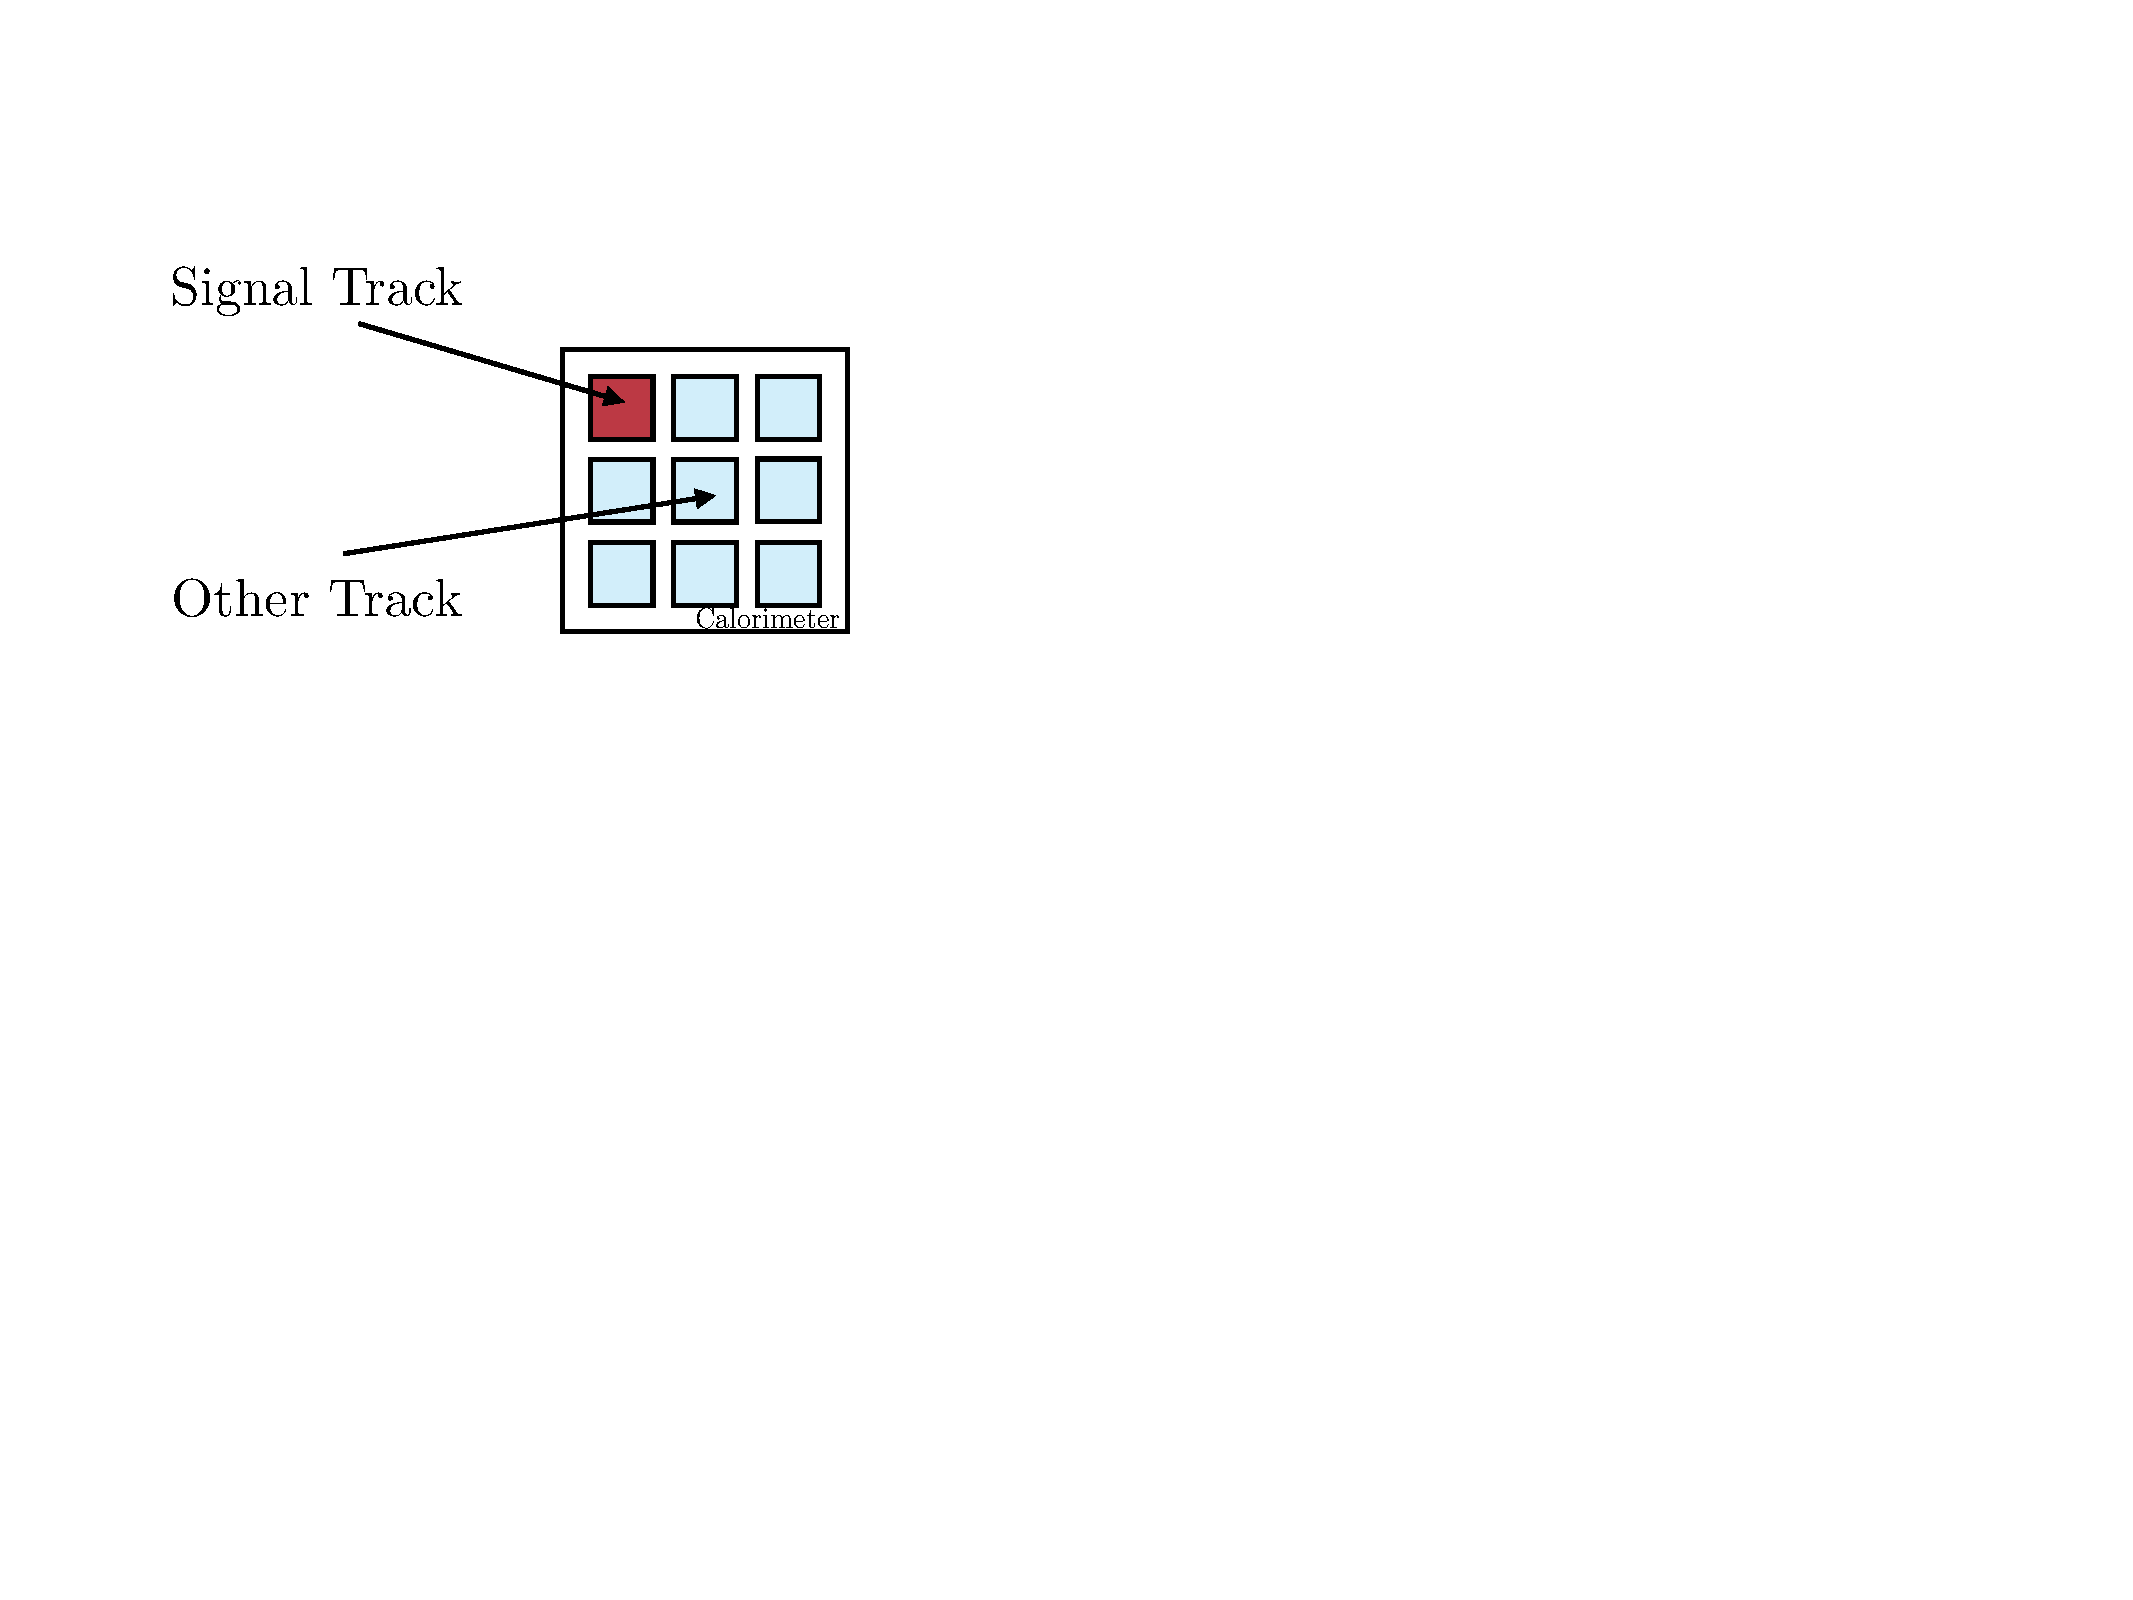
\includegraphics[width=1.0\textwidth]{figs/Selection/Tos.pdf}
        \caption{\texttt{TOS}}
        \label{fig:TOS}
    \end{subfigure}%
    \begin{subfigure}[t]{0.4\textwidth}
        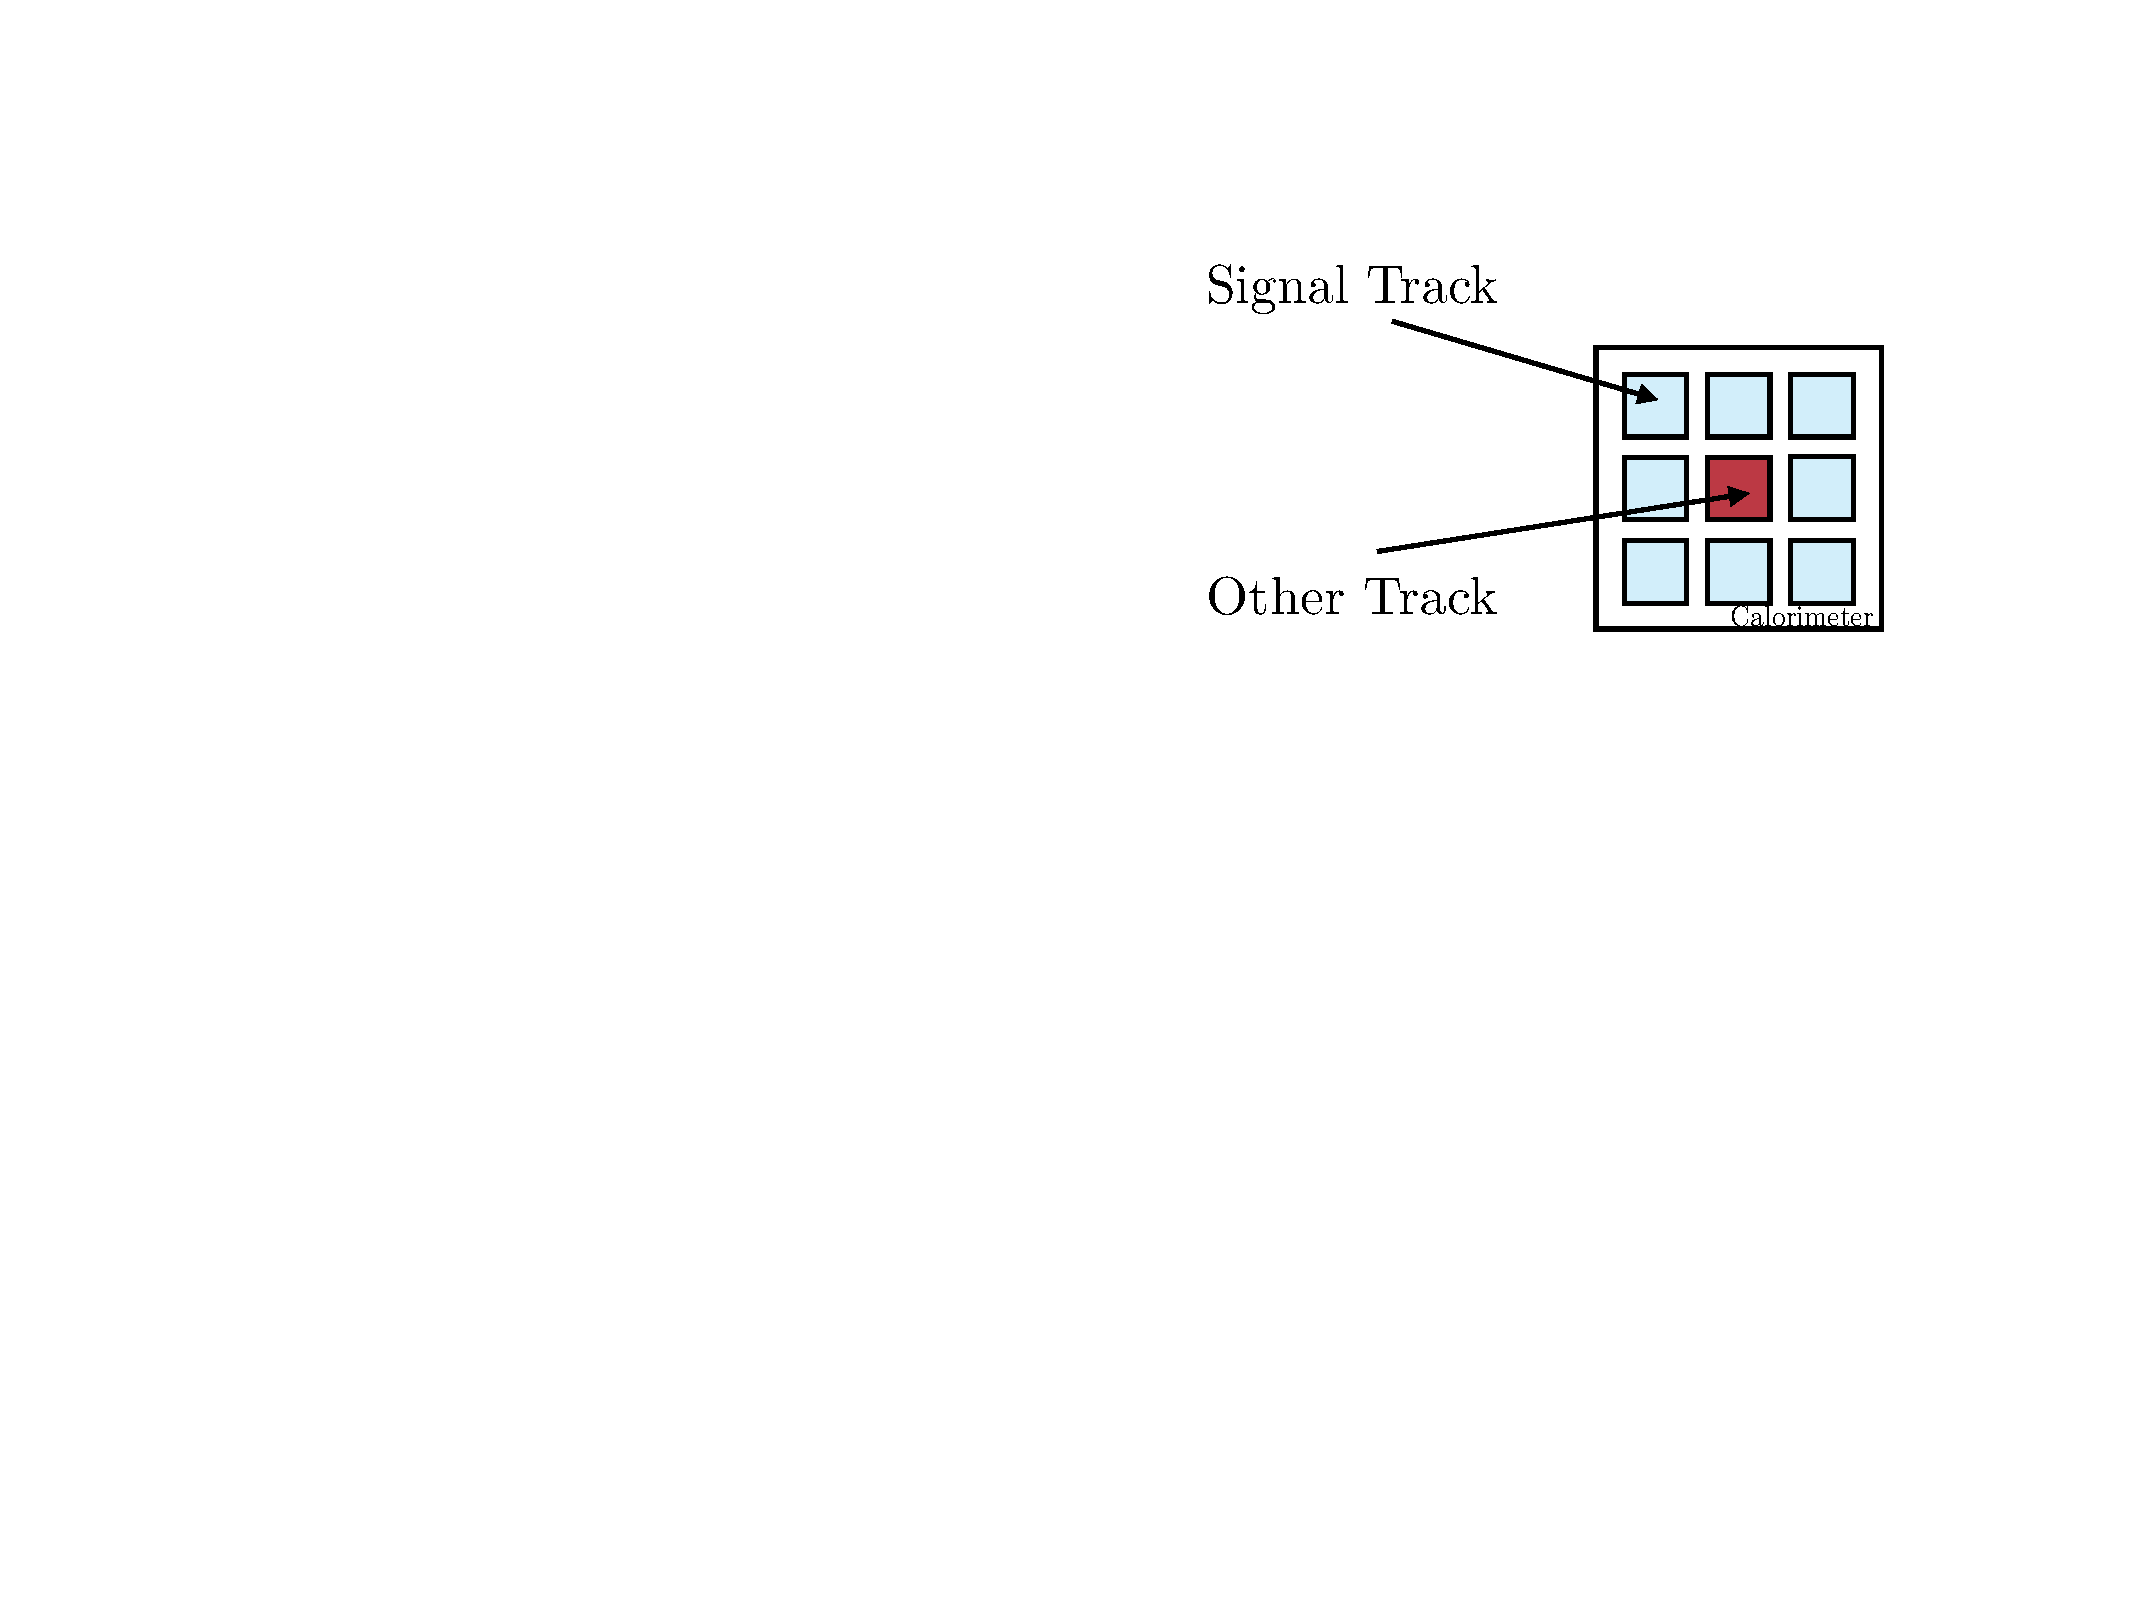
\includegraphics[width=1.0\textwidth]{figs/Selection/Tis.pdf}
        \caption{\texttt{TIS}}
        \label{fig:TIS}
    \end{subfigure}\\
    \begin{subfigure}[t]{0.4\textwidth}
        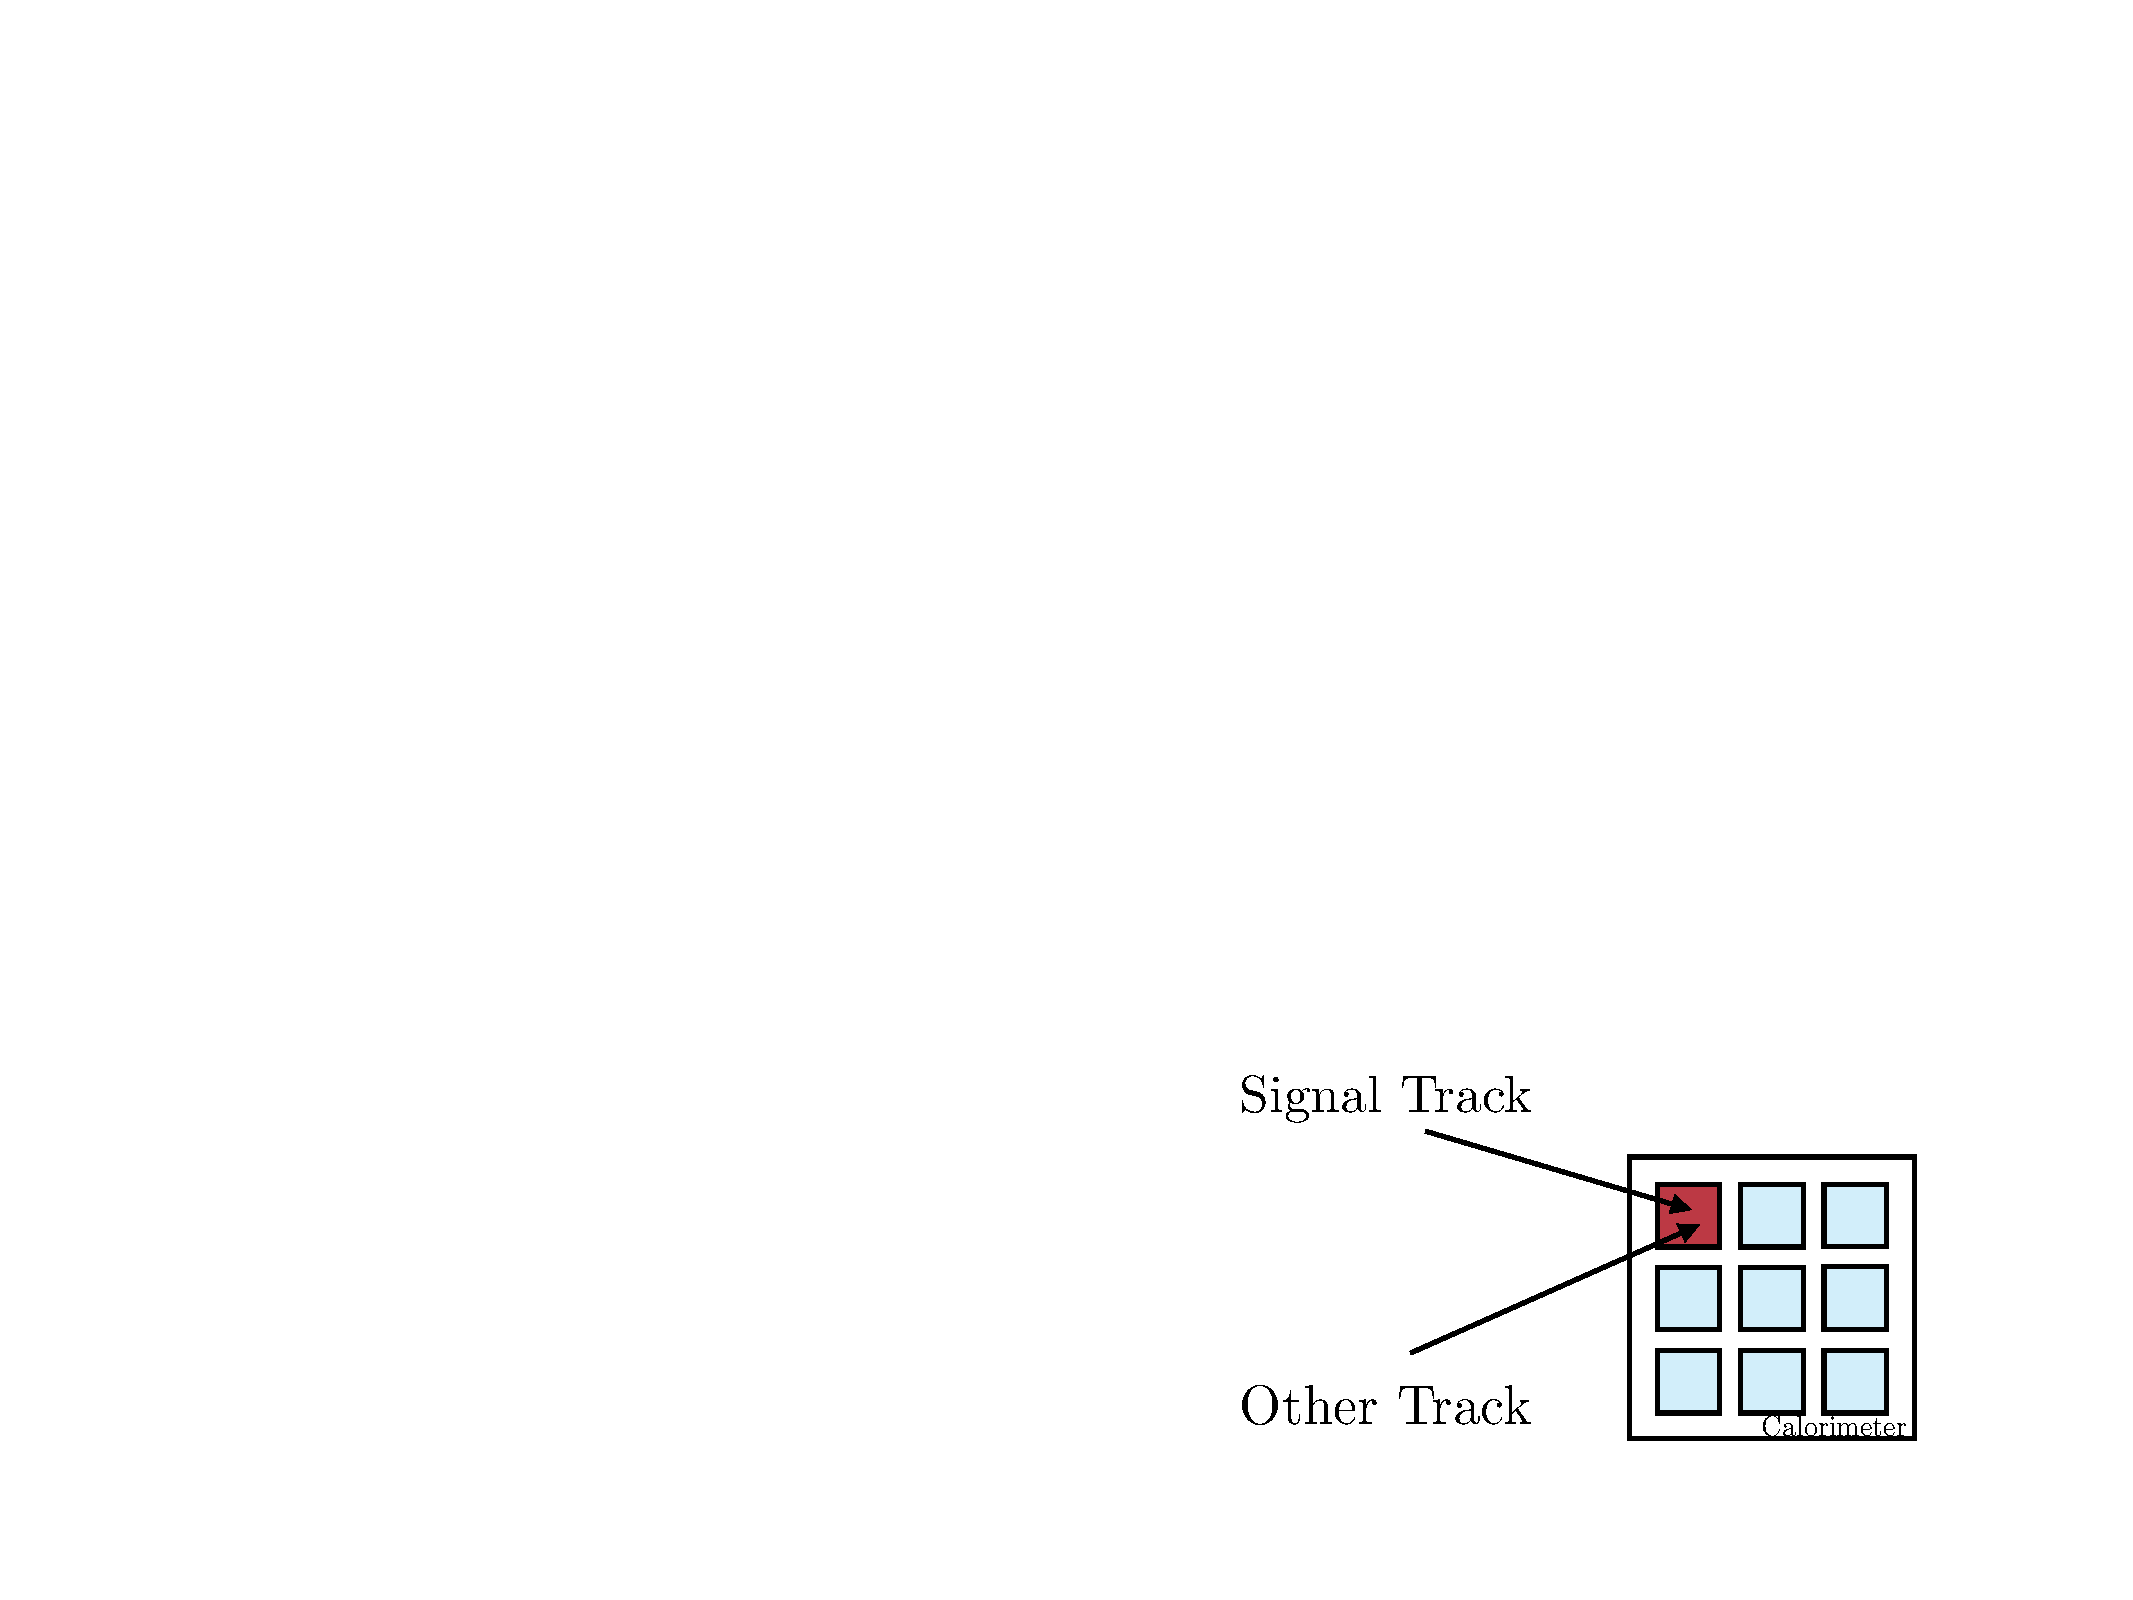
\includegraphics[width=1.0\textwidth]{figs/Selection/Tob.pdf}
        \caption{\texttt{TOB}}
        \label{fig:TOB}
    \end{subfigure}
    \begin{subfigure}[t]{0.4\textwidth}
        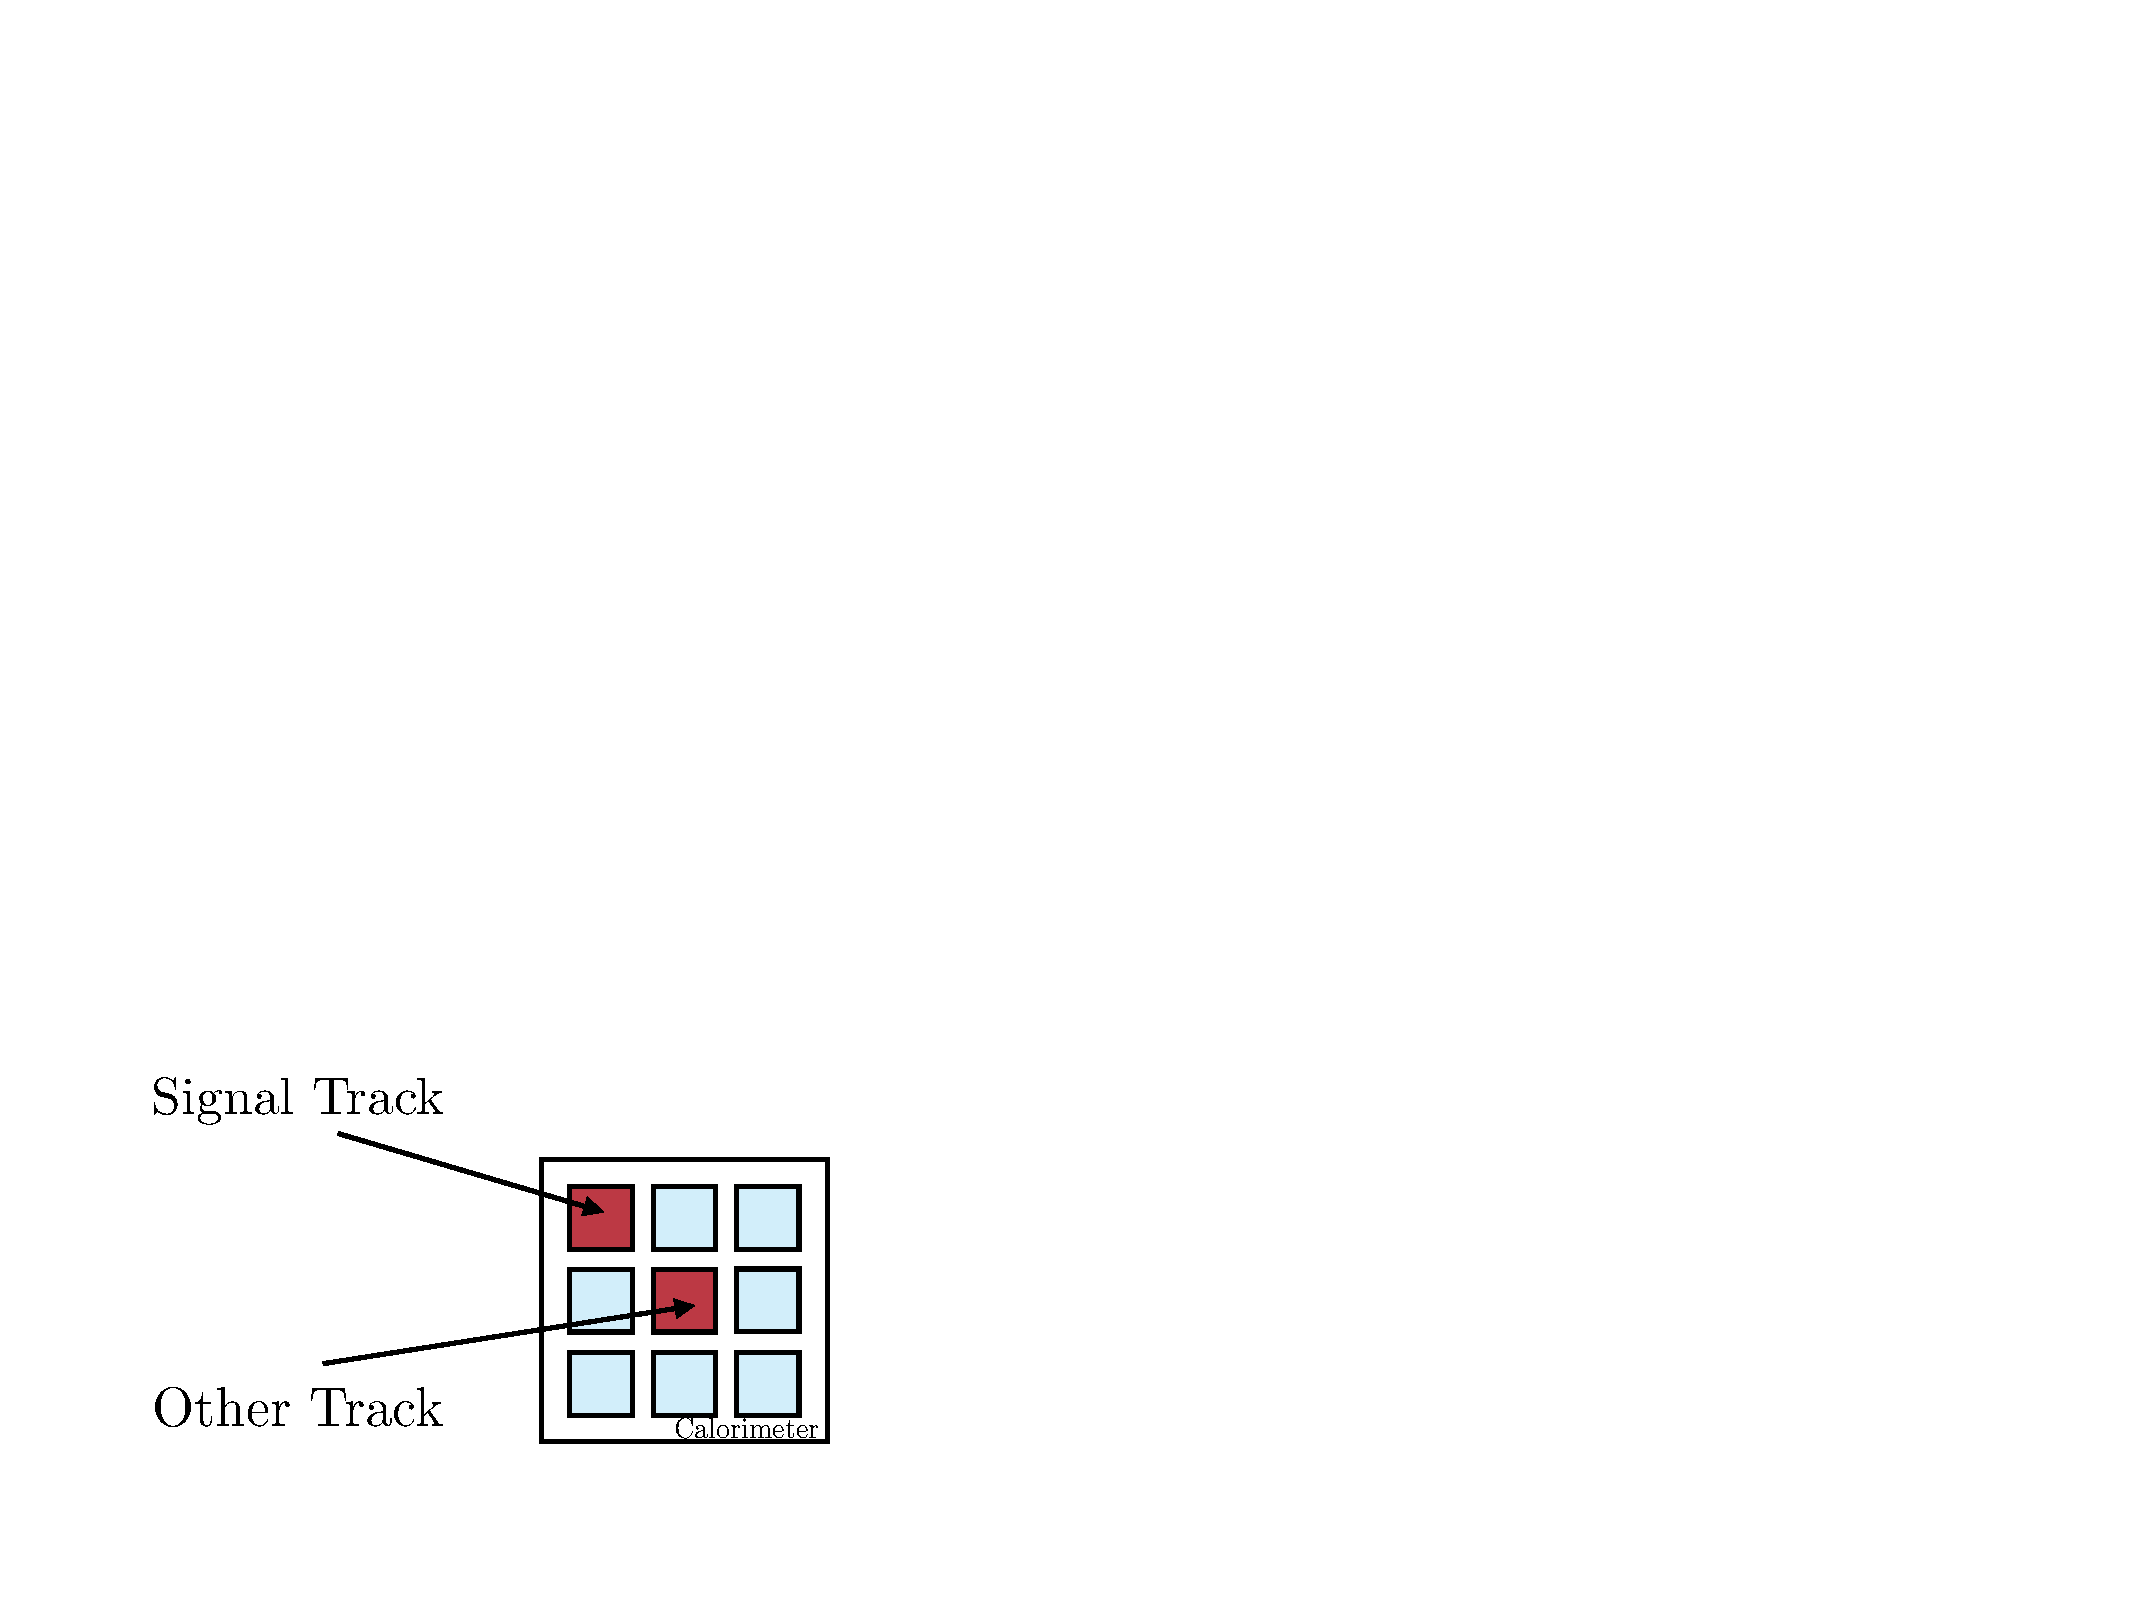
\includegraphics[width=1.0\textwidth]{figs/Selection/TisTos.pdf}
        \caption{\texttt{TOS} and \texttt{TIS}}
        \label{fig:TOSandTIS}
    \end{subfigure}\\
    \caption{Simple schematics of the different trigger matching possibilities, illustrated with one signal track and one non-signal track. Cells with a deposit above the trigger threshold are shown in red. }
    \label{fig:tistostobbing}   
\end{figure}
%%%%%%%%%%%%%%%%%%%%%%%%%%%%%%%%%%%%%%%%%%%%%%%%%%%%%%%%%%


At the hardware trigger stage, the selected candidates are required to be \texttt{TOS} with respect to the hadronic hardware trigger (\texttt{L0Hadron}). This ensures the selected candidates were retained due to corresponding deposits in the hadronic calorimeter. 
Alternatively, the logical `or' of each of the hardware sub-systems (Muon, DiMuon, Electron, Photon or Hadron) is combined into a global hardware trigger called \texttt{L0Global}.
Candidates are selected if they are \texttt{TIS} with respect to this combination.
%Alternatively, candidates are selected if they are \texttt{TIS} with respect to the global hardware trigger \texttt{L0Global}; any of the hardware trigger subsystems can contribute to the \texttt{L0Global} decision. 
This allows a second source of decays; those events where the other \bquark quark in a \bquark\bquarkbar pair production has been selected by the trigger. 


%This allows candidates that have been retained due another highly energetic decay in the same event to contribute. This could be the decay of hadron resulting from the other \bquark quark in a \bquark\bquarkbar pair production. 

The relative fractions of simulated decays selected by these \texttt{L0Hadron TOS} and \texttt{L0Global TIS} requirements for \decay{\Bp}{\Dsp\phiz} decays decaying to various \Dsp final states are shown in Table~\ref{tab:tis_tos_fractions}. The fractions are normalised to the total number of signal decays passing the \texttt{L0Hadron TOS} or \texttt{L0Global TIS} trigger requirements. 

% \begin{table}[h]
%    \centering
%       \begin{tabular}{lcccc}
%          \hline
%          \Dsp decay mode                &  \texttt{TOS} \& !\texttt{TIS} & \texttt{TIS}\&!\texttt{TOS} &  \texttt{TIS}\&\texttt{TOS}&  \texttt{TIS} or \texttt{TOS}\\
%          \hline 
%          \decay{\Dsp}{\Kp\Km\pip}       & $34.0\%$                   &$40.0\%$                   &$22.9\%$                   &$96.9\%$\\
%          \decay{\Dsp}{\Kp\pim\pip}      & $34.9\%$                   &$38.3\%$                   &$23.8\%$                   &$96.9\%$\\
%          \decay{\Dsp}{\pip\pim\pip}     & $35.9\%$                   &$37.5\%$                   &$23.5\%$                   &$96.9\%$\\
%          \hline
%       \end{tabular}
%    
%    \caption{The fraction of simulated \decay{\Bp}{\Dsp\phiz} decays in each of the hardware trigger categories for the Run I conditions. Here \texttt{TOS} refers to candidates found to be \texttt{TOS} with respect to the \texttt{L0Hadron} trigger, and \texttt{TIS} to candidates found to be \texttt{TIS} with respect to the \texttt{L0Global} requirement. The percentages are given relative to the number of decays passing the reconstruction requirements.}
%    \label{tab:tis_tos_fractions}
% \end{table}
\begin{table}[h]
   \centering
      \begin{tabular}{lccc}
         \hline
         \Dsp decay mode                &  \texttt{TOS} \& !\texttt{TIS} & \texttt{TIS}\&!\texttt{TOS} &  \texttt{TIS}\&\texttt{TOS}\\
         \hline 
         \decay{\Dsp}{\Kp\Km\pip}       & $35.1\%$                   &$41.2\%$                   &$23.7\%$       \\
         \decay{\Dsp}{\Kp\pim\pip}      & $38.0\%$                   &$36.7\%$                   &$25.3\%$       \\
         \decay{\Dsp}{\pip\pim\pip}     & $41.3\%$                   &$31.9\%$                   &$26.8\%$       \\
         \hline
      \end{tabular}
   
   \caption{The fraction of simulated \decay{\Bp}{\Dsp\phiz} decays in each of the hardware trigger categories for the Run I conditions. Here \texttt{TOS} refers to candidates found to be \texttt{TOS} with respect to the \texttt{L0Hadron} trigger, and \texttt{TIS} to candidates found to be \texttt{TIS} with respect to the \texttt{L0Global} requirement. The percentages are given relative to the total number of decay selected by the logical `or' of the two requirements.}
   \label{tab:tis_tos_fractions}
\end{table}

The software trigger stage is split into two parts, \hltone and \hlttwo.
The first stage, \hltone, performs pattern recognition on hits in the \velo and extrapolates tracks forward to the other tracking stations. At least one well reconstructed track is required. This means the track must be significantly displaced from the primary interaction and with $\pt > 1.7 \gevc$. In Run II, this trigger was reimplementing using a multivariate analysis. 

%????????????????????????
% An second algorithm is included to select pairs of high transverse momentum tracks that form a vertex that is displaced from the primary interaction. The signal candidate is required to be \texttt{TOS} with respect to these trigger lines such that two of the $\Dsp h^{+}h^{-}$ candidate tracks passes this requirement.   
%????????????????????????

At the second software stage, \hlttwo, two different algorithms are used to select $\Dsp h^{+}h^{-}$ candidates for this analysis.
The first one uses a multivariate algorithm~\cite{BBDT} to identify the presence of a secondary vertex that has two, three or four tracks and is displaced from any PV. 
%At least one of these charged particles must have a transverse momentum $\pt > 1.7\gevc$ and be inconsistent with originating from a PV. %\chisqip with respect to any primary interaction greater than 16, where \chisqip is defined as the difference in \chisq of a given PV reconstructed with and without the considered track.
This trigger algorithm is referred to as the topological trigger.
The second algorithm selects $\phiz$ candidates decaying to two charged kaons. Each kaon must have a transverse momentum $\pt > 0.8\gevc$ and be inconsistent with originating from a PV. The invariant mass of the kaon pair must be within $20\mevcc$ of the known \phiz mass~\cite{PDG2016}.
This inclusive \phiz line is used to maximise the selection efficiencies as \phiz mesons can contribute directly to \decay{\Bp}{\Dsp\phiz} decays, as well as via the large fractions of \decay{\Dsp}{\phiz\pip} decays that contribute to the \decay{\Dsp}{\Kp\Km\pip} final state.
The relative fractions of simulated \decay{\Bp}{\Dsp\phiz} decays selected by these different trigger algorithms are listed in Table~\ref{tab:topo_incphi_fractions}. The \decay{\Dsp}{\Kp\Km\pip} simulation is generated using an amplitude model that includes the \decay{\Dsp}{\phiz\pip} contribution. As a result, it can be seen that the inclusive \phiz trigger algorithm helps to retain a larger fraction of decays. 

\begin{table}[h]
   \centering
      \begin{tabular}{lccc|c}
         \hline
         \Dsp decay mode                &  \texttt{Topo} \& !\texttt{Phi} & \texttt{Phi}\&!\texttt{Topo} &  \texttt{Topo}\&\texttt{Phi}&  \texttt{Topo} or \texttt{Phi}\\
         \hline 
         \decay{\Dsp}{\Kp\Km\pip}       & $50.9\%$                   &$4.6\%$                   &$43.1\%$                   &$98.6\%$\\
         \decay{\Dsp}{\Kp\pim\pip}      & $67.6\%$                   &$2.7\%$                   &$28.3\%$                   &$98.6\%$\\
         \decay{\Dsp}{\pip\pim\pip}     & $67.5\%$                   &$2.6\%$                   &$28.5\%$                   &$98.6\%$\\
         \hline
      \end{tabular}
   
   \caption{The fraction of simulated \decay{\Bp}{\Dsp\phiz} decays in each of the \hlttwo software trigger categories for the Run I conditions. Here \texttt{Topo} refers to candidates found to be \texttt{TOS} with respect to the topological algorithm, and \texttt{Phi} to candidates found to be \texttt{TOS} with respect to the inclusive \phiz algorithm. The fractions of selected decays are measured relative to the \hltone requirements.}
   \label{tab:topo_incphi_fractions}
\end{table}



\section{Offline selection}

Events passing any trigger requirement are saved to disk for processing offline. The stages of the offline reconstruction are detailed in this section.

\subsection{Selection requirements}
\label{sec:selectionrequirements}

The offline data samples selected by the online trigger system are reconstructed and then further processed in a procedure know within \lhcb as \emph{Stripping}. This centrally managed processing builds candidate topologies from tracks and neutral calorimeter objects in each event according to a set of predefined \emph{Stripping Lines}. Each line builds a specific candidate decay, applying a loose set of preselection requirements, including kinematic, geometric and invariant mass selections. 

The candidate \decay{\Bp}{\Dsp\phiz} and \decay{\Bp}{\Dsp\Kp\Km} decays are built using almost identical set of requirements due to the similar topologies of these decays. The \phiz meson has a lifetime of $(1.55\pm0.01)\times10^{-22}\sec$~\cite{PDG2016}, therefore the kaon decay products effectively originate at the \Bp decay vertex in a similar way to \decay{\Bp}{\Dsp\Kp\Km} decays.  The normalisation channel, \decay{\Bp}{\Dsp\Dzb}, is built similarly, however the difference in lifetime between the \Dzb and \phiz mesons necessitates slightly different selection requirements. The \Dzb meson has a lifetime of $(4.101\pm0.015)\times10^{-13}\sec$, allowing the meson to travel away from the \Bp decay vertex. Sketches of the signal and normalisation decay topologies are shown in Fig.~\ref{fig:topo}.

%%%%%%%%%%%%%%%%%%%%%%%%%%%%%%%%%%%%%%%%%%%%%%%%%%%%%%%%%%
\begin{figure}[!h]
    \centering
    \begin{subfigure}[t]{0.4\textwidth}
        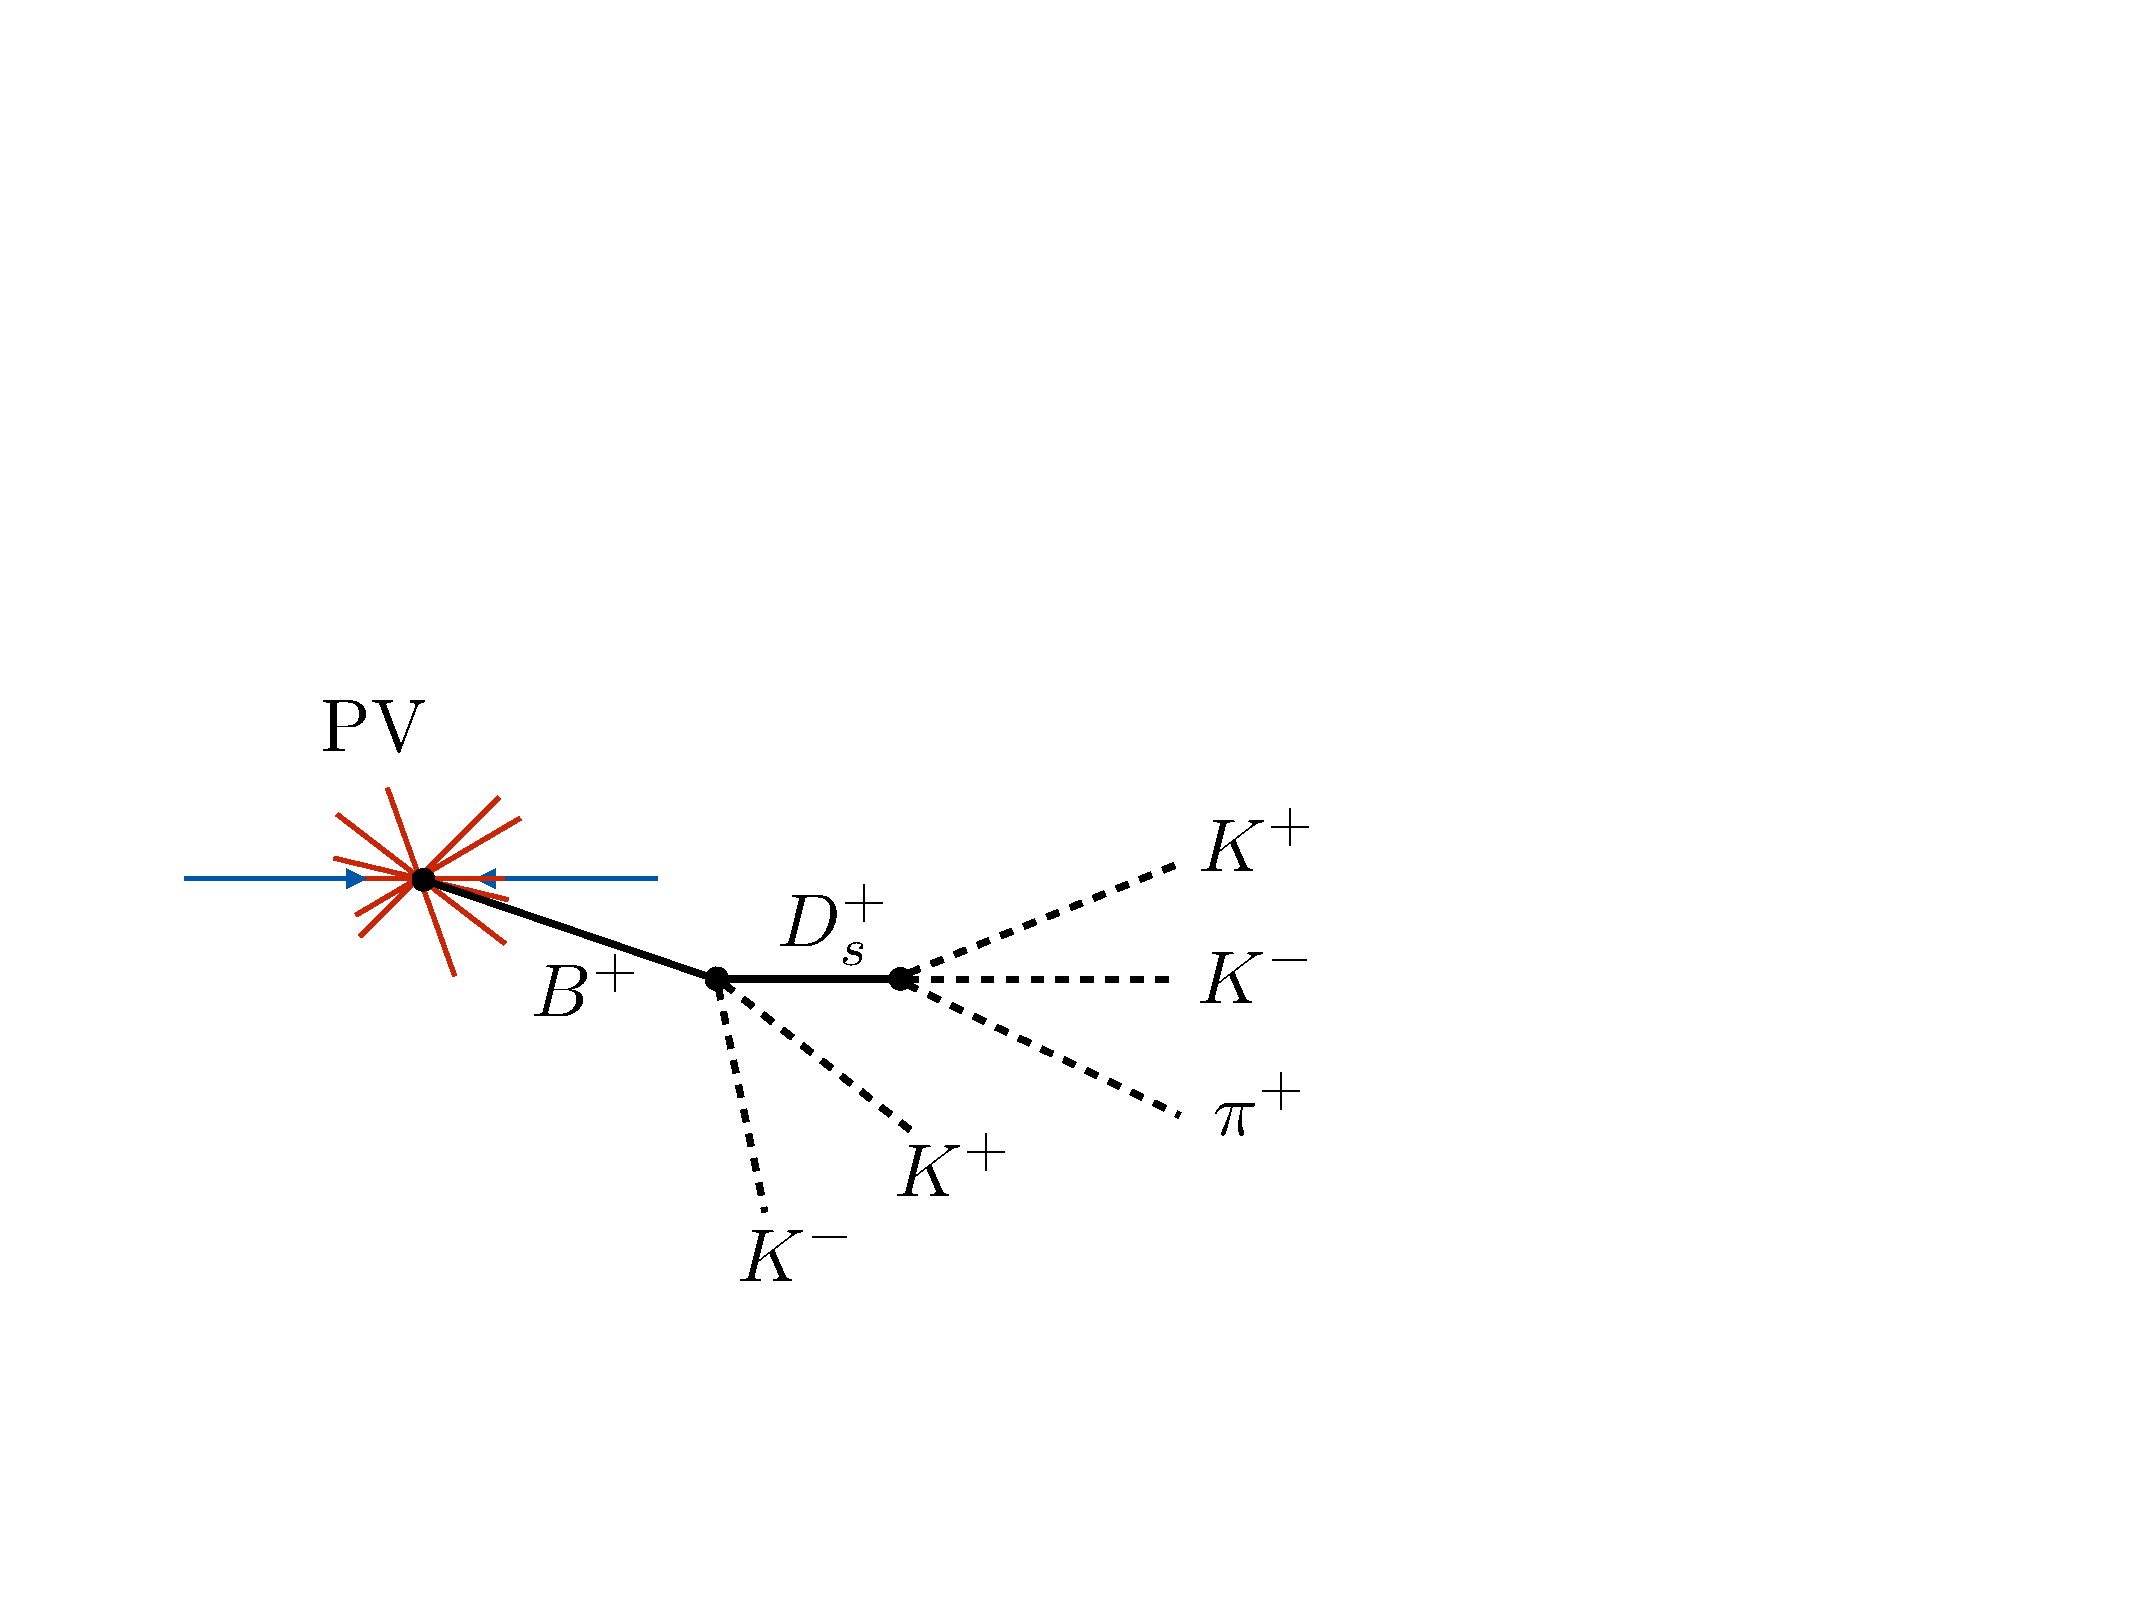
\includegraphics[width=1.0\textwidth]{figs/Selection/B2DsKK_topology.pdf}
        \caption{Signal decays}
    \end{subfigure}%
    \begin{subfigure}[t]{0.4\textwidth}
        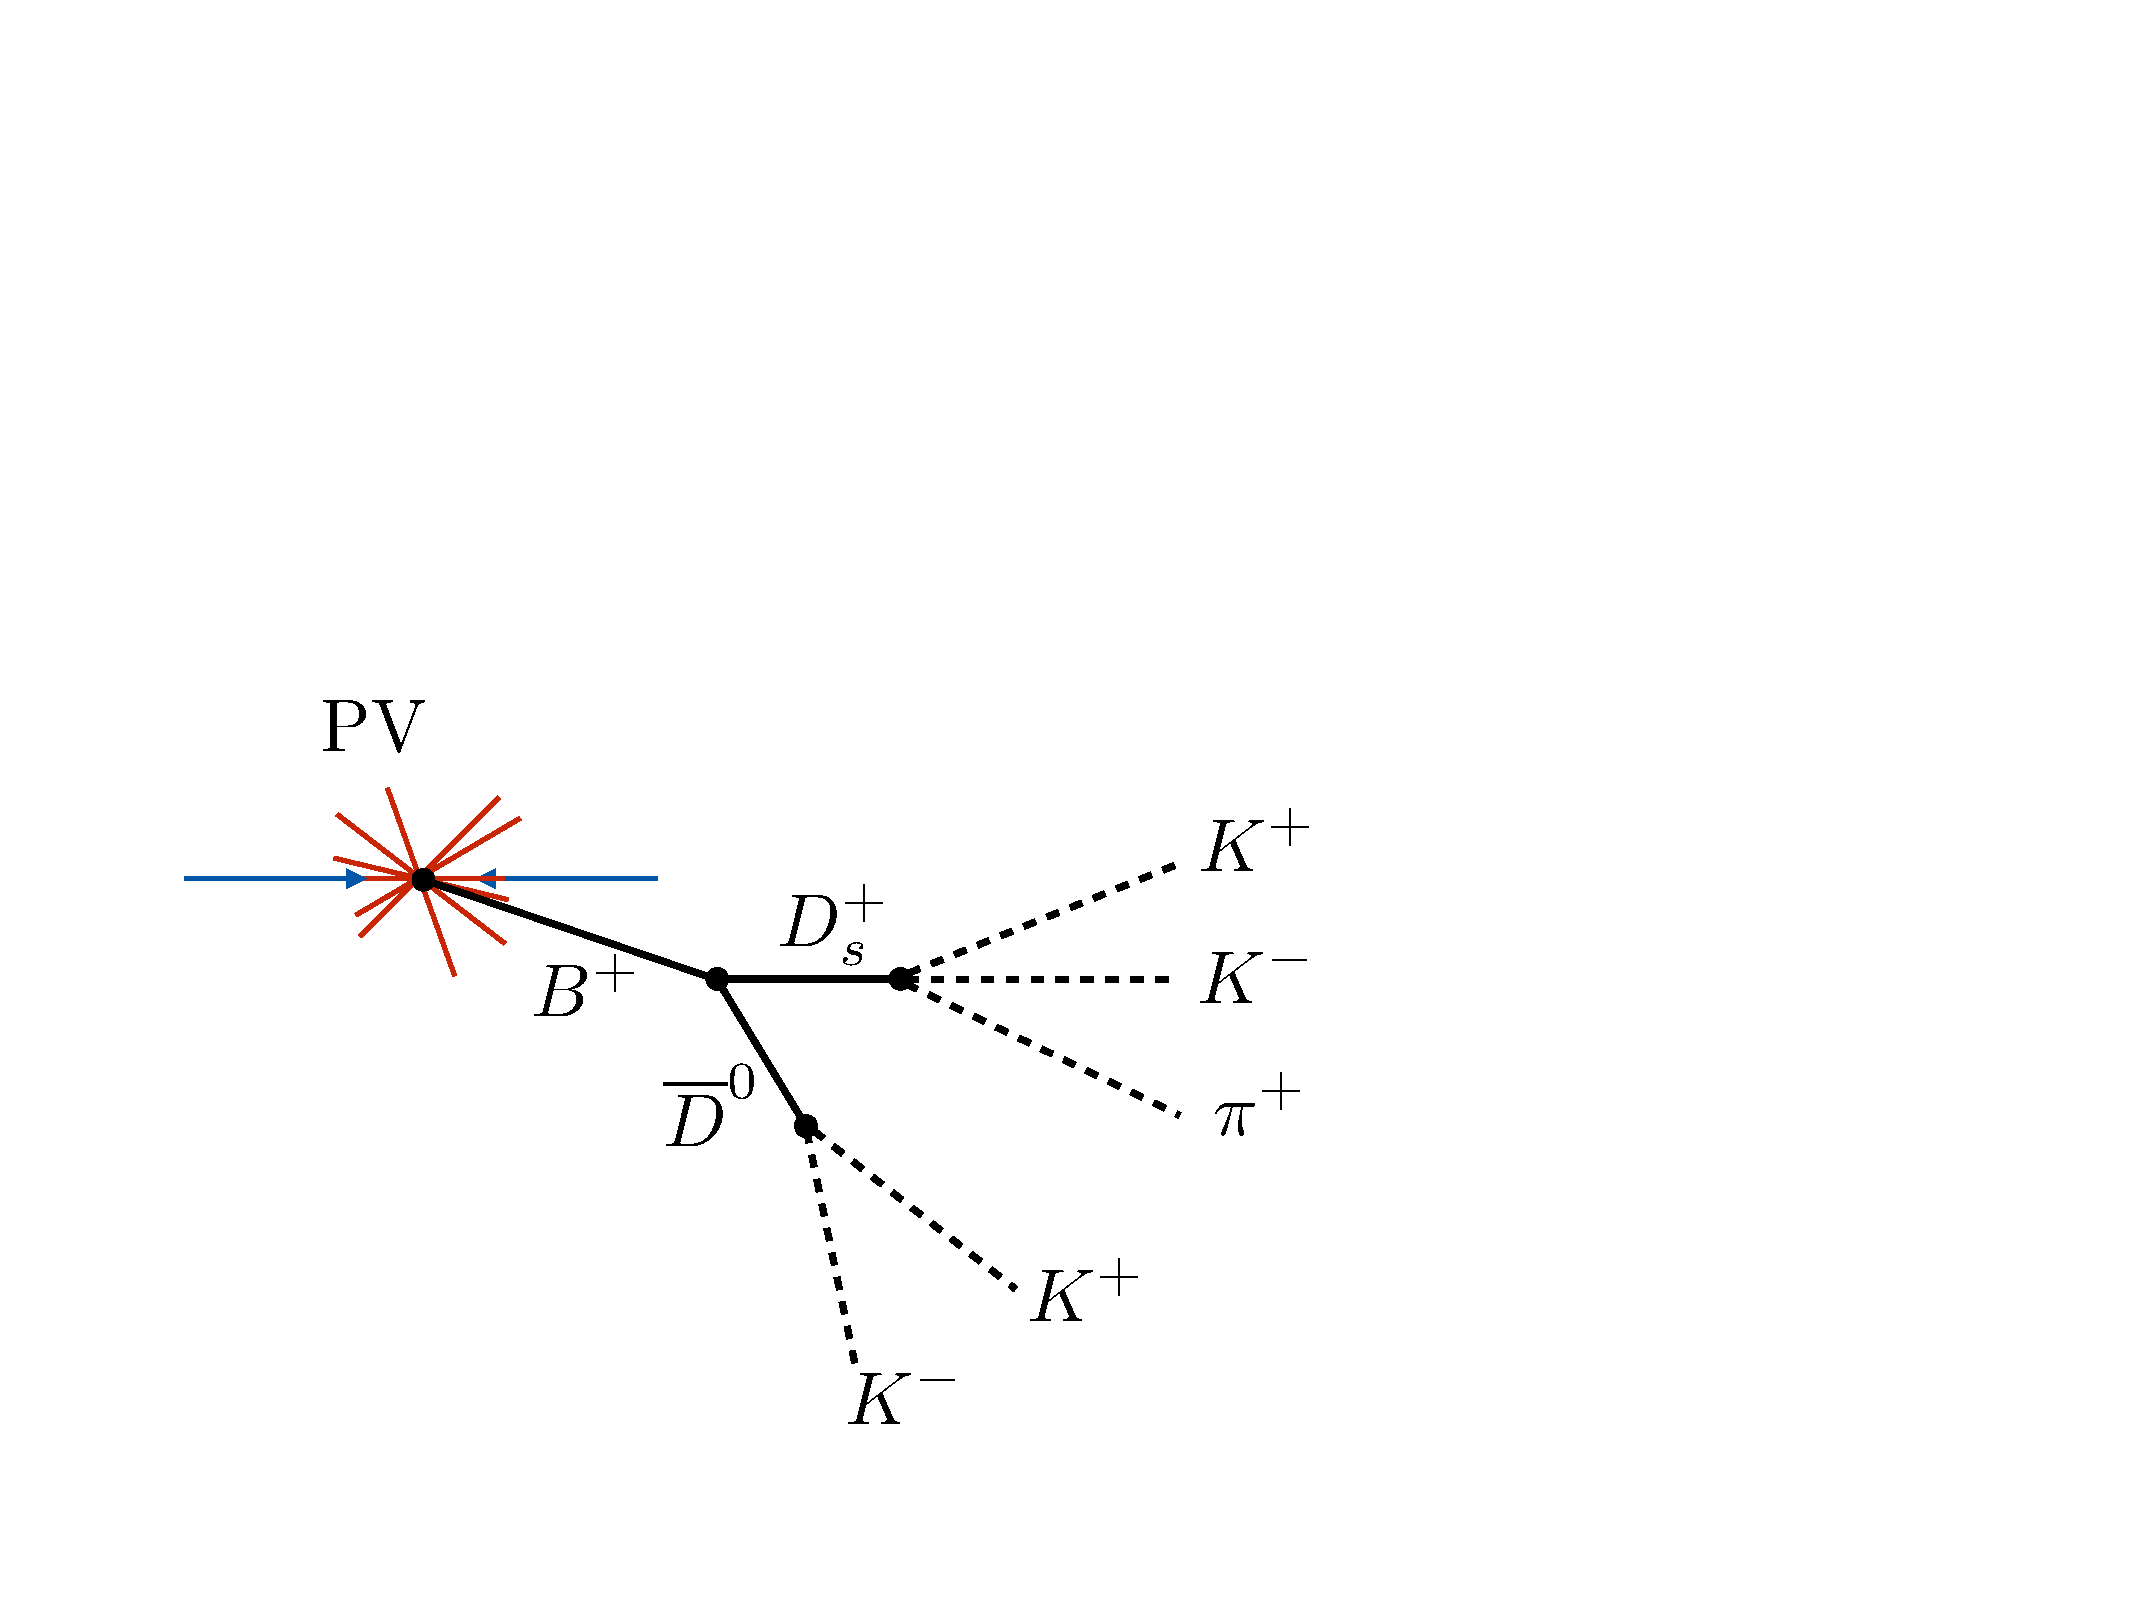
\includegraphics[width=1.0\textwidth]{figs/Selection/B2DsD0_topology.pdf}
        \caption{Normalisation decays}
    \end{subfigure}\\
    \caption{The signal and normalisation decay topologies. The collision of the two protons (blue) results in the primary collision vertex (PV). Many promptly produced tracks (red) originate at the PV. In both cases, the long-lived \Bp-meson decay vertex is displaced from the PV. The long-lived charm mesons are also displaced from the \Bp-meson decay vertex.}
    \label{fig:topo}   
\end{figure}
%%%%%%%%%%%%%%%%%%%%%%%%%%%%%%%%%%%%%%%%%%%%%%%%%%%%%%%%%%

%The candidate \decay{\Bp}{\Dsp\Kp\Km} and \decay{\Bp}{\Dsp\phiz} signal decays and \decay{\Bp}{\Dsp\Dzb} normalisation decay are reconstructed in fully hadronic final states. 
Both the \Dzb and \phiz mesons are reconstructed using pairs of oppositely charged kaons. The branching fractions are $\BF(\decay{\Dzb}{\Kp\Km})= (3.97 \pm 0.07)\times 10^{-3}$ and $\BF(\decay{\phiz}{\Kp\Km})= (48.9 \pm 0.5)\%$ respectively~\cite{PDG2016}. Although the similar two-body hadronic decay \decay{\Dz}{\Km\pip} has a larger branching fraction than mode chosen for the normalisation channel, $\BF(\decay{\Dz}{\Km\pip})= (3.89 \pm 0.04)\%$, sharing the same final state helps to reduced systematic uncertainties in the ratio of selection efficiencies. Many differences in how pions and kaons interact with the detector can be neglected as they would affect the signal and normalisation channel in the same way.
The \Dsp mesons used in the search for \decay{\Bp}{\Dsp\Kp\Km} decays are reconstructed using the \decay{\Dsp}{\Kp\Km\pip} decay. The search for the rarer \decay{\Bp}{\Dsp\phiz} decay additionally includes the modes \decay{\Dsp}{\pip\pim\pip} and \decay{\Dsp}{\Kp\pim\pip} to increase the sensitivity of the search. The branching fractions for these decays are listed in Table~\ref{tab:dsbranchingfractions}. In each instance the normalisation channel is reconstructed using the same \Dsp decay mode as the signal.  


\begin{table}[h]
   \centering
      \begin{tabular}{lccc}
         \hline
         Decay                            &\Dsp\phiz   &\Dsp\Kp\Km   &  Branching fraction \\
         \hline 
         \decay{\Dsp}{\Kp\Km\pip}         &\checkmark   &\checkmark   & $5.45 \pm 0.17 \%$ \\
         \decay{\Dsp}{\pip\pim\pip}       &\checkmark   & -  & $1.09 \pm 0.05 \%$ \\
         \decay{\Dsp}{\Kp\pim\pip}        &\checkmark   & -   & $0.66 \pm 0.04 \%$ \\
         \hline
      \end{tabular}
   
   \caption{The branching fractions for the different \Dsp decay modes used to reconstruct the signal and normalisation modes. The \Dsp decay modes contributing to the different searches are highlighted.}
   \label{tab:dsbranchingfractions}
\end{table}

%The searches for \decay{\Bp}{\Dsp\phiz} and \decay{\Bp}{\Dsp\Kp\Km} decays employ the use of two different \emph{Stripping Lines} as detailed in Table~\ref{tab:strippinglines}. These differ only in the invariant mass window applied to the $\Kp\Km$ pair used to reconstruct the $\phi$ meson, and in the number of \Dsp decay modes included: the \decay{\Bp}{\Dsp\Kp\Km} line only reconstructs the Cabibbo Favoured (CF) \decay{\Dsp}{\Kp\Km\pip} decay. The \emph{Stripping Line} used to select the normalisation channel \decay{\Bp}{\Dsp\Dzb} is also included in Table~\ref{tab:strippinglines}. This has slightly different requirements allowing the \Dzb meson decay vertex to be be displaced from the \Bp-meson decay vertex.


The selection of candidates makes requirements on many different distinguishing characteristics. The definitions of the relevant quantities are as follows:  
\begin{description}
\item \textbf{Mass, $m(X)$:} the invariant mass of the particle, or combination of particles, $X$. 
\item \textbf{Momentum, \ptot:} the magnitude of the total momentum of the particle.
\item \textbf{Transverse momentum, \pt:} The component of the total momentum, \ptot, perpendicular to the proton beam axis (the $z$-axis).
\item \textbf{Decay Time, $\tau$:} the time taken for the candidate to travel from its production vertex to its decay vertex.
\item \textbf{Decay products' \pt scalar sum, $\sum{|\pt|}$:} the sum of the magnitudes of the transverse momentum of the decay products with respect to the proton beam axis.
\item \textbf{Vertex quality, $\chi^{2}_{\text{VTX}}$:} the minimised value of $\chi^{2}$ per degree of freedom, $\chi^{2}/N_{\text{DOF}}$, as determined in the fit to the vertex location.
\item \textbf{Track quality, $\chi^{2}_{\text{TRK}}$:} the minimised value of $\chi^{2}/N_{\text{DOF}}$ as determined in the fit to the track hits.
\item \textbf{Impact parameter, $\text{IP}$:} The shortest distance between a given extrapolated track direction and a vertex location, as shown in Fig.~\ref{fig:impact_parameter}. 

%%%%%%%%%%%%%%%%%%%%%%%%%%%%%%%%%%%%%%%%%%%%%%%%%%%%%%%%%%
\begin{figure}[!h]
    \centering
    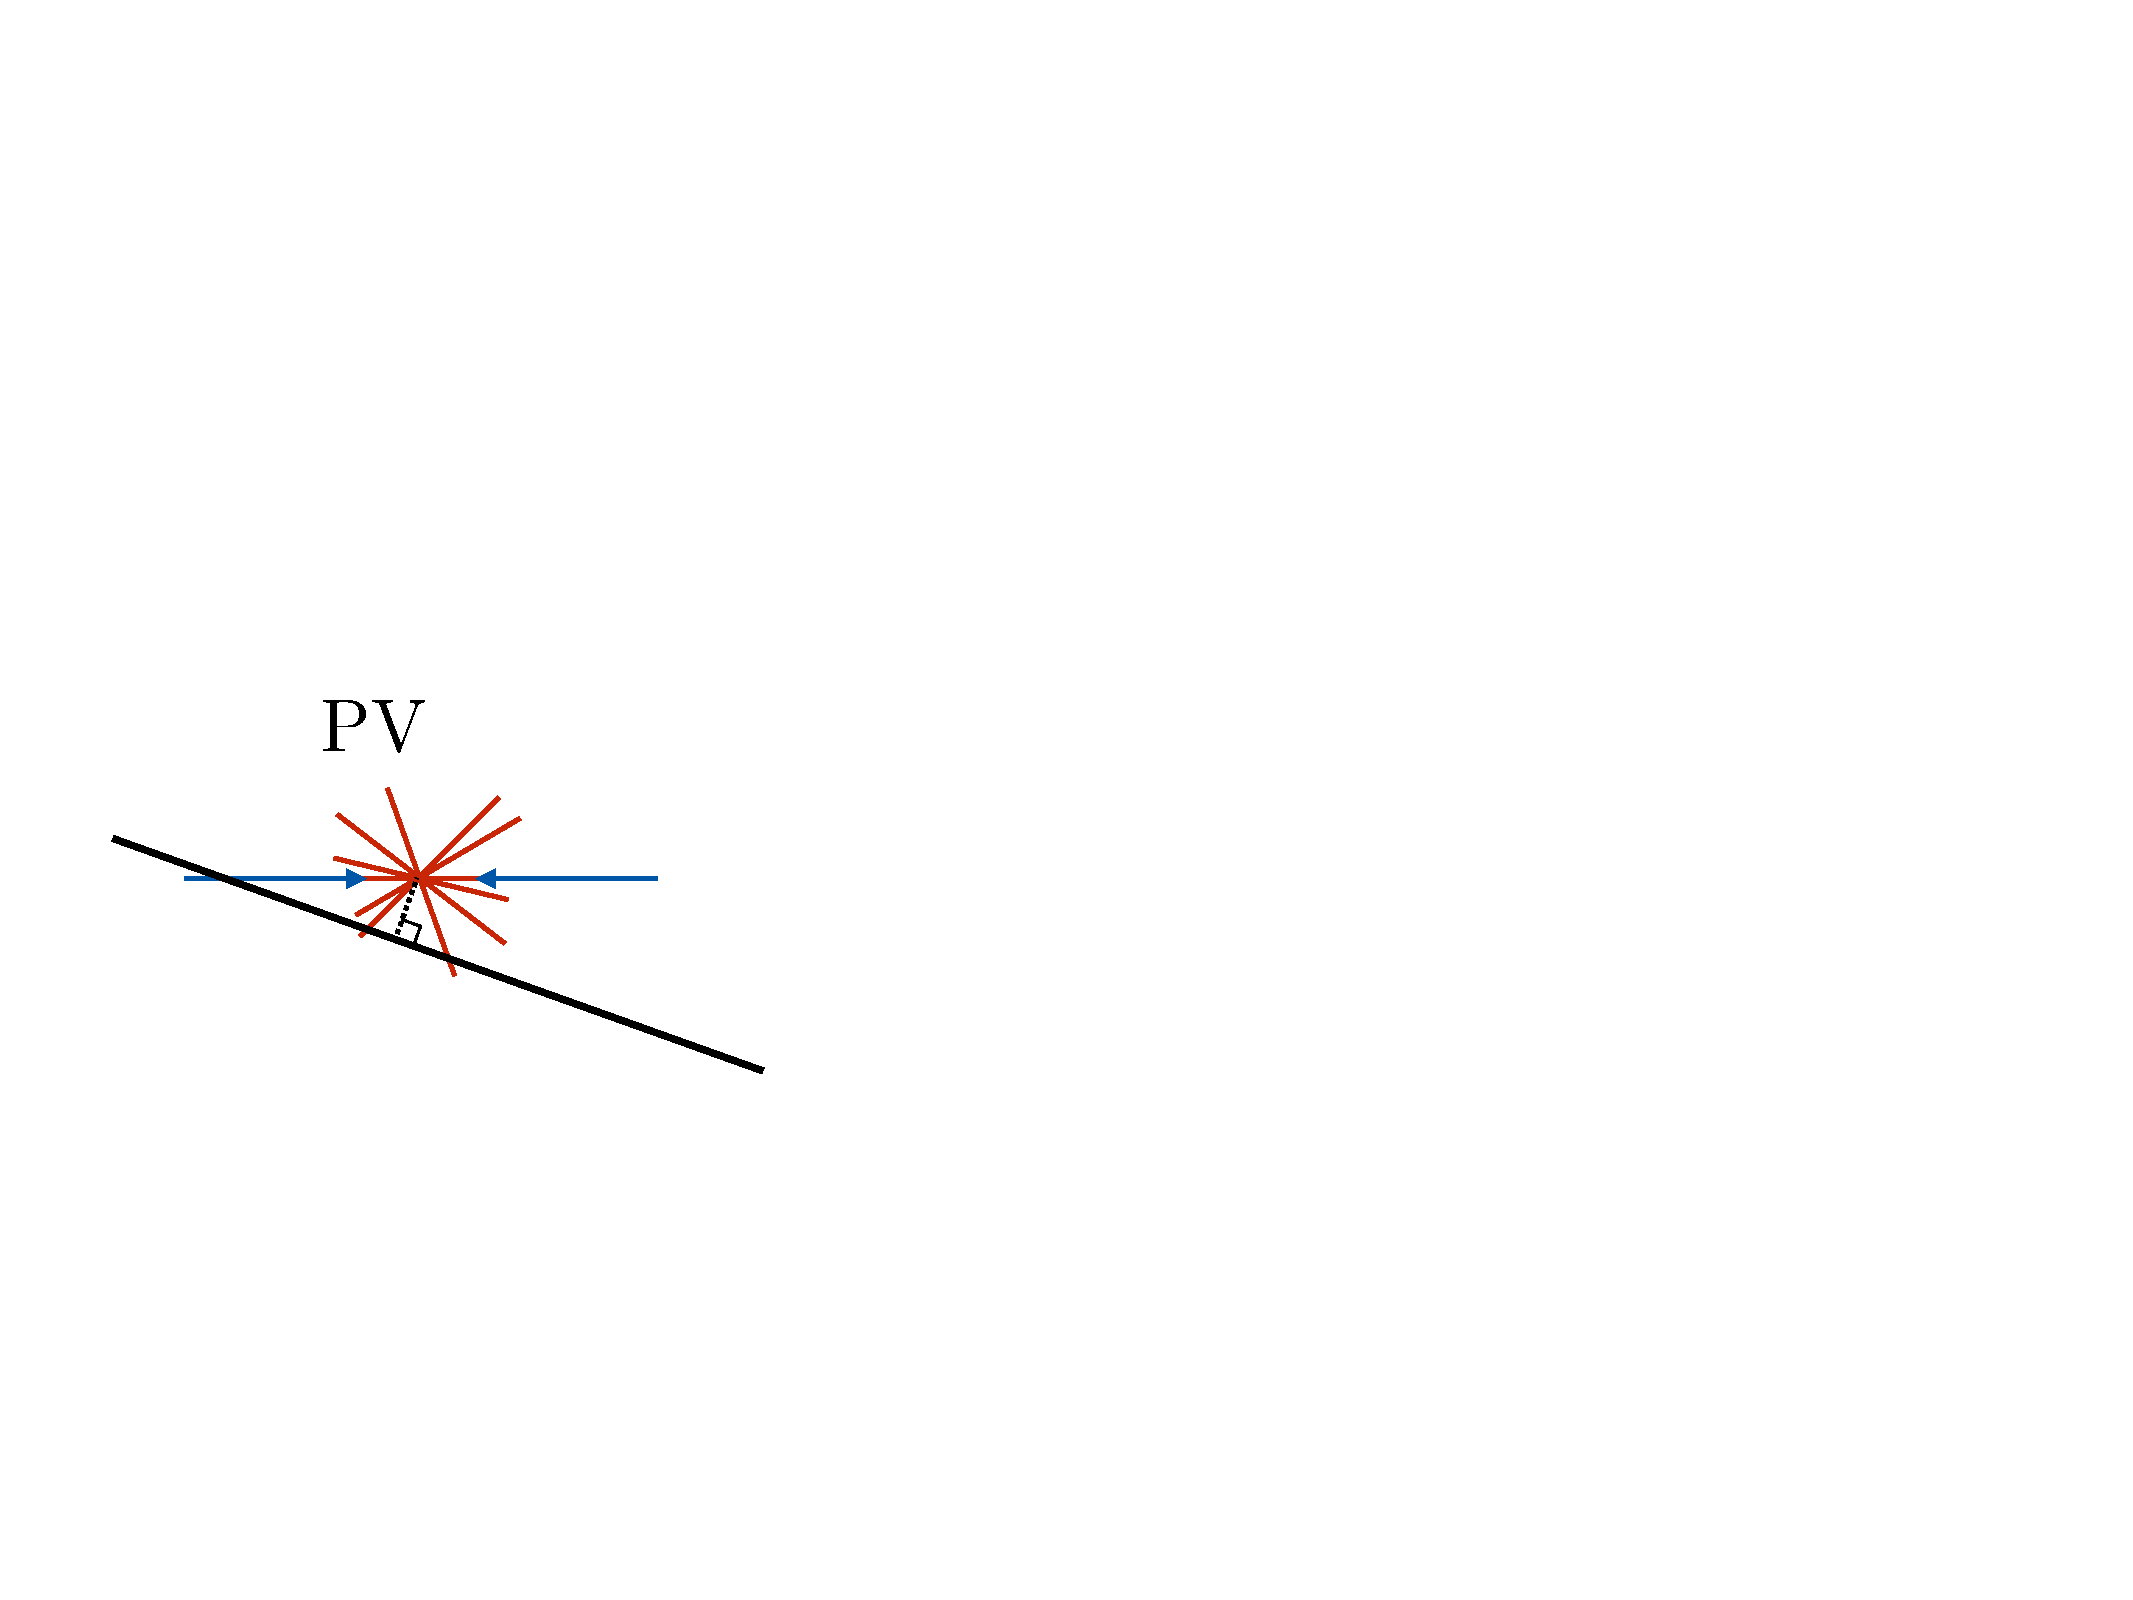
\includegraphics[width=0.4\textwidth]{figs/Selection/Impact_parameter.pdf}
    \caption{Impact parameter (dotted black line) between a track (black) and a vertex.}
    \label{fig:impact_parameter}   
\end{figure}
%%%%%%%%%%%%%%%%%%%%%%%%%%%%%%%%%%%%%%%%%%%%%%%%%%%%%%%%%%

\item \textbf{Impact parameter significance, $\chi^{2}_{\text{IP}}$:} The difference of a given vertex's $\chi^{2}/N_{\text{DOF}}$ with and without a specific track included in the fitting procedure.
\item \textbf{Flight distance significance, $\chi^{2}_{\text{FD}}$:} A measure of how significant the flight distance of a combination of particle is. This is defined as the $\chi^{2}$ associated with the difference in position of the two vertices, $\vec{\mathbf{d}} = \vec{\mathbf{v}}_2 - \vec{\mathbf{v}}_1$, where $\vec{\mathbf{v}}_1$ and $\vec{\mathbf{v}}_1$ are positions of the first and the second vertices. 
\item \textbf{Distance of closest approach, $\text{DOCA}(h,h')$:} The shortest distance between two tracks as shown in Fig~\ref{fig:doca}.
%%%%%%%%%%%%%%%%%%%%%%%%%%%%%%%%%%%%%%%%%%%%%%%%%%%%%%%%%%
\begin{figure}[!h]
    \centering
    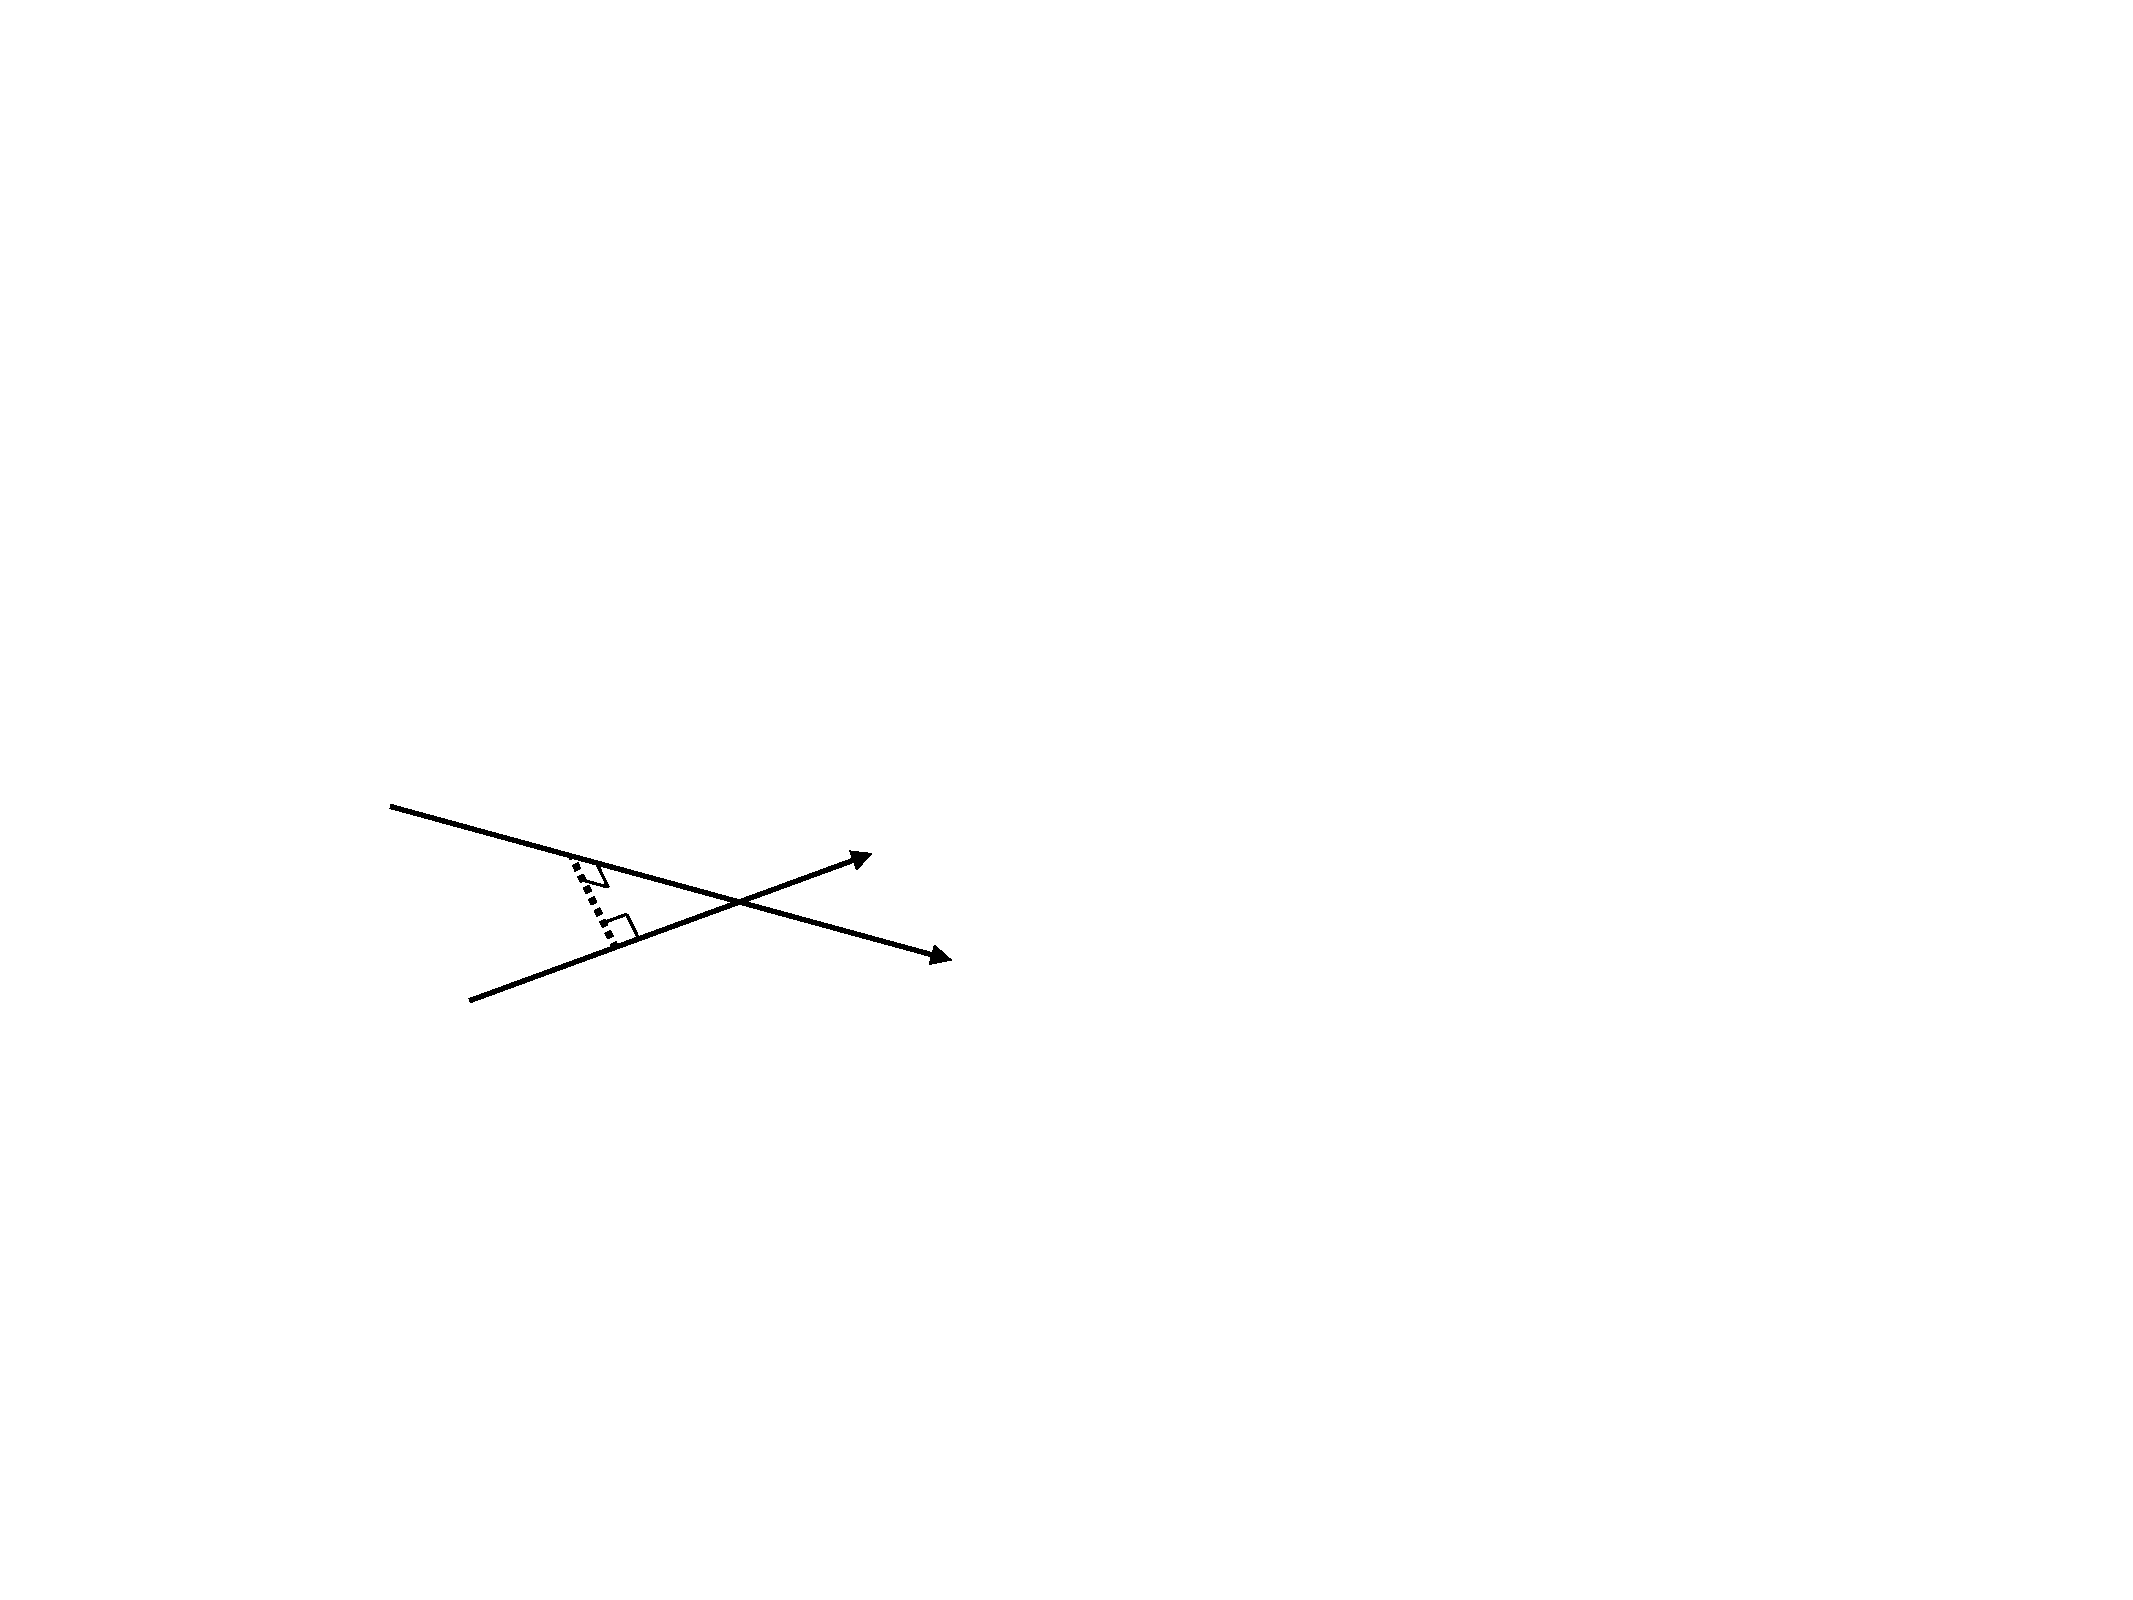
\includegraphics[width=0.4\textwidth]{figs/Selection/DOCA.pdf}
    \caption{Distance of closest approach (dotted black line) between two tracks.}
    \label{fig:doca}   
\end{figure}
%%%%%%%%%%%%%%%%%%%%%%%%%%%%%%%%%%%%%%%%%%%%%%%%%%%%%%%%%%


\item \textbf{Ghost track probability, $P_{\text{Ghost}}$:} This parameter quantifies the probability that a given track is an incorrect combination of tracking stations hits, known as a ghost track. The numerical value is the output of a Neural Network algorithm trained to separate true tracks from ghost tracks using simulated events. Various tracking parameters are inputs to the Neural Network including the number of hits in various tracking stations, the track fit quality and the number of tracks per event. 

\item \textbf{Direction angle:} The angle between a track's momentum vector and the vector connecting the primary vertex and decay vertex as shown in Fig.~\ref{fig:dira}.

%%%%%%%%%%%%%%%%%%%%%%%%%%%%%%%%%%%%%%%%%%%%%%%%%%%%%%%%%%
\begin{figure}[!h]
    \centering
    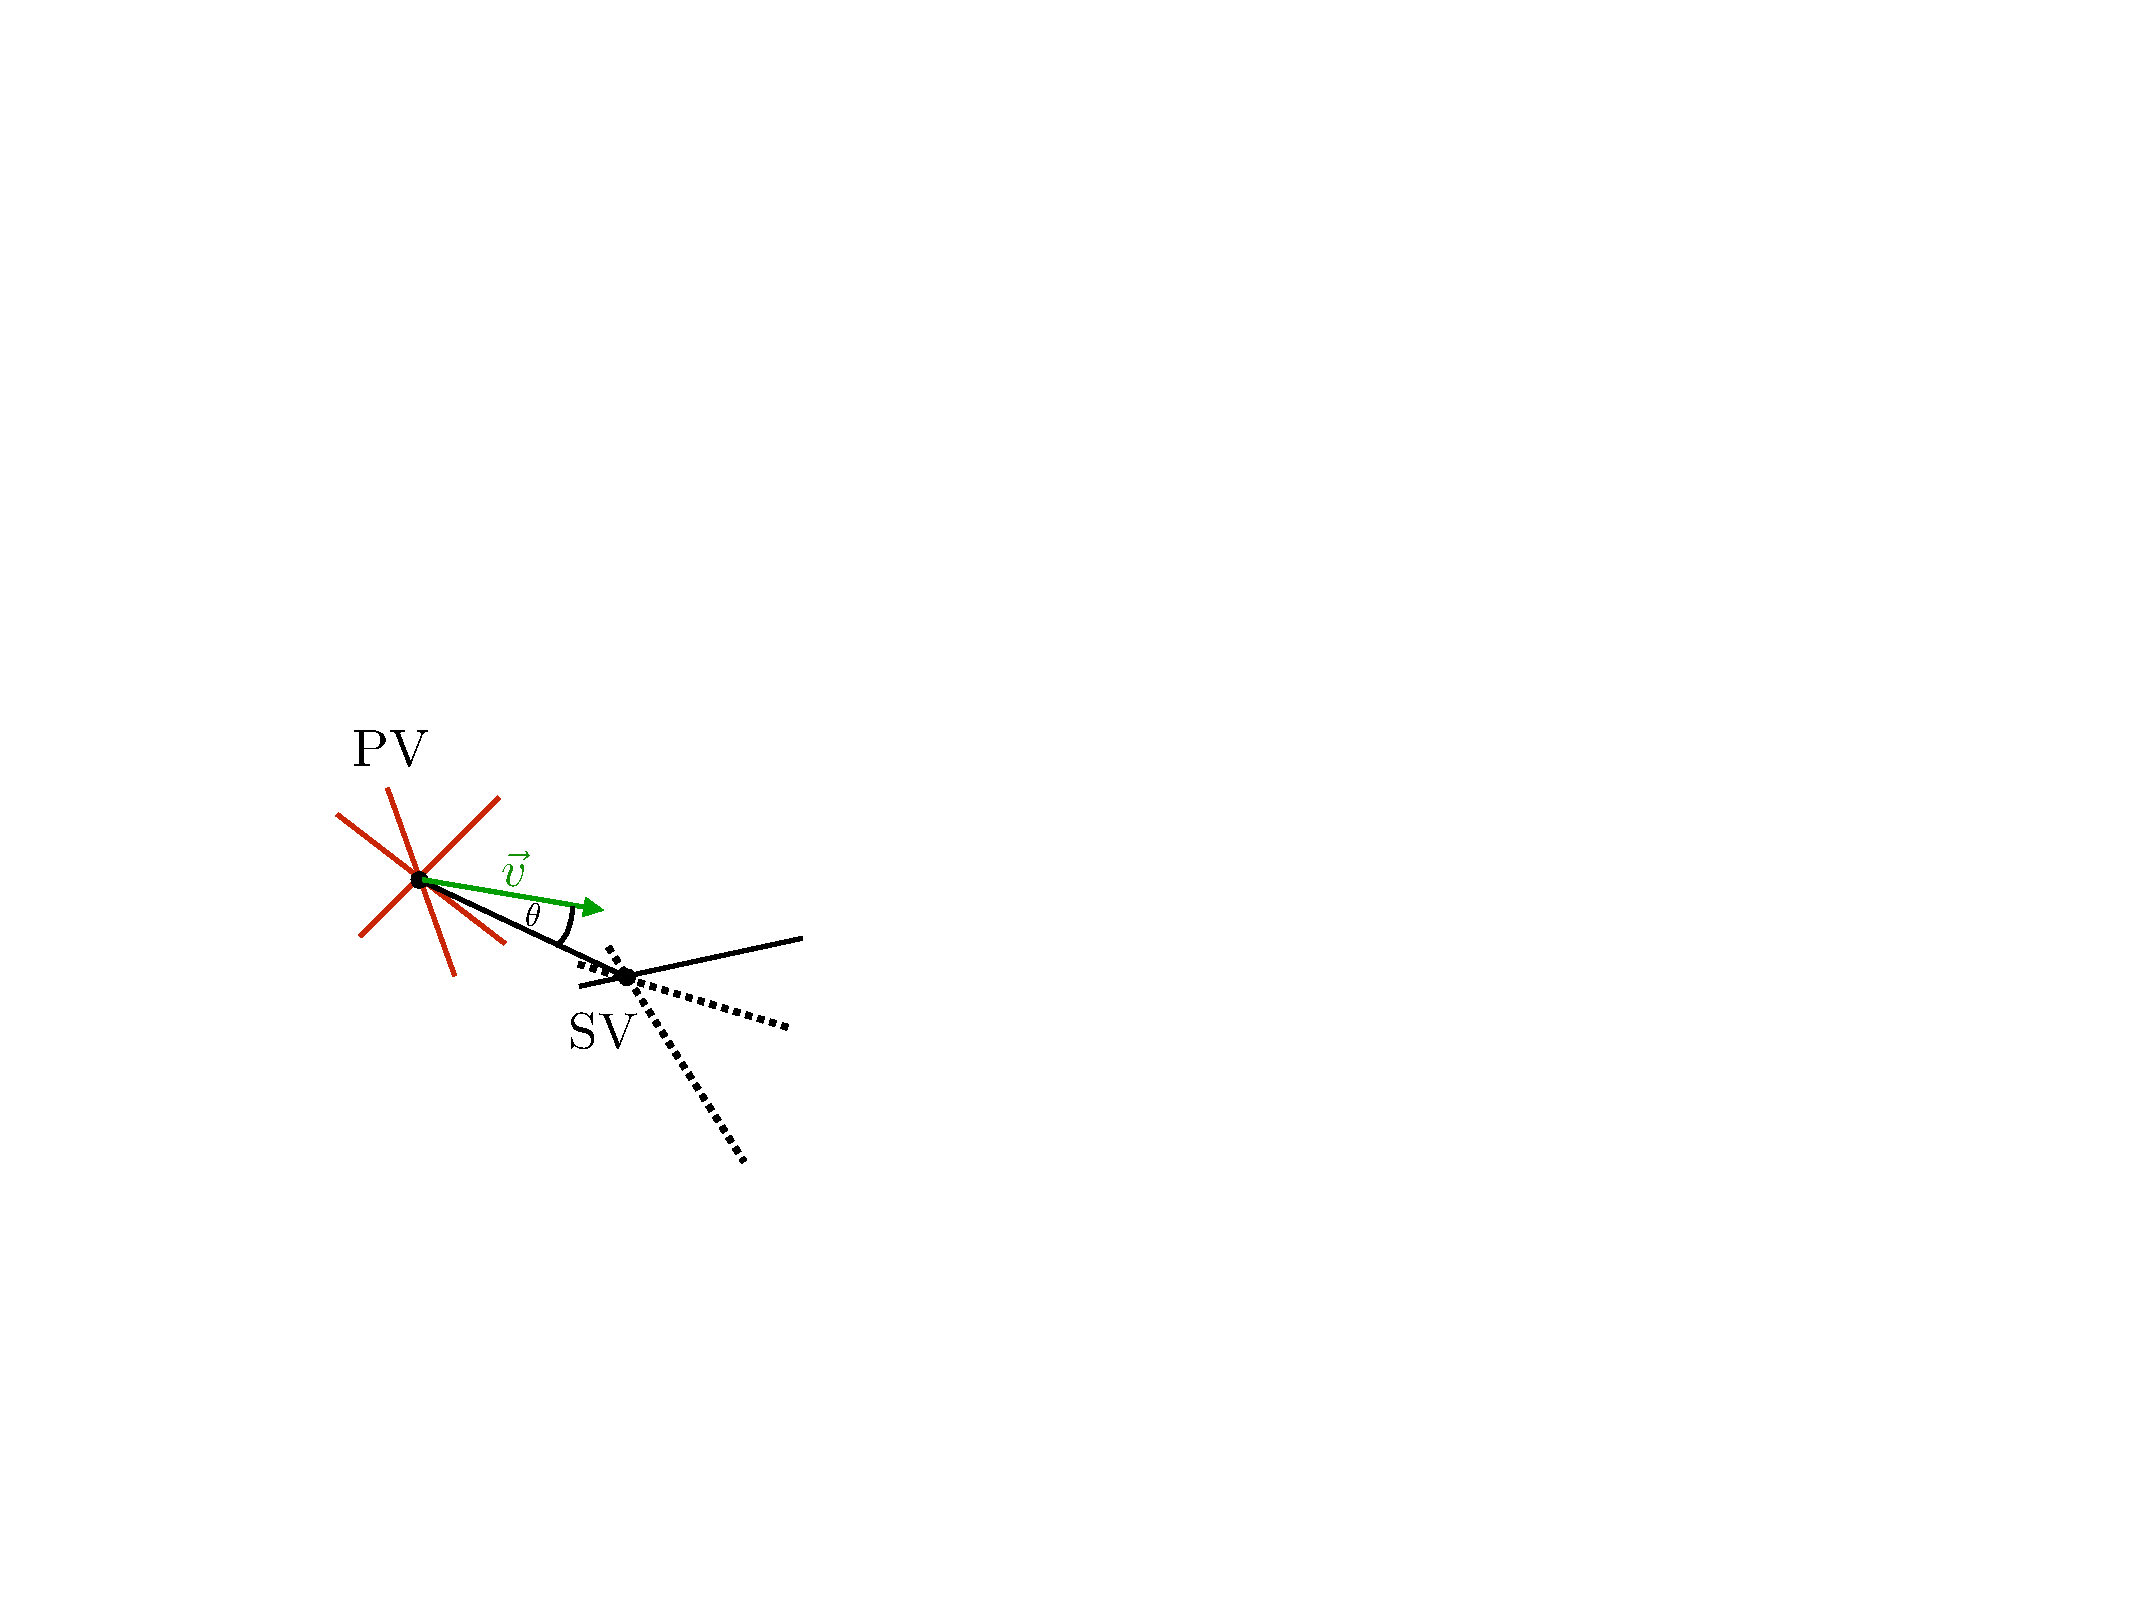
\includegraphics[width=0.4\textwidth]{figs/Selection/DIRA.pdf}
    \caption{Direction angle, $\theta$, between the line joining two vertices, primary vetex (PV) and secondary vertex (SV), and the momentum vector shown in green. The momentum vector corresponds to the momentum of the three tracks contributing to the SV. }
    \label{fig:dira}   
\end{figure}
%%%%%%%%%%%%%%%%%%%%%%%%%%%%%%%%%%%%%%%%%%%%%%%%%%%%%%%%%%


\item \textbf{Particle identification, $\text{PIDK}$:} The different in the log-likelihood of the kaon and pion hypothesis for a given track.  
\end{description}


\subsubsection{Track requirements}
As the final states are fully hadronic, the candidates are built from the combination of five \emph{long} tracks.  
% The tracks are required to meet the following criteria; 
% \begin{itemize}
% \item well reconstructed with $\chi^{2}/N_{\text{DOF}} < 4 $,
% \item $\ptot > 1000 \mevc$ and $\pt > 100 \mevc$,
% \item significant impact parameter with respect to the PV of $\chi^{2}_{\text{IP}} > 4$,
% \item loose requirements on PIDK ensure the tracks are of the required species,
% \item incorrect track candidates are suppressed with $P_{\text{Ghost}}<0.4$.
% \end{itemize} 
The track $\chi^{2}/N_{\text{DOF}}$ is required to be below $4.0$ to remove poorly reconstructed tracks, with $\ptot > 1000 \mevc$ and $\pt > 100 \mevc$.
Due to the long lifetime and high boost of the \Bp and \D mesons, the decay products originate from a vertex that is displaced from the proton-proton collision vertex. In this case the trajectory of the \Bp or \D decay products do not pass through the primary collision position. A requirement is placed on the significance of the impact parameter between the track and the PV of $\chi^{2}_{\text{IP}} > 4$ to ensure all of the tracks used are inconsistent with originating at the primary interaction.  
Loose requirements on PIDK ensure the tracks are of the required species. These are further tightened as detailed in Section~\ref{sec:pidrequirements}. Incorrect track candidates are suppressed by requiring $P_{\text{Ghost}}<0.4$. 

%%%%%% Ds/ D0 and phi construction
\subsubsection{\Dzb, \phiz and \Dsp requirements}
The tracks passing these requirements are combined in pairs or triplets to form the \Dsp and \phiz or \Dzb meson candidates.  

% The \phiz candidates (or \Kp\Km pair) are created from all combinations of two tracks meeting the following requirements:
% \begin{itemize}
% \item pass within $0.5\mm$ of one another at their closest point,
% \item well reconstructed vertex with $\chi^{2}/N_{\text{DOF}} < 16$,
% \item decay product' scalar \pt sum greater than $1000\mevc$,
% \item flight distance significance is required to be $\chi^{2}_{\text{FD} } > 16$,
% \item the direction angle is required to be $\cos{\theta}>0$, preventing the vertex being backward of the PV when the momentum is forward,
% \item for \decay{\Bp}{\Dsp\phiz} decays, $|m(\Kp\Km) -m(\phiz)| < 150\mevcc$.
% \end{itemize} 


For the purpose of forming the \phiz candidates (or \Kp\Km pair), all combinations of two tracks are considered where the tracks are assigned the kaon mass. Only pairs which pass within $0.5\mm$ of one another at their closest point are retained. 
%A number of requirements are imposed to ensure the pair are consistent with coming from a \phiz meson (or \Kp\Km pair) that originated in a \Bp-meson decay. 
The vertex is required to be of good quality, the scalar sum of the transverse momentums must be greater than $1000\mevc$ and the flight distance significance is required to be $\chi^{2}_{\text{FD} } > 16$. Additionally the cosine of the direction angle, defined to be the angle between the momentum vector and flight vector, is required to be $\cos{\theta}>0$, preventing the vertex being backward of the PV when the momentum is in the forward direction. In the search for \decay{\Bp}{\Dsp\phiz} decays, the invariant mass of the two kaons is required to be within $150\mevcc$ of the known \phiz-meson mass.  

The \Dzb meson candidates are selecting using a similar parameters, however the exact values of the cuts are changed to reflect the differences in properties of the \phiz and \Dzb mesons. The vertex quality and flight distance significance requirements are tightened to $\chi^{2}/N_{\text{DOF}} < 10$ and $\chi^{2}_{\text{FD} }  > 36$ respectively, and the scalar \pt sum requirement is increased to $\sum{|\pt|} > 1800 \mevc$. 


The \Dsp mesons candidates are created using combinations of three tracks given the mass hypotheses kaons or pions, depending on the decay mode being constructed. All combinations of three tracks are considered and only those in which all three tracks are within 0.5\mm of one another are retained. As with the \Dzb meson selection, the vertex quality, flight distance significance and scalar \pt sum requirements are $\chi^{2}/N_{\text{DOF}} < 10$, $\chi^{2}_{\text{FD} }  > 36$ and $\sum{|\pt|} > 1800 \mevc$ respectively.




%% B meson construction
\subsubsection{\Bp requirements}
The \Bp meson candidates are constructed from all possible combinations of the \Dsp and \phiz or \Dzb meson candidates in each event.
Requirements are placed on these combination to select just those consistent with \Bp mesons.
That is
\begin{itemize}
\item the combination is required to have a lifetime $\tau_{\Bp} > 0.2\ps$, 
\item the direction angle must pass the requirement $\cos{\theta}>0.999$,
\item the impact parameter significance is required to be $\chi^{2}_{\text{IP}} < 25$ to ensure the \Bp meson originated at the primary interaction, 
\item the vertex is required to have a quality of $\chi^{2}/N_{\text{DOF}} < 10$. 
\end{itemize}
%More requirements are additionally placed on the decay products that contribute to the \Bp meson. 
The full list of selection requirements are detailed in Appendix~\ref{ch:appendix_selection}. 


% \begin{table}[!h]
% \centering
% \begin{tabular}{ l l l}
% \hline
% Particle       & Quantity                       & Requirement                       \\ 
% \hline
% \Bp            & Mass                           &  $4750 < m(\Dsp\phiz) < 7000\mevcc$    \\  
% %               & Transverse Momentum            &  $\pt > 4000 \gevc$               \\  
%                & Products \pt scalar sum        &  $\sum{|\pt|} > 5000 \mevc$         \\  
%                & Vertex quality                 &  $\chi^{2}/N_{\text{DOF}} < 10$   \\  
%                & Lifetime                       &  $\tau_{\Bp} > 0.2\ps$            \\  
%                & Impact parameter significance  &  $\chi^{2}_{\text{IP}} < 25$      \\  
%                & Direction angle                &  $\cos{\theta}>0.999$             \\  
%                & \textit{$>$0 decay products with:}    &                                   \\
%                & Momentum                       &  $\ptot > 10000 \mevc$            \\  
%                & Transverse momentum            &  $\pt > 1700 \mevc$               \\  
%                & Impact parameter significance  &  $\chi^{2}_{\text{IP}} > 16$      \\  
%                & Impact parameter               &  $\text{IP} > 0.1\mm$             \\  
%                & \textit{$>$1 decay products with:}   &                                   \\
%                & Momentum                       &  $\ptot > 5000 \mevc$             \\  
%                & Transverse momentum            &  $\pt > 500 \mevc$                \\
% %               &                                &                                   \\
% \hline  
% \Dsp           & Mass                           &  $1770 < m(h^{+}h^{-}h^{+}) < 2068\mevcc$            \\  
%                & Products \pt scalar sum        &  $\sum{|\pt|} > 1800 \mevc$         \\ 
%                & Distance of closest approach   &  $\text{DOCA}(h^{+},h^{-}) < 0.5\mm$     \\
%                & Distance of closest approach   &  $\text{DOCA}(h^{-},h'^{+}) < 0.5\mm$     \\    
%                & Distance of closest approach   &  $\text{DOCA}(h^{+},h'^{+}) < 0.5\mm$     \\  
%                & Direction angle                &  $\cos{\theta}>0$                 \\  
%                & Vertex quality                 &  $\chi^{2}/N_{\text{DOF}} < 10$   \\   
%                & Flight distance significance   &  $\chi^{2}_{\text{FD} }  > 36$    \\   
% %               &                                &                                   \\  
% % \hline
% % \phiz          & Mass (only for \decay{\Bp}{\Dsp\phiz})&  $|m(\Kp\Km)-m_{\phiz}| < 150\mevcc$\\ 
% %                & Products \pt scalar sum        &  $\sum{|\pt|} > 1000 \mevc$         \\  
% %                & Distance of closest approach   &  $\text{DOCA}(\Kp,\Km) < 0.5\mm$  \\  
% %                & Direction angle                &  $\cos{\theta}>0$                 \\  
% %                & Vertex quality                 &  $\chi^{2}/N_{\text{DOF}} < 16$   \\   
% %                & Flight distance significance   &  $\chi^{2}_{\text{FD} }  > 16$    \\   
% %               &                                &                                   \\  
% \hline
% \phiz(\Dzb)    & Mass                           &  $870(1770) < m(X) < 1170(2068)\mevcc$\\ 
%                & Products \pt scalar sum        &  $\sum{|\pt|} > 1000~(1800) \mevc$         \\  
%                & Distance of closest approach   &  $\text{DOCA}(\Kp,\Km) < 0.5\mm$  \\  
%                & Direction angle                &  $\cos{\theta}>0$                 \\  
%                & Vertex quality                 &  $\chi^{2}/N_{\text{DOF}} < 16~(10)$   \\   
%                & Flight distance significance   &  $\chi^{2}_{\text{FD} }  > 16~(36)$    \\   
% %               &                                &                                   \\  
% % \hline
% % \Dzb           & Mass                           &  $1765 < m(h^{+}h^{-}h^{+}) < 1965\mevcc$\\  
% %                & Products \pt scalar sum        &  $\sum{|\pt|} > 1800 \mevc$         \\  
% %                & Distance of closest approach   &  $\text{DOCA}(\Kp,\Km) < 0.5\mm$  \\  
% %                & Direction angle                &  $\cos{\theta}>0$                 \\  
% %                & Vertex quality                 &  $\chi^{2}/N_{\text{DOF}} < 10$   \\   
% %                & Flight distance significance   &  $\chi^{2}_{\text{FD} }  > 36$    \\
% \hline
% \Kpm(\pipm)    & Track quality                  &  $\chi^{2}/N_{\text{DOF}}<4.0$    \\  
%                & Transverse momentum            &  $\pt > 100 \mevc$                \\  
%                & Momentum                       &  $\ptot > 1000 \mevc$             \\  
%                & Impact parameter significance  &  $\chi^{2}_{\text{IP}} > 4$       \\  
%                & Ghost track probability        &  $P_{\text{Ghost}} < 0.4$         \\
%                & Particle identification        &  $\text{PIDK}>-10$ ($\text{PIDK}<20$)\\  
% \hline
% \end{tabular}
% \caption{Selection requirements for \decay{\Bp}{\Dsp\phiz}, \decay{\Bp}{\Dsp\Kp\Km} and \decay{\Bp}{\Dsp\Dzb} candidates. The \phiz meson invariant mass window is not applied to \decay{\Bp}{\Dsp\Kp\Km} candidates.}
% \label{tab:strippinglinecuts}
% \end{table}

%%%%%%%%%%%%%%%%%%%%%% DONE %%%%%%%%%%%%%%%%%%%%%%
%B CombCut
%(
% ASUM(
%       SUMTREE(
%                PT,(
%                      ISBASIC | 
%                      (ID=='gamma')
%                   )
%                ,0.0
%             )
%       )>5000*MeV) & 
% (AM<7000*MeV) & 
% (AM>4750*MeV)

% B MotherCut

% (VFASPF(VCHI2/VDOF)<10) &
%(BPVLTIME()>0.2*ps) & 
%(BPVIPCHI2()<25) & 
%(BPVDIRA>0.999)
% (INTREE(
%          HASTRACK & 
%          (P>10000*MeV) & 
%          (PT>1700*MeV) & 
%          (TRCHI2DOF<4.) & 
%          (MIPCHI2DV(PRIMARY)>16) & 
%          (MIPDV(PRIMARY)>0.1*mm) )) & 
% (NINTREE(
%          (
%             ISBASIC & 
%             HASTRACK & 
%             (TRCHI2DOF<4.) & 
%             (PT > 500*MeV) & 
%             (P > 5000*MeV)
%          ) > 1
% )


%X2PiPi
%(ASUM(PT)>1000*MeV) & 
% (AM < 5.2*GeV) & 
% (AHASCHILD(
%             (
%                ISBASIC & 
%                HASTRACK & 
%                (TRCHI2DOF<4.) & 
%                (PT > 500*MeV) & 
%                (P > 5000*MeV)
%             )
%          )
% ) & 
% (ADOCA(1,2)<0.5*mm)

%ADMASS('phi(1020)') < 150*MeV

%PiInput
%(TRCHI2DOF<4.0) & 
% (PT>100*MeV) & 
% (P>1000*MeV) & 
% (MIPCHI2DV(PRIMARY)>4.0) & 
% (TRGHP<0.4)


%D2HHHFilter
%
% (NINGENERATION(
%                ('p+'==ABSID) & 
%                (PIDp < -10),1
%                ) == 0
% ) & 
% (NINGENERATION(   
%                ('K+'==ABSID) & 
%                (PIDK < -10)
%                , 1) == 0
% ) & 
% (NINGENERATION(
%                ('pi+'==ABSID) & 
%                (PIDK > 20)
%                , 1) == 0
% )

% D2HHH CombCut
% (ASUM(PT)>1800*MeV) & 
% (in_range(1769.62*MeV,AWM('K+','K+','pi-'),2068.49*MeV)) & 
% (AHASCHILD(
              
%             ISBASIC & 
%             HASTRACK & 
%             (TRCHI2DOF<4.) & 
%             (PT > 500*MeV) & 
%             (P > 5000*MeV)          
%          )
% ) & 
% (ADOCA(1,3)<0.5*mm) & 
% (ADOCA(2,3)<0.5*mm)

% D2HHH MotherCut
% (VFASPF(VCHI2/VDOF)<10) & 
% (BPVVDCHI2>36) & 
% (BPVDIRA>0)

% PhiMotherCut
% (VFASPF(VCHI2/VDOF)<16) & 
% (BPVVDCHI2>16) & 
% (BPVDIRA>0)


%%%%%%%%%%%%%%%%%%%%%%%%%%%%%%%%%%%%%%%%%%%%%%%%%


%HHPionsInput
%(PT>100*MeV) & (P>2000*MeV)


Two slightly different strategies are used for the normalisation channel selection in the search for \decay{\Bp}{\Dsp\phiz} and \decay{\Bp}{\Dsp\Kp\Km} events.
In the former, a dedicated \decay{\Bp}{\Dsp\Dzb} \emph{Stripping Line} is used to reconstruct the normalisation channel decays.
%The \emph{Stripping Line} selection for this line is listed in Table~\ref{tab:strippinglinecuts}.

% \begin{table}[h]
%    \centering
%       \begin{tabular}{l l}
%          \hline
%          Mode & Stripping line \\ 
%          \hline
%          \decay{\Bp}{\Dsp\phiz}        & \texttt{StrippingB2DPhiD2HHHPIDBeauty2CharmLine}    \\
%          \decay{\Bp}{\Dsp\Kp\Km}       & \texttt{StrippingB2DKKD2HHHCFPIDBeauty2CharmLine}   \\
%          \decay{\Bp}{\Dsp\Dzb}         & \texttt{StrippingB2D0DBeauty2CharmLine}             \\
%          \hline
%       \end{tabular}
%    
%    \caption{\emph{Stripping Lines} used in this analysis.}
%    \label{tab:strippinglines}
% \end{table}

The \emph{Stripping Line} used in the search for \decay{\Bp}{\Dsp\Kp\Km} decays covers the full $m(\Kp\Km)$ phase-space. This includes the \Dzb mass such that this line reconstructs both the signal and normalisation channels simultaneously. 
Both modes are selected using this line to reduce systematic uncertainty in the ratio of selection efficiencies.

The \emph{Stripping Lines} for \decay{\Bp}{\Dsp\phiz}, \decay{\Bp}{\Dsp\Dzb} and \decay{\Bp}{\Dsp\Kp\Km} decays retain approximately 0.005\%, 0.04\% and 0.04\% of event that are saved by the software trigger. For an \hlttwo output rate of 2\,kHz, this corresponds to effective rates of 0.1\,Hz, 0.8\,Hz and 0.8\,Hz for each of the lines.

%DPhi,: 0.00521% DKK: 0.04382% DD0: 0.05491% —> times 2kHz out of trigger 


% \begin{table}[h]
% \centering
% \begin{tabular}{ l l l}
% \hline
% Particles      & Quantity                       & Requirement                       \\ 
% \hline
% \Bp            & Mass                           &  $4750 < m(\Dsp\Dzb) < 7000\mevcc$    \\ 
%                & Products \pt scalar sum        &  $\sum{|\pt|} > 5000 \mevc$         \\  
%                & Vertex quality                 &  $\chi^{2}/N_{\text{DOF}} < 10$   \\  
%                & Lifetime                       &  $\tau_{\Bp} > 0.2\ps$            \\  
%                & Impact parameter significance  &  $\chi^{2}_{\text{IP}} < 25$      \\  
%                & Direction angle                &  $\cos{\theta}>0.999$             \\  
%                & \textit{$>$0 decay products with:}    &                                   \\
%                & Momentum                       &  $\ptot > 10000 \mevc$            \\  
%                & Transverse momentum            &  $\pt > 1700 \mevc$               \\  
%                & Impact parameter significance  &  $\chi^{2}_{\text{IP}} > 16$      \\  
%                & Impact parameter               &  $\text{IP} > 0.1\mm$             \\  
%                & \textit{$>$1 decay products with:}   &                                   \\
%                & Momentum                       &  $\ptot > 5000 \mevc$             \\  
%                & Transverse momentum            &  $\pt > 500 \mevc$                \\
% %               &                                &                                   \\  
% \hline
% \Dsp           & Mass                           &  $1770 < m(h^{+}h^{-}h^{+}) < 2068\mevcc$            \\  
%                & Products \pt scalar sum        &  $\sum{|\pt|} > 1800 \mevc$         \\ 
%                & Distance of closest approach   &  $\text{DOCA}(h^{+},h^{-}) < 0.5\mm$     \\
%                & Distance of closest approach   &  $\text{DOCA}(h^{-},h'^{+}) < 0.5\mm$     \\    
%                & Distance of closest approach   &  $\text{DOCA}(h^{+},h'^{+}) < 0.5\mm$     \\   
%                & Direction angle                &  $\cos{\theta}>0$                 \\  
%                & Vertex quality                 &  $\chi^{2}/N_{\text{DOF}} < 10$   \\   
%                & Flight distance significance   &  $\chi^{2}_{\text{FD} }  > 36$    \\   
% %               &                                &                                   \\  
% \hline
% \Dzb           & Mass                           &  $1765 < m(h^{+}h^{-}h^{+}) < 1965\mevcc$\\  
%                & Products \pt scalar sum        &  $\sum{|\pt|} > 1800 \mevc$         \\  
%                & Distance of closest approach   &  $\text{DOCA}(\Kp,\Km) < 0.5\mm$  \\  
%                & Direction angle                &  $\cos{\theta}>0$                 \\  
%                & Vertex quality                 &  $\chi^{2}/N_{\text{DOF}} < 10$   \\   
%                & Flight distance significance   &  $\chi^{2}_{\text{FD} }  > 36$    \\   
% %               &                                &                                   \\  
% \hline
% \Kpm (\pipm)   & Track quality                  &  $\chi^{2}/N_{\text{DOF}}<4.0$    \\  
%                & Transverse momentum            &  $\pt > 100 \mevc$                \\  
%                & Momentum                       &  $\ptot > 1000 \mevc$             \\  
%                & Impact parameter significance  &  $\chi^{2}_{\text{IP}} > 4$       \\  
%                & Ghost track probability        &  $P_{\text{Ghost}} < 0.4$         \\
%                & Particle identification        &  $\text{PIDK}>-10$ ($\text{PIDK}<20$)\\
% \hline
% \end{tabular}
% 
% \caption{Selection requirements for \decay{\Bp}{\Dsp\Dzb} candidates.}

% \label{tab:strippinglinecuts}
% \end{table}



% D2KKPi Mother
% (VFASPF(VCHI2/VDOF)<10) & (BPVVDCHI2>36) & (BPVDIRA>0)



% D2KKPi Comb12 
% (ADOCA(1,2)<0.5*mm)


% D2KKPi Comb
% 
% (ASUM(PT)>1800*MeV) & 
% (in_range(1769.62*MeV,AWM('K-','K-','pi+'),2068.49*MeV)) & 
% (AHASCHILD(
%             ISBASIC & 
%             HASTRACK & 
%             (TRCHI2DOF<4.) & 
%             (PT > 500*MeV) & 
%             (P > 5000*MeV)  
%          )  
% ) & 
% (ADOCA(1,3)<0.5*mm) & 
% (ADOCA(2,3)<0.5*mm)



% K input 
% (TRCHI2DOF<4.0) & (PT>100*MeV) & (P>1000*MeV) & (MIPCHI2DV(PRIMARY)>4.0) & (TRGHP<0.4)


% D2KK Mother
% 
% (VFASPF(VCHI2/VDOF)<10) & 
% (BPVVDCHI2>36) & 
% (BPVDIRA>0)




% D2KK Comb
% 
% (ASUM(PT)>1800*MeV) & 
% (in_range(1764.84*MeV,AWM('K+','K-'),1964.84*MeV)) & 
% (AHASCHILD(
%          ISBASIC & 
%          HASTRACK & 
%          (TRCHI2DOF<4.) & 
%          (PT > 500*MeV) & 
%          (P > 5000*MeV)    
%       )
% ) & 
% (ADOCA(1,2)<0.5*mm)

% D2HH
% (NINGENERATION(('p+'==ABSID) & (PIDp < -10),1) == 0) & (NINGENERATION(('K+'==ABSID) & (PIDK < -10), 1) == 0) & (NINGENERATION(('pi+'==ABSID) & (PIDK > 20), 1) == 0)


% B mother cut
% (VFASPF(VCHI2/VDOF)<10) & 
% (
%    INTREE(HASTRACK & 
%    (P>10000*MeV) & 
%    (PT>1700*MeV) & 
%    (TRCHI2DOF<4.) & 
%    (MIPCHI2DV(PRIMARY)>16) & 
%    (MIPDV(PRIMARY)>0.1*mm))
% ) & 
% (
%    NINTREE( 
%             ISBASIC & 
%             HASTRACK & 
%             (TRCHI2DOF<4.) & 
%             (PT > 500*MeV) & 
%             (P > 5000*MeV)     
%          ) > 1
% ) & 
% (BPVLTIME()>0.2*ps) & 
% (BPVIPCHI2()<25) & 
% (BPVDIRA>0.999)


% B comb
% (ASUM(
%    SUMTREE(PT,ISBASIC,0.0) )>5000*MeV
% ) & 
% (AM<7000*MeV) & 
% (AM>4750*MeV)

%%%%%%%%%%%%% done %%%%%%%%%%%


%\clearpage


\subsection{Particle identification requirements}
\label{sec:pidrequirements}
%Particle identification variables help to determine the species of tracks passing though the \lhcb detector. Using information from the RICH sub-detectors, the likelihood of different mass hypotheses are compared to the pion hypothesis. Loose 
Requirements are made on the kaon hypothesis PID variable to reduce the contribution from other types of hadrons and background from other \bquark-hadron decays with misidentified hadrons. 
The parameter is defined to be
\begin{equation}
\text{PIDK} = \Delta \log(K - \pi) = \log\mathcal{L}(K) - \log\mathcal{L}(\pi)
\end{equation}
where $\mathcal{L}(K)$ and $\mathcal{L}(\pi)$ are the likelihoods of the kaon and pion hypotheses respectively.
%The requirements placed on each decay product are listed in Table~\ref{tab:selection_pid_cuts}.

% \begin{table}[h]
%    \centering
%       \begin{tabular}{l l l}
%          \hline
%          Decay mode & Species & PID requirement\\ 
%          \hline
%          \decay{\phiz}{\Kp\Km}      & \Kp    & $\text{PIDK} > 0$  \\
%                                     & \Km    & $\text{PIDK} > 0$  \\
%          \hline
%          \decay{\Dzb}{\Kp\Km}       & \Kp    & $\text{PIDK} > 0$  \\
%                                     & \Km    & $\text{PIDK} > 0$  \\
%          \hline
%          \decay{\Dsp}{\Kp\Km\pip}   & \Kp    & $\text{PIDK} > -5$ \\
%                                     & \Km    & $\text{PIDK} > -5$ \\
%                                     & \pip   & $\text{PIDK} < 5$  \\
%          \hline
%          \decay{\Dsp}{\pip\pim\pip} & \pip   & $\text{PIDK} < 5$  \\
%                                     & \pim   & $\text{PIDK} < 5$  \\
%                                     & \pip   & $\text{PIDK} < 5$  \\
%          \hline
%          \decay{\Dsp}{\Kp\pim\pip}  & \Kp    & $\text{PIDK} > -5$ \\
%                                     & \pim   & $\text{PIDK} < 5$  \\
%                                     & \pip   & $\text{PIDK} < 5$  \\
%          \hline
%       \end{tabular}
%    \caption{Particle identification requirements applied to kaons and pions.}
%    \label{tab:selection_pid_cuts}
% \end{table}

The distribution of PIDK for pions and kaons is shown in Fig.~\ref{fig:selection_PIDK_distribution} as determined from data calibration samples.
%%%%%%%%%%%%%%%%%%%%%%%%%%%%%%%%%%%%%%%%%%%%%%%%%%%%%%%%%%
\begin{figure}[!h]
    \centering
        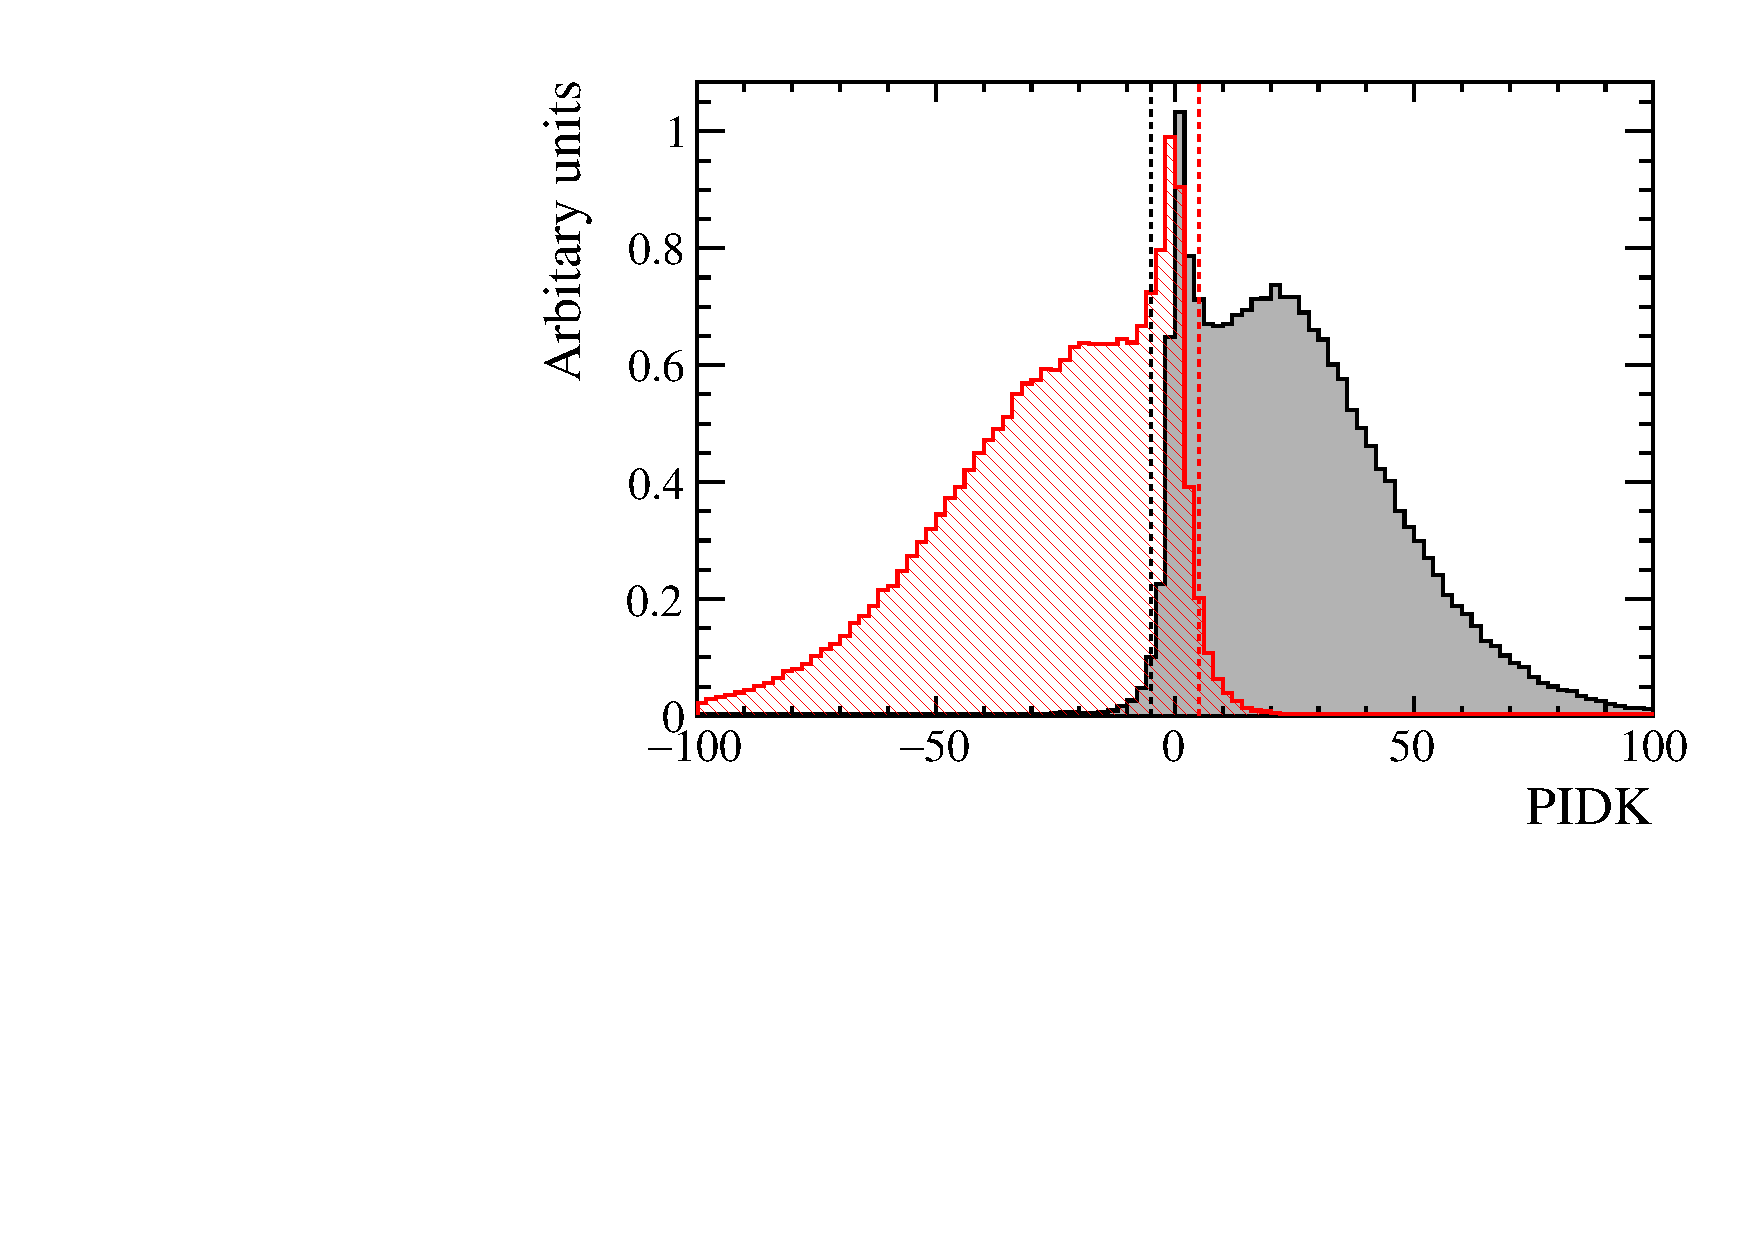
\includegraphics[width=0.6\textwidth]{figs/Selection/Calib_sample_PIDK.pdf}
        \caption{The distribution of the particle identification variable PIDK for pions (red) and kaons (black) from data calibration samples. The vertical dashed lines illustrate the requirements $\text{PIDK}<-5$ and $\text{PIDK}>5$ applied to pions and kaons respectively.}
    \label{fig:selection_PIDK_distribution}   
\end{figure}
%%%%%%%%%%%%%%%%%%%%%%%%%%%%%%%%%%%%%%%%%%%%%%%%%%%%%%%%%%

The kaons and pions originating from the decays of \Dsp mesons are required to pass $\text{PIDK} > -5$ and $\text{PIDK} < 5$ respectively. Kaons originating in the \phiz-meson decay, or from the \Bp meson in the case of \decay{\Bp}{\Dsp\Kp\Km}, are required to pass $\text{PIDK} > 0$. These requirements have a combined efficiency of between 85-90\%, depending on \Dsp decay mode. 



\subsection{Charmless and single-charm backgrounds}


Decays of \Bp mesons that didn't proceed via \D mesons could form a peaking background below the signal invariant mass distributions when they decay to the same final state.
The signal mode could receive contributions from the decays $\decay{\Bp}{h^{+}h^{-}h^{+}\phiz}$ or $\decay{\Bp}{h^{+}h^{-}h^{+}h^{+}h^{-}}$, referred to as charmless backgrounds. Here $h^{\pm}$ is used to represent \Kpm or \pipm in the specific \Dsp, \Dzb or \phiz final state.
The normalisation mode is also susceptible, however as it involves two charm mesons it could receive contributions from the decays $\decay{\Bp}{h^{+}h^{-}h^{+}\Dzb}$ or $\decay{\Bp}{\Dsp h^{+}h^{-}}$, referred to as single-charm backgrounds, and $\decay{\Bp}{h^{+}h^{-}h^{+} h^{+}h^{-}}$ referred to as a charmless background.
These backgrounds can be suppressed by requiring the \D-meson decay vertex to be displaced from the \Bp-meson decay vertex. Requirements of varying strength are applied to the significance of the vertex separation ($\chi^{2}_{\text{FD}}$), depending on the extend to which each mode is affected by these backgrounds. The distributions of the flight distance significance for \decay{\Bp}{(\decay{\Dsp}{\Kp\pim\pip})\phiz} signal decays and the charmless \decay{\Bp}{\Kp\pim\pip\phiz} decay is shown in Fig.~\ref{fig:Selection_FDCHI2}.

%%%%%%%%%%%%%%%%%%%%%%%%%%%%%%%%%%%%%%%%%%%%%%%%%%%%%%%%%%
\begin{figure}[!h]
    \centering
        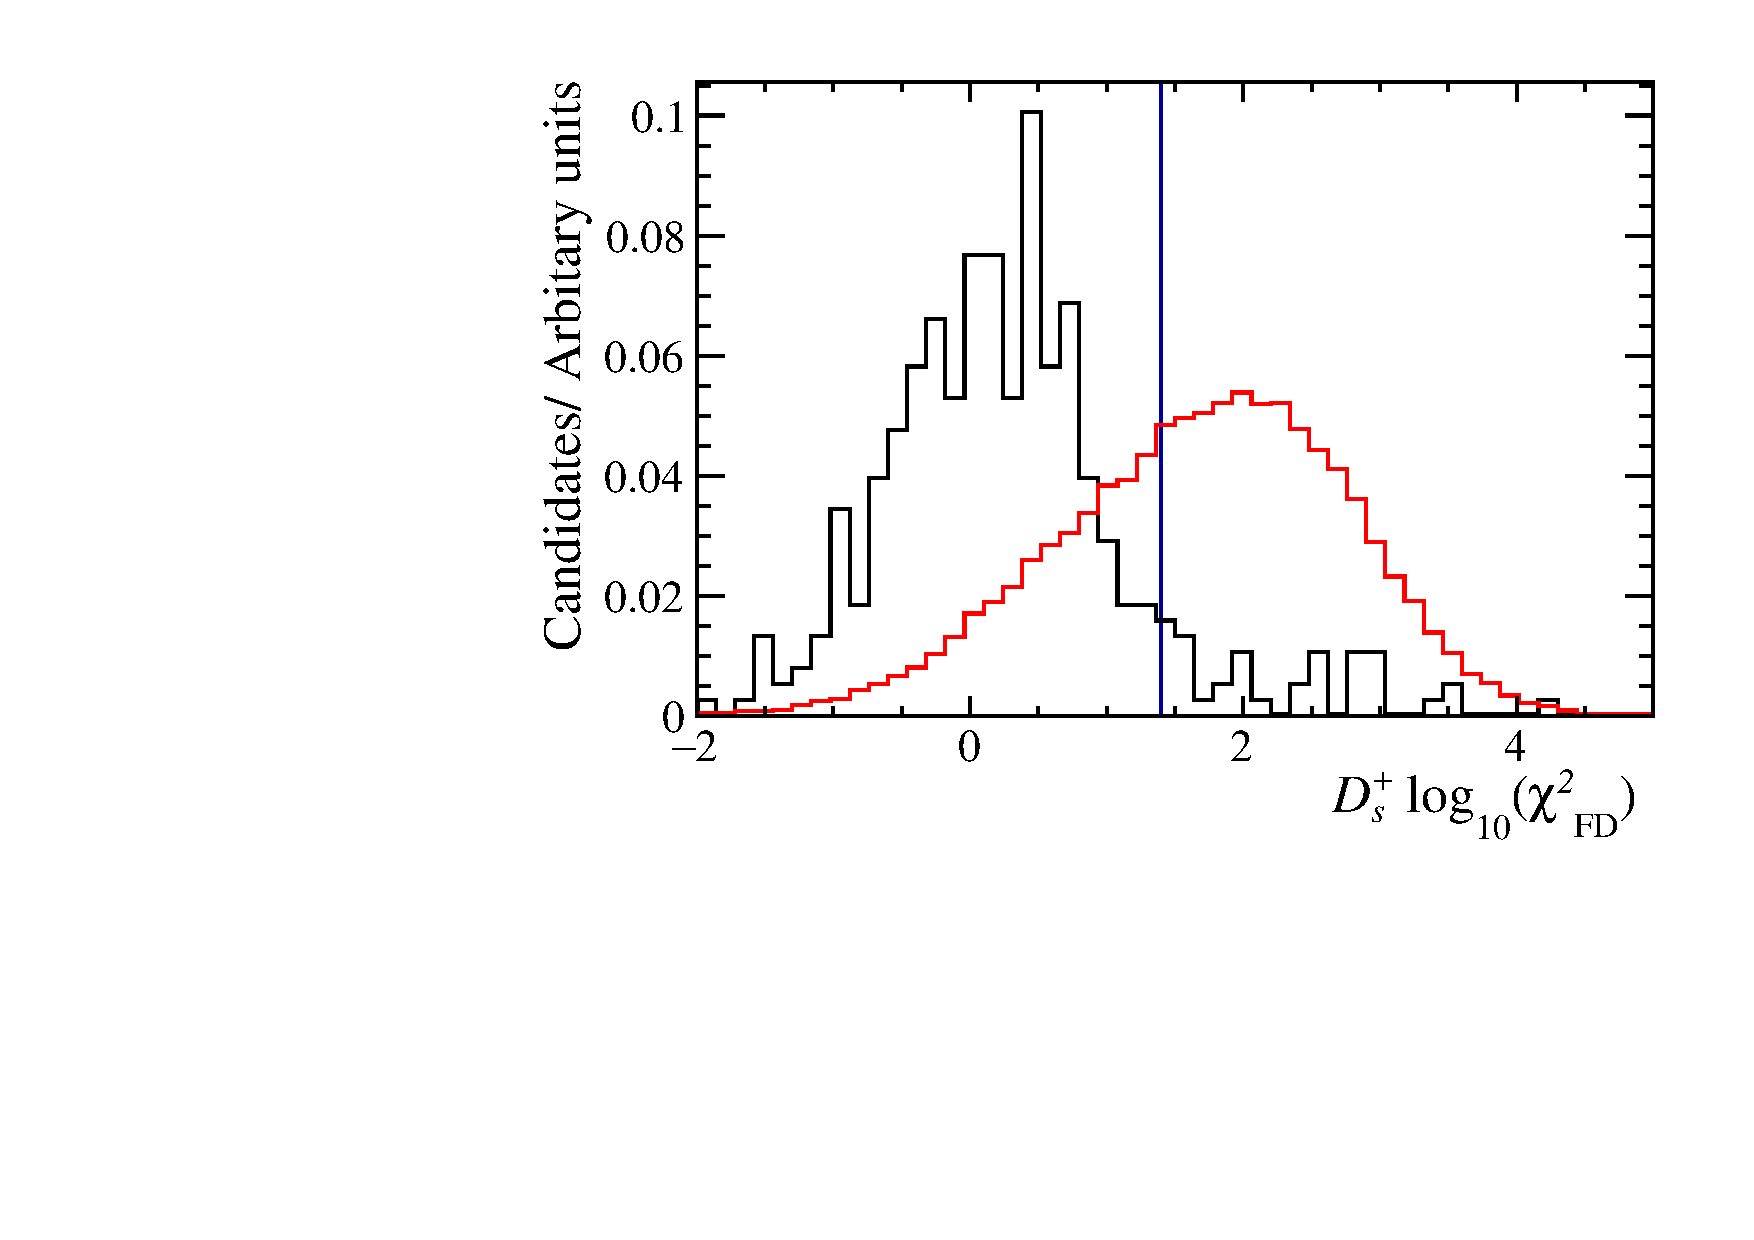
\includegraphics[width=0.6\textwidth]{figs/Selection/Charmless_Comparison_B2DsPhi_Ds2KPiPi_log10_D_FDCHI2_ORIVX.pdf}
        \caption{The log of the flight distance significance between the \Bp and \Dsp decay vertices in samples of charmless \decay{\Bp}{\Kp\pim\pip\phiz} decays in data (black) and \decay{\Bp}{(\decay{\Dsp}{\Kp\pim\pip})\phiz} signal decays in simulation (red). The vertical line represents the requirement applied to this mode. The charmless \decay{\Bp}{\Kp\pim\pip\phiz} sample is select by placing the requirement $|m(\Kp\pim\pim\phiz)-m(\Bp)|<60\mevcc$ on \decay{\Bp}{(\decay{\Dsp}{\Kp\pim\pip})\phiz} candidates with $25 < |m(\Kp\pim\pip) - m(\Dsp)| < 50\mevcc $.}
    \label{fig:Selection_FDCHI2}   
\end{figure}
%%%%%%%%%%%%%%%%%%%%%%%%%%%%%%%%%%%%%%%%%%%%%%%%%%%%%%%%%%

The residual yields of charmless backgrounds in the signal mode are estimated by performing a fit to the \Bp invariant mass for candidates with $25 < |m(h^{+}h^{-}h^{+}) - m(\Dsp)| < 50\mevcc $. This background estimation is performed separately for the \decay{\Bp}{\Dsp\phiz} and \decay{\Bp}{\Dsp\Kp\Km} searches. 
The invariant mass distribution for \decay{\Bp}{(\decay{\Dsp}{\Kp\pim\pip})\phiz} candidates with $25 < |m(\Kp\pim\pip) - m(\Dsp)| < 50\mevcc$ is shown in Fig.~\ref{fig:Selection_charmless_before_after}, with and without the flight distance significance requirement applied. The large contribution from charmless decays is effectively removed.
%%%%%%%%%%%%%%%%%%%%%%%%%%%%%%%%%%%%%%%%%%%%%%%%%%%%%%%%%%
\begin{figure}[!h]
    \centering
    \begin{subfigure}[t]{0.4\textwidth}
        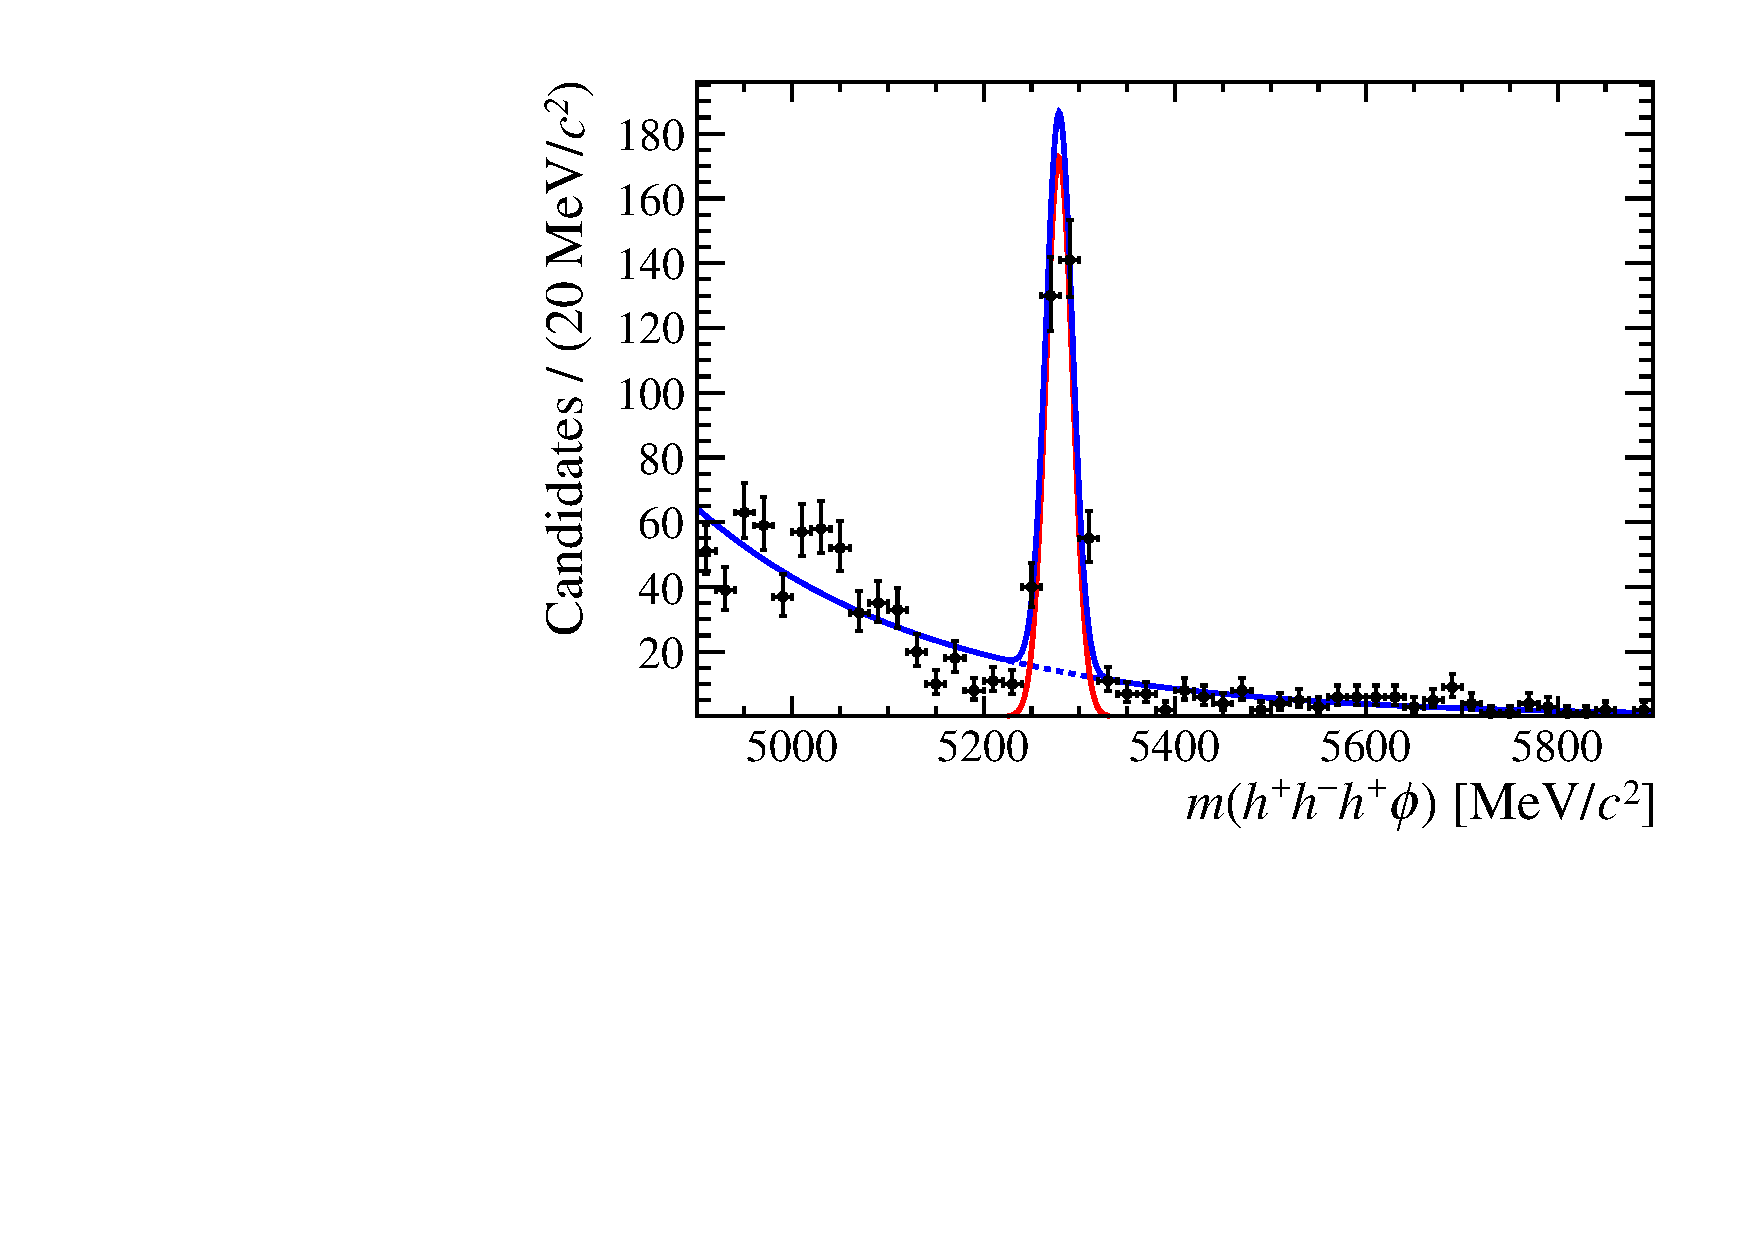
\includegraphics[width=1.0\textwidth]{figs/Selection/Signal_Ds2KPiPi_Test2_0_000000_DslessFDCHI2.pdf}
        \caption{Before}
    \end{subfigure}%
    \begin{subfigure}[t]{0.4\textwidth}
        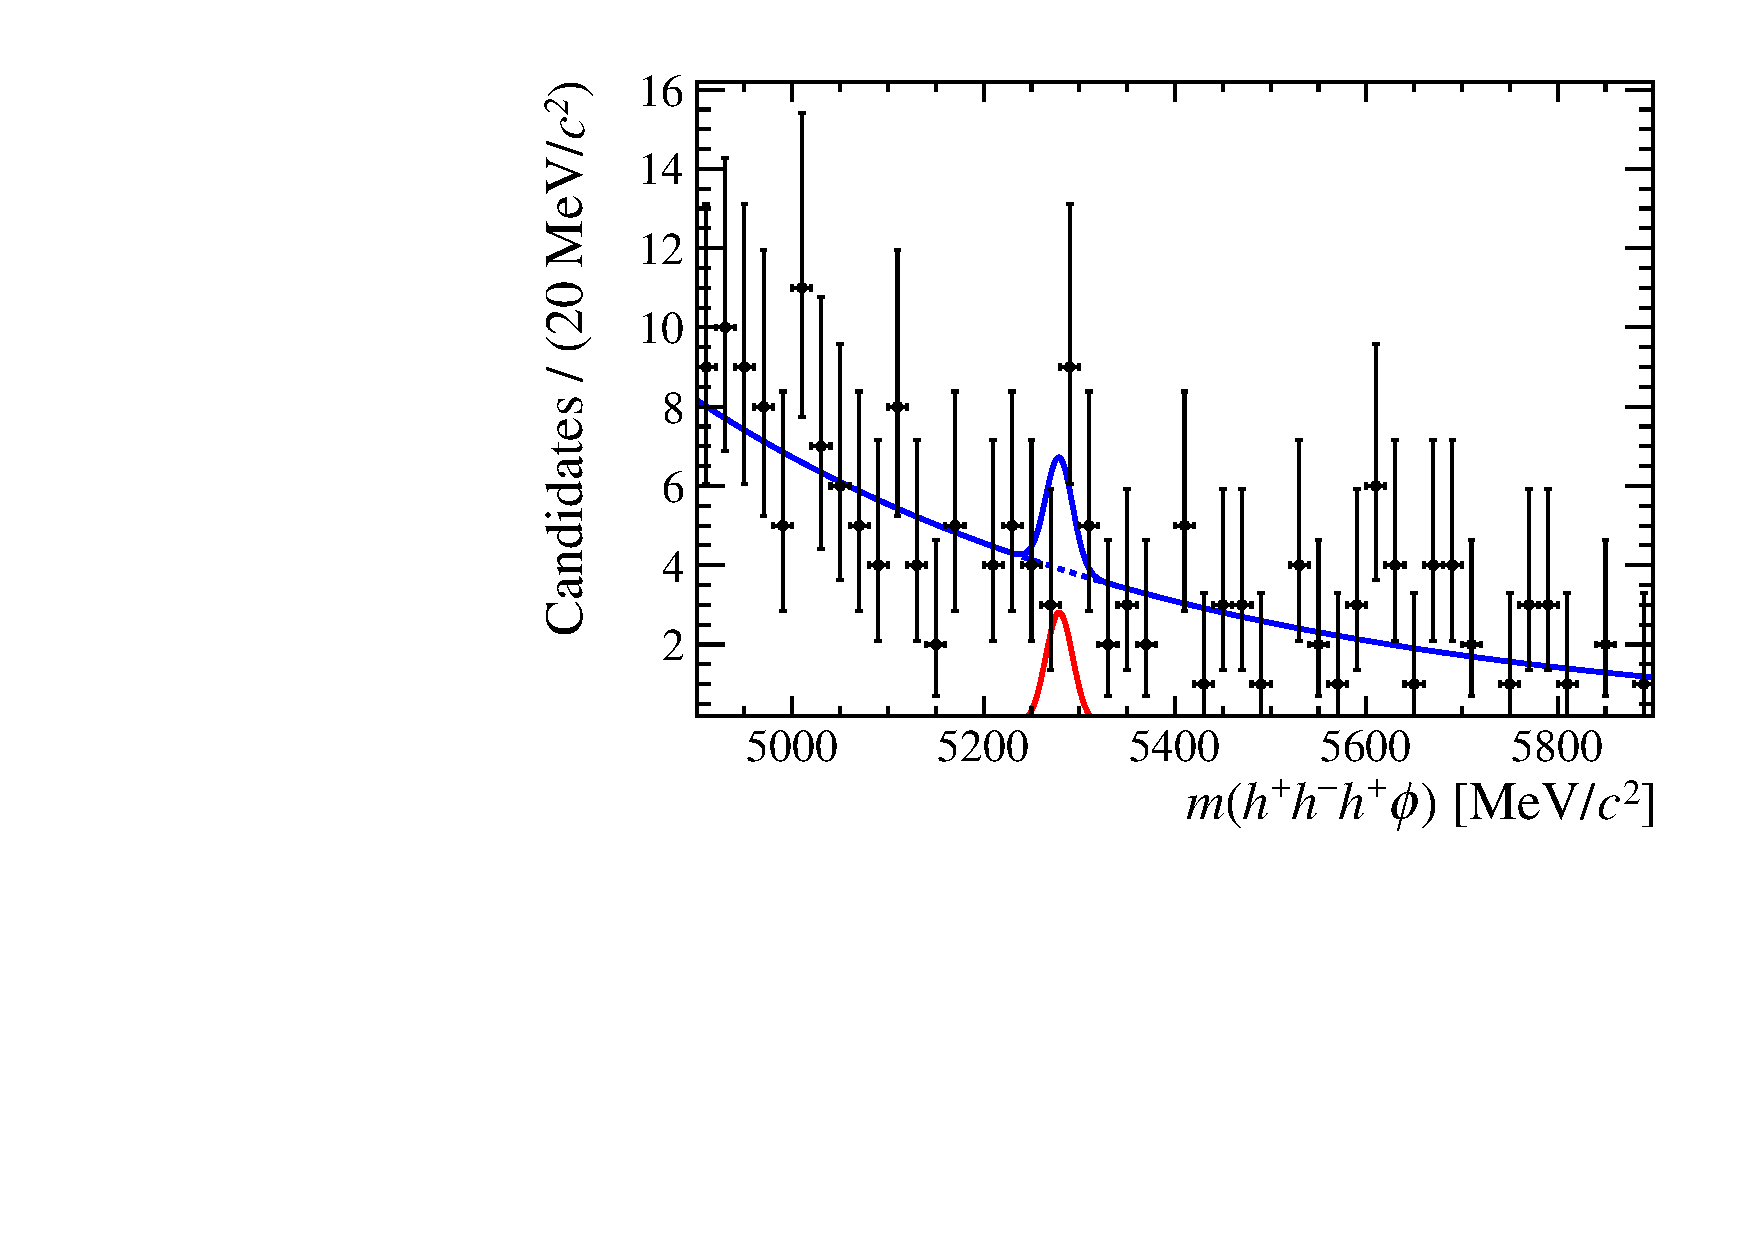
\includegraphics[width=1.0\textwidth]{figs/Selection/Signal_Ds2KPiPi_Test2_25_000000_DslessFDCHI2.pdf}
        \caption{After}
    \end{subfigure}\\
    \caption{The invariant mass distribution of \decay{\Bp}{(\decay{\Dsp}{\Kp\pim\pip})\phiz} candidates with $25 < |m(\Kp\pim\pip) - m(\Dsp)| < 50\mevcc $ before (left) and after (right) the flight distance significance requirement is applied. The significant contribution from \decay{\Bp}{\Kp\pim\pip\phiz} and \decay{\Bp}{\Kp\pim\pip\Kp\Km} decays is removed. Partially reconstructed charmless decays below the \Bp meson mass are neglected in the simple fit model.}
    \label{fig:Selection_charmless_before_after}   
\end{figure}
%%%%%%%%%%%%%%%%%%%%%%%%%%%%%%%%%%%%%%%%%%%%%%%%%%%%%%%%%%


For the \decay{\Bp}{\Dsp\Dzb} normalisation channel, a two-dimensional optimisation is performed to calculate the contribution from decays without a \Dsp meson, \Dzb meson or both. 
The two-dimensional space defined by the \Dsp and \Dzb masses is split into four types of area as shown in Fig~\ref{fig:2d_normalisation}.

%%%%%%%%%%%%%%%%%%%%%%%%%%%%%%%%%%%%%%%%%%%%%%%%%%%%%%%%%%
\begin{figure}[!h]
    \centering
        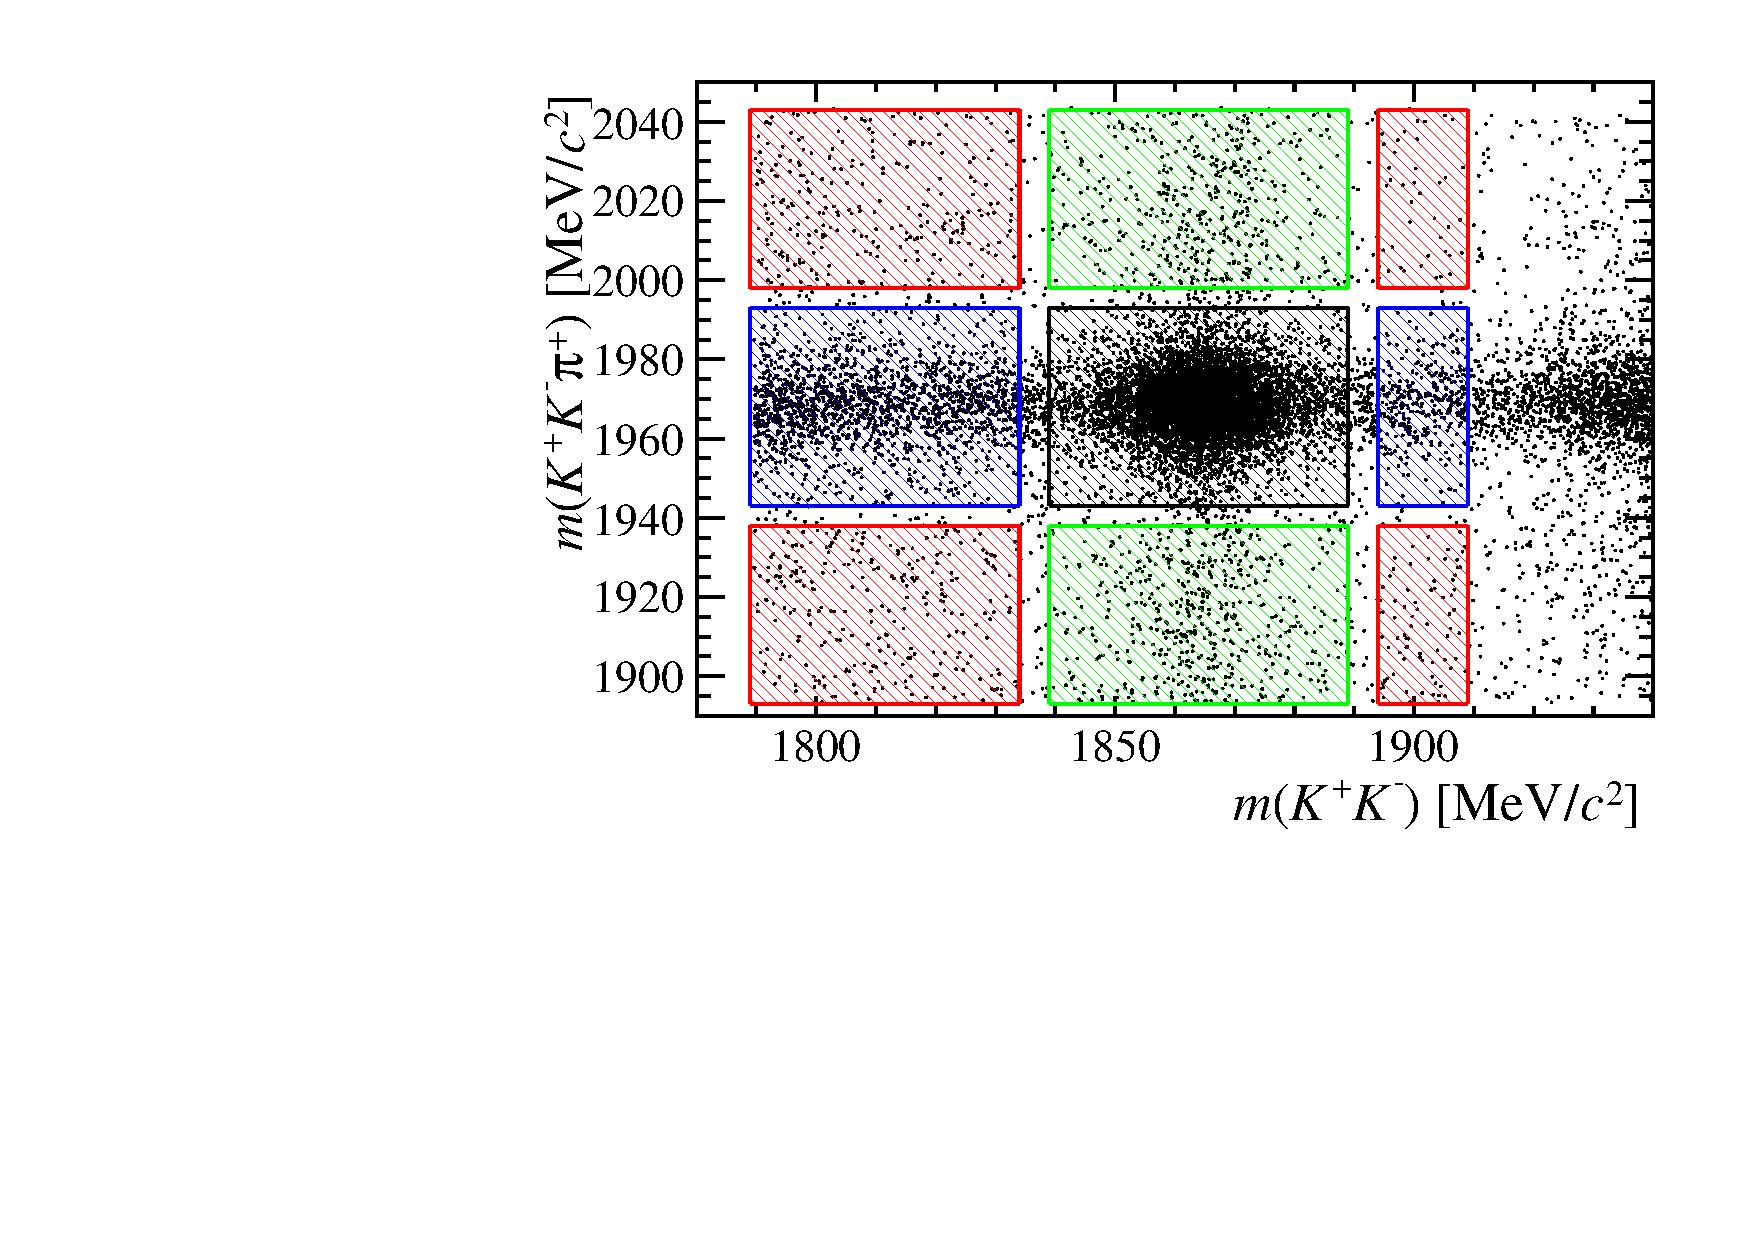
\includegraphics[width=0.6\textwidth]{figs/Selection/B2DsD0_2D_mass_Ds2KKPiRun2.pdf}
        \caption{Candidate \decay{\Bp}{\Dsp\Dzb} decays plotted as a function of the \Dsp and \Dzb invariant mass. The four regions described in the text are highlighted.}
    \label{fig:2d_normalisation}   
\end{figure}
%%%%%%%%%%%%%%%%%%%%%%%%%%%%%%%%%%%%%%%%%%%%%%%%%%%%%%%%%%

\begin{enumerate}
\item Areas in which only $\decay{\Bp}{h^{+}h^{-}h^{+}h^{+}h^{-}}$ decays contribute (red).
\item Areas in which either $\decay{\Bp}{D_{s}^{+}h^{+}h^{-}}$  or $\decay{\Bp}{h^{+}h^{-}h^{+} h^{+}h^{-}}$ decays can contribute (blue). 

\item Areas in which either $\decay{\Bp}{h^{+}h^{-}h^{+}\Dzb}$ or $\decay{\Bp}{h^{+}h^{-}h^{+} h^{+}h^{-}}$ decays can contribute (green). 
\item The signal region in which $\decay{\Bp}{D_{s}^{+} \Dzb}$, $\decay{\Bp}{h^{+}h^{-}h^{+}\Dzb}$, $\decay{\Bp}{D_{s}^{+}h^{+}h^{-}}$ or $\decay{\Bp}{h^{+}h^{-}h^{+}h^{+}h^{-}}$ decays could contribute (black).
\end{enumerate}   

As illustrated in Fig.~\ref{fig:2d_normalisation}, the blue and red regions in the \Dzb sidebands are wider to the left of the peak than the right. This helps to prevent misidentified \decay{\Bp}{\Dsp (\decay{\Dzb}{\Km\pip})} decays from being included in the sideband sample, visible as an excess of points at high values of $m(\Kp\Km)$.
The optimal selection requirements are chosen such that the maximal signal efficiency is achieved for a residual charmless contribution of $<2\%$ of the normalisation yield.

The optimisation of the signal and normalisation cuts is performed separately for each different \Dsp decay mode, and for the \decay{\Bp}{\Dsp\Kp\Km} and \decay{\Bp}{\Dsp\phiz} selections. The optimised requirements are listed in Table~\ref{tab:selection_fd_cuts}, along with the estimated residual yields of charmless and single charm yields in the signal region.  

\begin{table}[h]
   \centering
      \begin{tabular}{l c c c c }
         \hline
         \Bp decay mode         & \Dsp decay mode             & $\chi^{2}_{\text{FD}}(\Dsp)$  & $\chi^{2}_{\text{FD}}(\Dzb)$  & Residual yields \\ 
         \hline
         \decay{\Bp}{\Dsp\phiz} & \decay{\Dsp}{\Kp\Km\pip}    &  0.0              & -                 & 0.0             \\
         \decay{\Bp}{\Dsp\phiz} & \decay{\Dsp}{\Kp\pim\pip}   &  25.0             & -                 & 2.6             \\
         \decay{\Bp}{\Dsp\phiz} & \decay{\Dsp}{\pip\pim\pip}  &  5.0              & -                 & 0.0             \\
         \decay{\Bp}{\Dsp\Dzb}  & \decay{\Dsp}{\Kp\Km\pip}    &  8.0              & 0.0               & 21.6            \\
         \decay{\Bp}{\Dsp\Dzb}  & \decay{\Dsp}{\Kp\pim\pip}   &  18.0             & 0.0               & 3.3             \\
         \decay{\Bp}{\Dsp\Dzb}  & \decay{\Dsp}{\pip\pim\pip}  &  16.0             & 0.0               & 3.9             \\
         \hline
         \decay{\Bp}{\Dsp\Kp\Km} & \decay{\Dsp}{\Kp\Km\pip}   & 5.0               & -                 & 0.19            \\
         \decay{\Bp}{\Dsp\Dzb}   & \decay{\Dsp}{\Kp\Km\pip}   & 8.0               & 0.0               & 7.95            \\
         \hline
      \end{tabular}
   \caption{Charmless and single charm minimum flight distance significance requirements applied to the \Dsp and \Dzb candidates. The selection requirements are chosen such that the contribution from charmless and single charm decays are below 2\% of the normalisation yield. The large variation in residual yields therefore reflects reflects the variation in the expected normalisation yields.}
   \label{tab:selection_fd_cuts}
\end{table}




\subsection{Misidentified \D and \Lc hadrons}
\label{sec:pidvetos}

It is possible for the samples \Dsp mesons to be contaminated by other misidentified decays of \Dp mesons or \Lc baryons in which one of the decay products has been incorrectly identified.
Such backgrounds can be vetoed by recalculating the invariant mass of the \Dsp meson, swapping the mass hypothesis of the ambiguous track to that of the \kaon, \pion or \proton, depending on the decay mode. 
The particle identification requirements are tightened within a mass window around the \Dp or \Lc mass, effectively removing this crossfeed. For the mode \decay{\Dsp}{\Kp\Km\pip}, the vetoes are not applied to candidates for which $|m(\Km\Kp)-m_{\phiz}| < 10\mevcc$ as there are a high purity of \decay{\Dsp}{\Kp\Km\pip} decays in this region.

The specific vetoes included in this selection are listed in Table~\ref{table:pidvetos}. 
\begin{table*}[!ht]
\centering
\begin{tabular}{ l l l }
\hline
Decay Mode & Misidentified decay\\
\hline
\decay{\Dsp}{{\color{Red}\Kp}\Km\pip}   & \decay{\Dp}{{\color{Red}\pip}\Km\pip}    \\
                           & $\decay{\Lc}{{\color{Red}\Pp^{+}}\Km\pip}$     \\
%                           &                             \\
\hline
\decay{\Dsp}{{\color{Red}\Kp}\pim\pip}  & \decay{\Dp}{{\color{Red}\pip}\pim\pip}   \\
%                           &                             \\

\hline
\end{tabular}
\caption{Misidentified decays targeted by vetoes. The ambiguous track is highlighted in red in each case.}
\label{table:pidvetos}

\end{table*}
The invariant mass distributions for each the misidentified \decay{\Dsp}{\Kp\Km\pip} decays are shown in Figs.~\ref{fig:PIDVetos_Ds2KKPi_D_Veto} and \ref{fig:PIDVetos_Ds2KKPi_Lc_Veto}. For candidates within windows around the misidentified hadron mass, tighter PID requirements are imposed. These are illustrated in two-dimensional plots. 



% %%%%%%%%%%%%%%%%%%%%%%%%%%%%%%%%%%%%%%%%%%%%%%%%%%%%%%%%%%
% \begin{figure}[!h]
%     \centering
%     \begin{subfigure}[t]{0.4\textwidth}
%         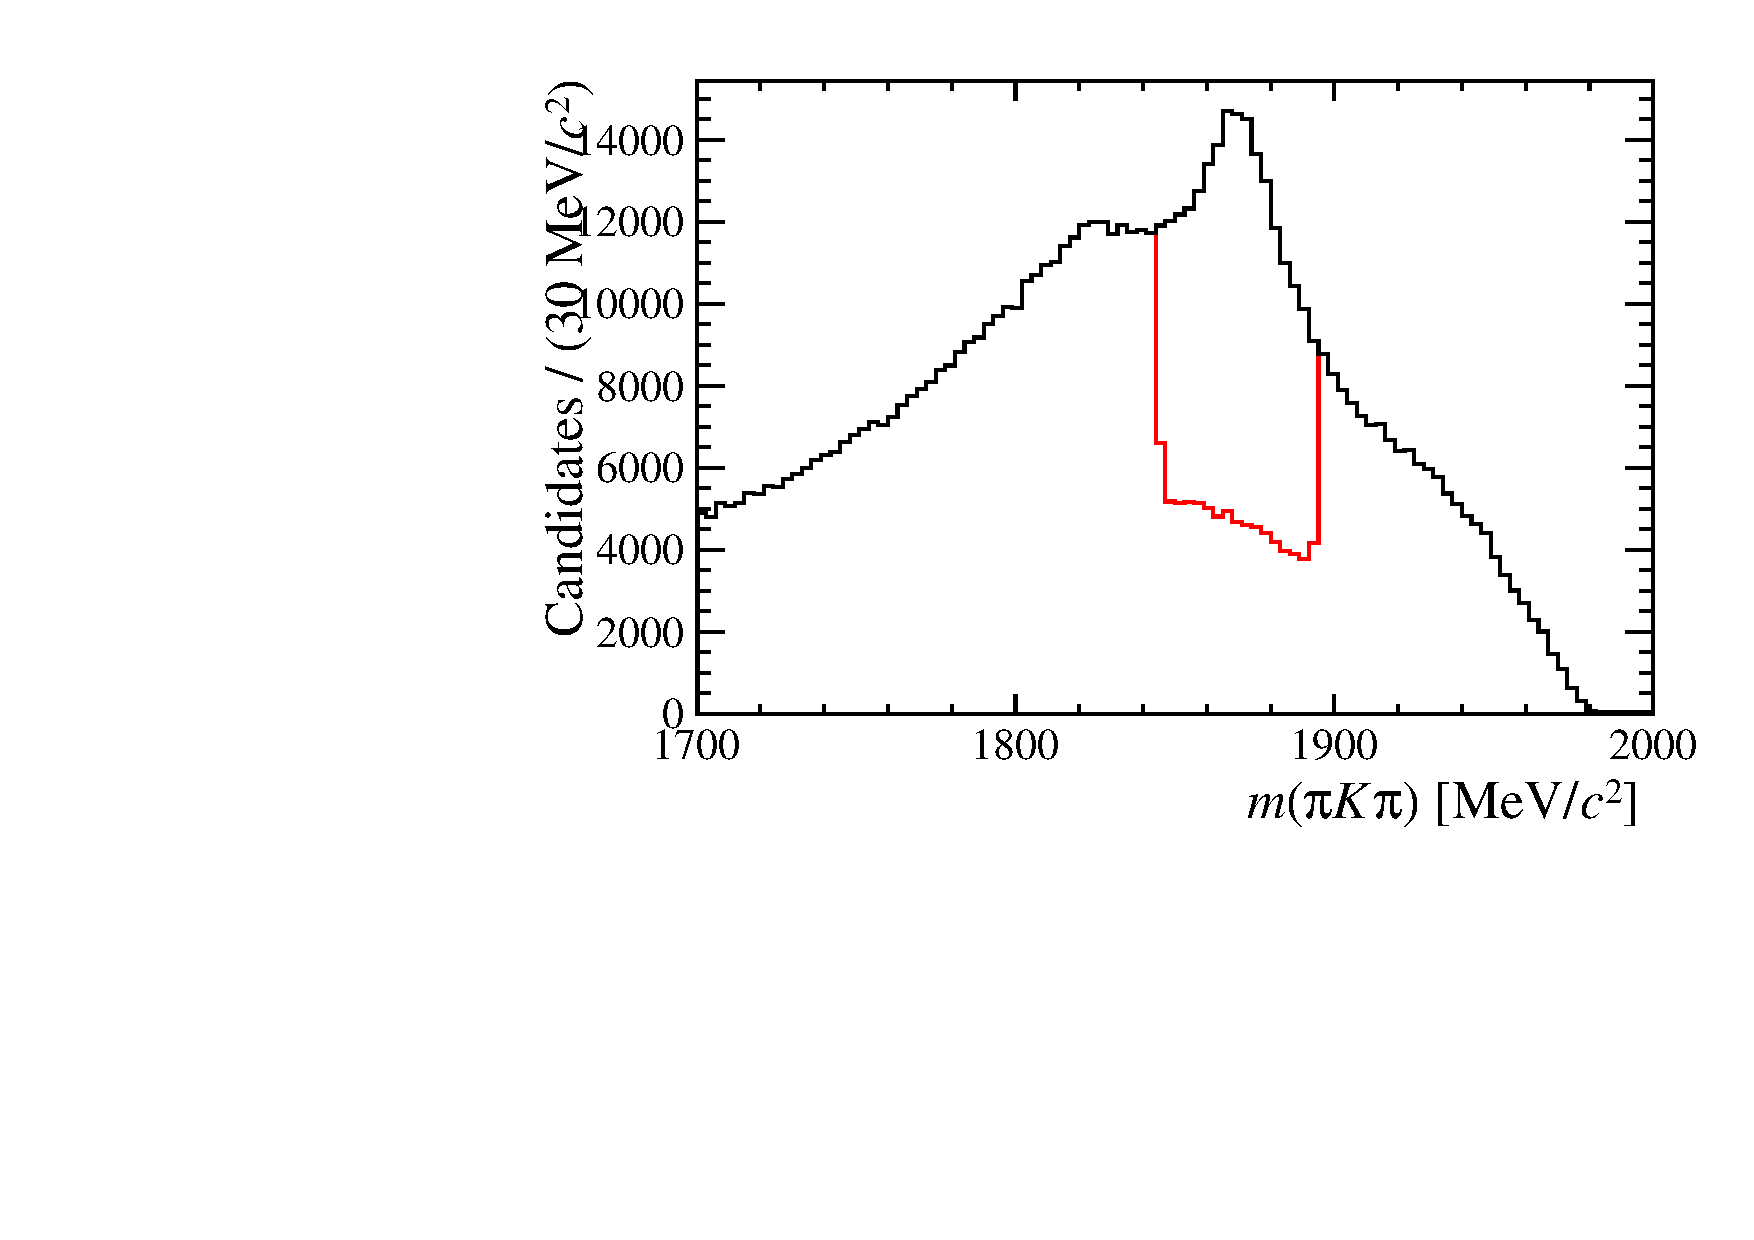
\includegraphics[width=1.0\textwidth]{figs/Selection/B2DsD0_Ds2KKPi_D_Veto_NoBDT.pdf}
%         \caption{Normalisation without selection}
%     \end{subfigure}%
%     \begin{subfigure}[t]{0.4\textwidth}
%         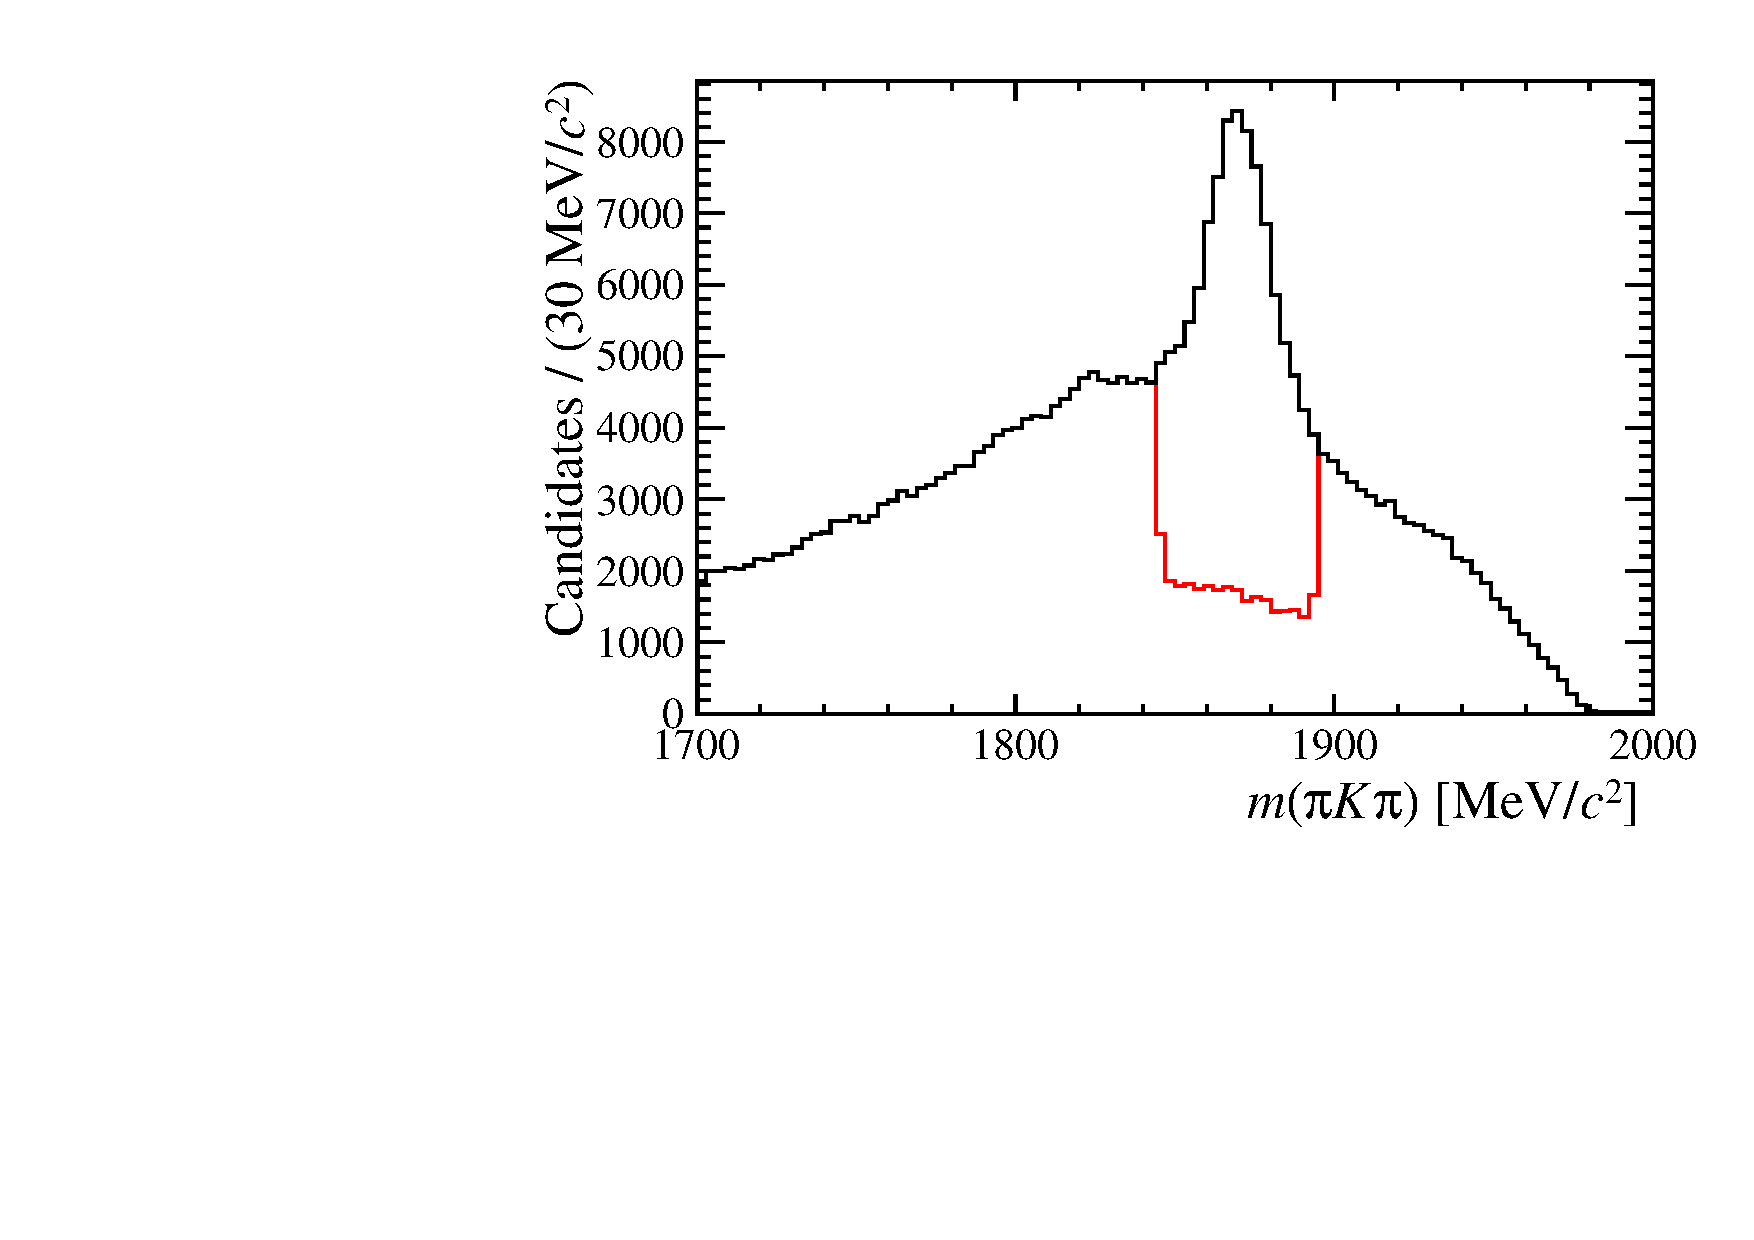
\includegraphics[width=1.0\textwidth]{figs/Selection/B2DsPhi_Ds2KKPi_D_Veto_NoBDT.pdf}
%         \caption{Signal without selection}
%     \end{subfigure}\\
%     \begin{subfigure}[t]{0.4\textwidth}
%         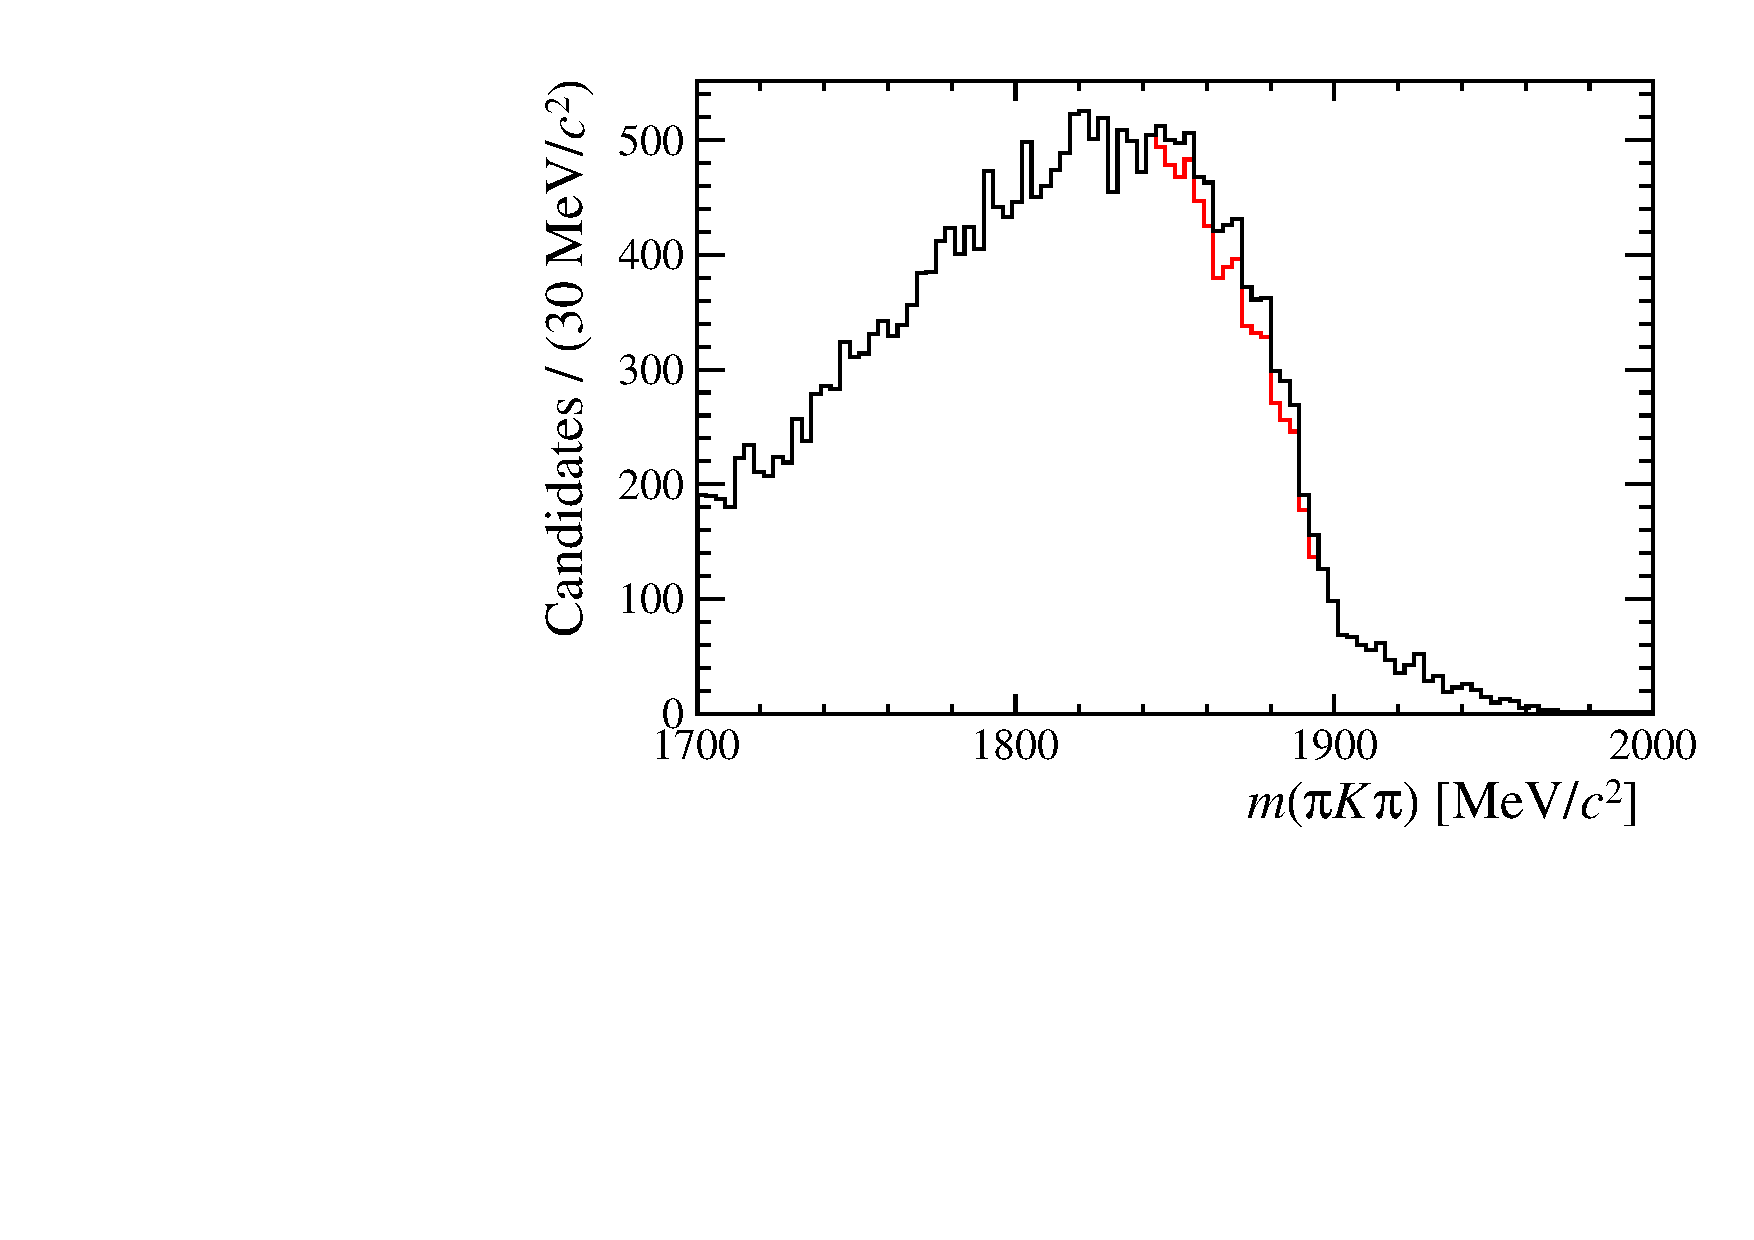
\includegraphics[width=1.0\textwidth]{figs/Selection/B2DsD0_Ds2KKPi_D_Veto_WithBDT.pdf}
%         \caption{Normalisation with selection}
%     \end{subfigure}%
%     \begin{subfigure}[t]{0.4\textwidth}
%         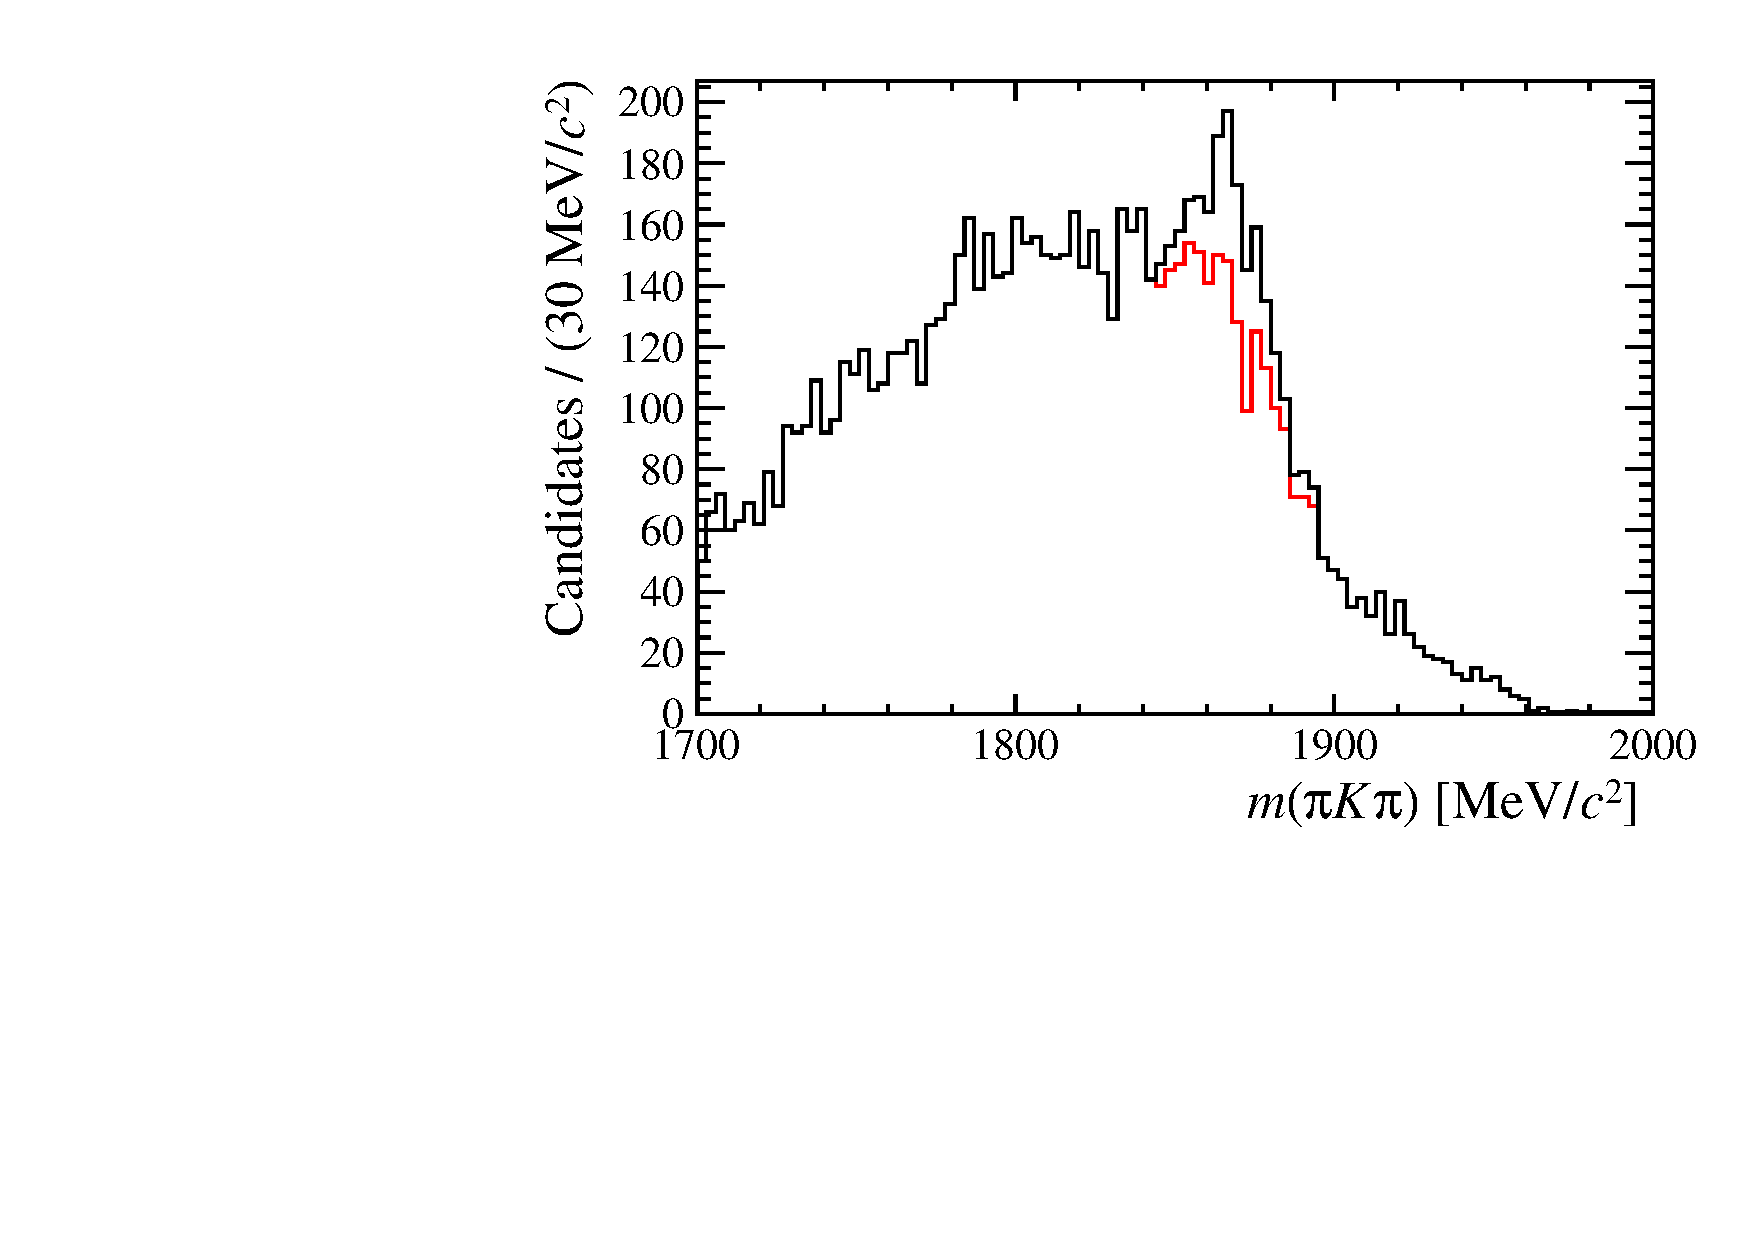
\includegraphics[width=1.0\textwidth]{figs/Selection/B2DsPhi_Ds2KKPi_D_Veto_WithBDT.pdf}
%         \caption{Signal with selection}
%     \end{subfigure}\\
%     \caption{Invariant mass distributions of \decay{\Dsp}{\Kp\Km\pip} samples reconstructed as \decay{\Dp}{\pip\Km\pip} for the signal and normalisation samples. The samples are shown with (red) and without (black) the veto described in Sec.~\ref{sec:pidvetos}. The distributions are shown before (top) and after (bottom) the MVA requirements have been applied.}
%     \label{fig:PIDVetos_Ds2KKPi_D_Veto}   
% \end{figure}
% %%%%%%%%%%%%%%%%%%%%%%%%%%%%%%%%%%%%%%%%%%%%%%%%%%%%%%%%%%


%%%%%%%%%%%%%%%%%%%%%%%%%%%%%%%%%%%%%%%%%%%%%%%%%%%%%%%%%%
\begin{figure}[!h]
    \centering
    \begin{subfigure}[t]{0.49\textwidth}
        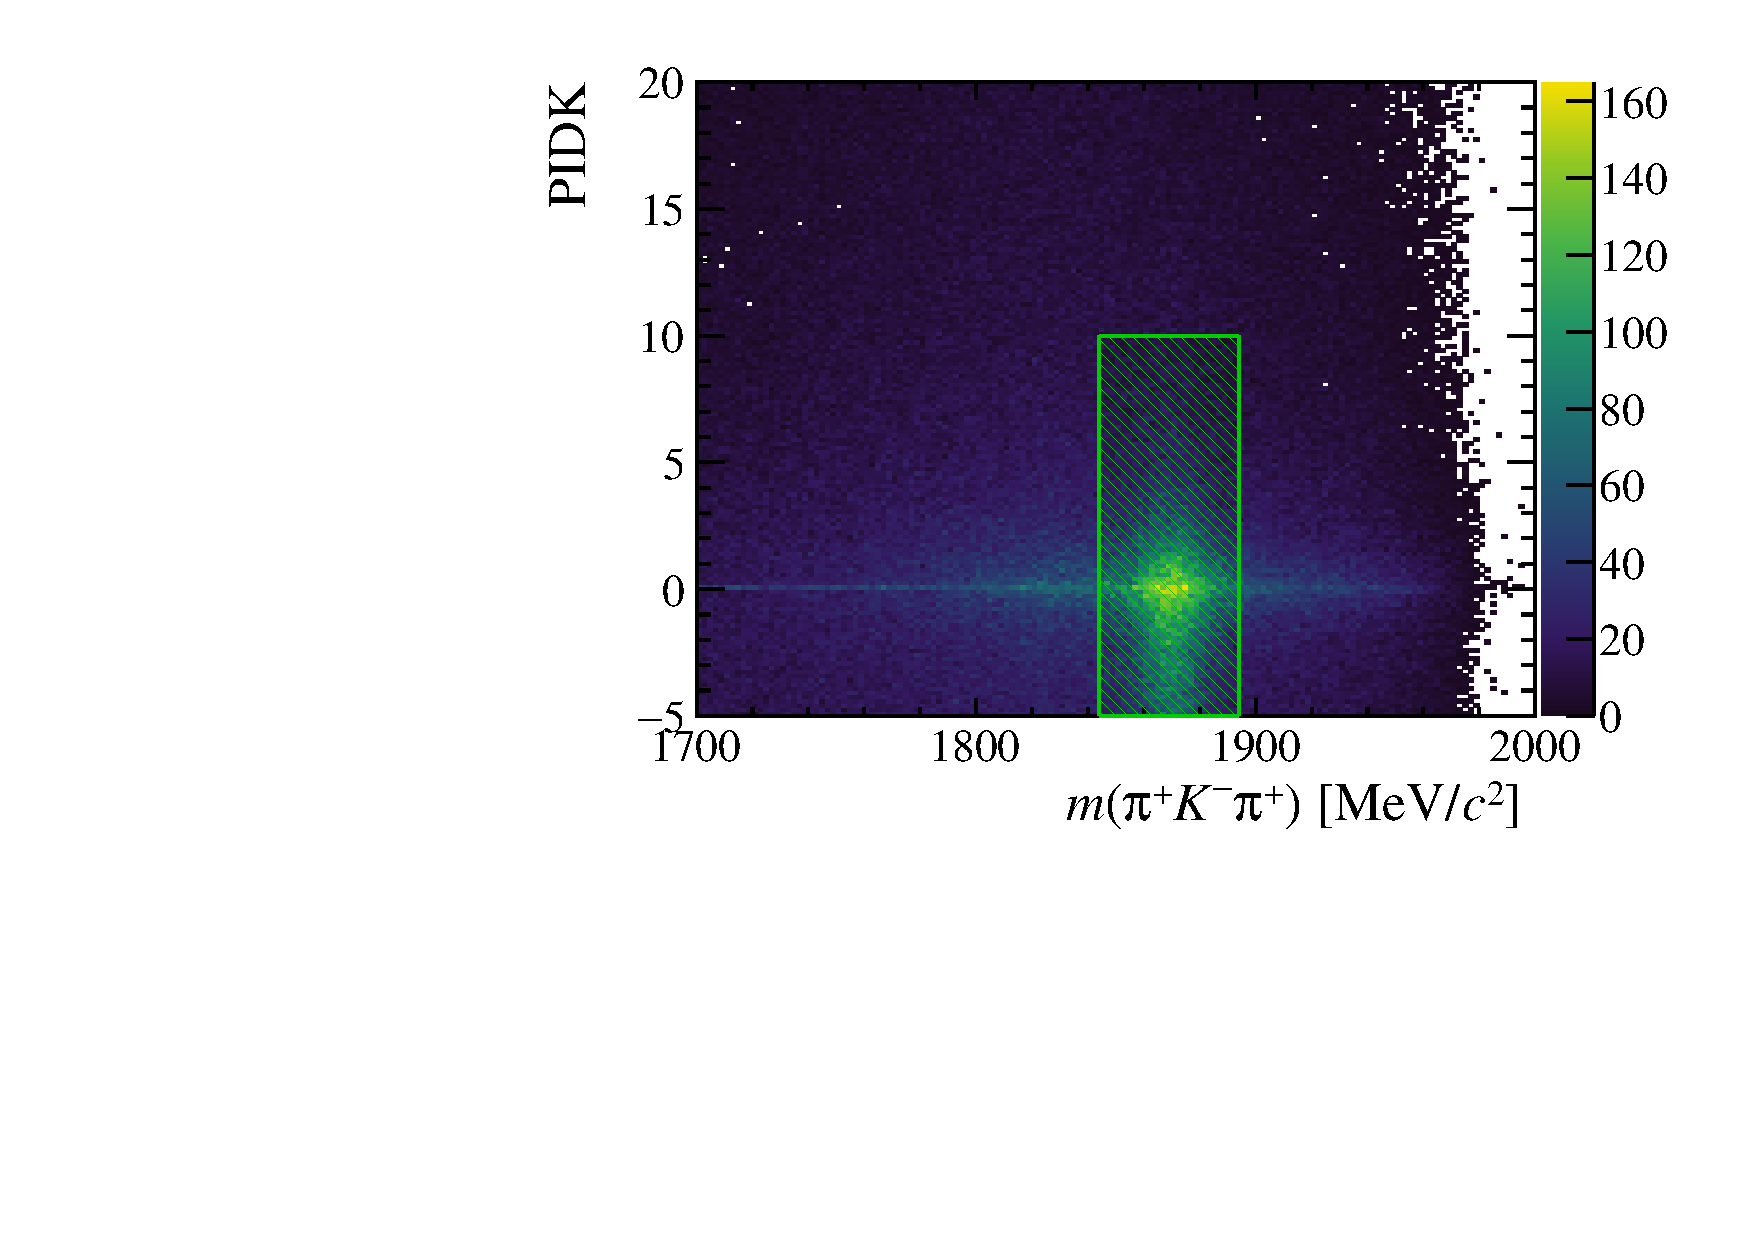
\includegraphics[width=1.0\textwidth]{figs/Selection/B2DsPhi_Ds2KKPi_2D_D_Veto_NoBDT.pdf}
        %\caption{Normalisation without selection}
    \end{subfigure}%
    \begin{subfigure}[t]{0.49\textwidth}
        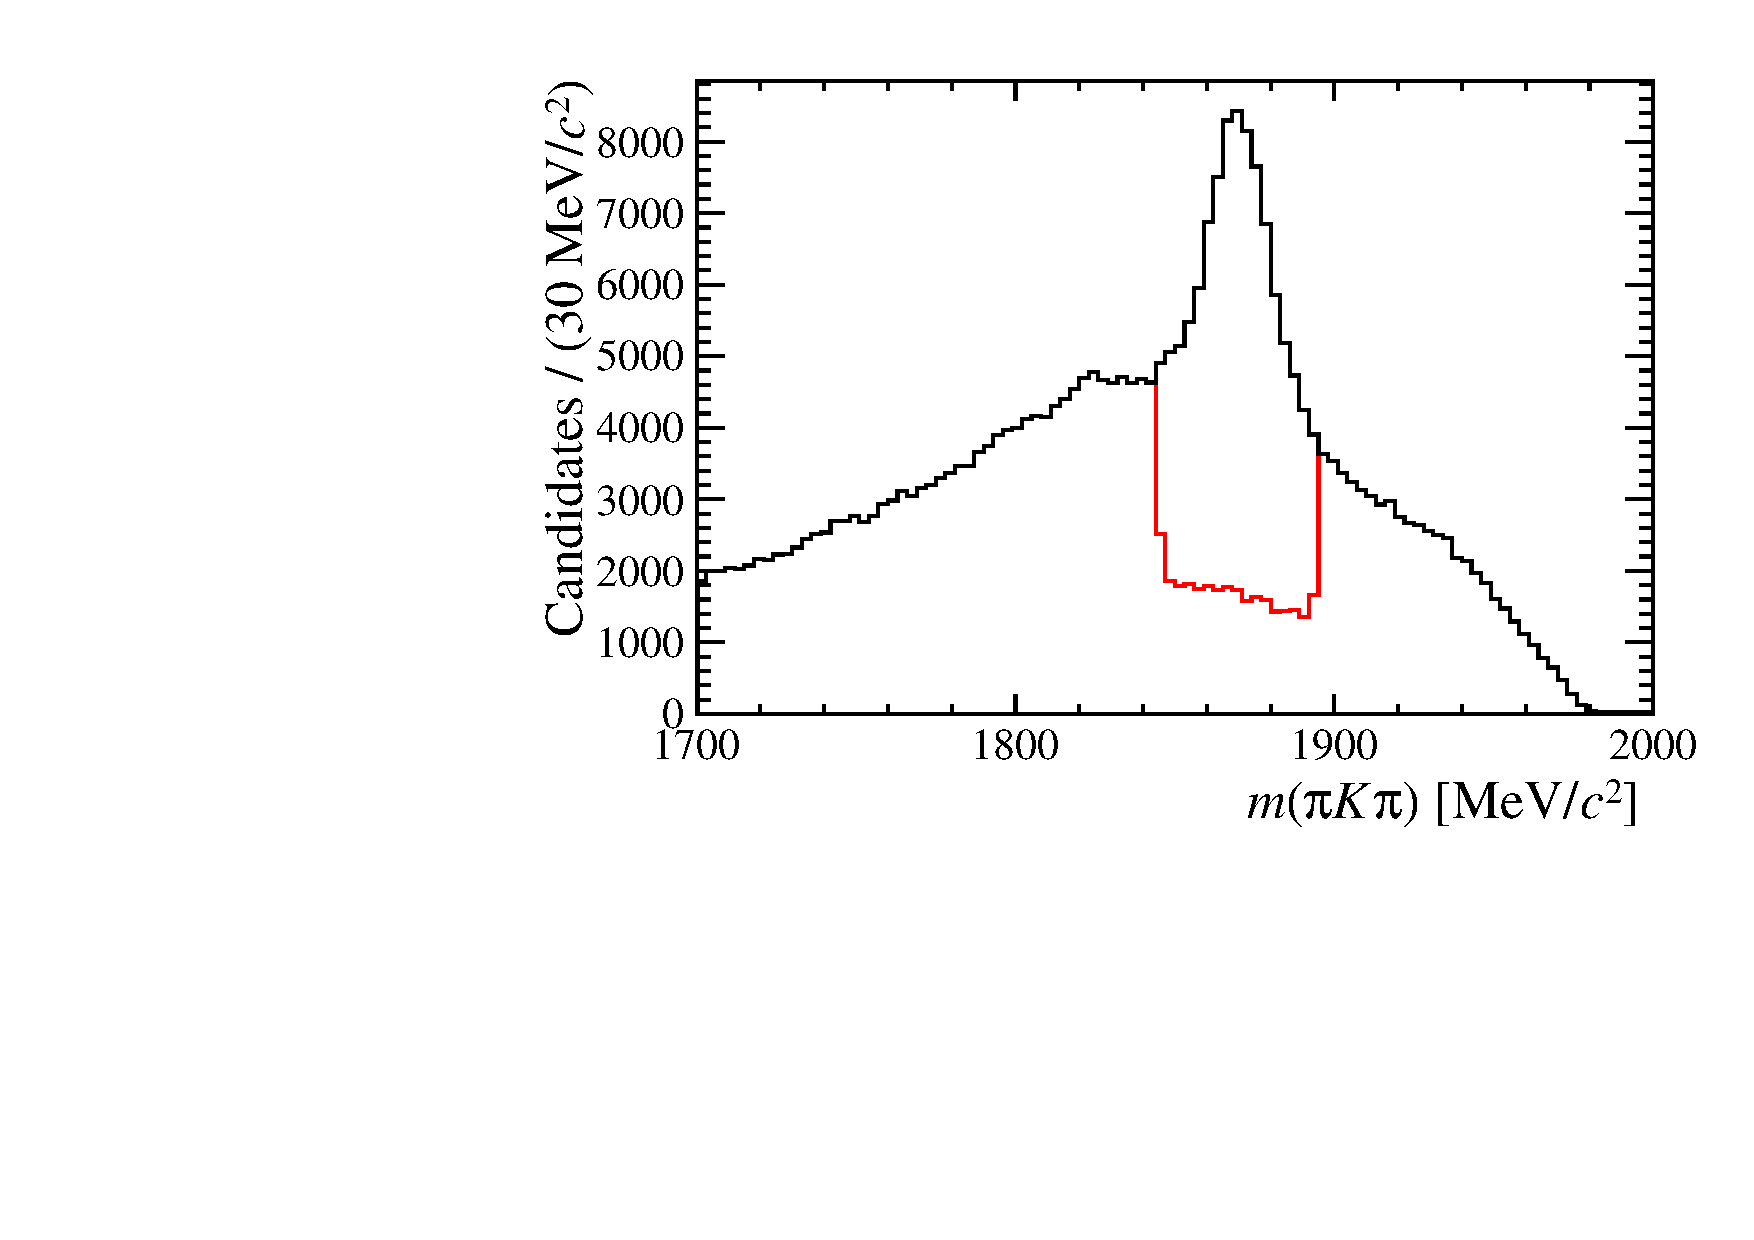
\includegraphics[width=1.0\textwidth]{figs/Selection/B2DsPhi_Ds2KKPi_D_Veto_NoBDT.pdf}
        %\caption{Signal without selection}
    \end{subfigure}\\
    \caption{The invariant mass distributions of \decay{\Dsp}{\Kp\Km\pip} samples reconstructed as \decay{\Dp}{\pip\Km\pip} plotted against the particle identification variable PIDK of the \Kp track (left). The green box represents the area removed by the veto. The misidentified invariant mass distribution (right) is plotted with (red) and without (black) the veto applied.}
    \label{fig:PIDVetos_Ds2KKPi_D_Veto}   
\end{figure}
%%%%%%%%%%%%%%%%%%%%%%%%%%%%%%%%%%%%%%%%%%%%%%%%%%%%%%%%%%

% %%%%%%%%%%%%%%%%%%%%%%%%%%%%%%%%%%%%%%%%%%%%%%%%%%%%%%%%%%
% \begin{figure}[!h]
%     \centering
%     \begin{subfigure}[t]{0.4\textwidth}
%         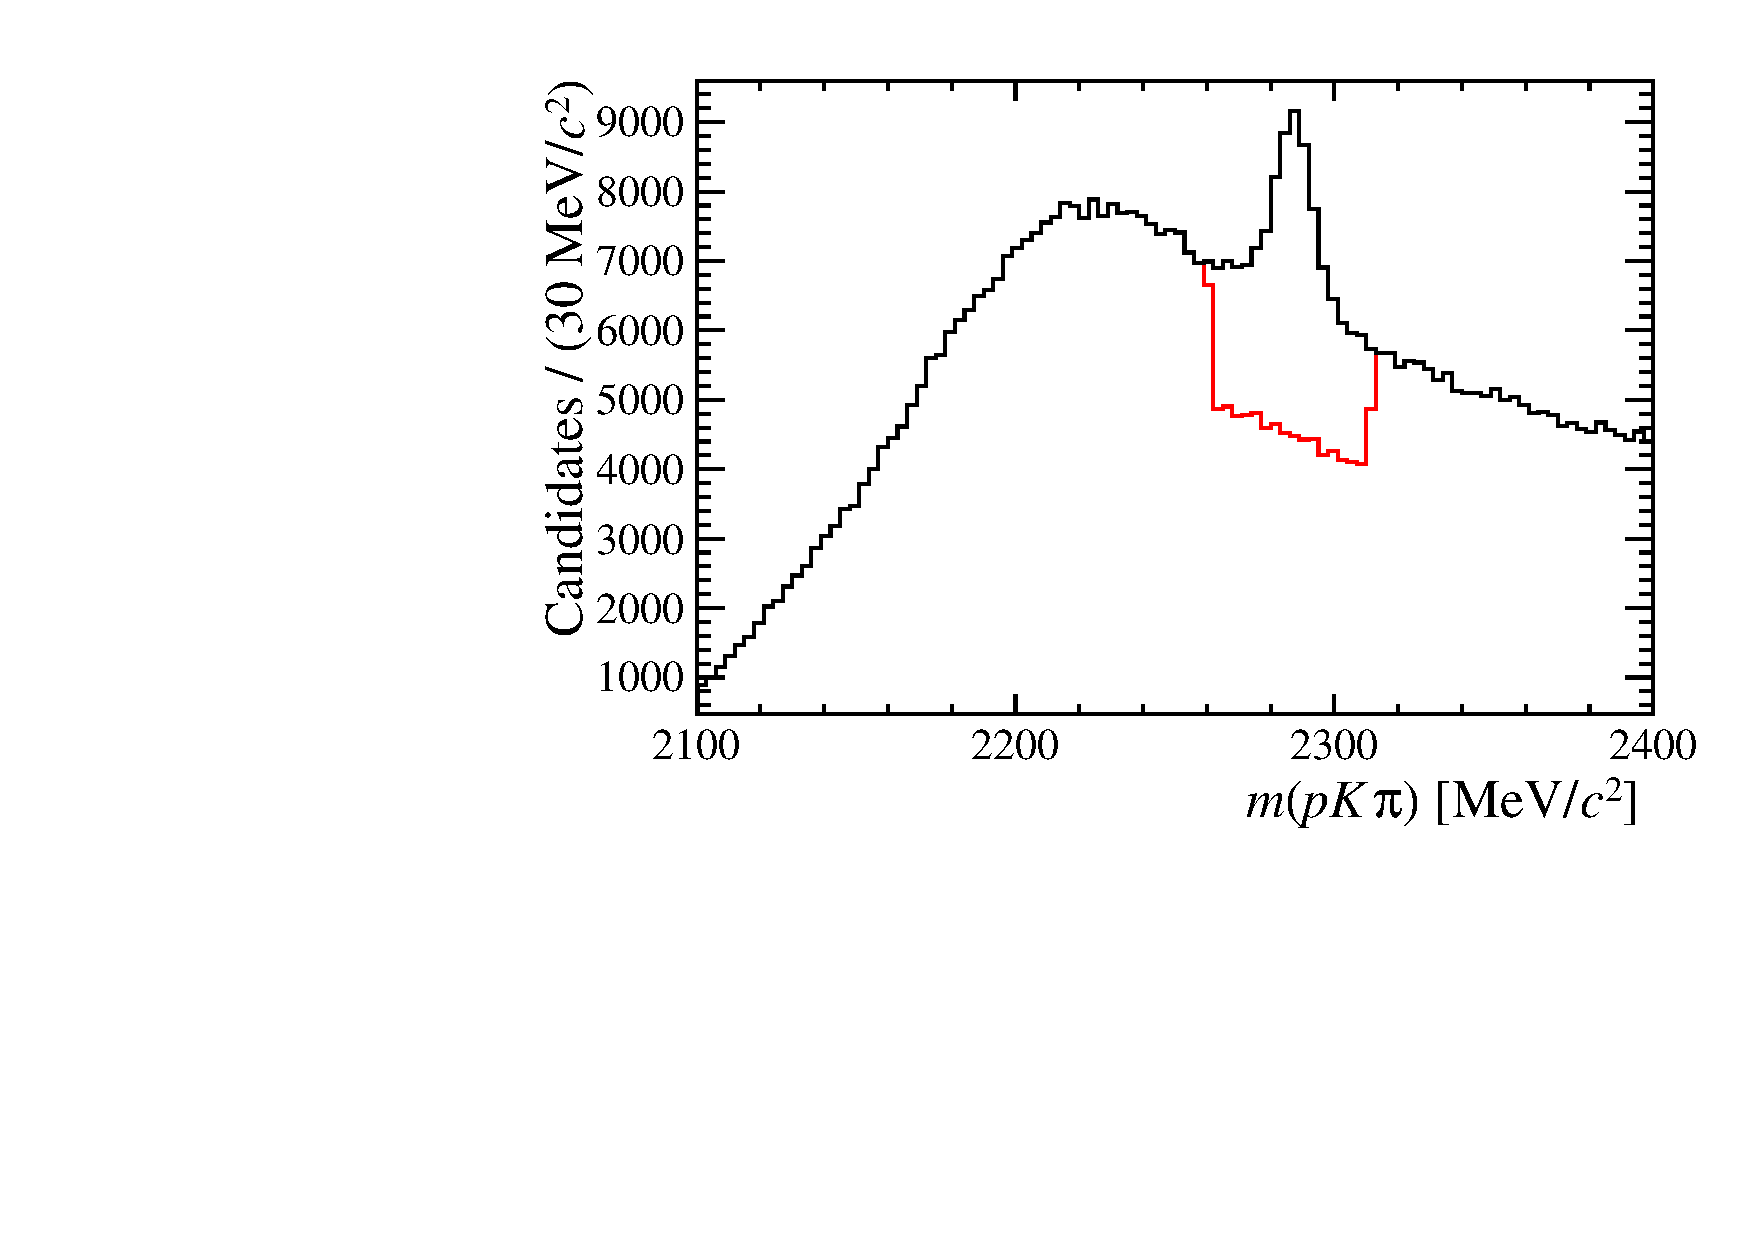
\includegraphics[width=1.0\textwidth]{figs/Selection/B2DsD0_Ds2KKPi_Lc_Veto_NoBDT.pdf}
%         \caption{Normalisation without MVA cut}
%     \end{subfigure}%
%     \begin{subfigure}[t]{0.4\textwidth}
%         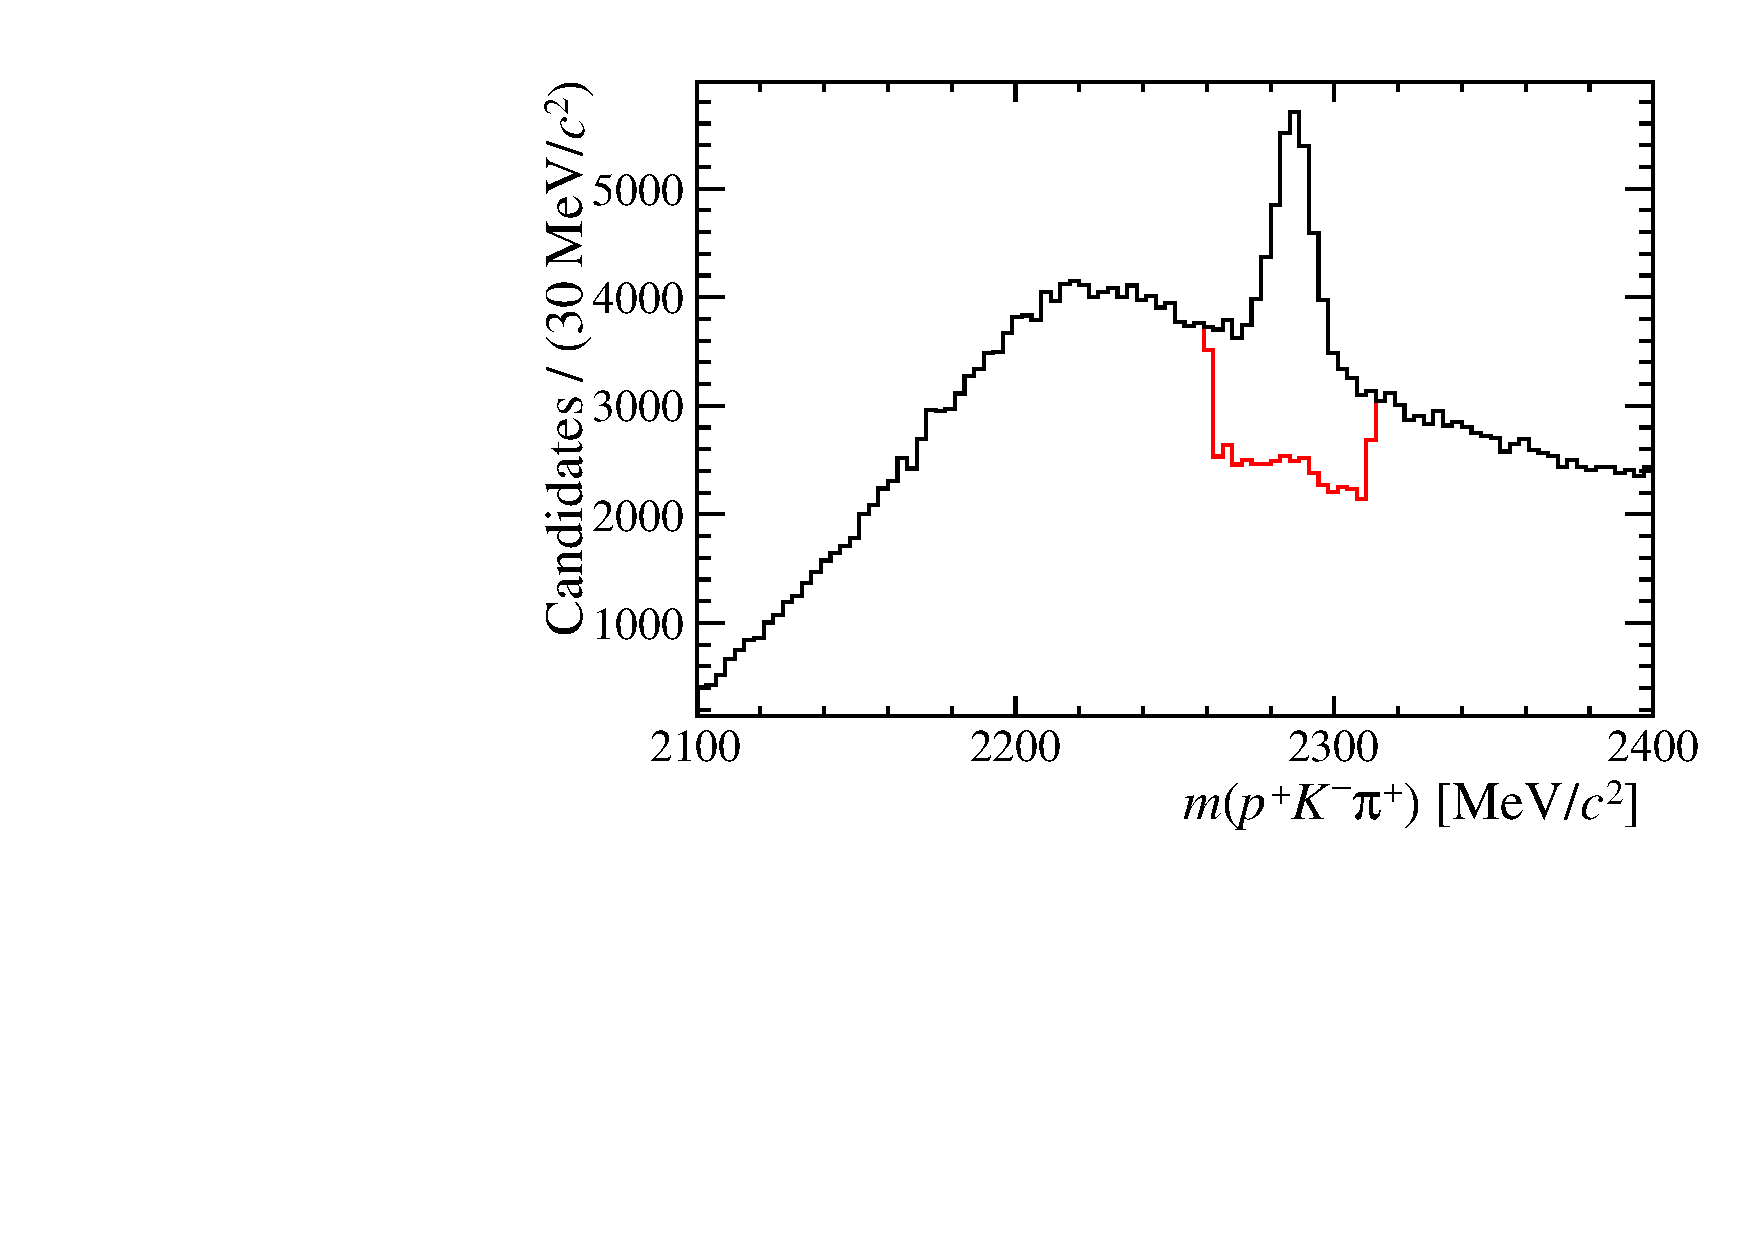
\includegraphics[width=1.0\textwidth]{figs/Selection/B2DsPhi_Ds2KKPi_Lc_Veto_NoBDT.pdf}
%         \caption{Signal without MVA cut}
%     \end{subfigure}\\
%     \begin{subfigure}[t]{0.4\textwidth}
%         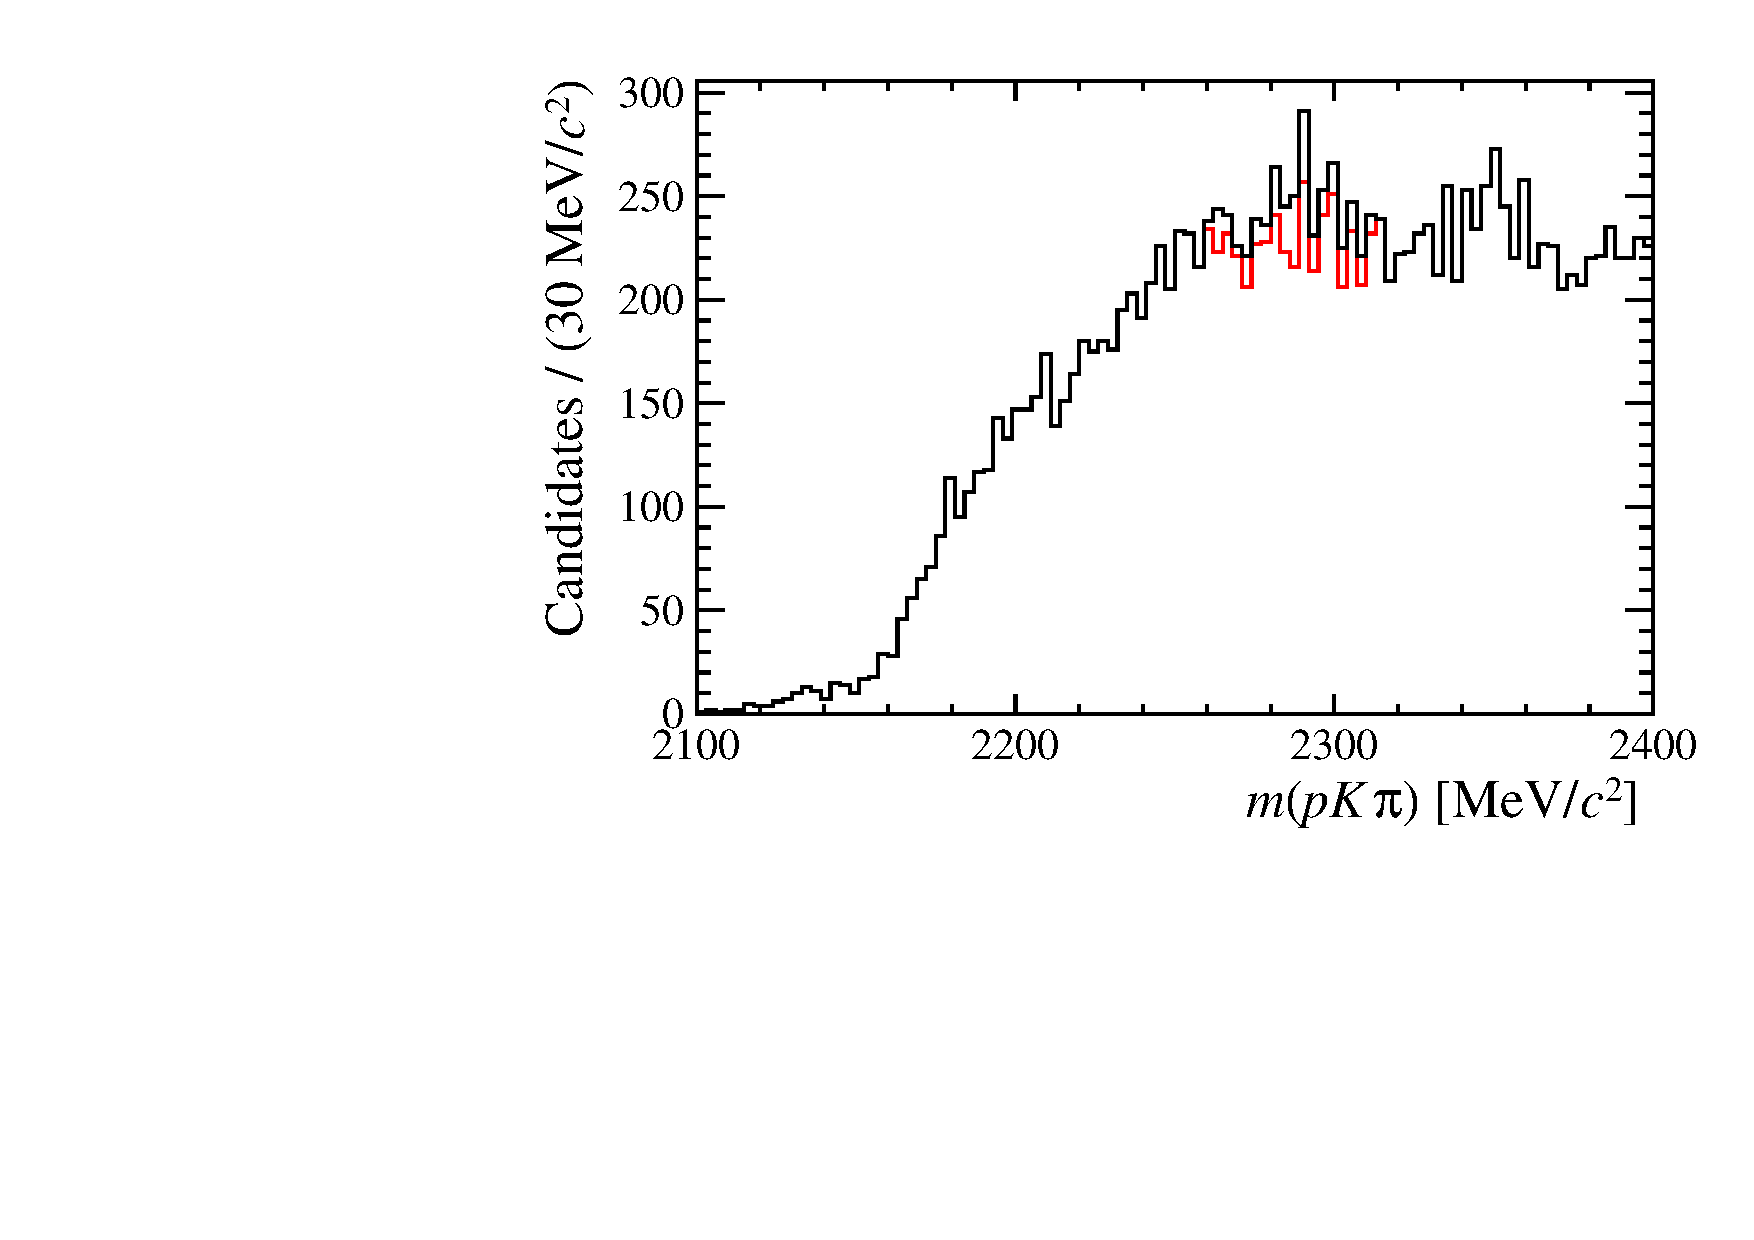
\includegraphics[width=1.0\textwidth]{figs/Selection/B2DsD0_Ds2KKPi_Lc_Veto_WithBDT.pdf}
%         \caption{Normalisation with MVA cut}
%     \end{subfigure}%
%     \begin{subfigure}[t]{0.4\textwidth}
%         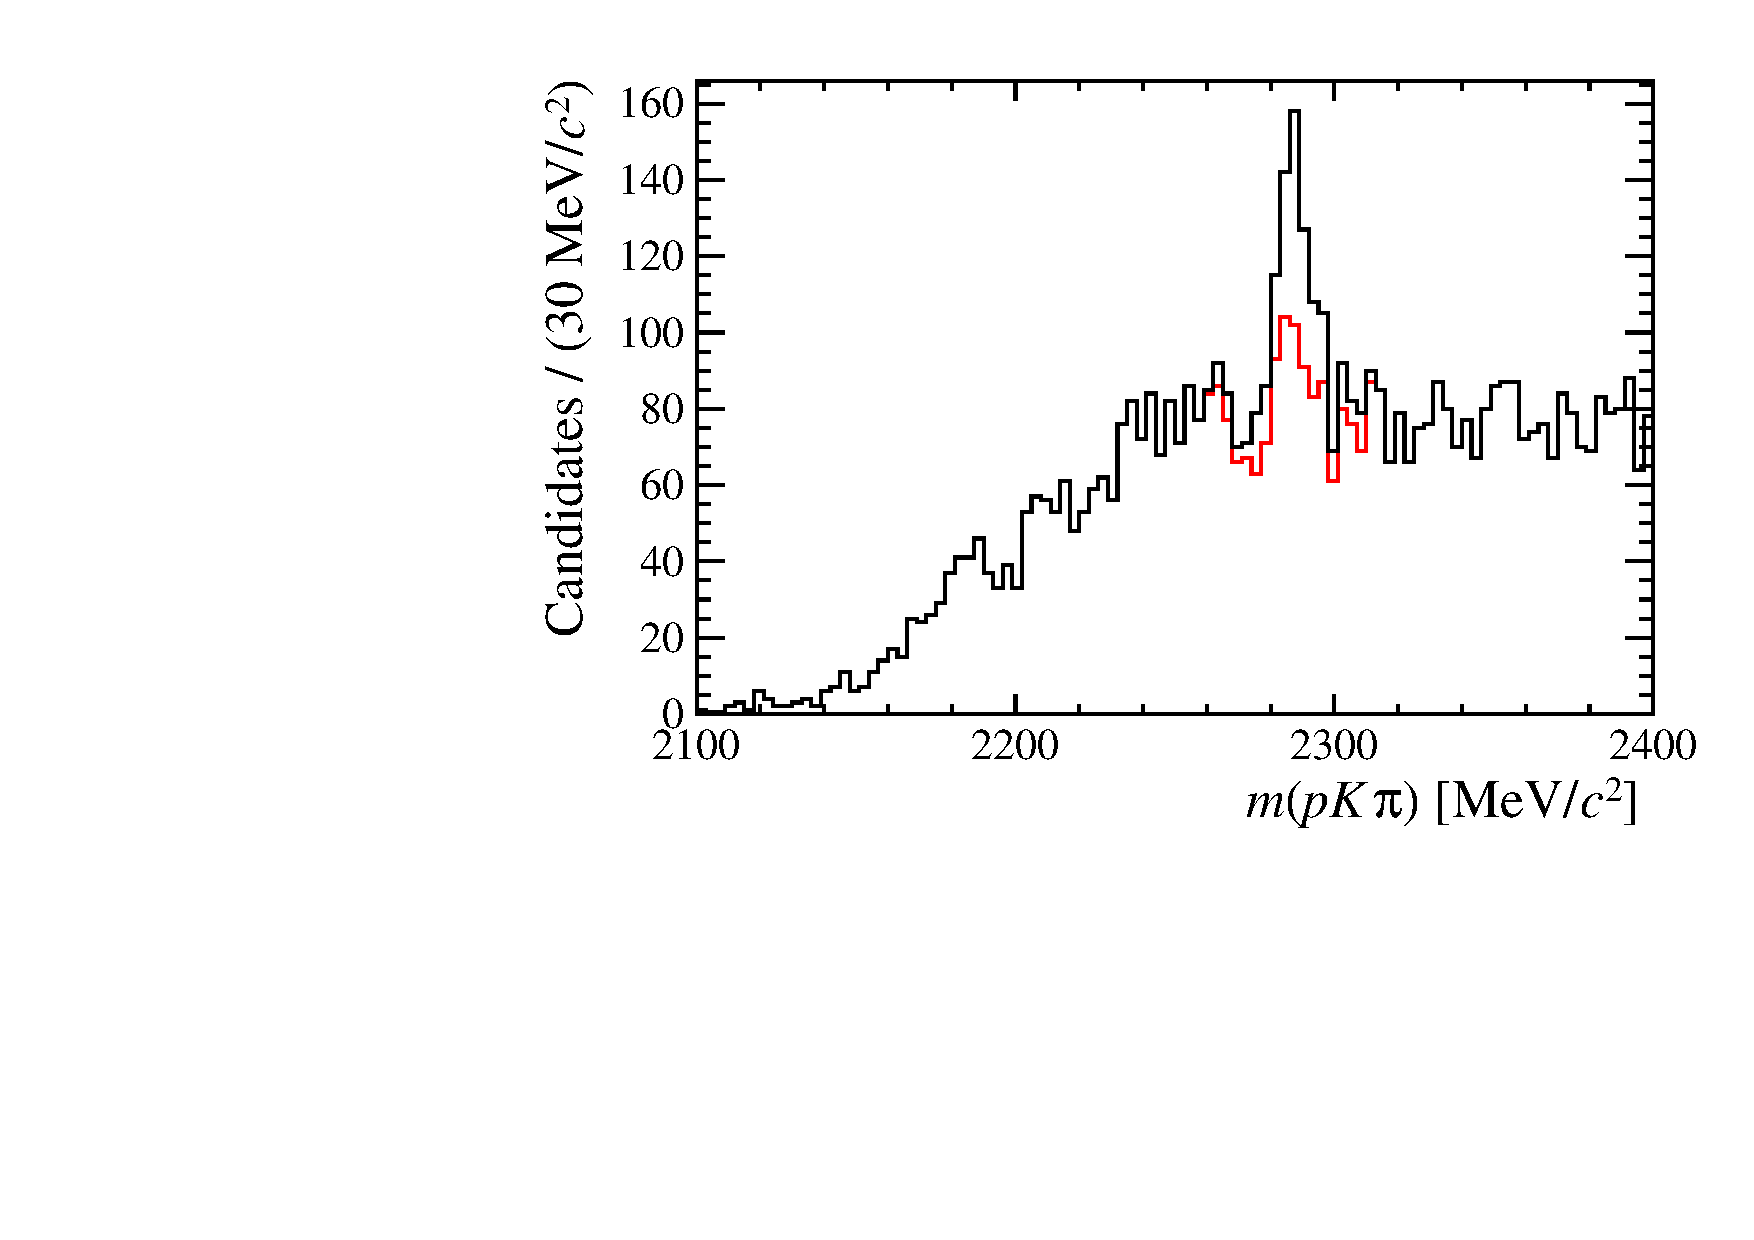
\includegraphics[width=1.0\textwidth]{figs/Selection/B2DsPhi_Ds2KKPi_Lc_Veto_WithBDT.pdf}
%         \caption{Signal with MVA cut}
%     \end{subfigure}\\
%     \caption{Invariant mass distributions of \decay{\Dsp}{\Kp\Km\pip} samples reconstructed as \decay{\Lc}{\Pp\Km\pip} for the signal and normalisation samples. The samples are shown with (red) and without (black) the veto described in Sec.~\ref{sec:pidvetos}. The distributions are shown before (top) and after (bottom) the MVA requirements have been applied.}
%     \label{fig:PIDVetos_Ds2KKPi_Lc_Veto}   
% \end{figure}
% %%%%%%%%%%%%%%%%%%%%%%%%%%%%%%%%%%%%%%%%%%%%%%%%%%%%%%%%%%

%%%%%%%%%%%%%%%%%%%%%%%%%%%%%%%%%%%%%%%%%%%%%%%%%%%%%%%%%%
\begin{figure}[!h]
    \centering
    \begin{subfigure}[t]{0.49\textwidth}
        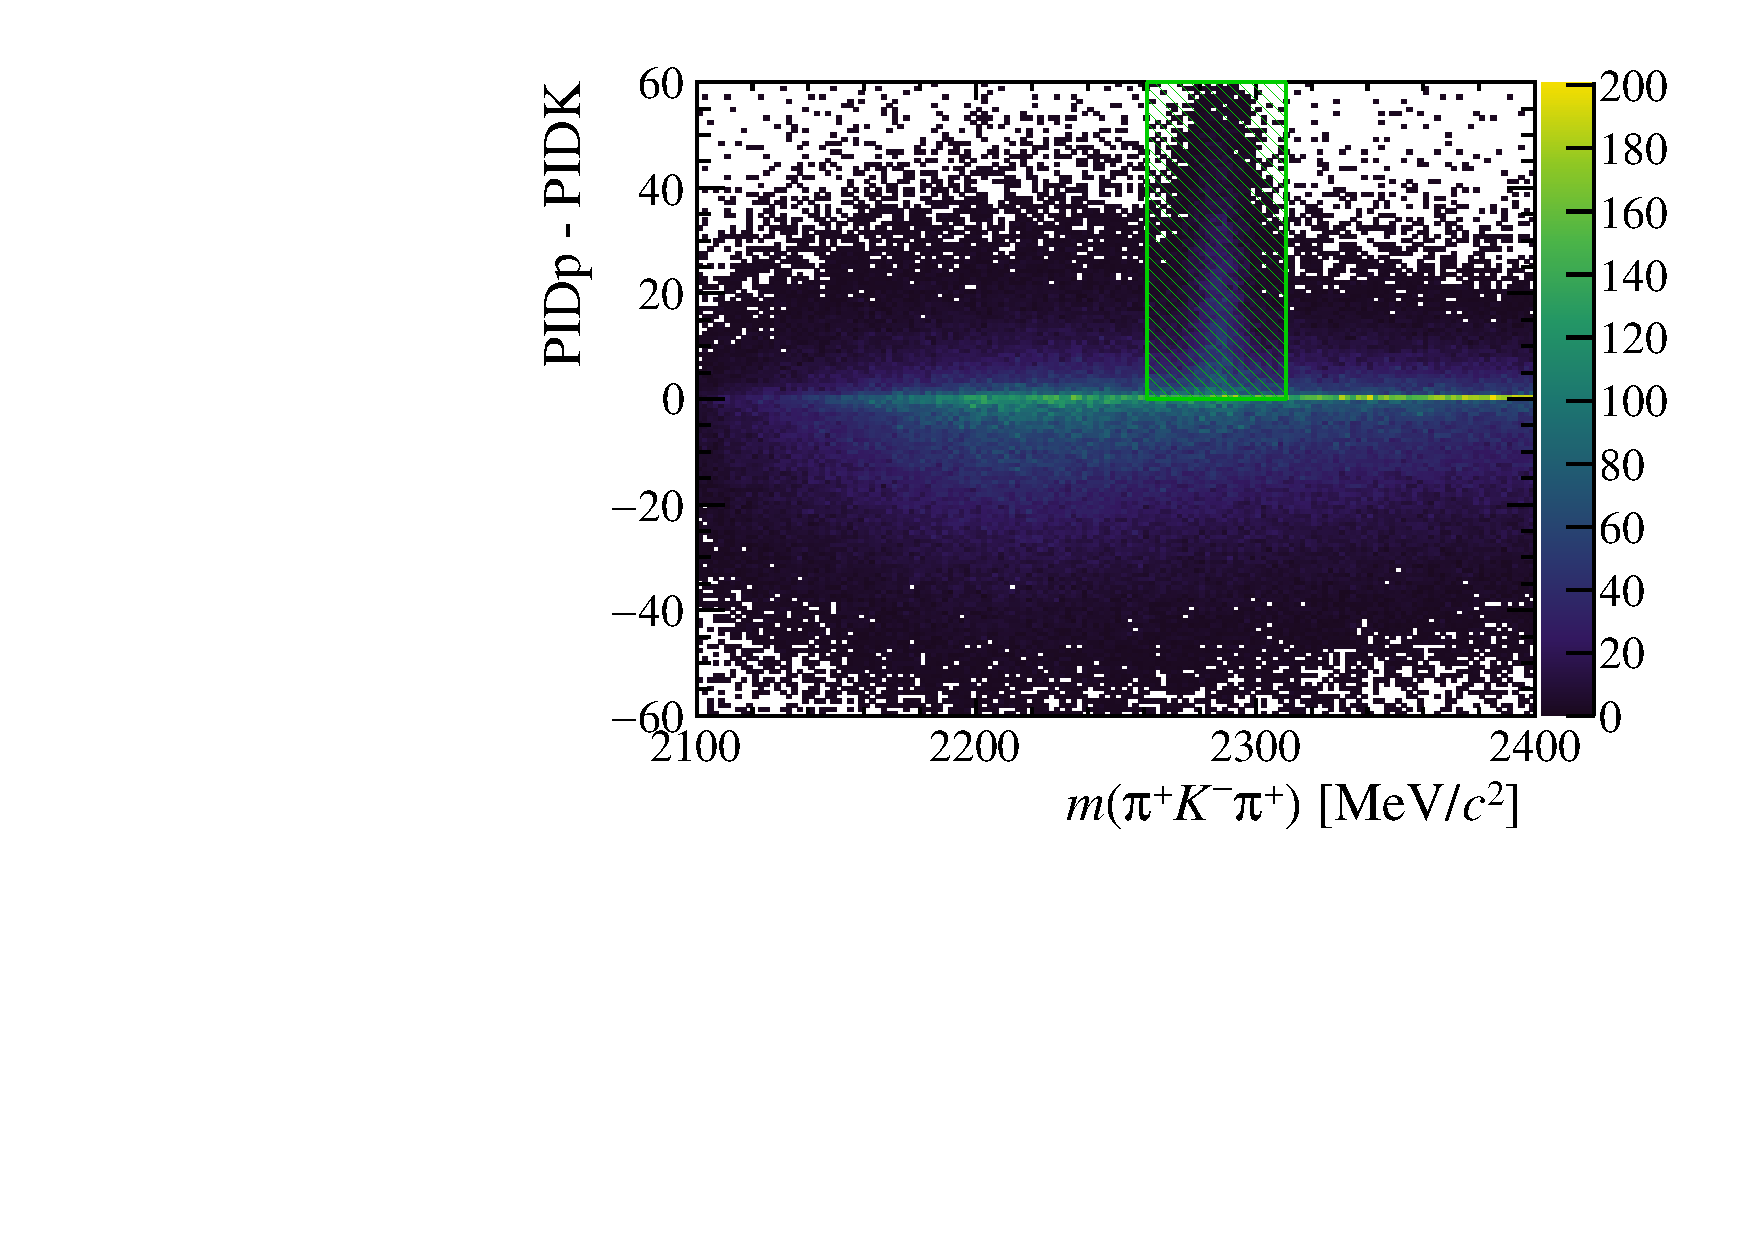
\includegraphics[width=1.0\textwidth]{figs/Selection/B2DsPhi_Ds2KKPi_2D_Lc_Veto_NoBDT.pdf}
        %\caption{Normalisation without MVA cut}
    \end{subfigure}%
    \begin{subfigure}[t]{0.49\textwidth}
        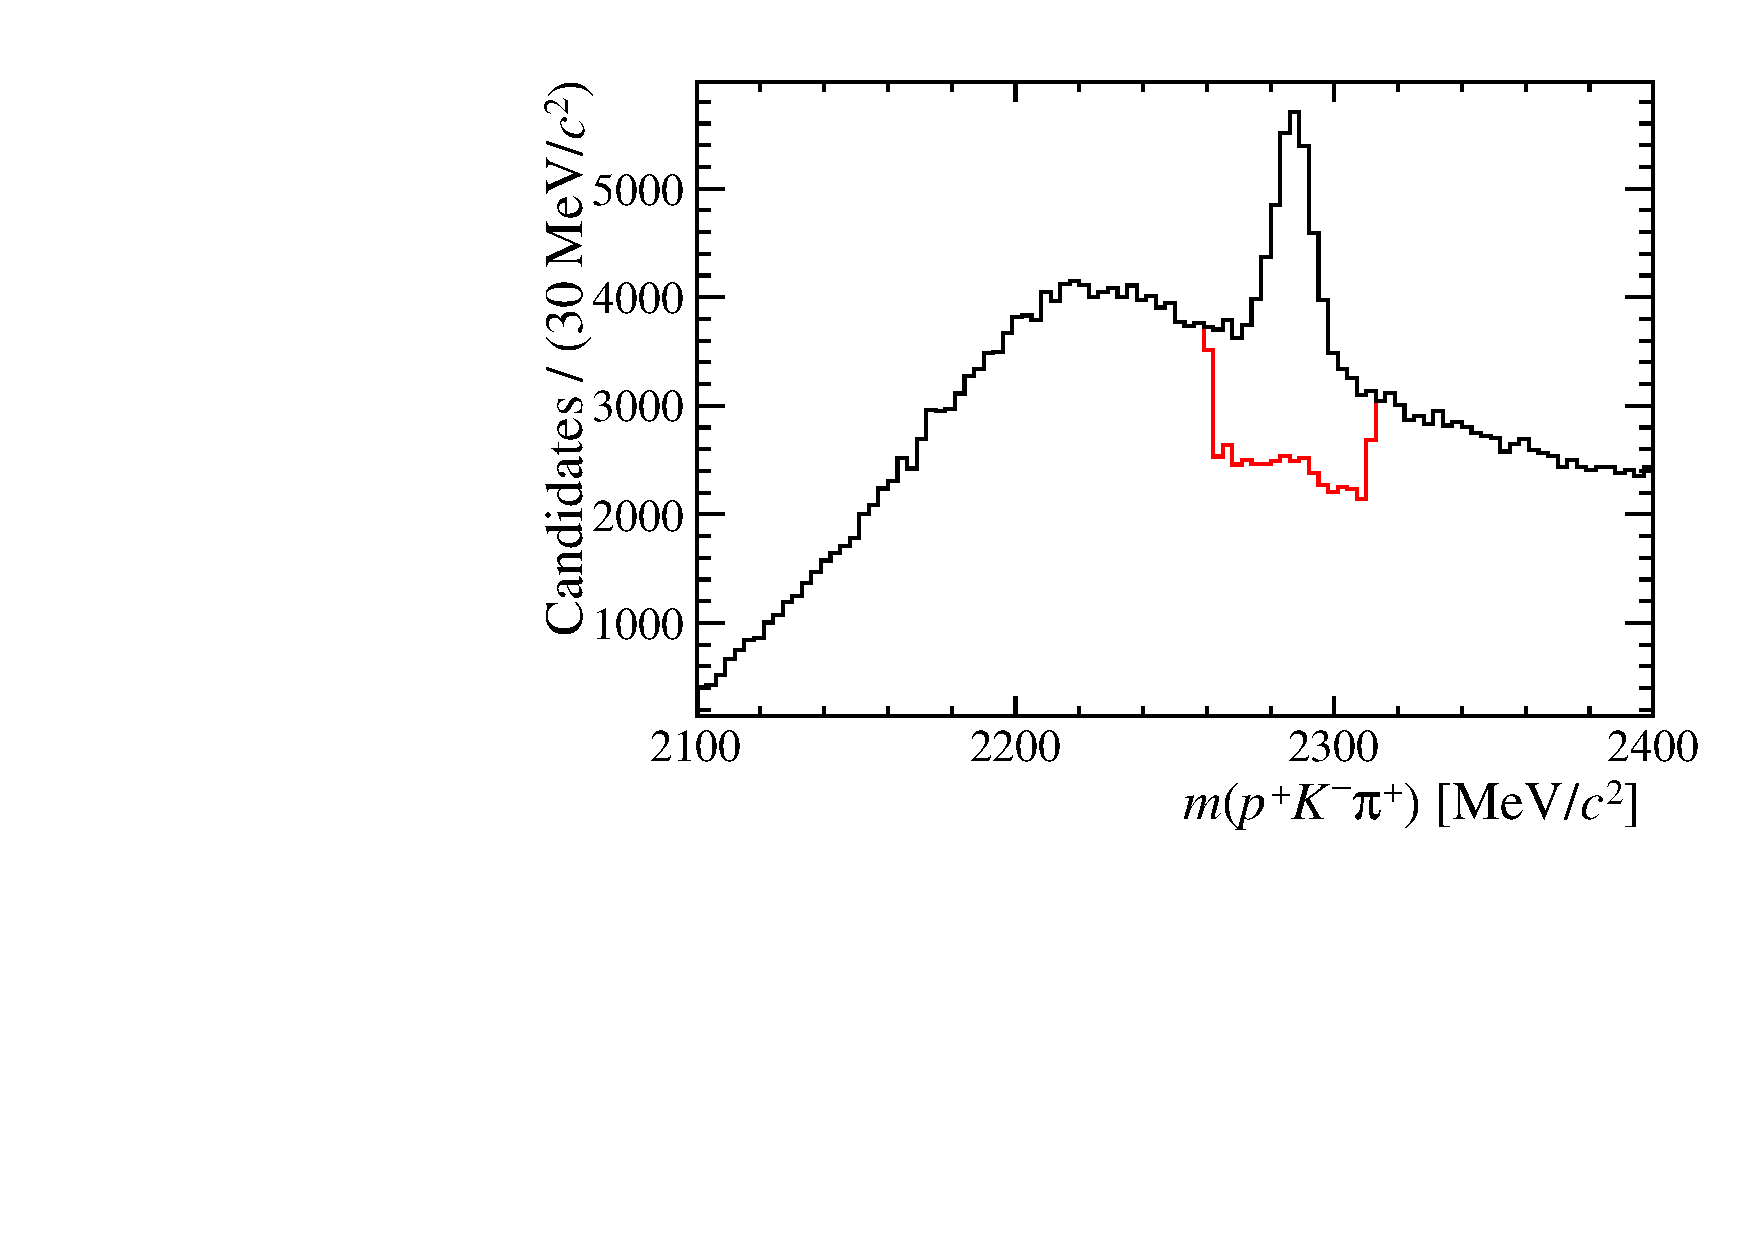
\includegraphics[width=1.0\textwidth]{figs/Selection/B2DsPhi_Ds2KKPi_Lc_Veto_NoBDT.pdf}
        %\caption{Signal without MVA cut}
    \end{subfigure}\\
    \caption{The invariant mass distributions of \decay{\Dsp}{\Kp\Km\pip} samples reconstructed as \decay{\Lc}{\Pp\Km\pip} plotted against the particle identification variables $\text{PIDp}-\text{PIDK}$ of the \Kp track (left). The green box represents the area removed by the veto. The misidentified invariant mass distribution (right) is plotted with (red) and without (black) the veto applied.}
    \label{fig:PIDVetos_Ds2KKPi_Lc_Veto}   
\end{figure}
%%%%%%%%%%%%%%%%%%%%%%%%%%%%%%%%%%%%%%%%%%%%%%%%%%%%%%%%%%



\subsection{Invariant mass vetoes}
\label{sec:kinematicvetos}

Sharp peaking structures are observed in invariant masses of subsets of the final state particles. These result from various signal or background processes in which incorrect tracks have been assigned to the the final state particles.   
These are removed with simple invariant mass cuts to remove combinatorial or partially reconstructed backgrounds that result from these incorrectly reconstructed decays. 
All combinations of the final state particles that create a neutral or singly-charged candidate are investigated.
Significant structures are observed for all three \Dsp decay modes in some combination as detailed in Appendix~\ref{sec:app_sel_vetoes}.


% For simplicity the final state particles for each mode are labelled with a number between 1--5 as described in Table~\ref{table:vetolabels}.

% \begin{table*}[!ht]
% \centering
% \begin{tabular}{ l c c c c c c }
% \hline
% Decay Mode & 1  & 2 & 3 & 4 & 5 \\
% \hline
% \decay{\Bp}{(\decay{\Dsp}{\Kp\Km\pip})\phiz}       & \Kp    & \Km    & \pip  & \Kp  & \Km \\
% \decay{\Bp}{(\decay{\Dsp}{\pip\pim\pip})\phiz}     & \pip   & \pim   & \pip  & \Kp  & \Km \\
% \decay{\Bp}{(\decay{\Dsp}{\Kp\pim\pip})\phiz}      & \Kp    & \pim   & \pip  & \Kp  & \Km \\
% \hline
% \decay{\Bp}{(\decay{\Dsp}{\Kp\Km\pip})\Kp\Km}      & \Kp    & \Km    & \pip  & \Kp  & \Km \\
% \hline
% \end{tabular}
% \caption{Particle labels used when studying invariant mass vetoes for \decay{\Bp}{\Dsp\phiz} and \decay{\Bp}{\Dsp\Kp\Km} candidates.}
% \label{table:vetolabels}

% \end{table*}

% All combinations of the final state particles that create a neutral or singly-charged candidate are investigated.
% Significant structures are observed for all three \Dsp decay modes in some combination. 

% The following vetos are applied to remove these incorrectly reconstructed decays.
% \begin{itemize}
% \item For the mode \decay{\Bp}{(\decay{\Dsp}{\Kp\Km\pip})\phiz}
% \begin{itemize}
% \item $|m(\text{1245})- m(\Bs)| > 50\mevcc$
% \item $|m(\text{345})- m(\Dsp)| > 25\mevcc$ and $|m(\text{345})- m(\Dp)| > 25\mevcc$
% \end{itemize}

% \item For the mode \decay{\Bp}{(\decay{\Dsp}{\pip\pim\pip})\phiz}
% \begin{itemize}
% \item $|m(\text{145})- m(\Dsp)| > 25\mevcc$ and $|m(\text{145})- m(\Dp)| > 25\mevcc$
% \item $|m(\text{245})- m(\Dsp)| > 25\mevcc$ and $|m(\text{245})- m(\Dp)| > 25\mevcc$
% \item $|m(\text{345})- m(\Dsp)| > 25\mevcc$ and $|m(\text{345})- m(\Dp)| > 25\mevcc$
% \end{itemize}
% \item For the mode \decay{\Bp}{(\decay{\Dsp}{\Kp\pim\pip})\phiz}
% \begin{itemize}
% \item $|m(\text{245})- m(\Dsp)| > 25\mevcc$ and $|m(\text{245})- m(\Dp)| > 25\mevcc$
% \item $|m(\text{345})- m(\Dsp)| > 25\mevcc$ and $|m(\text{345})- m(\Dp)| > 25\mevcc$
% \end{itemize}
% \end{itemize}

% %%%%%%%%%%%%%%%%%%%%%%%%%%%%%%%%%%%%%%%%%%%%%%%%%%%%%%%%%%
% \begin{figure}[!h]
%    \centering
%    \begin{subfigure}[t]{1.0\textwidth}
%       \centering
%       \begin{subfigure}[t]{0.32\textwidth}
%          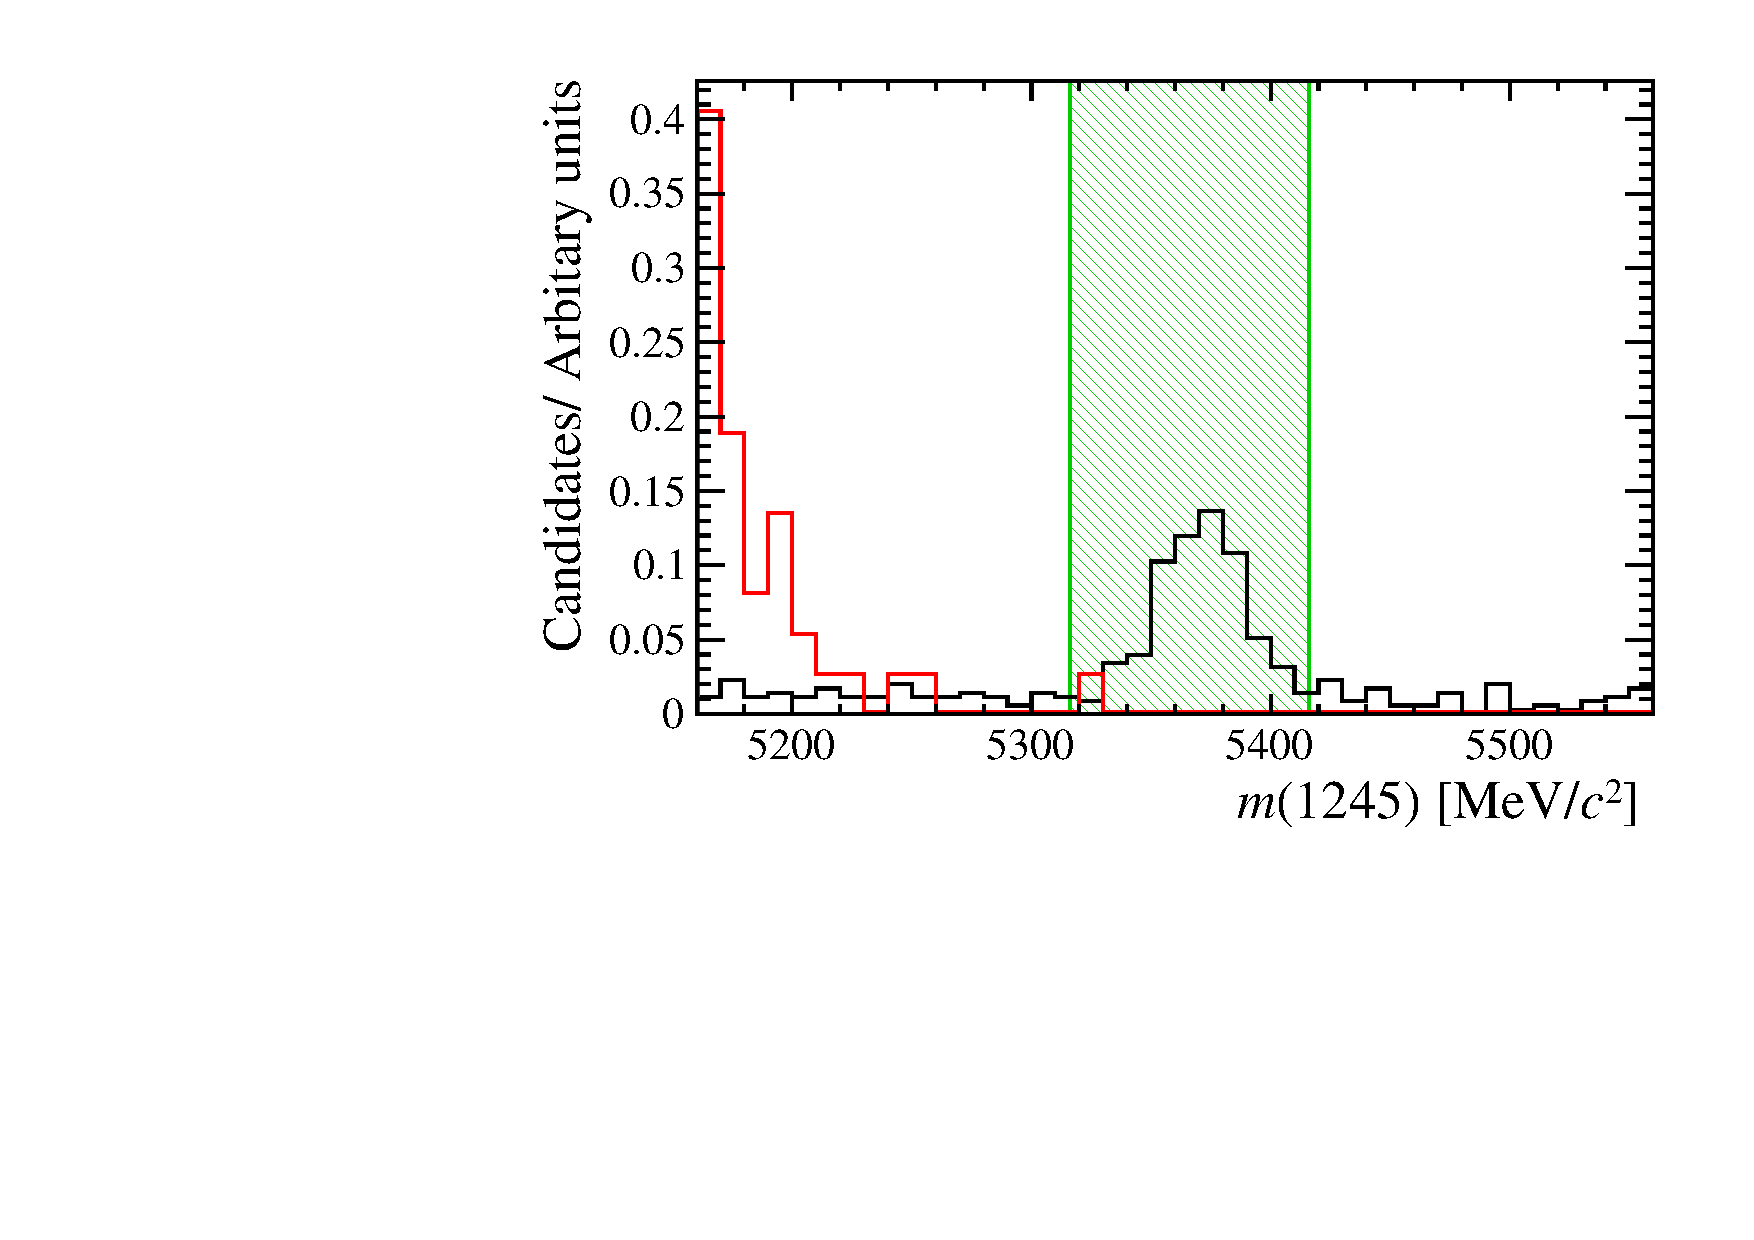
\includegraphics[width=1.0\textwidth]{figs/Selection/Veto_Comparison_B2DsPhi_Ds2KKPi_m1245.pdf}
%       \end{subfigure}
%       \begin{subfigure}[t]{0.32\textwidth}
%          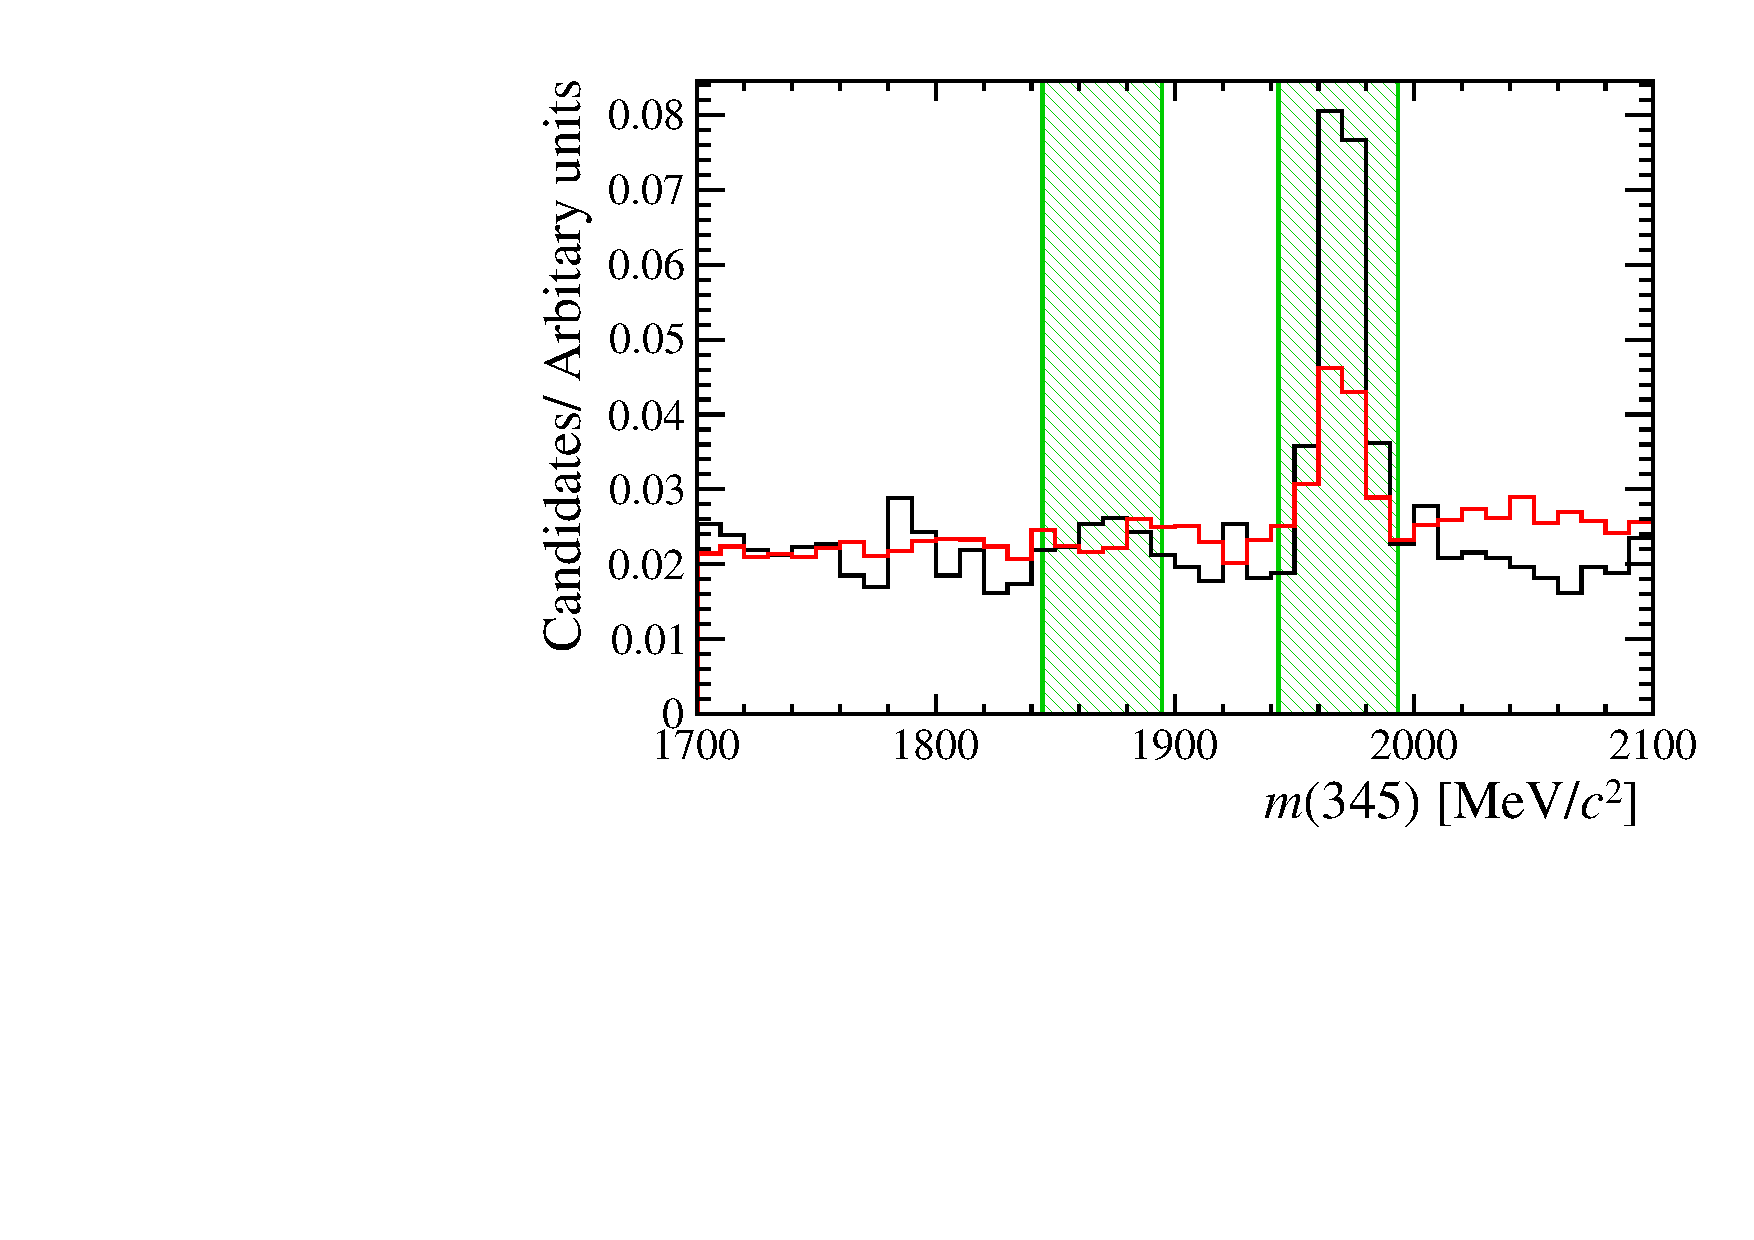
\includegraphics[width=1.0\textwidth]{figs/Selection/Veto_Comparison_B2DsPhi_Ds2KKPi_m345.pdf}
%       \end{subfigure}
%       \caption{\decay{\Bp}{(\decay{\Dsp}{\Kp\Km\pip})\phiz}}
%    \end{subfigure}
%    \begin{subfigure}[t]{1.0\textwidth}
%       \centering
%       \begin{subfigure}[t]{0.32\textwidth}
%          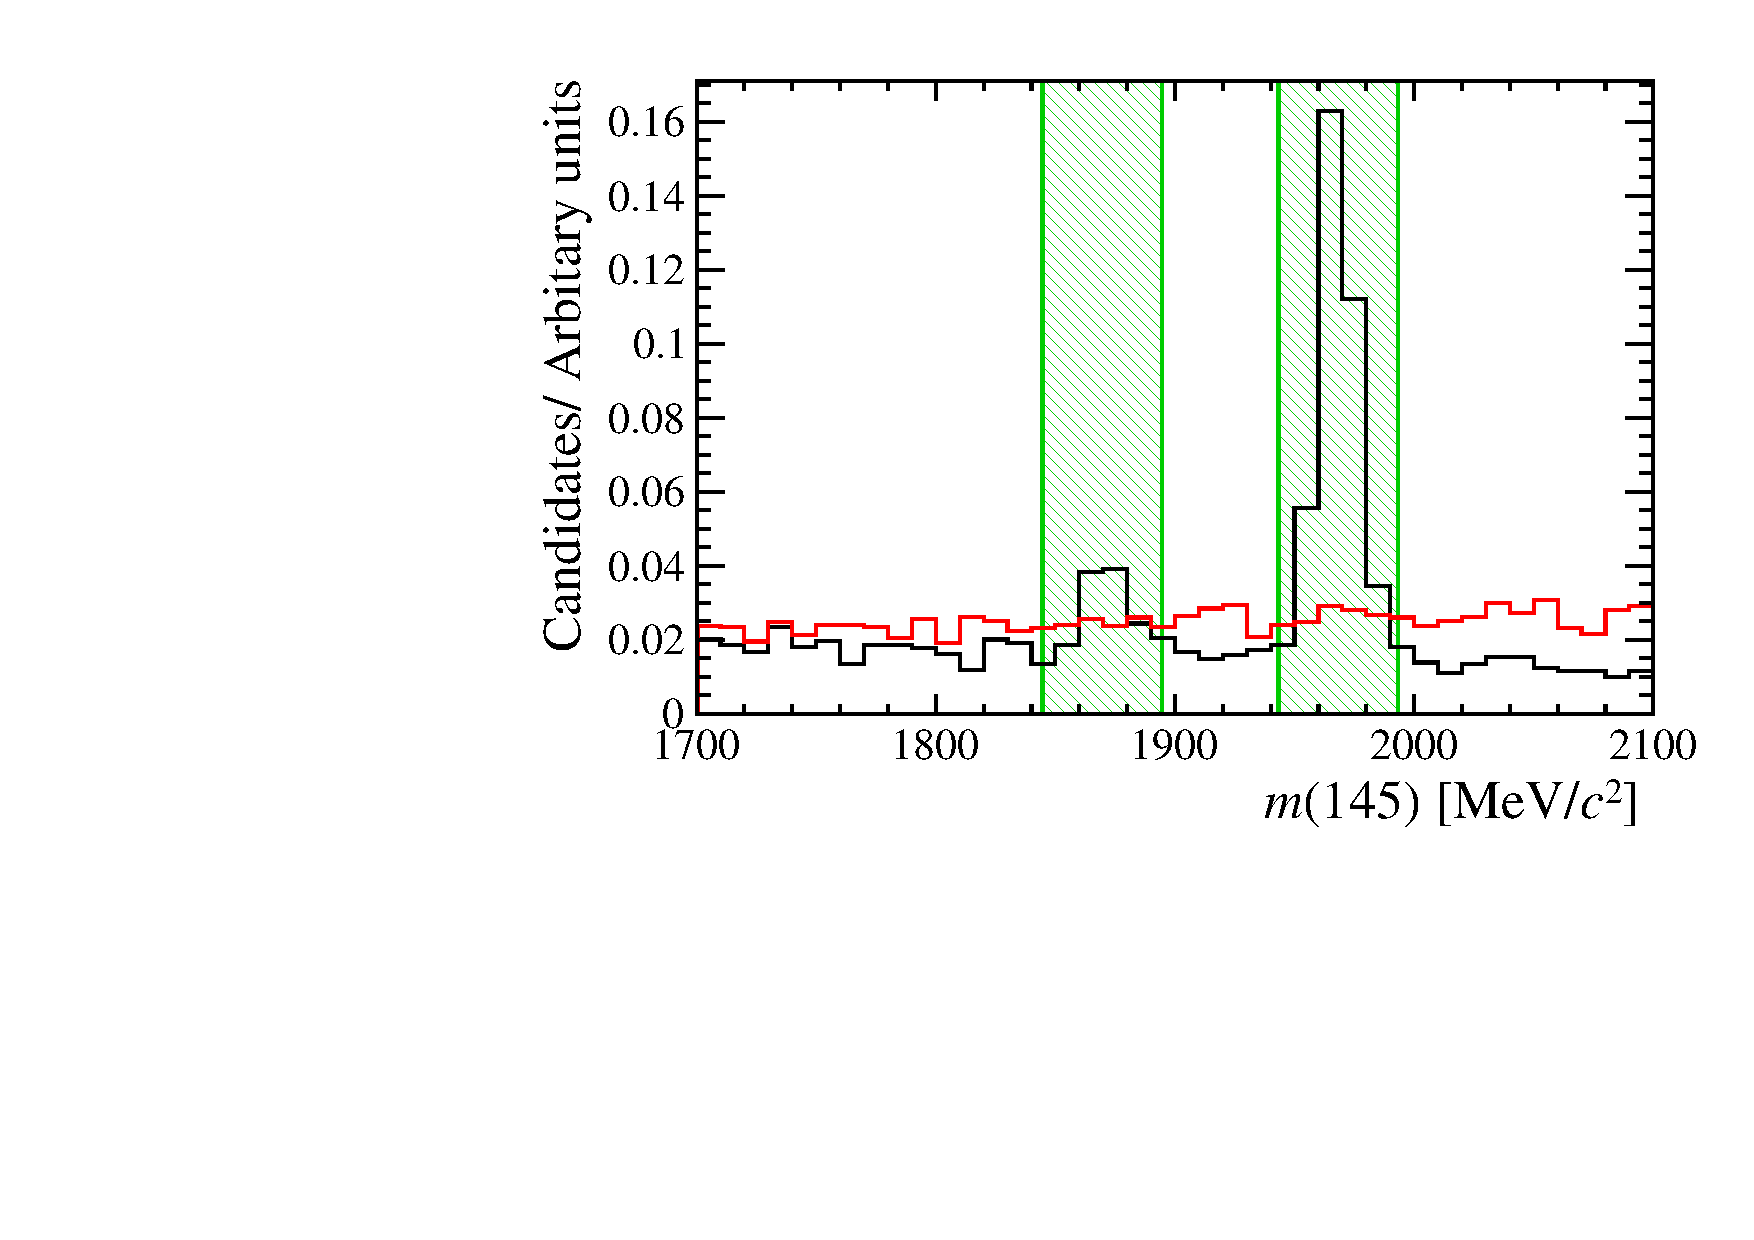
\includegraphics[width=1.0\textwidth]{figs/Selection/Veto_Comparison_B2DsPhi_Ds2PiPiPi_m145.pdf}
%       \end{subfigure}
%       \begin{subfigure}[t]{0.32\textwidth}
%          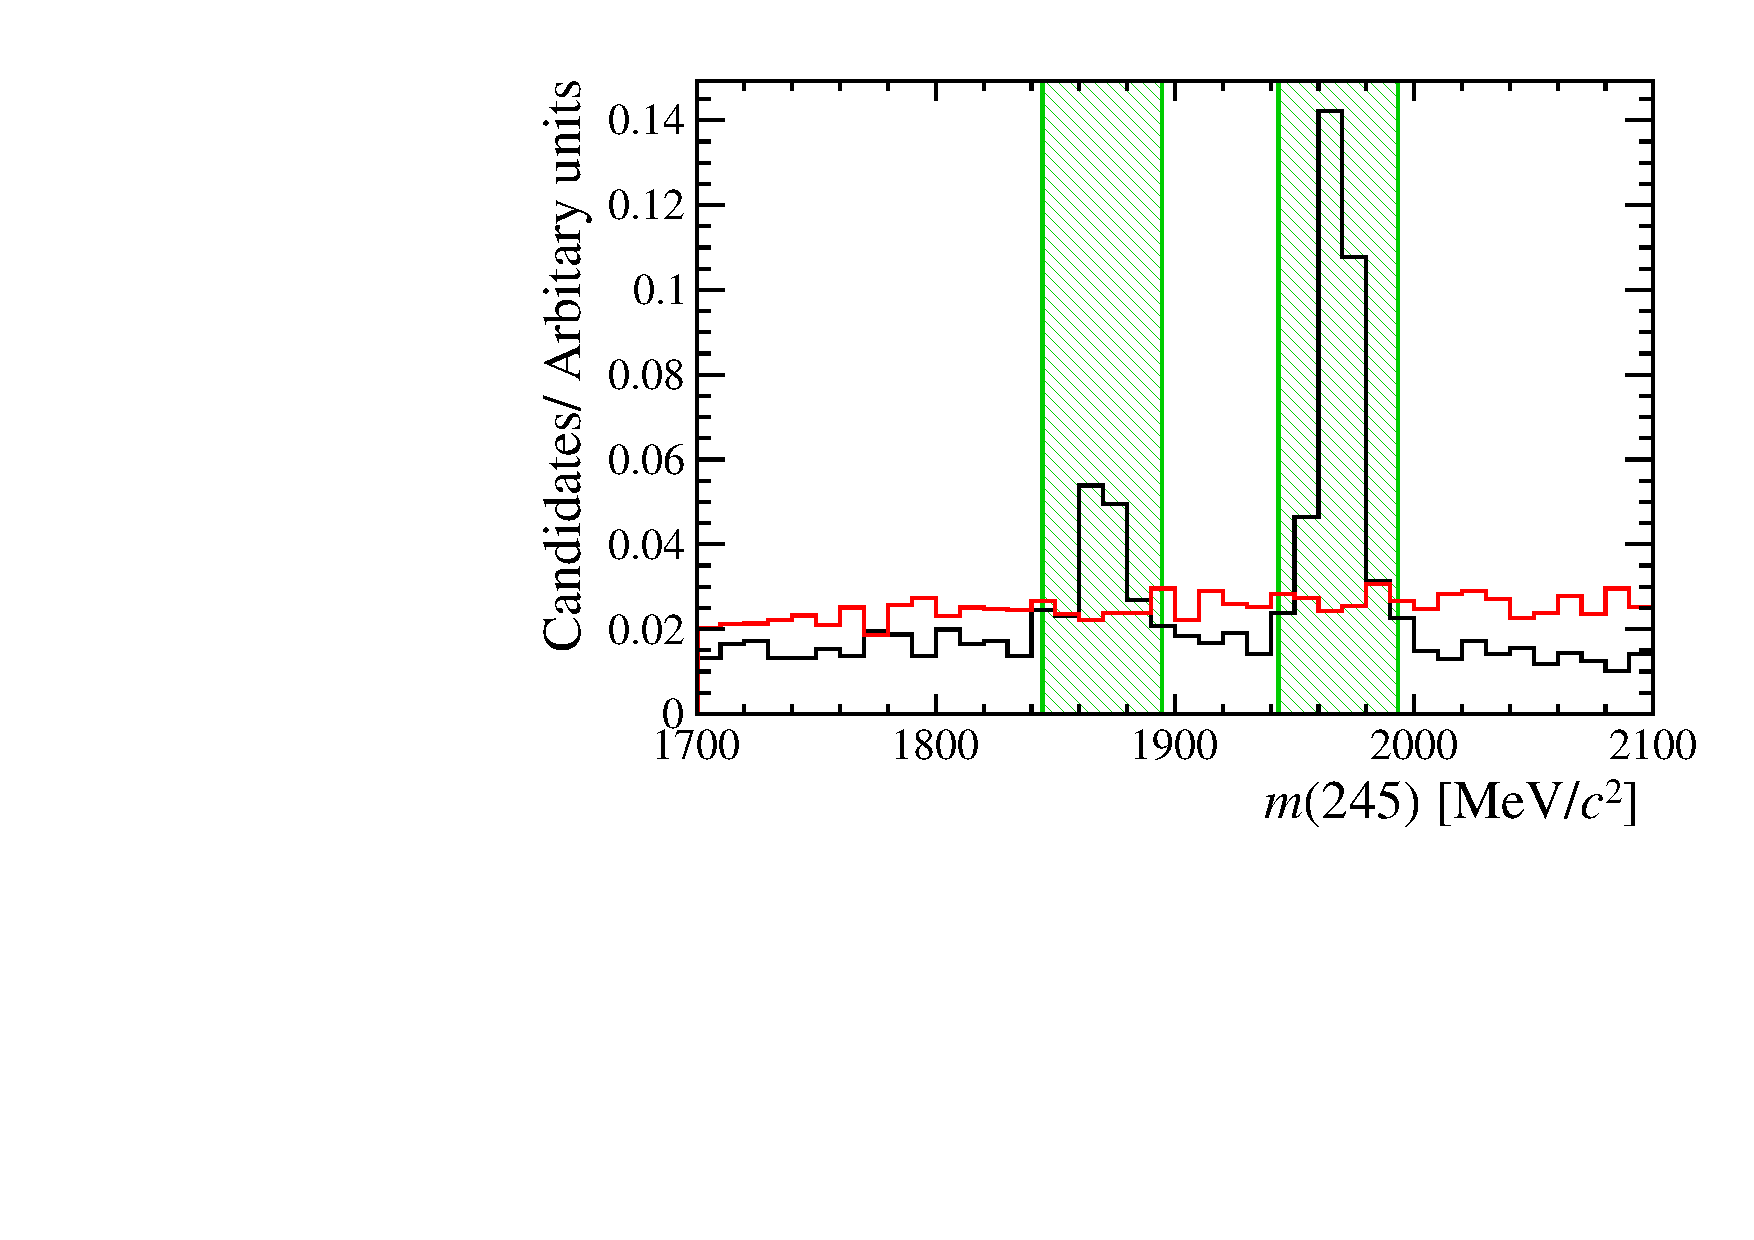
\includegraphics[width=1.0\textwidth]{figs/Selection/Veto_Comparison_B2DsPhi_Ds2PiPiPi_m245.pdf}
%       \end{subfigure}
%       \begin{subfigure}[t]{0.32\textwidth}
%          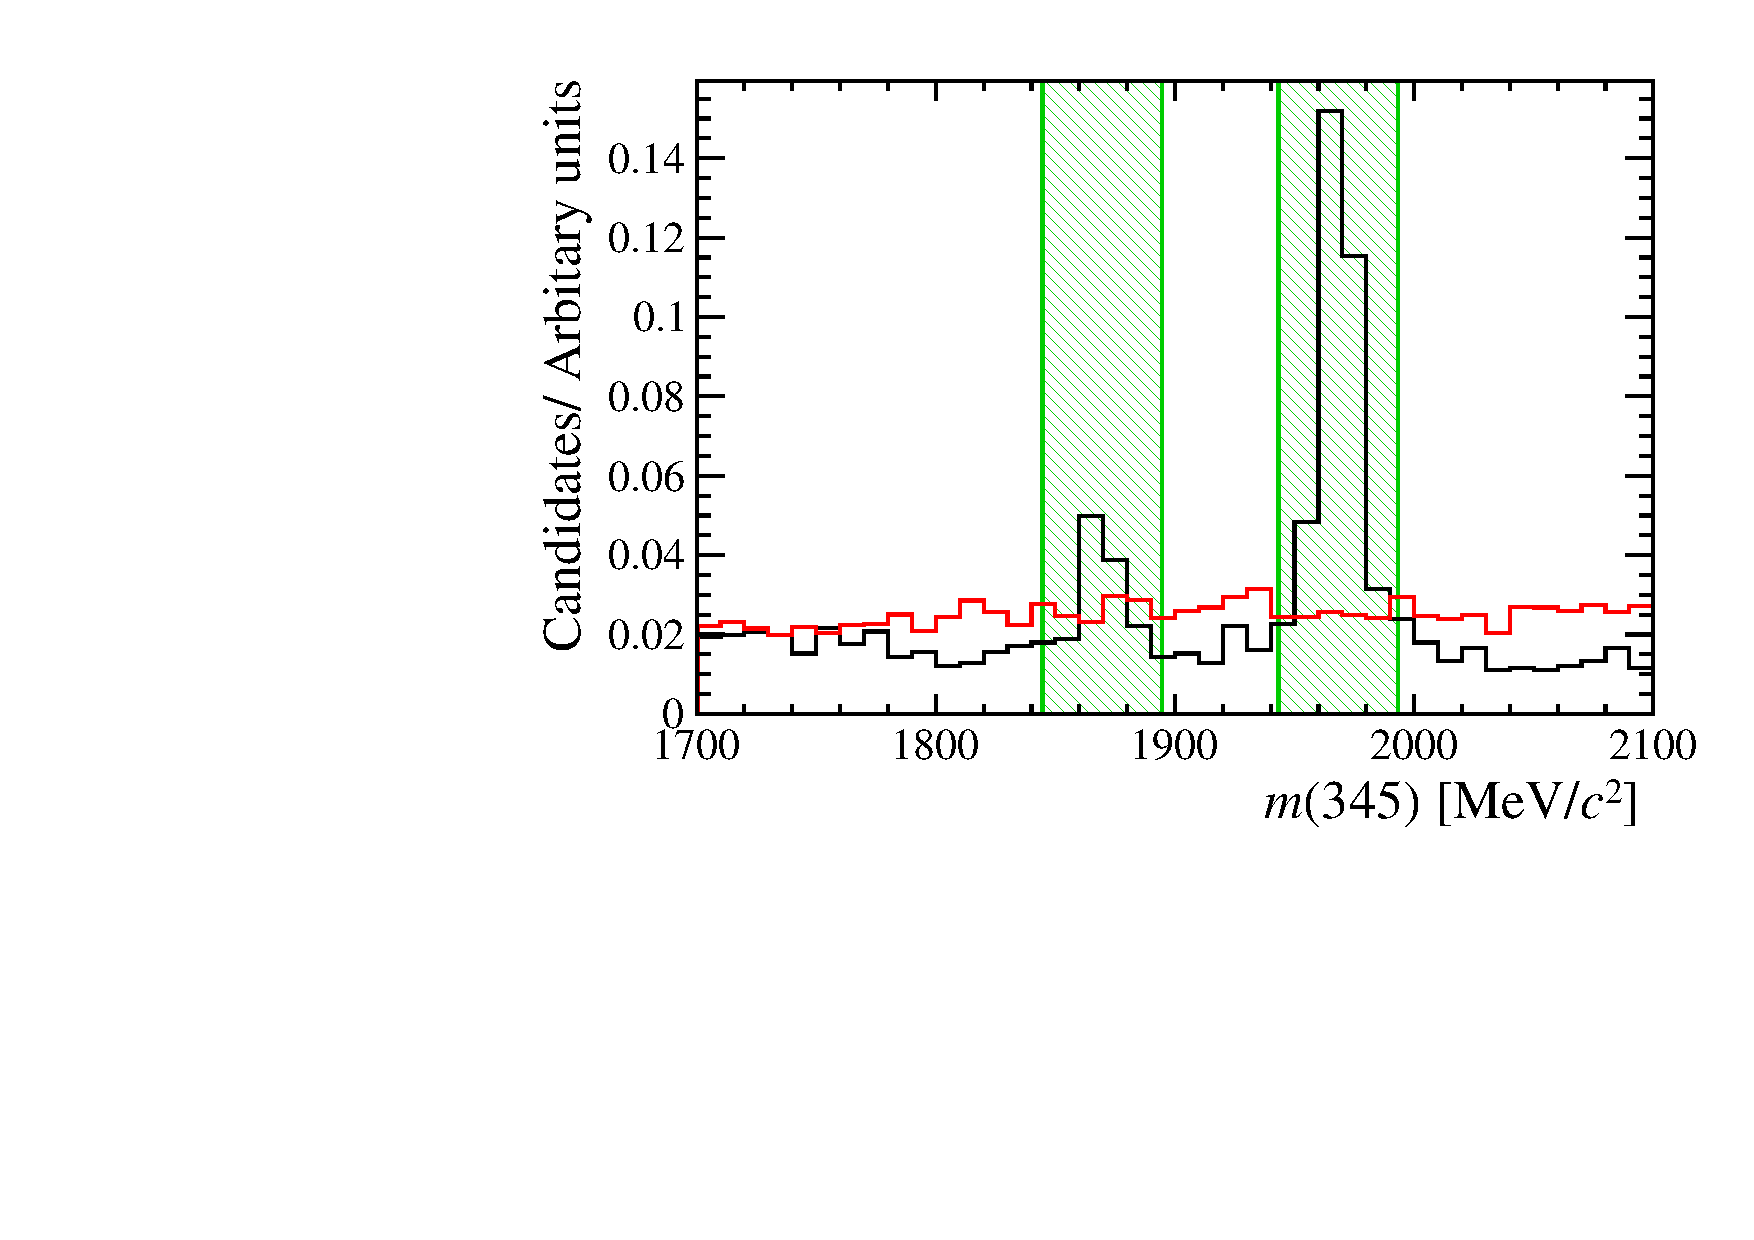
\includegraphics[width=1.0\textwidth]{figs/Selection/Veto_Comparison_B2DsPhi_Ds2PiPiPi_m345.pdf}
%       \end{subfigure}
%       \caption{\decay{\Bp}{(\decay{\Dsp}{\pip\pim\pip})\phiz}}
%    \end{subfigure}
%    \begin{subfigure}[t]{1.0\textwidth}
%       \centering
%       \begin{subfigure}[t]{0.32\textwidth}
%          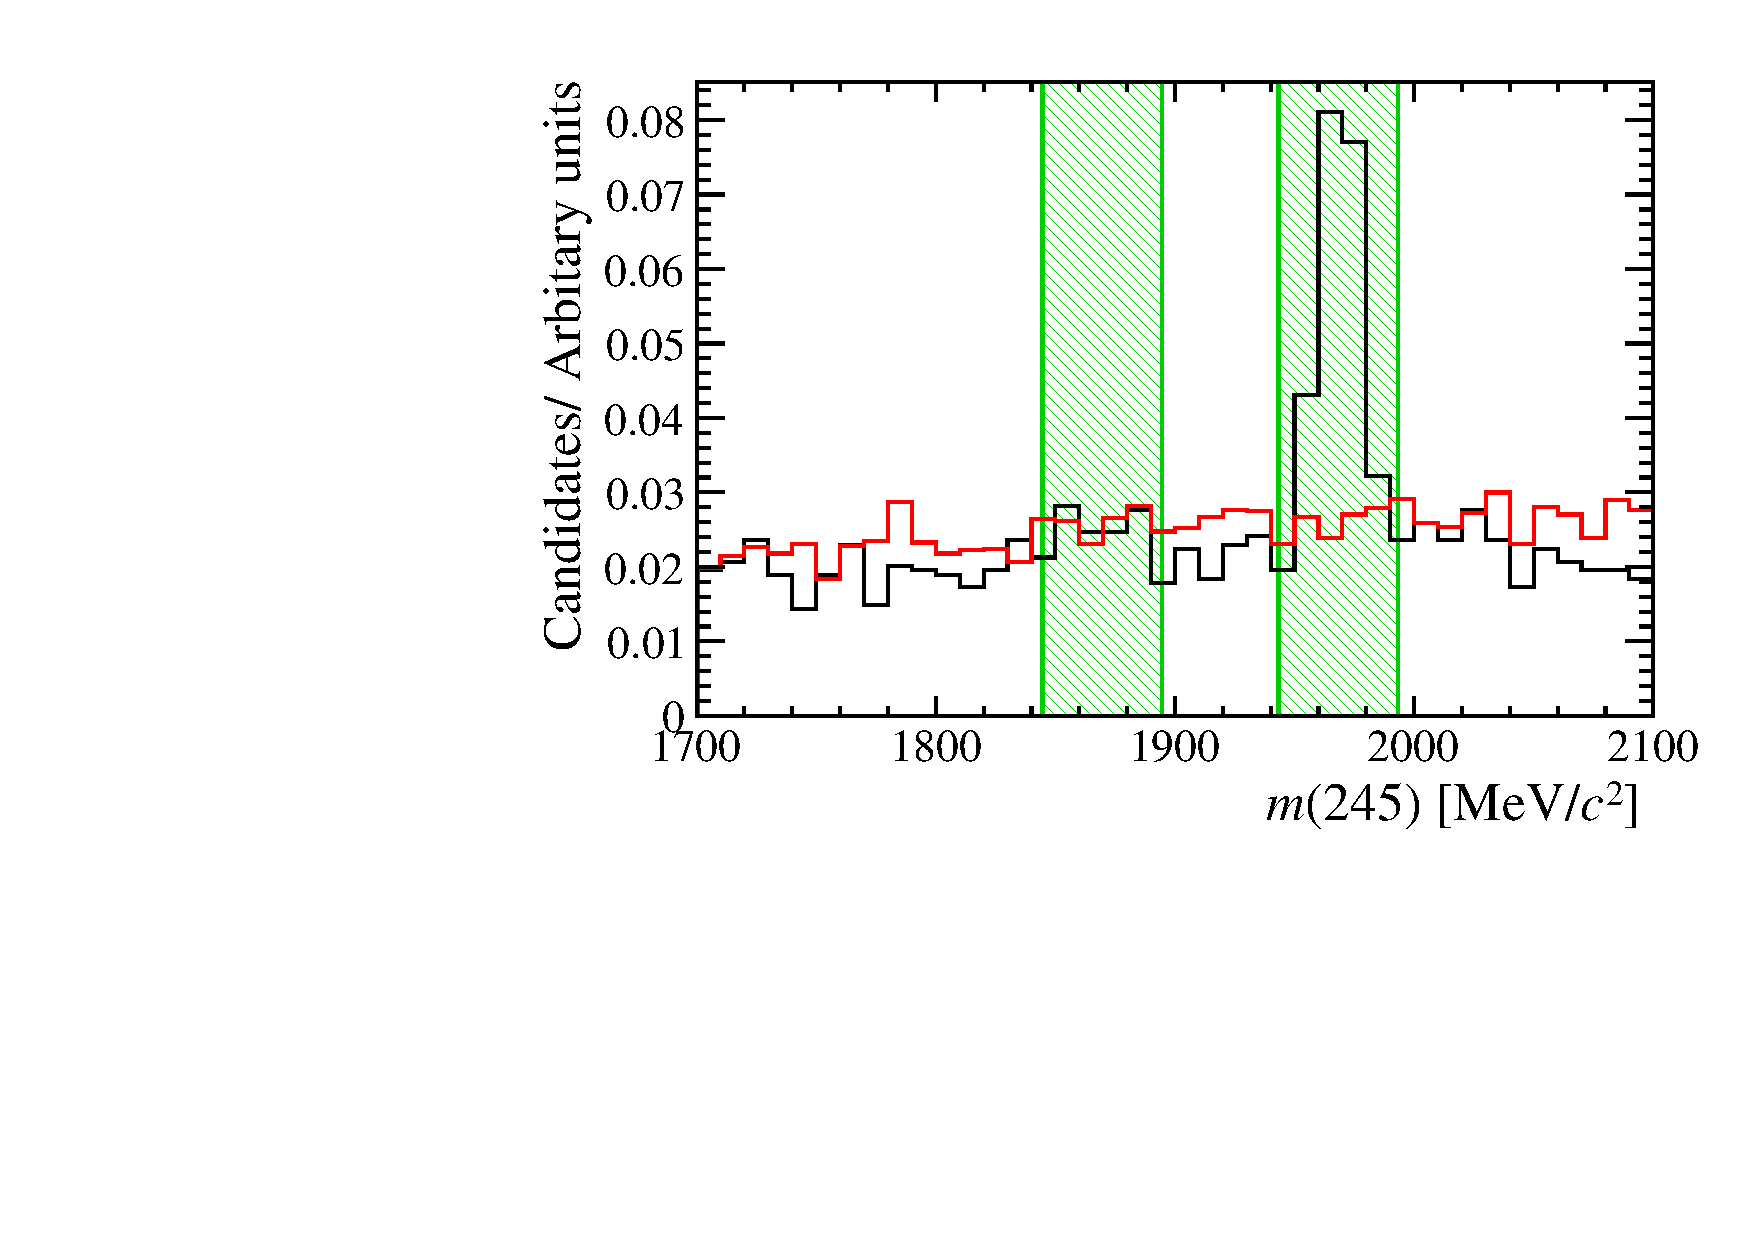
\includegraphics[width=1.0\textwidth]{figs/Selection/Veto_Comparison_B2DsPhi_Ds2KPiPi_m245.pdf}
%       \end{subfigure}
%       \begin{subfigure}[t]{0.32\textwidth}
%          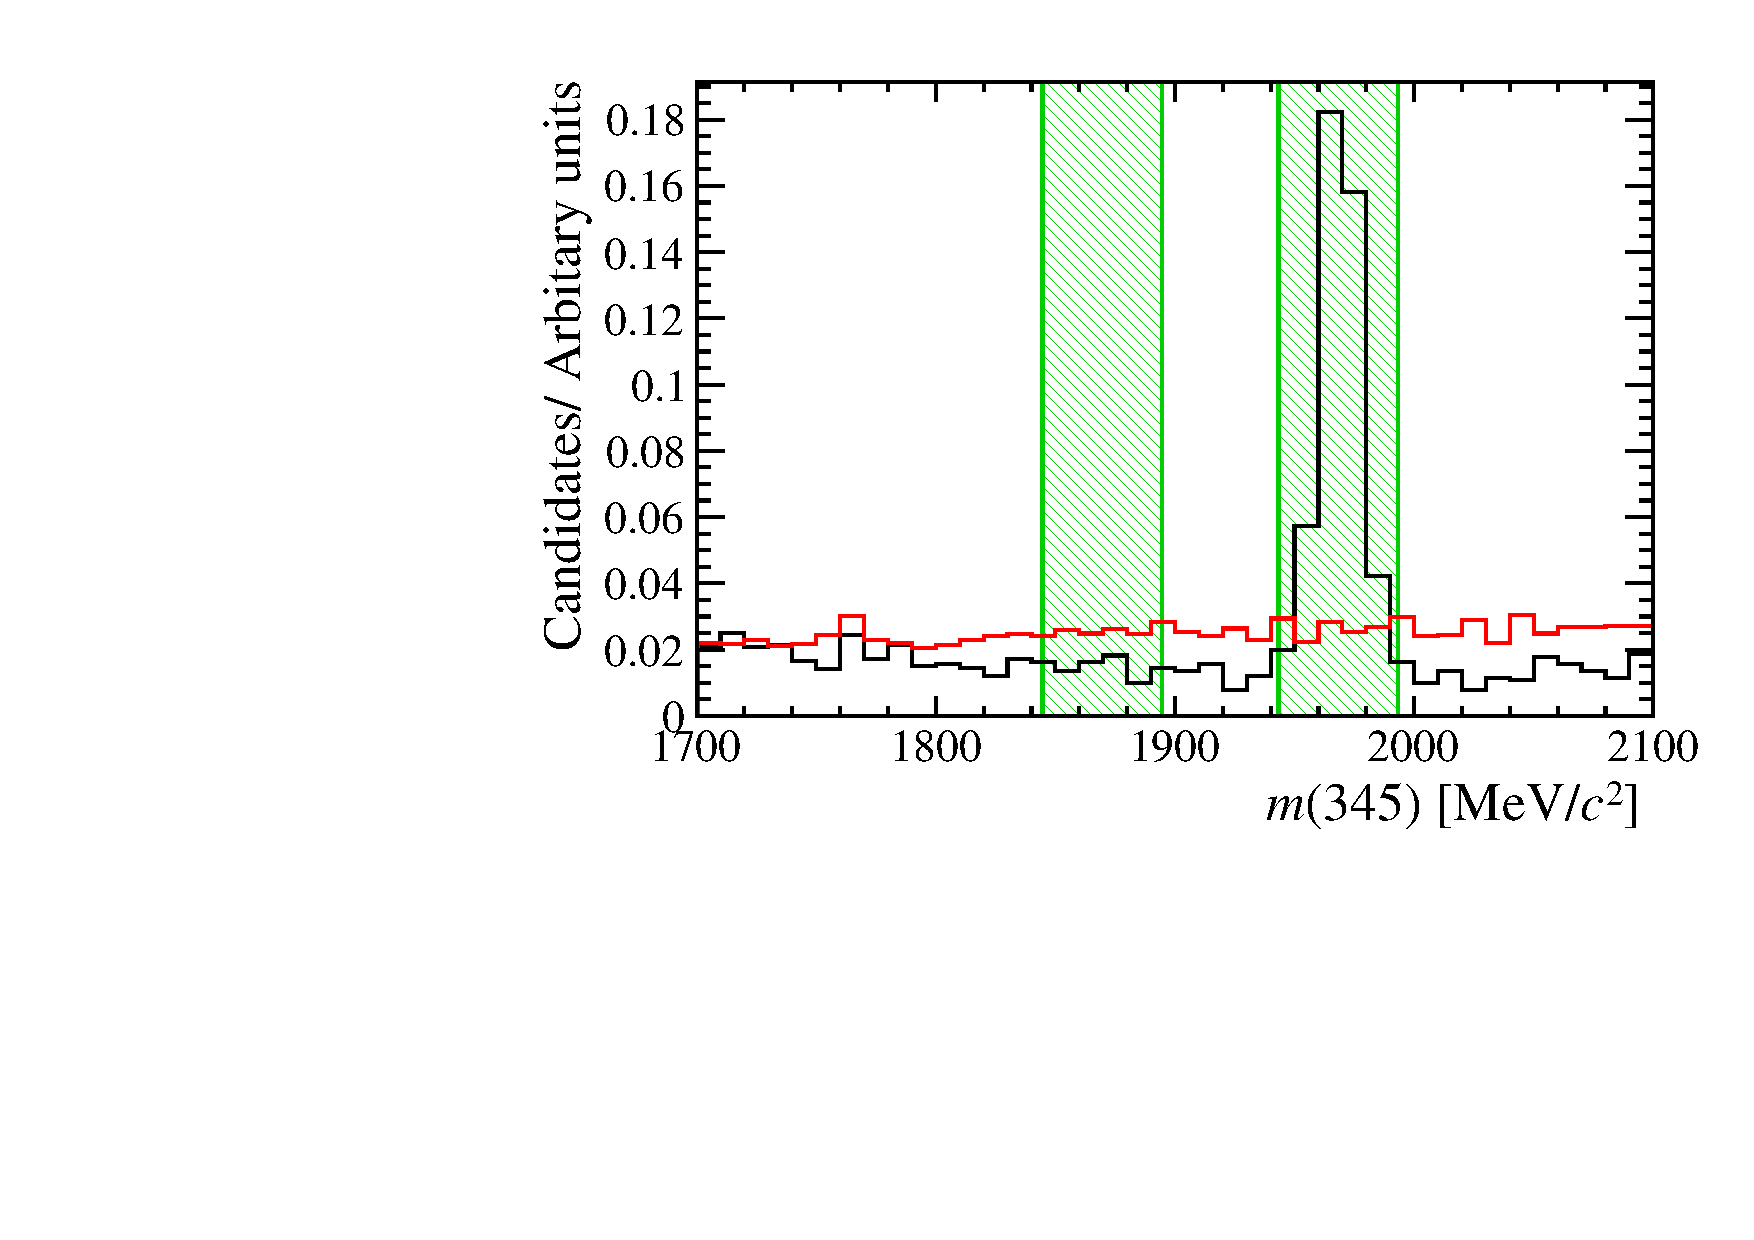
\includegraphics[width=1.0\textwidth]{figs/Selection/Veto_Comparison_B2DsPhi_Ds2KPiPi_m345.pdf}
%       \end{subfigure}
%       \caption{\decay{\Bp}{(\decay{\Dsp}{\Kp\pim\pip})\phiz}}
%    \end{subfigure}

%    \caption{Invariant mass distributions for subsets of decay products in data (black) and simulation (red). The green region show the regions removed by the vetoes listed in Sec~\ref{sec:kinematicvetos}.}
%    \label{fig:invariantmassvetoes}   
% \end{figure}
% %%%%%%%%%%%%%%%%%%%%%%%%%%%%%%%%%%%%%%%%%%%%%%%%%%%%%%%%%%


% In the search for \decay{\Bp}{\Dsp\Kp\Km} decays the increased size of the $m(\Kp\Km)$ phase-space means more of the combinations of final state particles are susceptible to sharp peaking structure from incorrectly reconstructed backgrounds. Those spectra found to have significant peaking structures are additionally vetoed, as shown in Fig.~\ref{fig:invariantmassvetoes_DsKK}.

% \begin{itemize}
% \item Vetoes for the mode \decay{\Bp}{(\decay{\Dsp}{\Kp\Km\pip})\Kp\Km}:
% \begin{itemize}
% \item $|m(\text{1245})- m(\Bs)| > 50\mevcc$
% \item $|m(\text{345})- m(\Dsp)| > 25\mevcc$ and $|m(\text{345})- m(\Dp)| > 25\mevcc$
% \item $|m(\text{135})- m(\Dsp)| > 25\mevcc$
% \item $|m(\text{234})- m(\Dsp)| > 25\mevcc$
% \end{itemize}
% \end{itemize}

% %%%%%%%%%%%%%%%%%%%%%%%%%%%%%%%%%%%%%%%%%%%%%%%%%%%%%%%%%%
% \begin{figure}[!h]
%    \centering
%    \begin{subfigure}[t]{1.0\textwidth}
%       \centering
%       \begin{subfigure}[t]{0.32\textwidth}
%          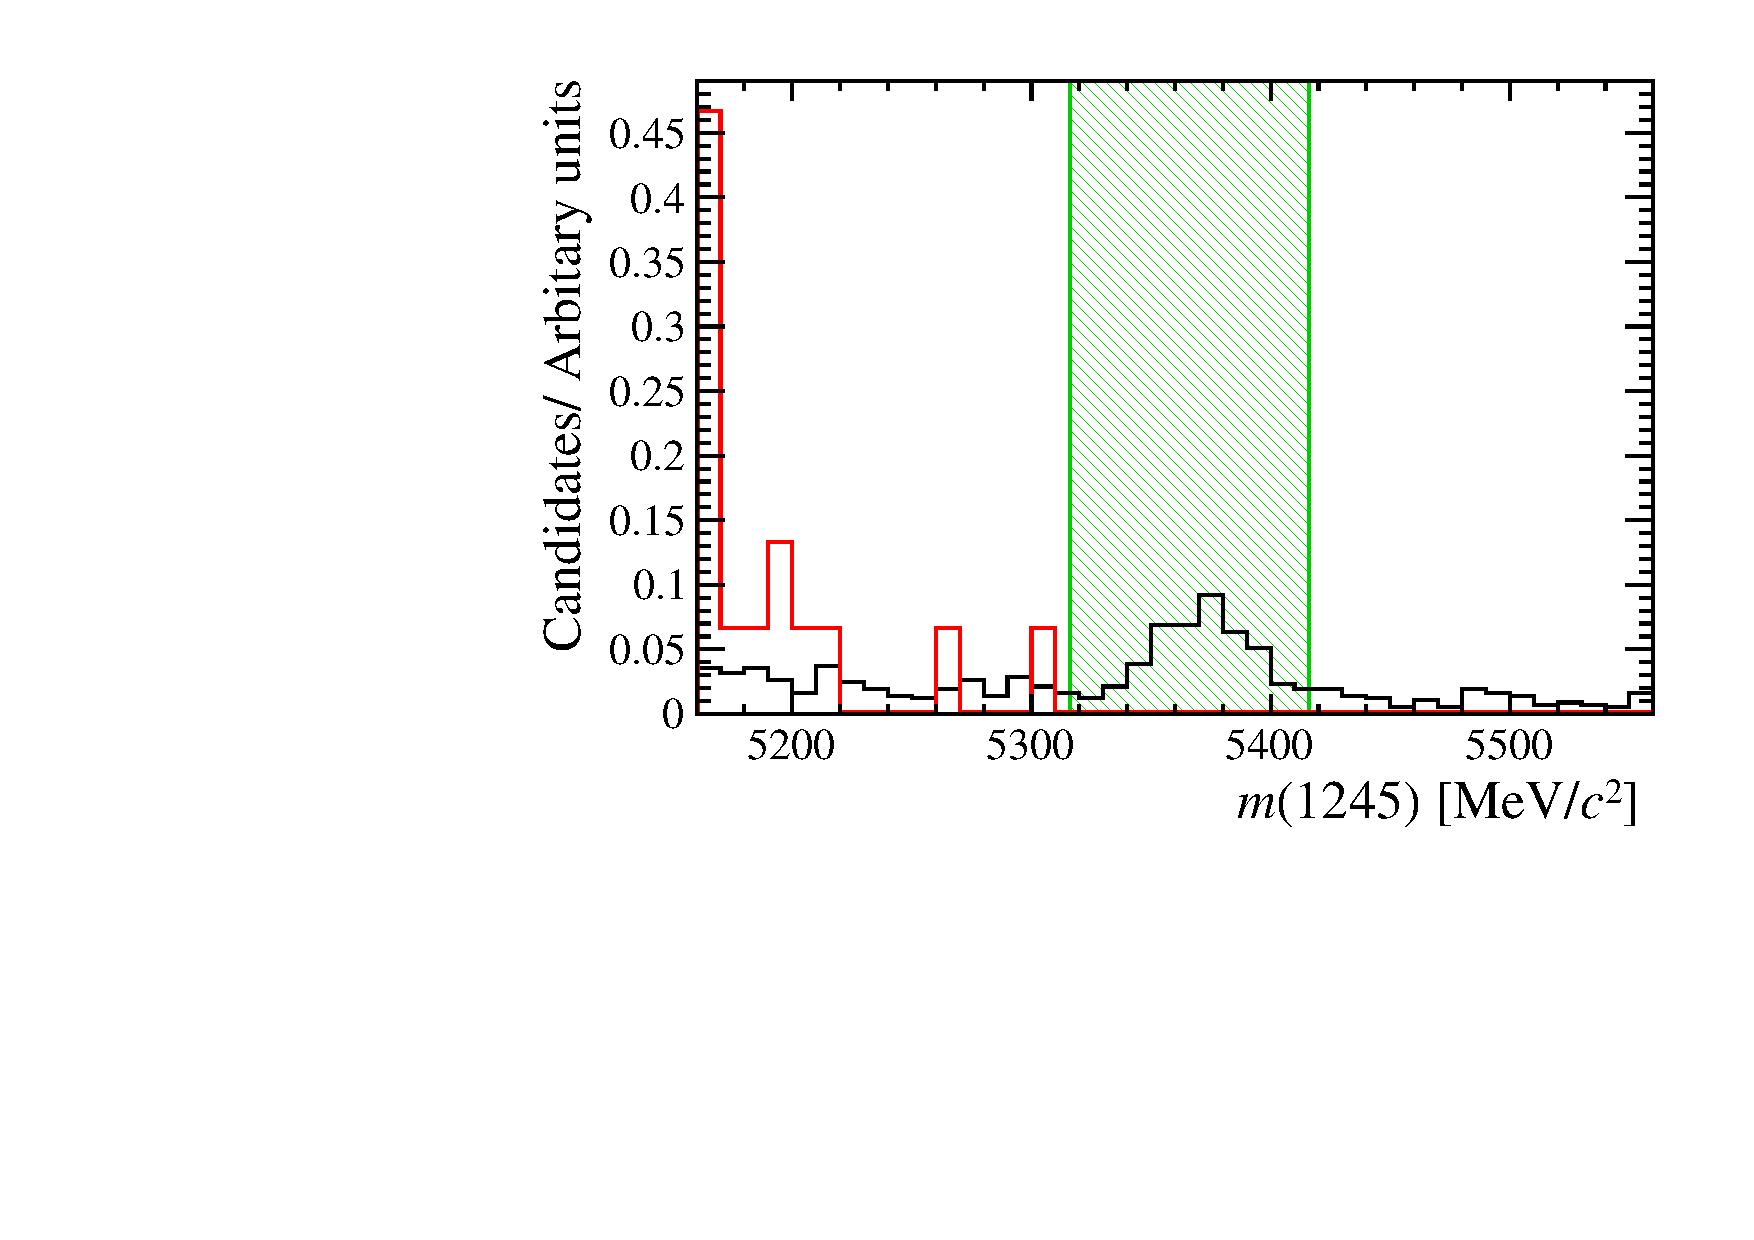
\includegraphics[width=1.0\textwidth]{figs/Selection/Veto_Comparison_B2DsKK_Ds2KKPi_m1245.pdf}
%       \end{subfigure}\\
%       \begin{subfigure}[t]{0.32\textwidth}
%          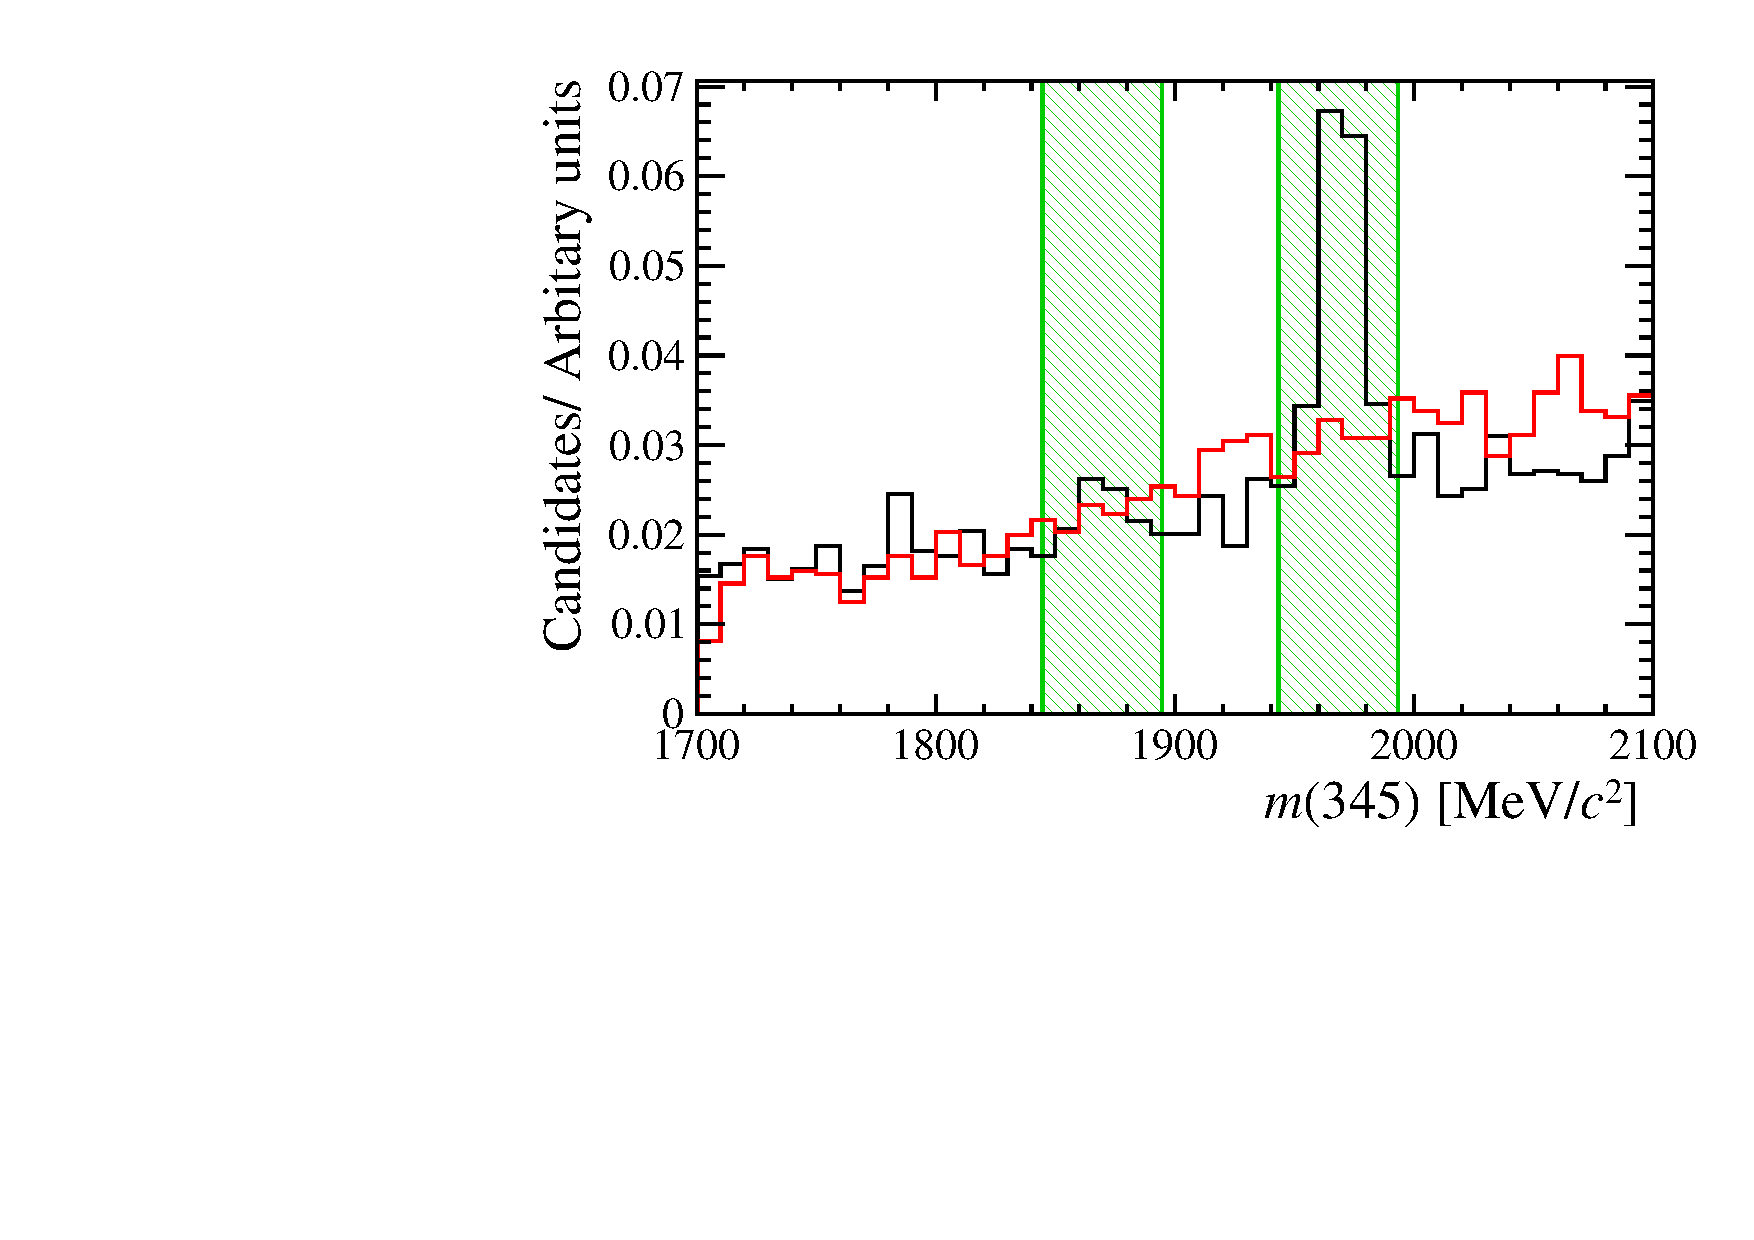
\includegraphics[width=1.0\textwidth]{figs/Selection/Veto_Comparison_B2DsKK_Ds2KKPi_m345.pdf}
%       \end{subfigure}
%       \begin{subfigure}[t]{0.32\textwidth}
%          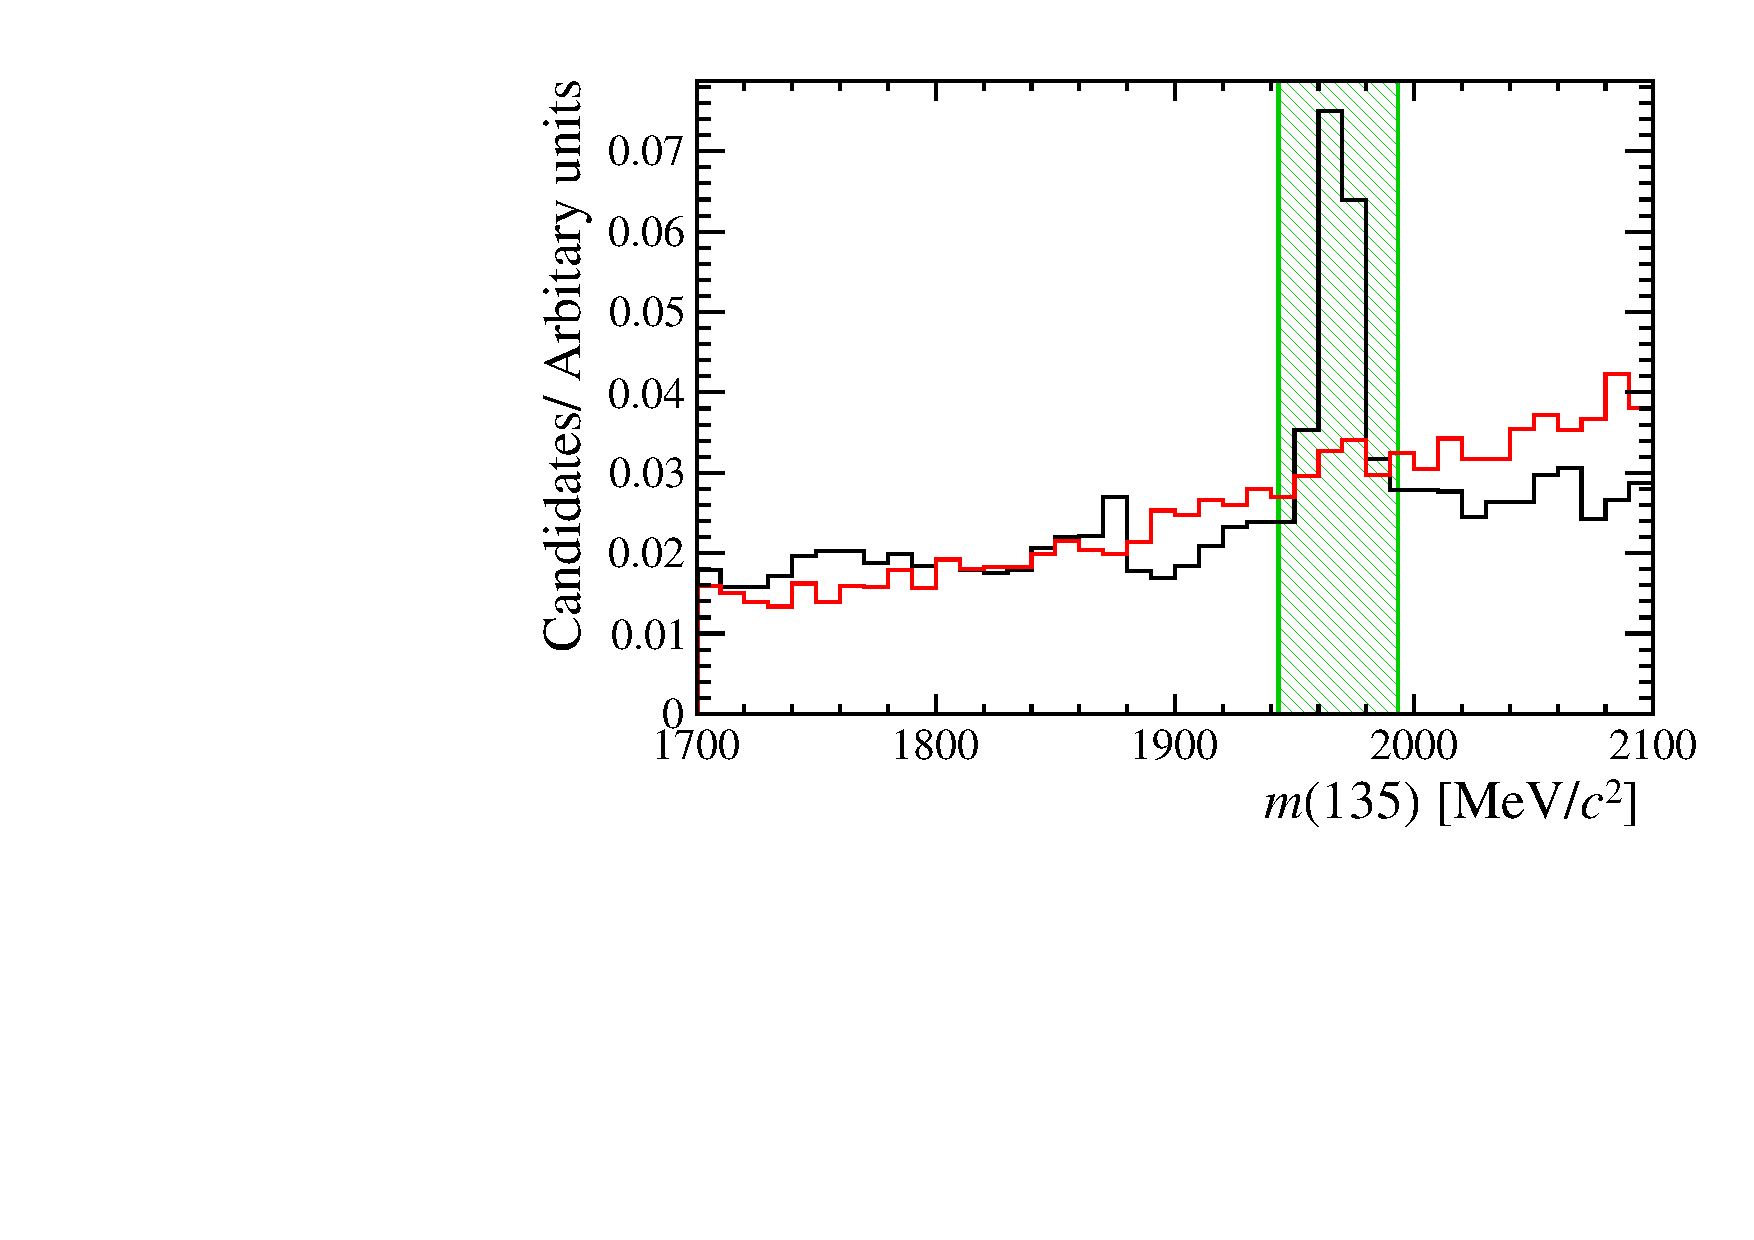
\includegraphics[width=1.0\textwidth]{figs/Selection/Veto_Comparison_B2DsKK_Ds2KKPi_m135.pdf}
%       \end{subfigure}
%       \begin{subfigure}[t]{0.32\textwidth}
%          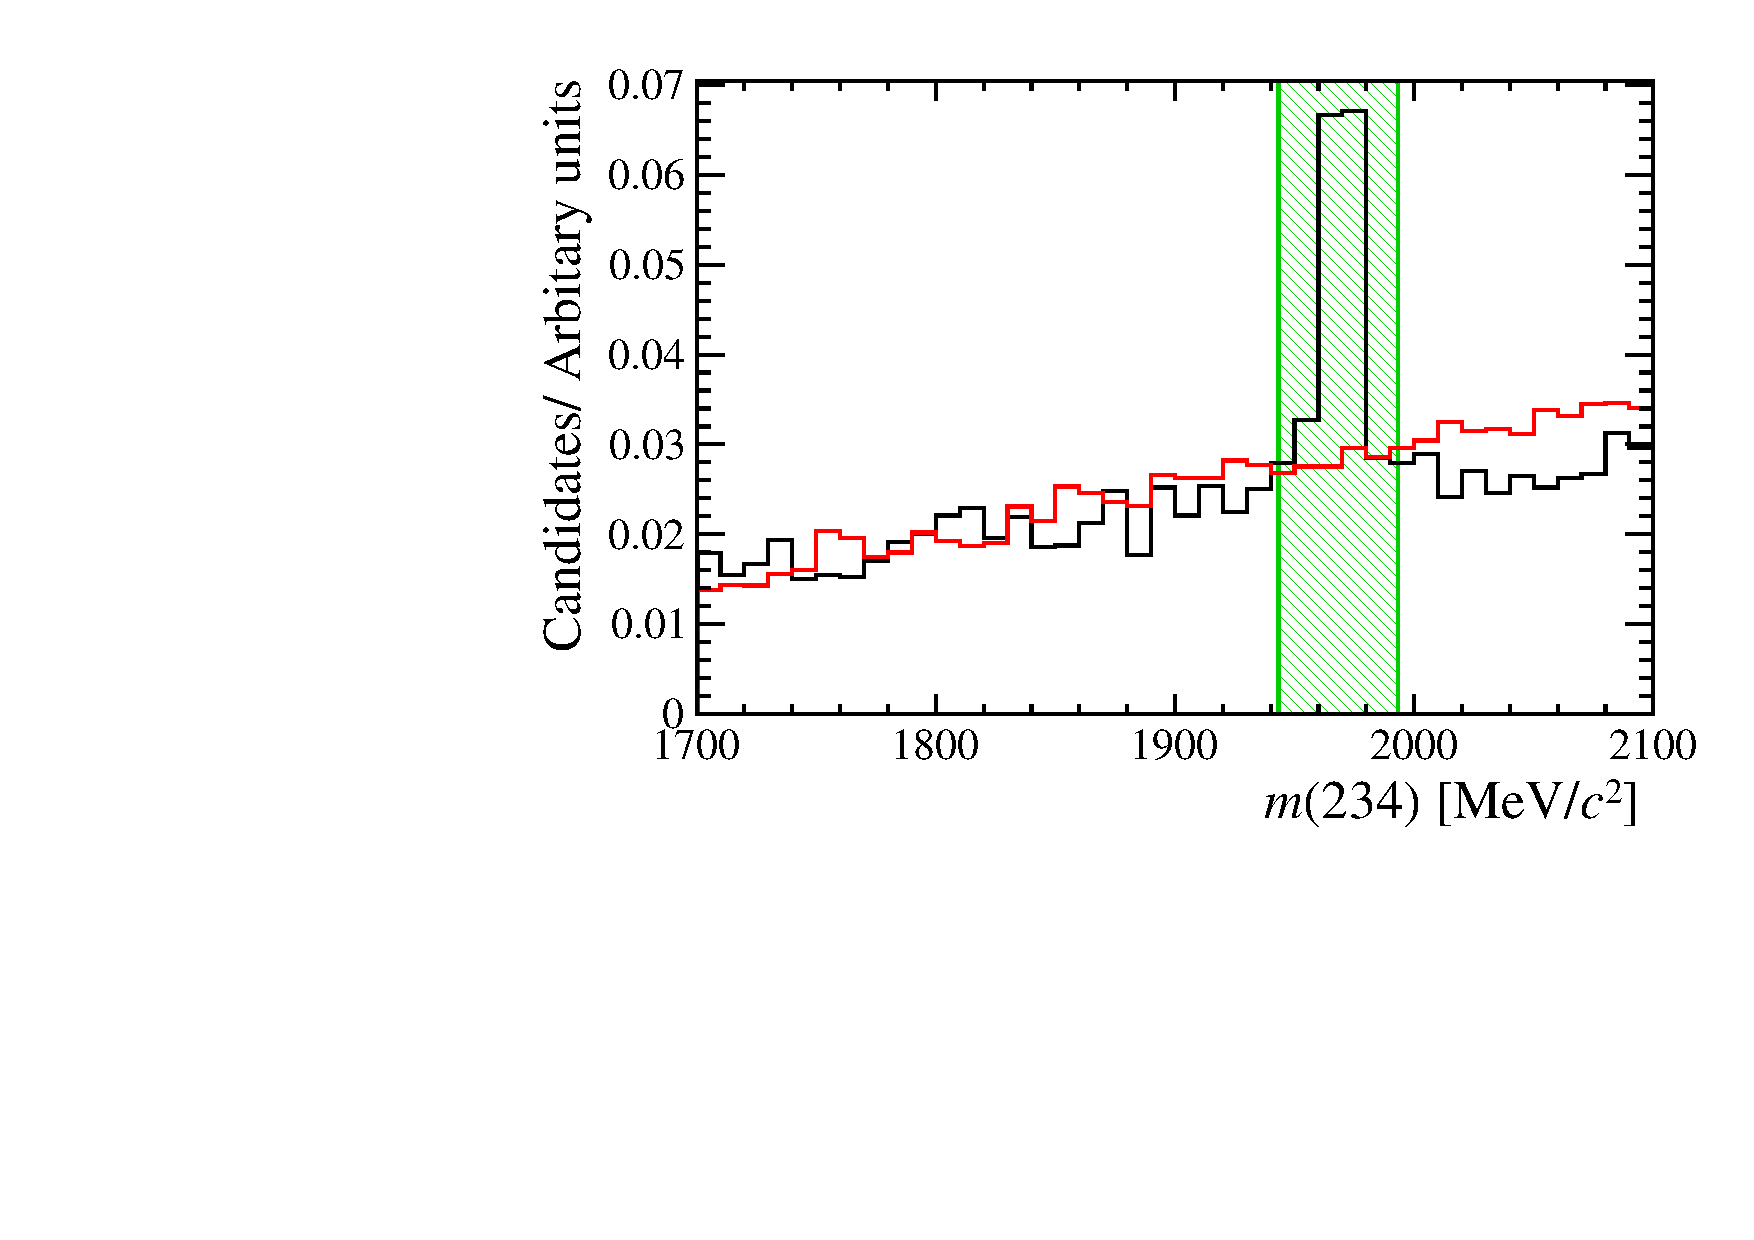
\includegraphics[width=1.0\textwidth]{figs/Selection/Veto_Comparison_B2DsKK_Ds2KKPi_m234.pdf}
%       \end{subfigure}
%    \end{subfigure}

%    \caption{Invariant mass distributions for subsets of decay products for \decay{\Bp}{(\decay{\Dsp}{\Kp\Km\pip})\Kp\Km} decays in data (black) and simulation (red). The green region show the regions removed by the vetoes listed in Sec~\ref{sec:kinematicvetos}.}
%    \label{fig:invariantmassvetoes_DsKK}   
% \end{figure}
% %%%%%%%%%%%%%%%%%%%%%%%%%%%%%%%%%%%%%%%%%%%%%%%%%%%%%%%%%%
 
Another set of vetoes rejects decays where the tracks forming the \Dsp candidate originate from an excited charged charm meson decay, for example $\decay{\Dstarp}{(\decay{\Dz}{h^{+}h'^{-}}) \pip}$. By requiring $\Delta m = m(h^{+}h'^{-}\pip)-m(h^{+}h'^{-}) > 150 \mevcc$ decays of this type are efficiently removed. These are applied to both the signal and normalisation modes for all \Dsp decays. 


\subsection{Normalisation mode veto}
\label{sec:normvetos}

In the search for \decay{\Bp}{\Dsp\Kp\Km} decays, the entire $m(\Kp\Km)$ phasespace is used. This ranges from the \Kp\Km mass threshold at around $990\mevcc$ to the kinematic limit at $m(\Bp) - m(\Dsp) = 3300\mevcc$. This range is wide enough to include the mass of the \Dzb meson, $m(\Dz) = 1864 \mevcc$. Consequently, when inspecting the $m(\Kp\Km)$ spectrum for selected signal candidates there is an excess of events at the \Dz mass. It is necessary to remove these from the signal samples as, unsurprisingly, they result in a peak at the \Bp mass in the $m(\Dsp\Kp\Km)$ spectrum and lead to an incorrect signal yield. As described in Section~\ref{sec:selectionrequirements}, these removed events are used as the normalisation channel for the measurement of \decay{\Bp}{\Dsp\Kp\Km} decays. 
The region affected by the veto $|m(\Kp\Km) - m(\Dzb)| > 25 \mevcc$ is shown in Fig.~\ref{fig:normalisationveto_KK}.

%%%%%%%%%%%%%%%%%%%%%%%%%%%%%%%%%%%%%%%%%%%%%%%%%%%%%%%%%%
\begin{figure}[!h]
   \centering
   \begin{subfigure}[t]{0.49\textwidth}
      \centering
      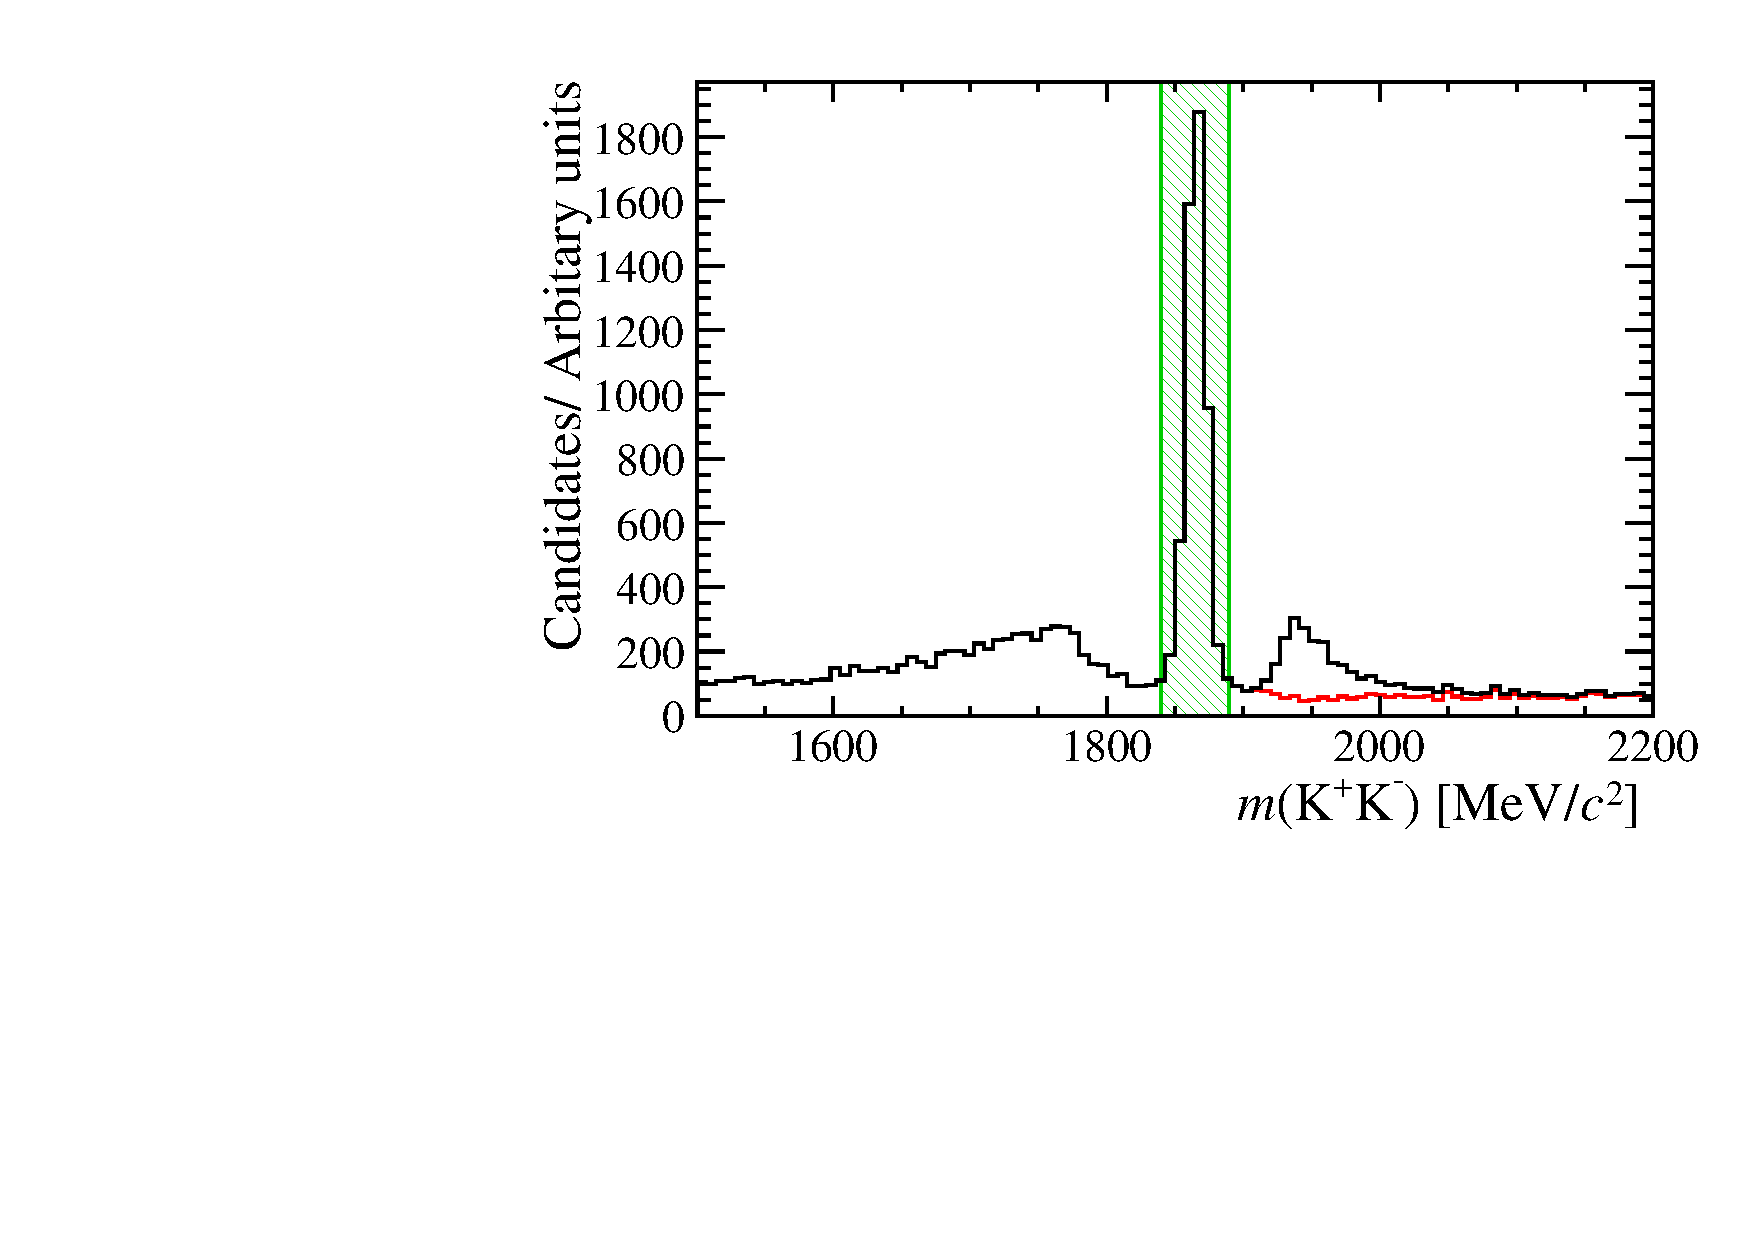
\includegraphics[width=1.0\textwidth]{figs/Selection/D0Veto_Comparison_B2DsKK_Ds2KKPi_Phi_M.pdf}
      \caption{\decay{\Dzb}{\Kp\Km} }
      \label{fig:normalisationveto_KK}
   \end{subfigure}
   \begin{subfigure}[t]{0.49\textwidth}
      \centering
      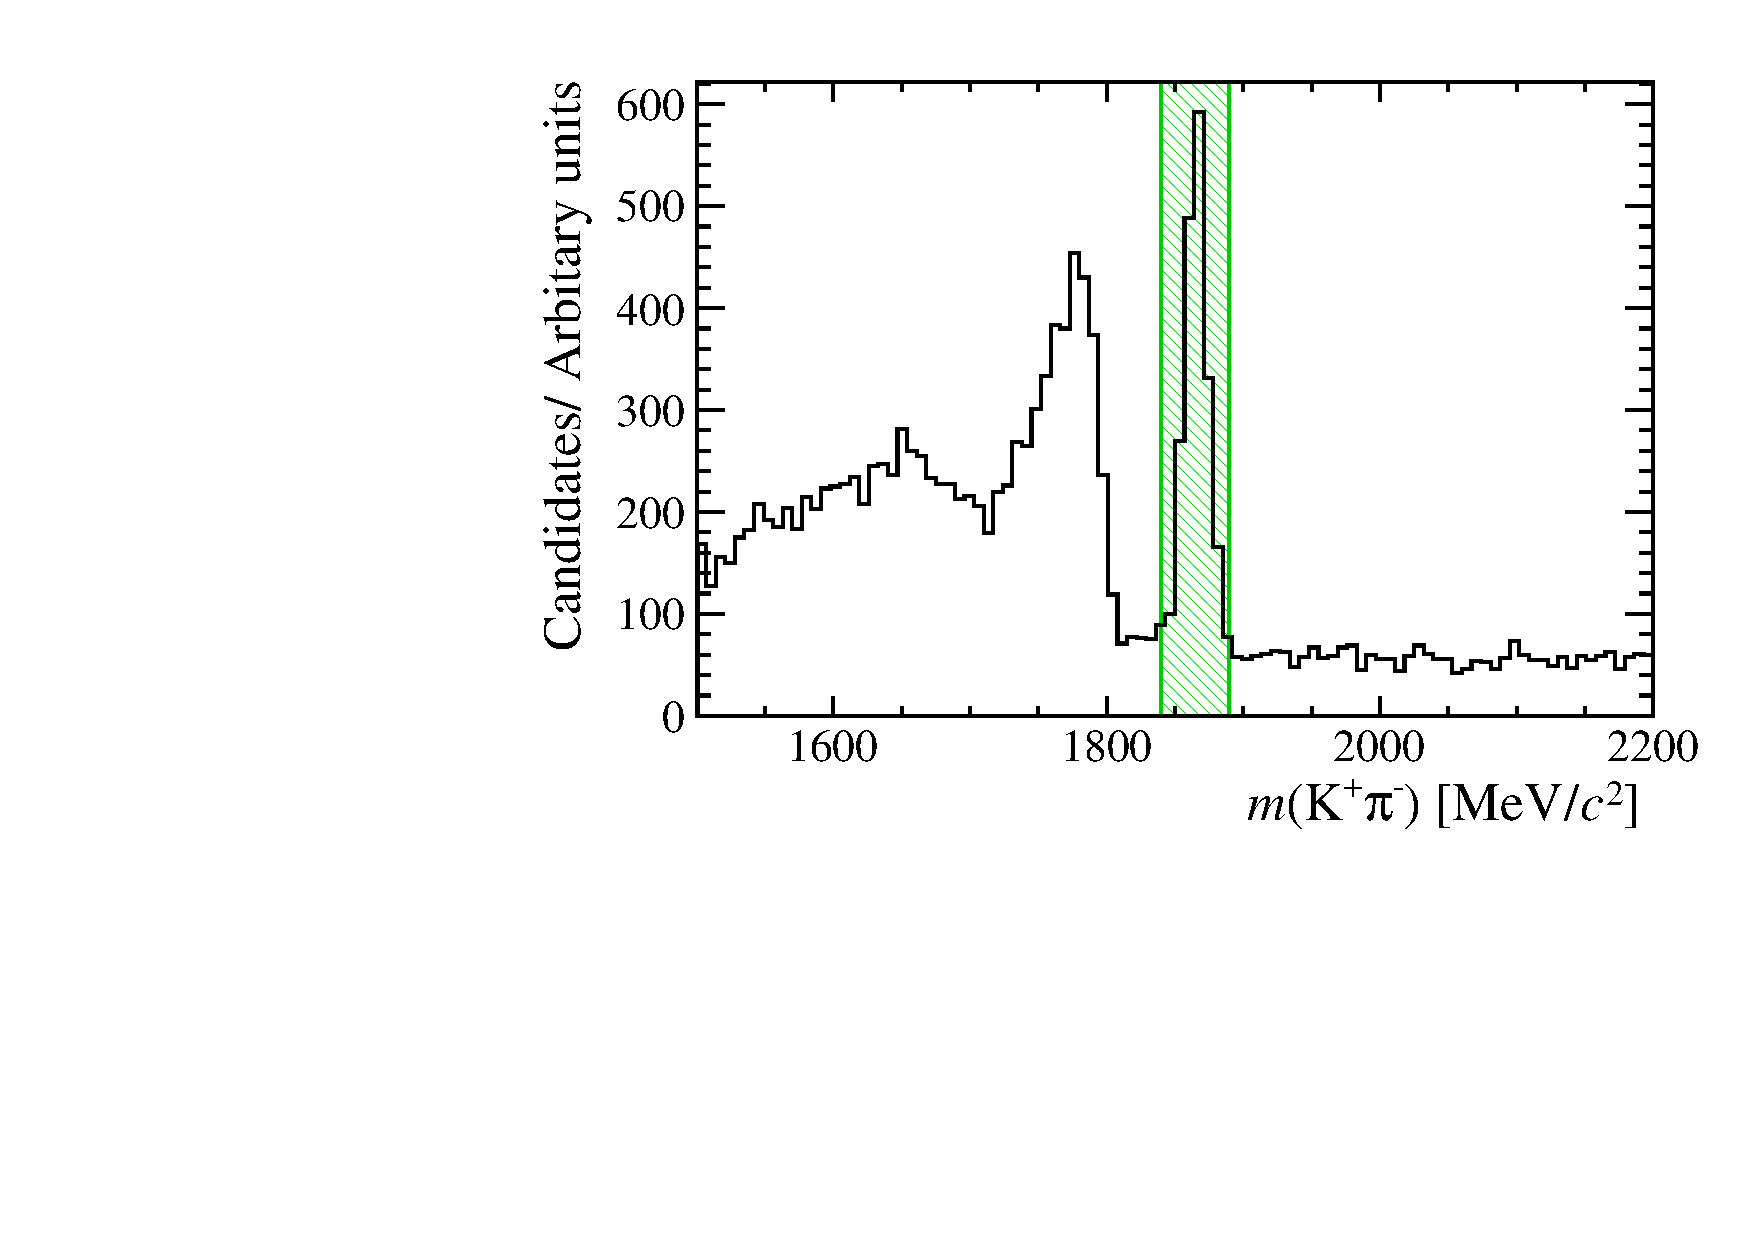
\includegraphics[width=1.0\textwidth]{figs/Selection/D0Veto_Comparison_B2DsKK_Ds2KKPi_Phi_KPi_M.pdf}
      \caption{\decay{\Dzb}{\Kp\pim} }
      \label{fig:normalisationveto_KPi}
   \end{subfigure}
   \caption{The vetoes applied to remove the normalisation channel \decay{\Bp}{\Dsp\Dzb} from the sample of \decay{\Bp}{\Dsp\Kp\Km} decays. Both the correctly reconstructed \decay{\Dzb}{\Kp\Km} (left) and mis-reconstructed \decay{\Dzb}{\Kp\pim} decays (right) are targeted. The effect of the mis-reconstructed \decay{\Dzb}{\Kp\pim} decay veto on the $m(\Kp\Km)$ distribution is shown in red in the left plot.}
   \label{fig:normalisationveto}   
\end{figure}
%%%%%%%%%%%%%%%%%%%%%%%%%%%%%%%%%%%%%%%%%%%%%%%%%%%%%%%%%%


In addition to the correctly reconstructed normalisation channel, the presence of the incorrectly reconstructed \decay{\Bp}{\Dsp(\decay{\Dzb}{\Kp\pim})} decay is observable in Fig.~\ref{fig:normalisationveto_KK}. This appears as smeared out peak to the right of the \Dzb peak. Although the probability of the \pim meson being misidentified as a \Km meson is low for the chosen PID requirements ($\mathcal{O}(1\%)$), the branching fraction for \decay{\Dzb}{\Kp\pim} is larger, leading to the observed excess. It is possible, and necessary, to remove this contribution. The \Kp\Km candidates are reconstructed again, swapping the mass hypothesis of the second track from \Km to \pim. The distribution of these candidates in the vicinity of the \Dzb mass is shown in Fig.~\ref{fig:normalisationveto_KPi}. A distinct peak is observed at the \Dzb mass. This contribution is removed by the requirement $|m(\Kp\pim) - m(\Dzb)| > 25 \mevcc$. The effect of this requirement on the $m(\Kp\Km)$ spectrum is shown by the red line in Fig.~\ref{fig:normalisationveto_KK}, which represents the sample with this veto applied. The \decay{\Bp}{\Dsp(\decay{\Dzb}{\Kp\pim})} background is reduced to a negligible level.

Another structure appears to be present to the left of the \Dzb peak in Fig.~\ref{fig:normalisationveto_KK}. This is likely to be due to \decay{\Dzb}{\Kp\Km X} decays in which one or more particles have not been reconstructed. This partially reconstructed background would not peak at the \Bp mass in the $m(\Dsp\Kp\Km)$ spectrum due to the missing particles, therefore no attempt is made to remove this contribution.


\subsection{Multivariate analysis}
\label{sec:selection_MVA}

Multivariate Analyses (MVAs) are used to help discriminate between genuine \Dsp and \phiz-meson decays and combinations of unrelated tracks. 

In many analyses of \B mesons at \lhcb, it is conventional to train MVAs using simulation samples to represent the signal decays and signal-depleted regions of data to define the background samples. However certain variables, for example particle identification variables, are not perfectly represented in the \lhcb simulations. As a result these variables cannot be used in MVAs using these simulations to define the signal distributions and must be optimised separately.  
To circumvent this issue, an alternative approach has been developed to use large, high-purity data samples as a signal sample to train MVAs, reducing the dependency on simulations. Rather that using a single MVA to select the signal decays, the decay chain is split into the contributing mesons, in this case \Dsp and \phiz, and a MVA trained for each. These intermediate mesons are reconstructed in other \B meson decays with similar topologies for maximum efficacy.   
%These MVAs are trained on data using large samples of \B mesons decays which have similar topologies. 
%This data-driven approach can benefit from an expanded set of variables that are not perfectly represented in simulation, including track quality and particle identification information, in addition to the widely used kinematic and geometric properties.
The method is based on the approach used in Ref.~\cite{LHCb-PAPER-2012-050}, however the choice of input variables has been optimised and training samples expanded to include Run II data.

The sample of \Dsp mesons is obtained from the relatively abundant \decay{\Bsb}{\Dsp\pim} decay. Similarly, the sample of \phiz mesons is obtained from \decay{\Bs}{\jpsi\phiz} decays. Large, high purity samples are reconstructed using similar requirements to those applied in the selection of signal \Dsp and \phiz mesons.
A sample is selected for each of the \Dsp and \phiz-meson decays uses in this analysis, as listed in Table~\ref{tab:mva_modes}. 
The training of separate MVAs for the different \Dsp modes allows the use of particle identification variables that separate kaons and pions to be fully exploited.
The MVA trained using \decay{\Bs}{\jpsi(\decay{\phiz}{\Kp\Km})} decays is used to select both \decay{\phiz}{\Kp}{\Km} and \decay{\Dzb}{\Kp\Km} decays. For the normalisation mode this may be suboptimal, however it ensures the selection of the signal and normalisation channels are almost identical such that the systematic uncertainty in the ratio of efficiencies is minimised.
The samples of \decay{\Bsb}{\Dsp\pim} and \decay{\Bs}{\jpsi\phiz} decays are randomly split into two subsamples. The first is used to train the MVAs and the second is used to determine the efficiency of the selection. To prevent the difference between \phiz and \Dzb decays from affecting the ratio of efficiencies, the normalisation channel MVA efficiency is instead determined from a dedicated sample of \decay{\Dzb}{\Kp\Km} decays as detailed in Table.~\ref{tab:mva_modes}. The \decay{\phiz}{\Kp\Km} MVA is also used to select the \Kp\Km pair in \decay{\Bp}{\Dsp\Kp\Km} decays.
A total of eight MVAs are trained, one for each of the \Dsp and \phiz modes, in both Run I and Run II. Changes to the particle identification variables between the two running periods necessitates separate trainings. 


\begin{table}[h]
\centering
\begin{tabular}{lll}
   \hline
   Sample                    & Mode                       & Use \\ 
   \hline
   \decay{\Bsb}{\Dsp\pim}    & \decay{\Dsp}{\Kp\Km\pip}   & Training, Efficiency \\
   \decay{\Bsb}{\Dsp\pim}    & \decay{\Dsp}{\Kp\pim\pip}  & Training, Efficiency \\
   \decay{\Bsb}{\Dsp\pim}    & \decay{\Dsp}{\pip\pim\pip} & Training, Efficiency \\
   \decay{\Bs}{\jpsi\phiz}   & \decay{\phiz}{\Kp\Km}      & Training, Efficiency \\
   \hline
   \decay{\Bp}{\Dzb\pip}     & \decay{\Dzb}{\Kp\Km}       & Efficiency          \\
   \hline
\end{tabular}

\caption{The decay modes used to train and determine the efficiency of the various MVAs used in this analysis.}
\label{tab:mva_modes}
\end{table}

\subsubsection{Preselection}

Before the samples of \Dsp and \phiz mesons are used to train the MVAs, precautions are taken to ensure the samples are representative of the \decay{\Bp}{\Dsp\phiz} and \decay{\Bp}{\Dsp\Kp\Km} signal decays. The \decay{\Bsb}{\Dsp\pim} and \decay{\Bs}{\jpsi\phiz} decays are selected using a similar procedure to the signal modes. Firstly, \emph{Stripping Lines} reconstruct the candidates. The \decay{\Bsb}{\Dsp\pim} decays are built using the same software module as the signal and normalisation channel. Therefore, the selection requirements for \Dsp candidates in \decay{\Bsb}{\Dsp\pim} decays are identical to those for the signal (Appendix~\ref{ch:appendix_selection}).
The \decay{\Bs}{\jpsi\phiz} decays are reconstructed using \decay{\jpsi}{\mup\mun} decays, therefore they are built using a different software module as the final state is not fully hadronic. As such there are some differences in the selection requirements for the \phiz mesons from the two sources. In general the selection requirements for the \decay{\Bs}{\jpsi\phiz} channel are looser as the presence of the muons allows an efficient triggering without the need to make tight selections on the \Kp\Km pair. 
A full comparison of the relevant quantities are detailed in Appendix~\ref{sec:app_mva_preselection}.

%A direct comparison of the relevant quantities are listed in Table~\ref{tab:strippingrequirments_phi}.


% \begin{table}[h]
% \centering
% \begin{tabular}{ l l l l }
% \hline
% Particle       & Quantity                       &  Signal                              & Control                                 \\  
% \hline
% \phiz          & Mass minimum                   &  $870\mevcc$                         & $980\mevcc$ \\ 
%                & Mass maximum                   &  $1170\mevcc$                        & $1050\mevcc$ \\ 
%                & Transverse Momentum            &  -                                   & $\pt > 500 \mevc$                       \\  
%                & Products \pt scalar sum        &  $\sum{|\pt|} > 1000 \mevc$          &  -                                      \\  
%                & $\text{DOCA}(\Kp,\Km)$         &  $ < 0.5\mm$     &  -                                      \\  
%                & Direction angle                &  $\cos{\theta}>0$                    &  -                                      \\  
%                & Vertex quality                 &  $\chi^{2}/N_{\text{DOF}} < 16$      & $\chi^{2}/N_{\text{DOF}} < 25$          \\   
%                & Flight distance significance   &  $\chi^{2}_{\text{FD} }  > 16$       &  -                                      \\ 
% \hline
% \Kpm           & Track quality                  &  $\chi^{2}/N_{\text{DOF}}<4.0$       &  $\chi^{2}/N_{\text{DOF}}<5.0$          \\  
%                & Transverse momentum            &  $\pt > 100 \mevc$                   &  -                                      \\  
%                & Momentum                       &  $\ptot > 1000 \mevc$                &  -                                      \\  
%                & Impact parameter significance  &  $\chi^{2}_{\text{IP}} > 4$          &  -                                      \\  
%                & Ghost track probability        &  $P_{\text{Ghost}} < 0.4$            &  -                                      \\
%                & Particle identification        &  $\text{PIDK}>-10$                   & $\text{PIDK}>0$                         \\ 
% \hline
% \end{tabular}

% \caption{The \emph{Stripping Line} requirements for \decay{\phiz}{\Kp\Km} candidates in the signal and MVA training (control) mode selection. All requirements are looser for the control channel with the exception of the particle identification requirements.}
% \label{tab:strippingrequirments_phi}
% \end{table}

% The difference in the two selections could be potentially biasing when calculating the efficiency of the MVA, therefore the requirements are tightened on the half of the \decay{\Bs}{\jpsi\phiz} sample used to calculate the efficiency. The looser set of requirements are still used when training the MVA methods to maximise the sample sizes to help prevent overtraining. When training the MVAs the \phiz meson invariant mass sidebands in the \decay{\Bs}{\jpsi\phiz} sample are used as the background sample. It was found that using the tighter set of requirements led to a negligible amount of background candidates, resulting in overtraining. 


% The second step of preselection aims to apply the same sequence of requirements to the modes used to train the MVAs as are applied to the signal and normalisation before the MVAs are applied. These are made up of the same trigger, background veto and PID requirements.
% For \Dsp candidates from \decay{\Bsb}{\Dsp\pim} decays, the \Bsb meson is required to either be \texttt{TOS} with respect to the \texttt{L0Hadron} trigger or \texttt{TIS} with respect to \texttt{L0Global} as with the signal. The \Bsb candidates are then required to be \texttt{TOS} with respect to the same \hltone and \hlttwo triggers as used with the signal modes.

% For the \decay{\Bs}{\jpsi\phiz} candidates, a large fraction are triggered due to the muons from the \jpsi decay. To ensure the sample is reflective of the signal decays the \Bs meson is required to be \texttt{TOS} with respect to the \texttt{L0Hadron} trigger or \texttt{TIS} with respect to \texttt{L0Global}. This effectively excludes events that have been selected solely due to muons initiating the muon hardware trigger. This consequently results in a large decrease in the available statistics.

% As shown in Table~\ref{tab:strippingrequirments_phi}, the MVA training mode has tighter particle identification requirements than the signal mode. Particle identification plays a crucial role in the efficacy of the MVA methods, therefore the signal PID requirements for the \phiz-meson decay products are tightened accordingly as discussed in Section~\ref{sec:pidrequirements}.

% Finally, the same misidentified \D and \Lc hadron vetoes as detailed in Section~\ref{sec:pidvetos} are applied to the \decay{\Bsb}{\Dsp\pim} sample. These help to ensure the samples of \Dsp candidates are free from contamination.


\subsubsection{Background subtraction}
\label{sec:MVAbackgroundsubtraction}
%% Describe fits, sWeights and signal/background samples
In order to use the \decay{\Bs}{\jpsi\phiz} and \decay{\Bsb}{\Dsp\pim} samples to train MVAs, background subtracted distributions must be obtained for the variables used to discriminate the signal from backgrounds.  Firstly, unbinned extended maximum likelihood fits are performed to the \Dsp and \phiz invariant mass distribution in order to determine the yield of \Dsp and \phiz candidates respectively. 
Maximum likelihood fits determine the values of the signal and background yields for which the given data set was most likely. The likelihood, $\mathcal{L}$, is constructed from the probability density functions (PDFs) for the fit model, $F(m,\vec{p})$, for each entry $i$ in the data set. The PDF for each entry is evaluated at the corresponding value of the invariant mass, $m = m_{i}$, such that $\mathcal{L}$ is just a function of the PDF parameters, $\vec{p}$,
\begin{equation}
\mathcal{L}(\vec{p}) = \prod_{i}^{N} F(m=m_{i},\vec{p}).
\end{equation}

The maximum value of $\mathcal{L}(\vec{p})$ is achieved for the set of PDF parameters for which the data was most likely. 
It is computationally beneficial to instead compute the negative log-likelihood (NLL) rather than the likelihood directly, as addition is less intensive than multiplication. The NLL,
\begin{equation}
-\log\mathcal{L}(\vec{p}) = -\sum_{i}^{N} \log F(m=m_{i},\vec{p}),
\end{equation}
is then minimised with respect to the PDF parameters.

This likelihood can be \emph{extended} to allow the total yield attributed to the PDF to be determined as a parameter as well. This is nessesary to determine the yields of both signal and background contributions ($n_{\text{S}}$ and $n_{\text{B}}$).
The likelihood is multiplied by the Poisson probability density for measuring $n = n_{\text{S}} + n_{\text{B}}$ events, 
\begin{equation}
\mathcal{L}(n,\vec{p}) = \frac{n^{N}e^{-n}}{N!}\prod_{i}^{N} F(m=m_{i},\vec{p}) = \frac{e^{-n}}{N!}\prod_{i}^{N} n F(m=m_{i},\vec{p}).
\end{equation}

The extended NLL becomes 
\begin{equation}
-\log\mathcal{L}(n,\vec{p}) = -\sum_{i}^{N} \log n F(m=m_{i},\vec{p}) + n + \log N!.
\end{equation}
The $\log N!$ term can be ignored as it is a constant.
In general, a fit model can be constructed from an arbitrary number of species, $N_{\text{s}}$, each with PDF $f_{j}(m=m_{i},\vec{p})$ and yield $n_{j}$   
\begin{equation}
-\log\mathcal{L}(n_{j},\vec{p}) = -\sum_{i}^{N} \log \sum^{N_{\text{s}}}_{j} n_{j} f_{j}(m=m_{i},\vec{p}) + \sum_{j}^{N_{\text{s}}}n_{j}  + \log N!.
\end{equation}
In this instance the fit model is constructed from the signal and background contributions 
\begin{equation}
n F(m| n_{\text{S}},n_{\text{B}},\vec{p'},\vec{p''}) = n_{\text{S}} f(m|\vec{p'}) + n_{\text{B}} g(m|\vec{p''}),
\end{equation}
where $n_{\text{S}}$ and $n_{\text{B}}$ are the signal and background yields, $f$ and $g$ are the PDFs for the signal and background respectively, and $\vec{p'}$ and $\vec{p''}$ represent the parameters controlling the PDF shapes.
After the extended maximum likelihood fits have been performed and the yields established, the subtraction of candidates attributed to the background component is performed using the \sPlot technique~\cite{Pivk:2004ty}.
The \sPlot method assigns weights for each species in the fit model, namely signal and background.  
The weights, $W_{k}$, for species $k$ are determined as a function of the discriminating variable, $m$,
\begin{equation}
W_{k}(m) = \frac{\sum_{j}^{N_{\text{s}}} V_{kj} f_{j}(m) }{ \sum_{l}^{N_{\text{s}}} n_{l} f_{l}(m)},
\end{equation}
where $V_{nj}$ is the inverse covariance matrix of the negative log likelihood,
\begin{equation}
V^{-1}_{kj} = \frac{  \partial^2 (-\log{\mathcal{L}} ) }{  \partial n_{k} \partial n_{j}}.
\end{equation}
These are assigned to each event in the data set and are only dependent on the value of the fitted variable, in this case \phiz or \Dsp mass. When plotting other, uncorrelated variables and weighting each event accordingly, the contribution from each component in the fit can be extracted.

%% Fit model
For both \decay{\Bs}{\jpsi\phiz} and \decay{\Bsb}{\Dsp\pim} decays, simple fit models are found to be sufficient when performing the \sPlot technique, as detailed in Appendix~\ref{sec:app_mva_fit_models}.
% For each mode the signal components are modelled with a single Gaussian probability density function
% \begin{equation}
% f(m|\mu,\sigma) = \frac{1}{\sqrt{2\pi\sigma^{2}}} \times e^{-\frac{(m-\mu)^{2}}{2\sigma^{2}}}, 
% \end{equation}
% where $\mu$ and $\sigma$ are the mean and width of the Gaussian distribution and $m$ is the observable invariant mass. The parameters $\mu$ and $\sigma$ are allowed to vary freely.
% The background contributions to the \decay{\phiz}{\Kp\Km} decays are modelled using a Chebychev polynomial with two degrees of freedom
% \begin{equation}
% g(m|a,b) = a\times(2m^{2}-1) + b\times m + 1,
% \end{equation}
% where $a$ and $b$ are parameters that can vary freely and $m$ is the observable invariant mass. 
% The \phiz-meson mass is close to the threshold for \Kp\Km pair production so this parametrisation has sufficient freedom to successfully  model the increasing background shape.
% The background contribution to all three \Dsp decays are modelled using exponential functions with a single degree of freedom controlling the effective slope
% \begin{equation}
% g(m|c) = e^{-m\times c},
% \end{equation}
% where $c$ is a freely varying parameter and $m$ is the observable invariant mass.
% The fits to the \phiz and \Dsp meson masses in the \decay{\Bs}{\jpsi\phiz} and \decay{\Bsb}{\Dsp\pim} samples are performed separately for each year of data taking and polarity of the \lhcb dipole magnet. These distributions are shown in Fig.~\ref{fig:mvatrainingsamples} for each of the \phiz and \Dsp decay modes.
% The yields of candidates in each of the subsamples are tabulated in Table~\ref{table:mva_training_yields}, along with the totals for each mode. 


% %%%%%%%%%%%%%%%%%%%%%%%%%%%%%%%%%%%%%%%%%%%%%%%%%%%%%%%%%%
% \begin{figure}[!h]
%    \centering
%    \begin{subfigure}[t]{0.4\textwidth}
%       \centering
%       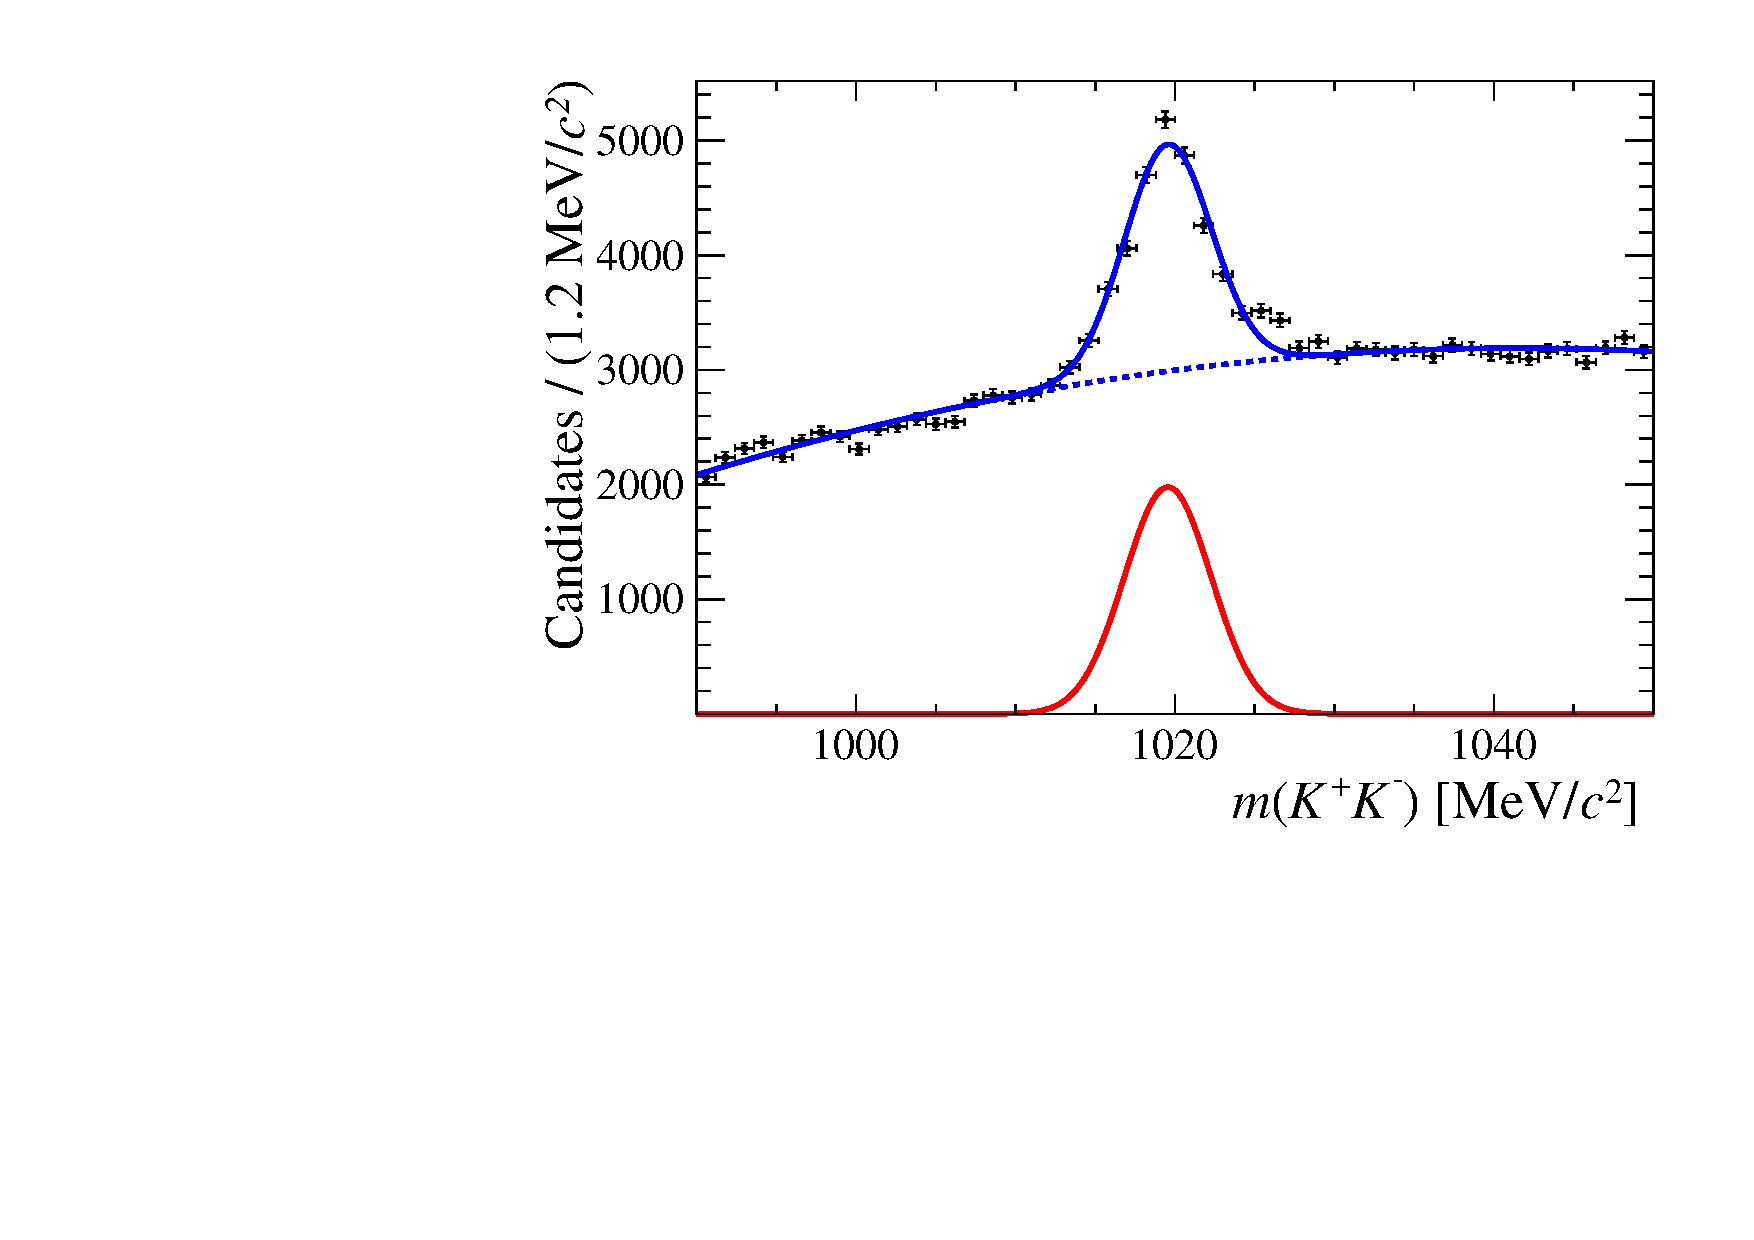
\includegraphics[width=1.0\textwidth]{figs/Selection/Fit_Data_Bs2JpsiPhi_Jpsi2MuMu_Phi2KK_2016_MagDown.pdf}
%       \caption{\decay{\phiz}{\Kp\Km} MagDown}
%    \end{subfigure}
%    \begin{subfigure}[t]{0.4\textwidth}
%       \centering
%       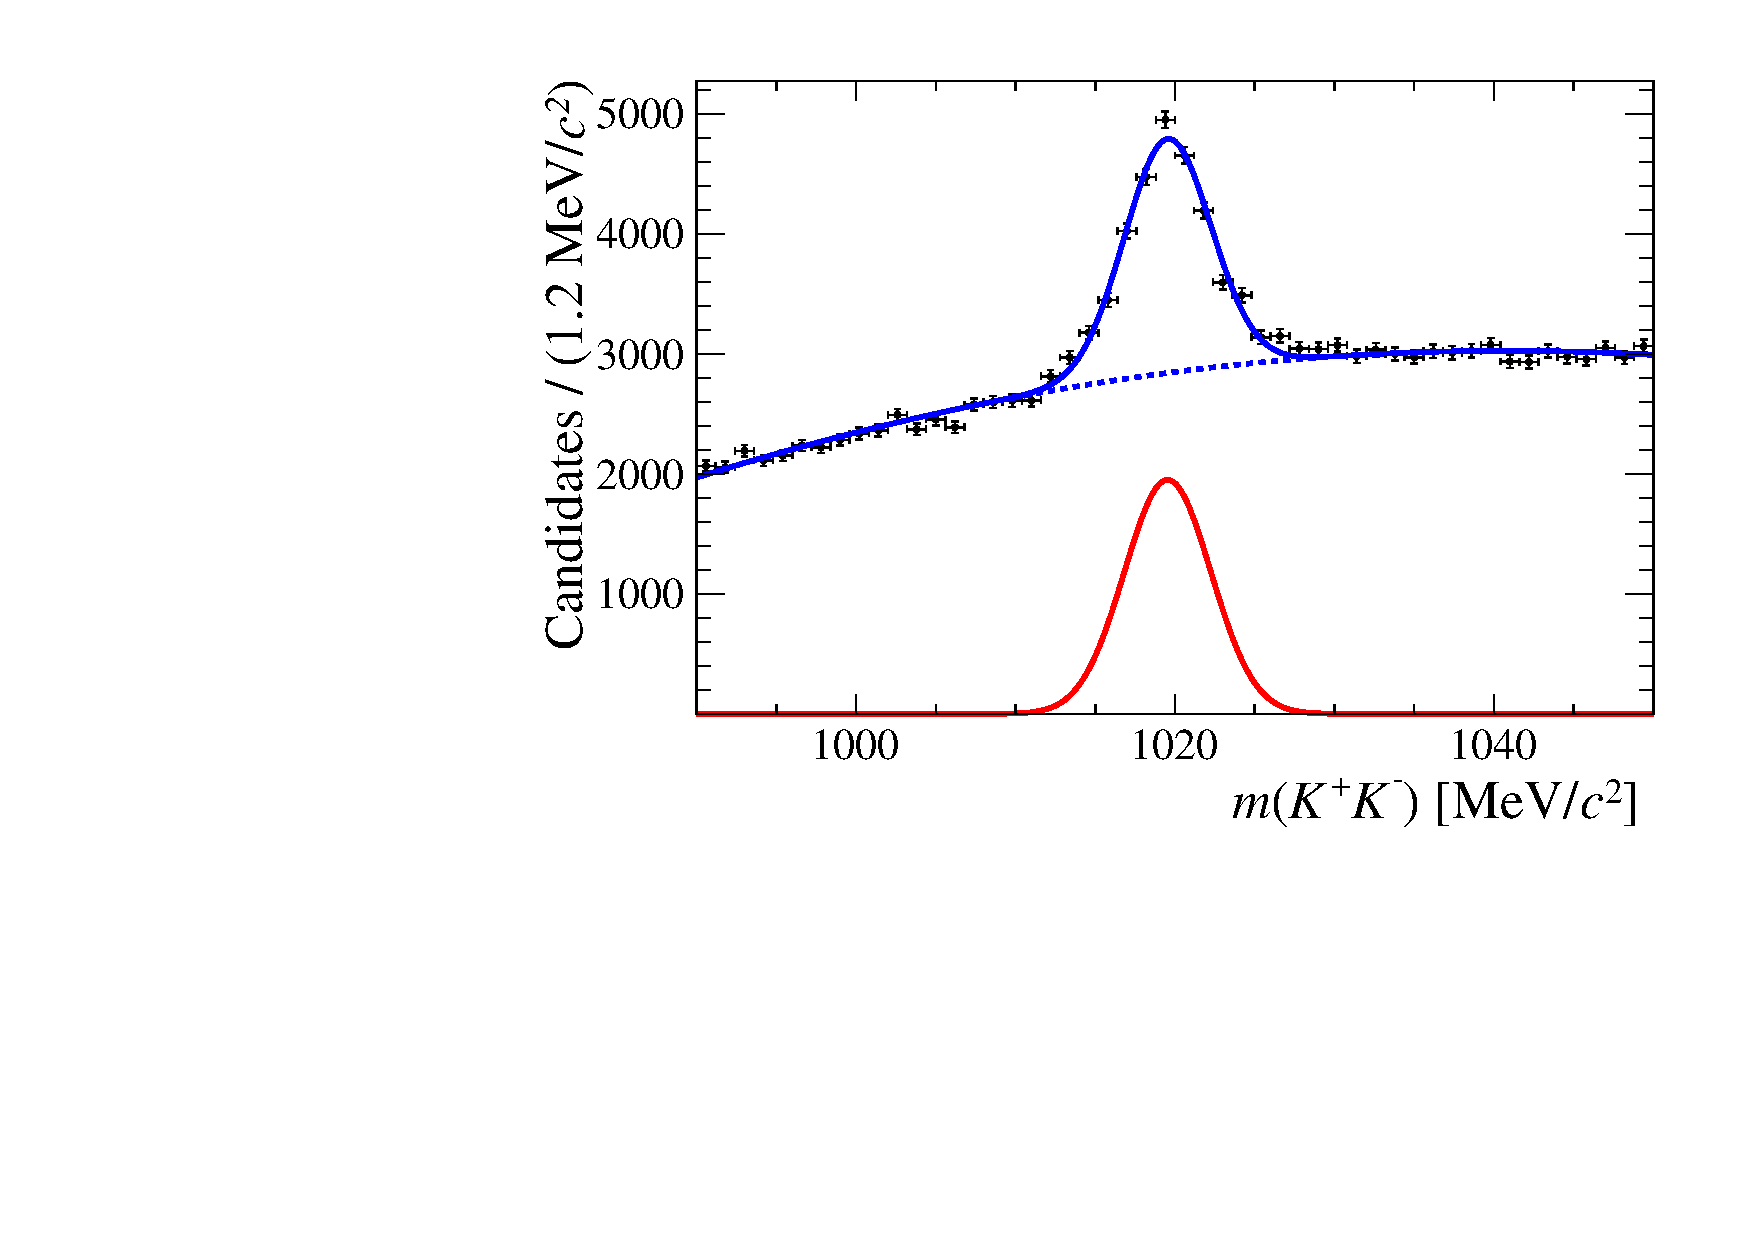
\includegraphics[width=1.0\textwidth]{figs/Selection/Fit_Data_Bs2JpsiPhi_Jpsi2MuMu_Phi2KK_2016_MagUp.pdf}
%       \caption{\decay{\phiz}{\Kp\Km} MagUp}
%    \end{subfigure}\\
%    \begin{subfigure}[t]{0.4\textwidth}
%       \centering
%       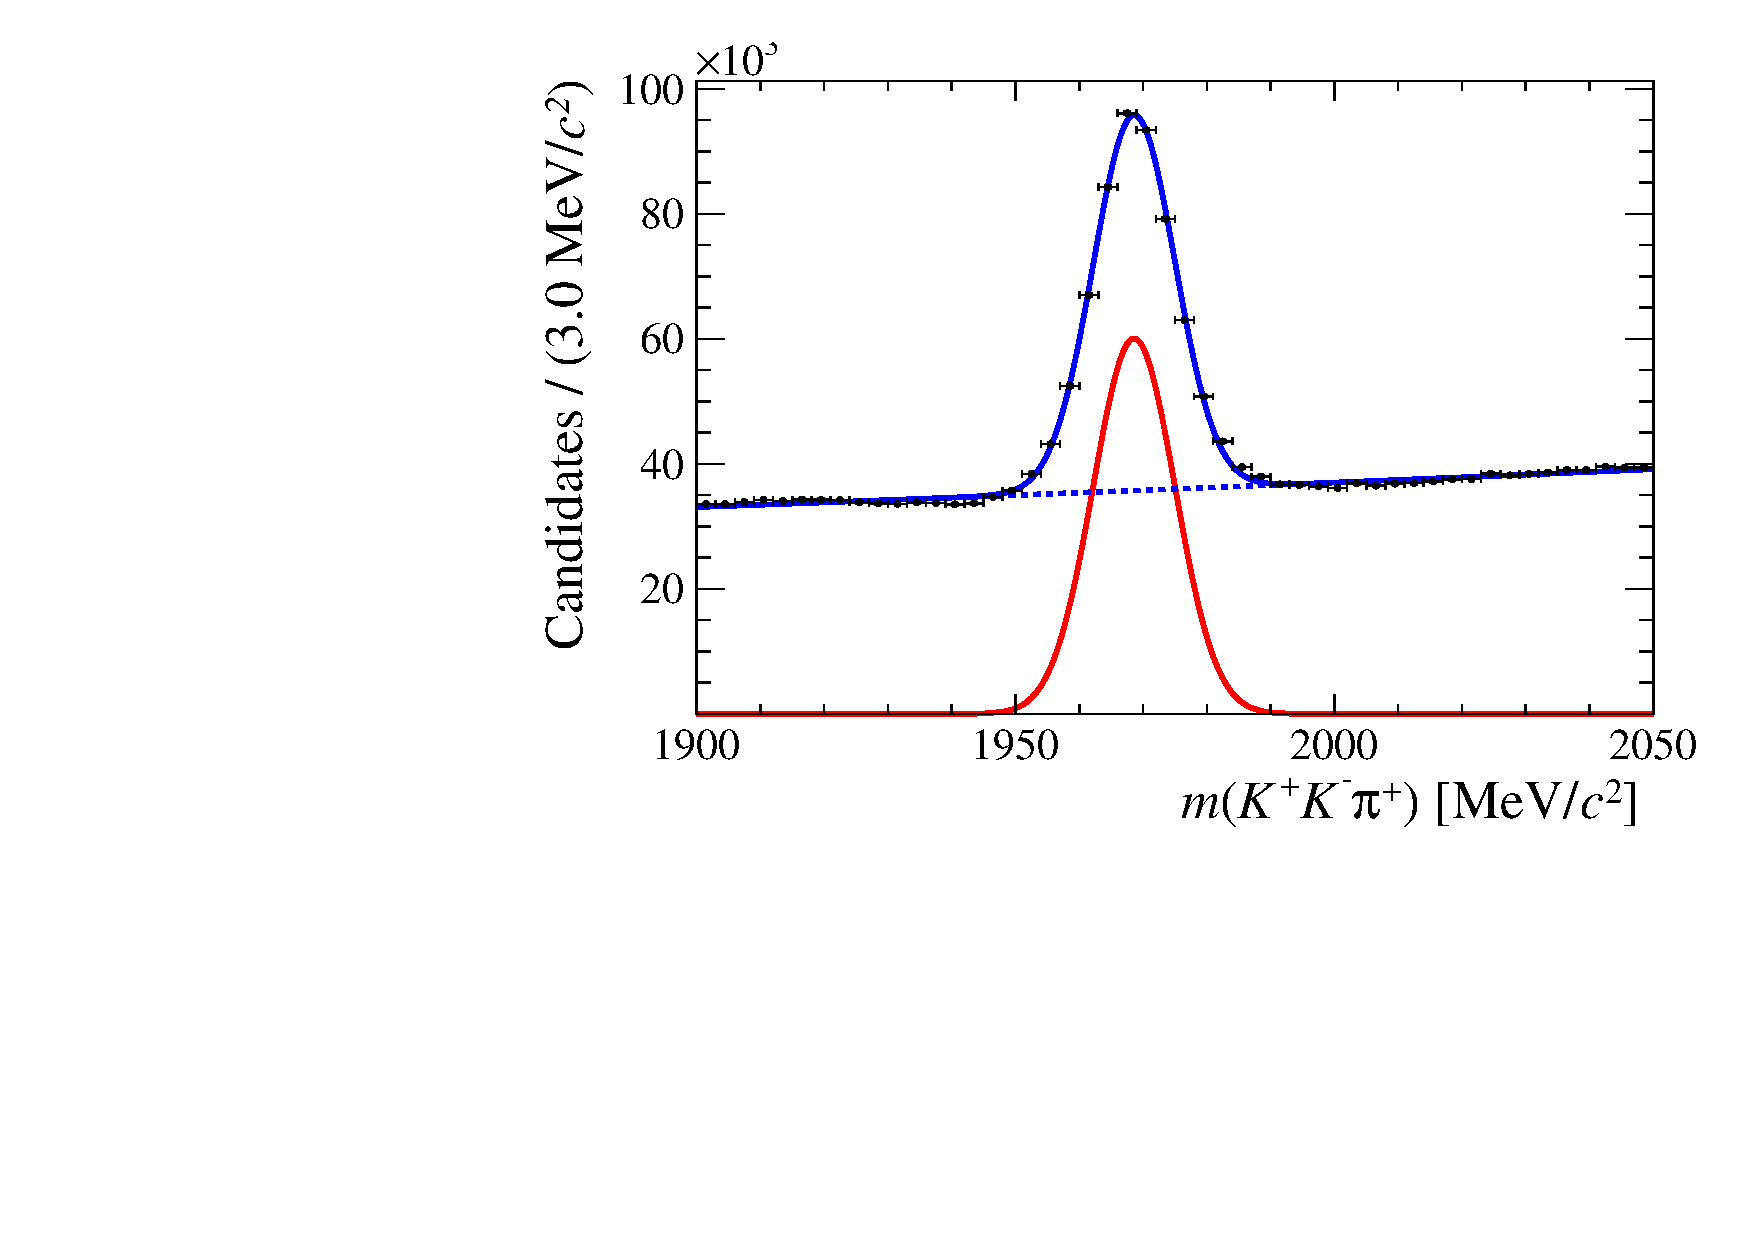
\includegraphics[width=1.0\textwidth]{figs/Selection/Fit_Data_Bs02DsPi_Ds2KKPi_2016_MagDown_PreSel.pdf}
%       \caption{\decay{\Dsp}{\Kp\Km\pip} MagDown}
%    \end{subfigure}
%    \begin{subfigure}[t]{0.4\textwidth}
%       \centering
%       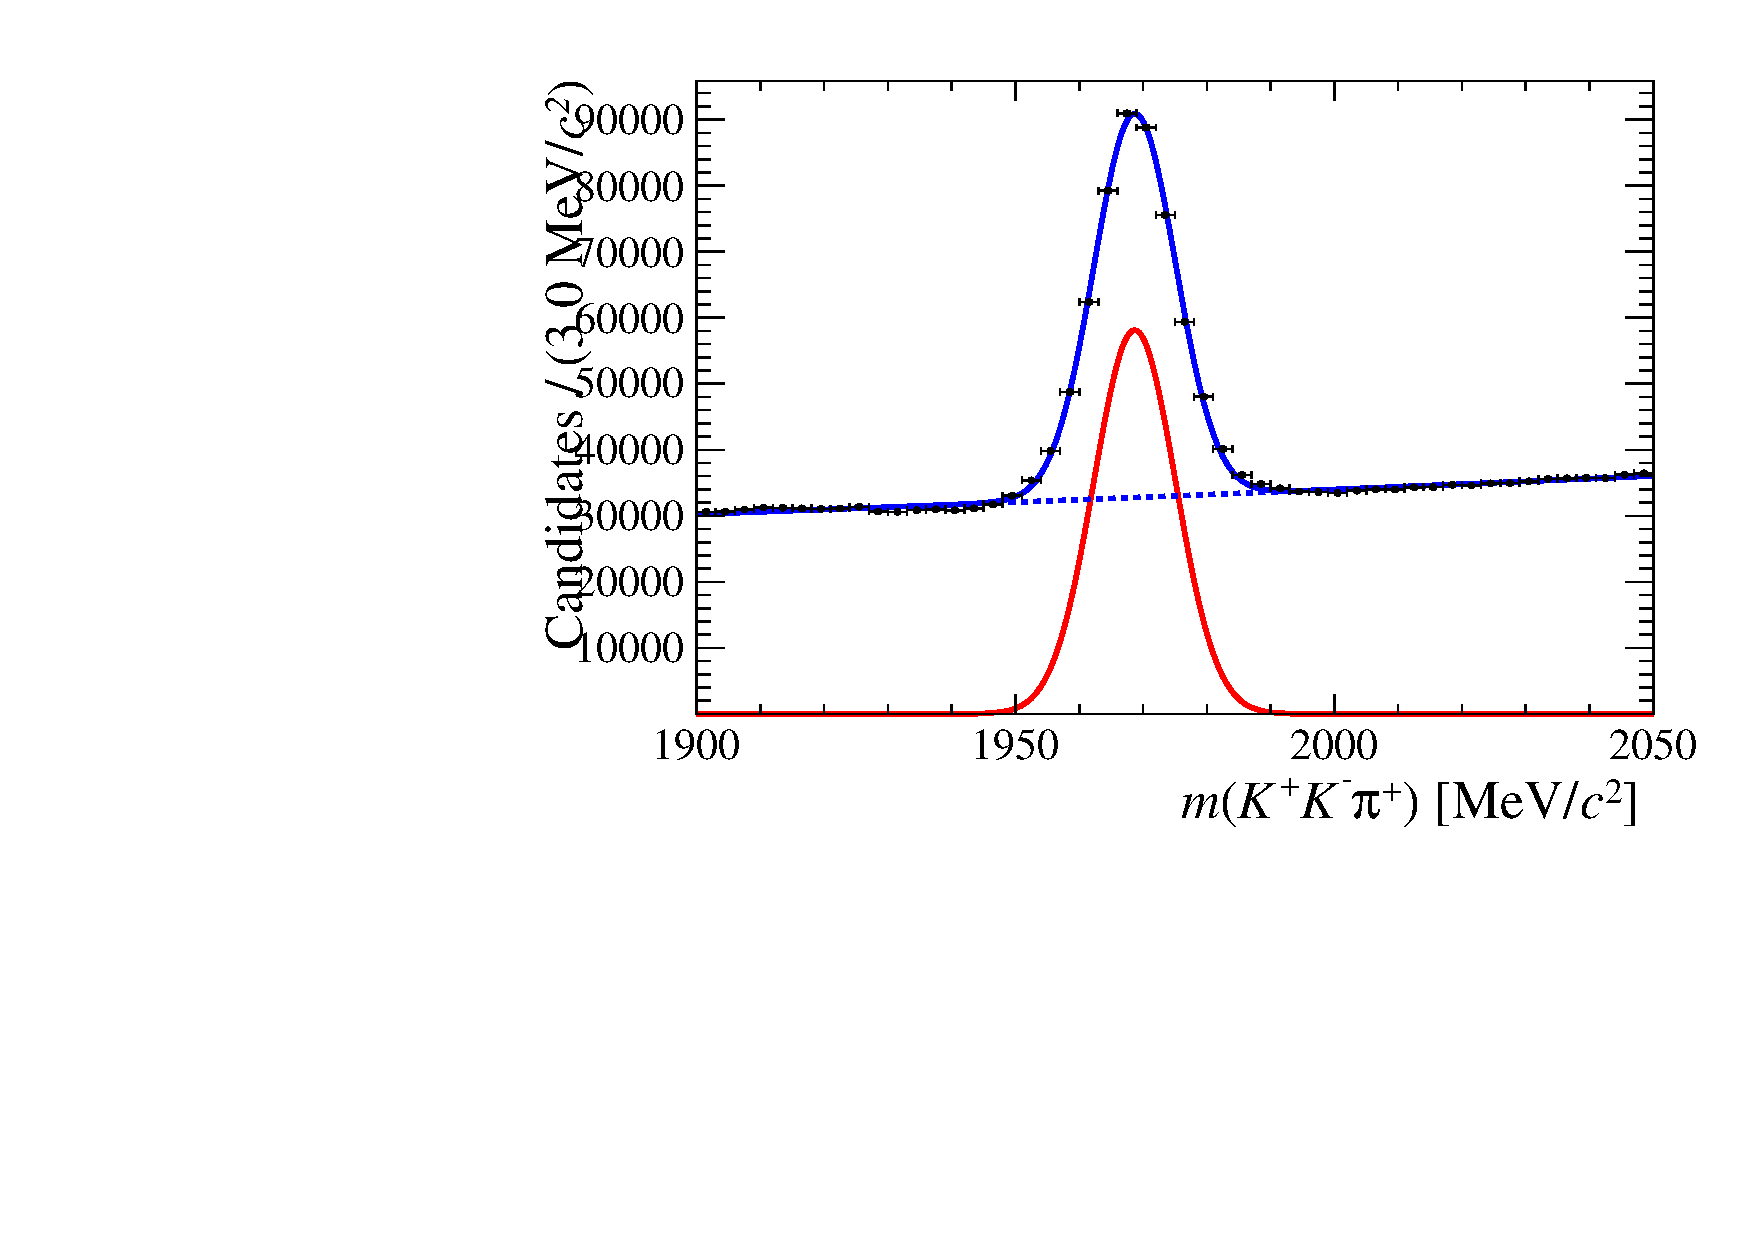
\includegraphics[width=1.0\textwidth]{figs/Selection/Fit_Data_Bs02DsPi_Ds2KKPi_2016_MagUp_PreSel.pdf}
%       \caption{\decay{\Dsp}{\Kp\Km\pip} MagUp}
%    \end{subfigure}
%    \begin{subfigure}[t]{0.4\textwidth}
%       \centering
%       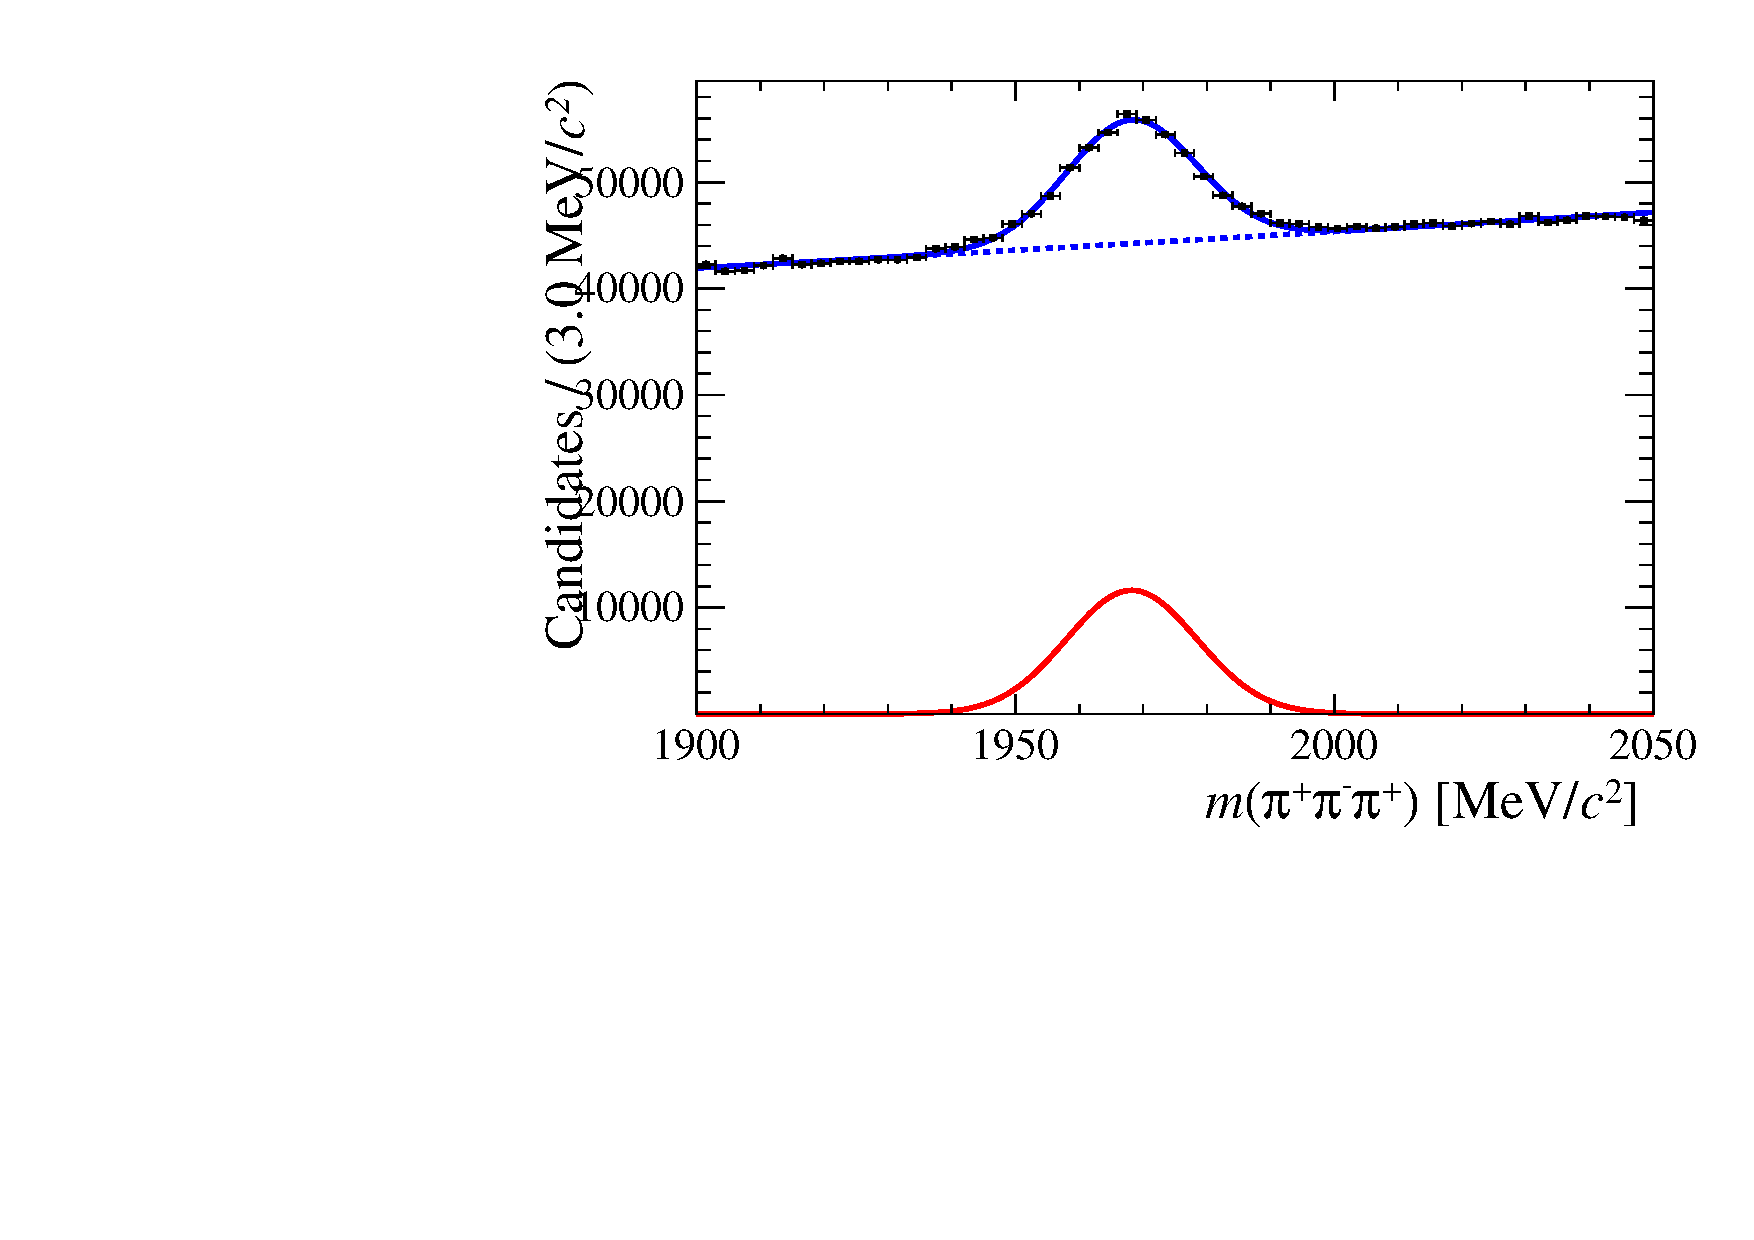
\includegraphics[width=1.0\textwidth]{figs/Selection/Fit_Data_Bs02DsPi_Ds2PiPiPi_2016_MagDown_PreSel.pdf}
%       \caption{\decay{\Dsp}{\pip\pim\pip} MagDown}
%    \end{subfigure}
%    \begin{subfigure}[t]{0.4\textwidth}
%       \centering
%       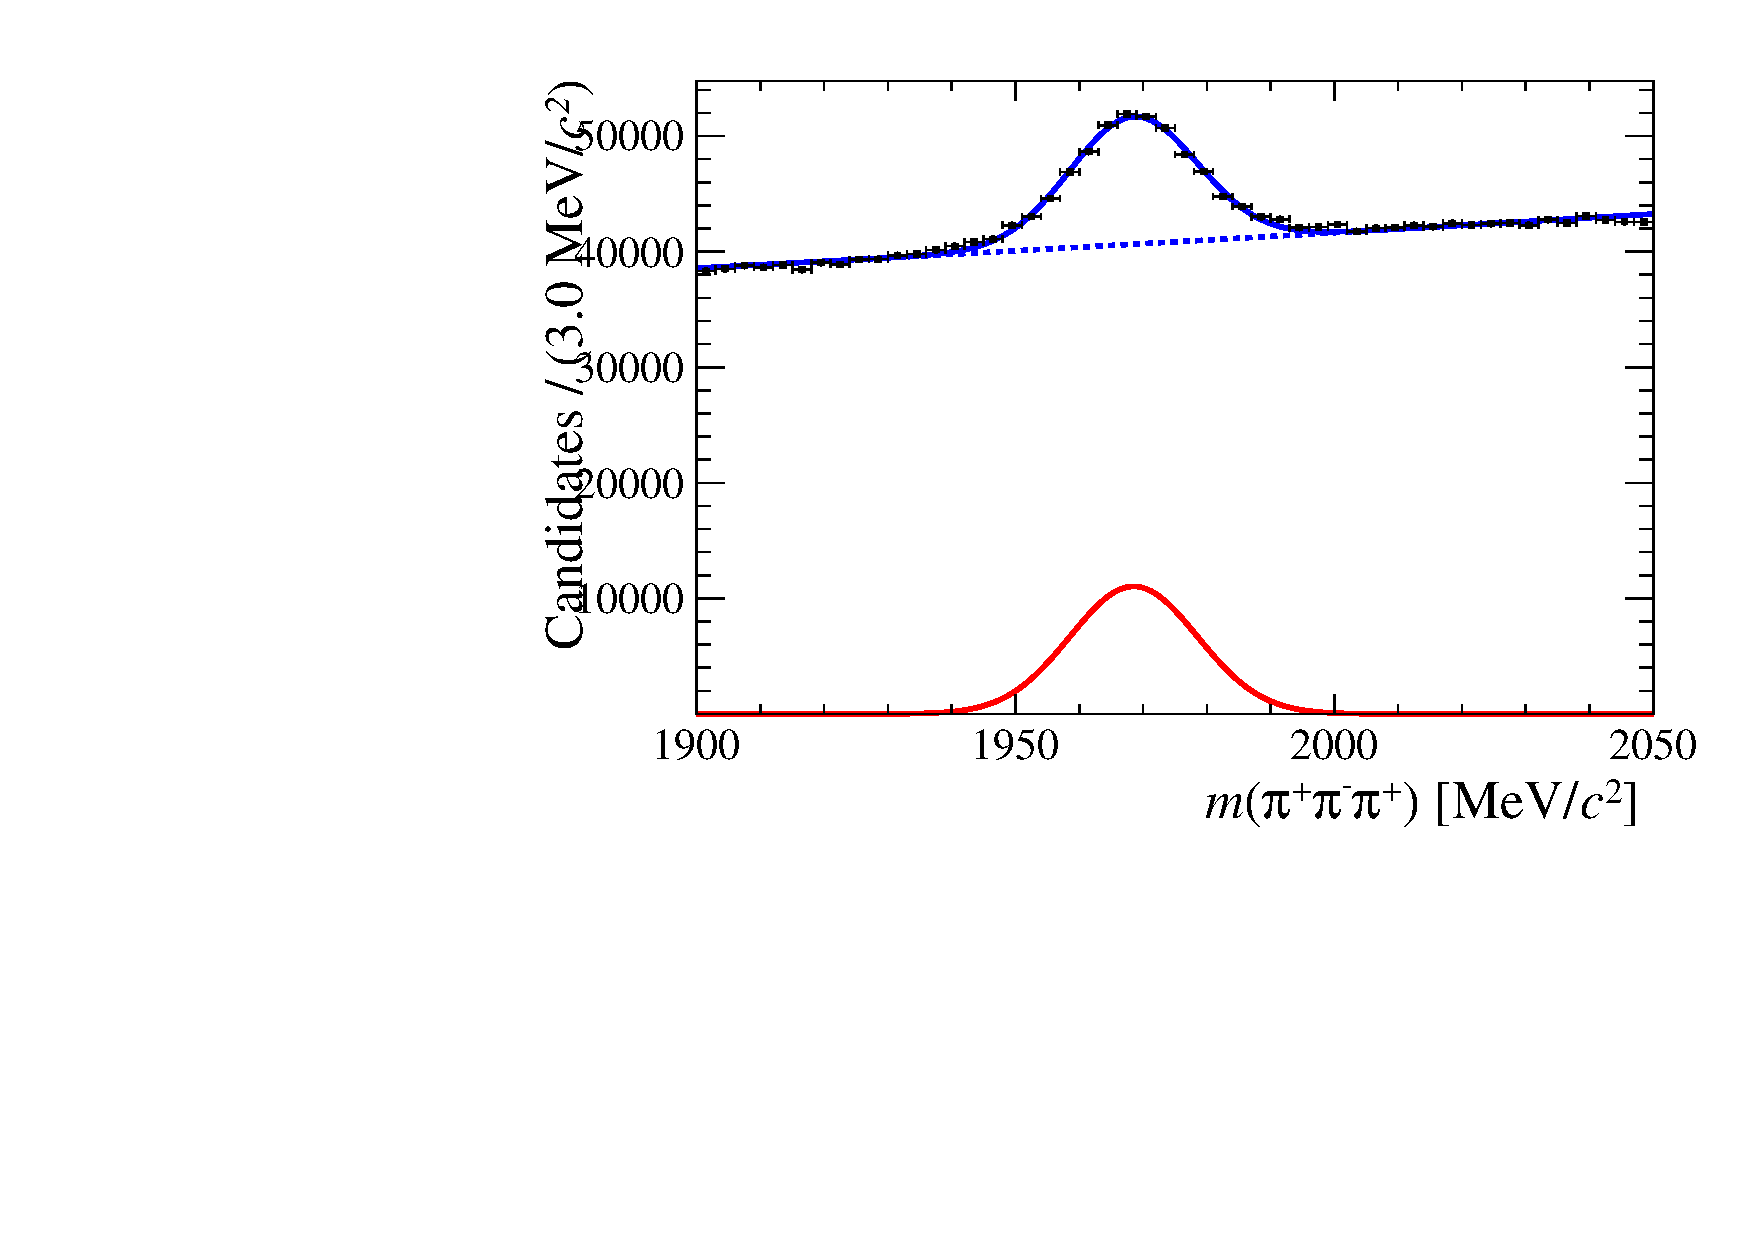
\includegraphics[width=1.0\textwidth]{figs/Selection/Fit_Data_Bs02DsPi_Ds2PiPiPi_2016_MagUp_PreSel.pdf}
%       \caption{\decay{\Dsp}{\pip\pim\pip} MagUp}
%    \end{subfigure}
%    \begin{subfigure}[t]{0.4\textwidth}
%       \centering
%       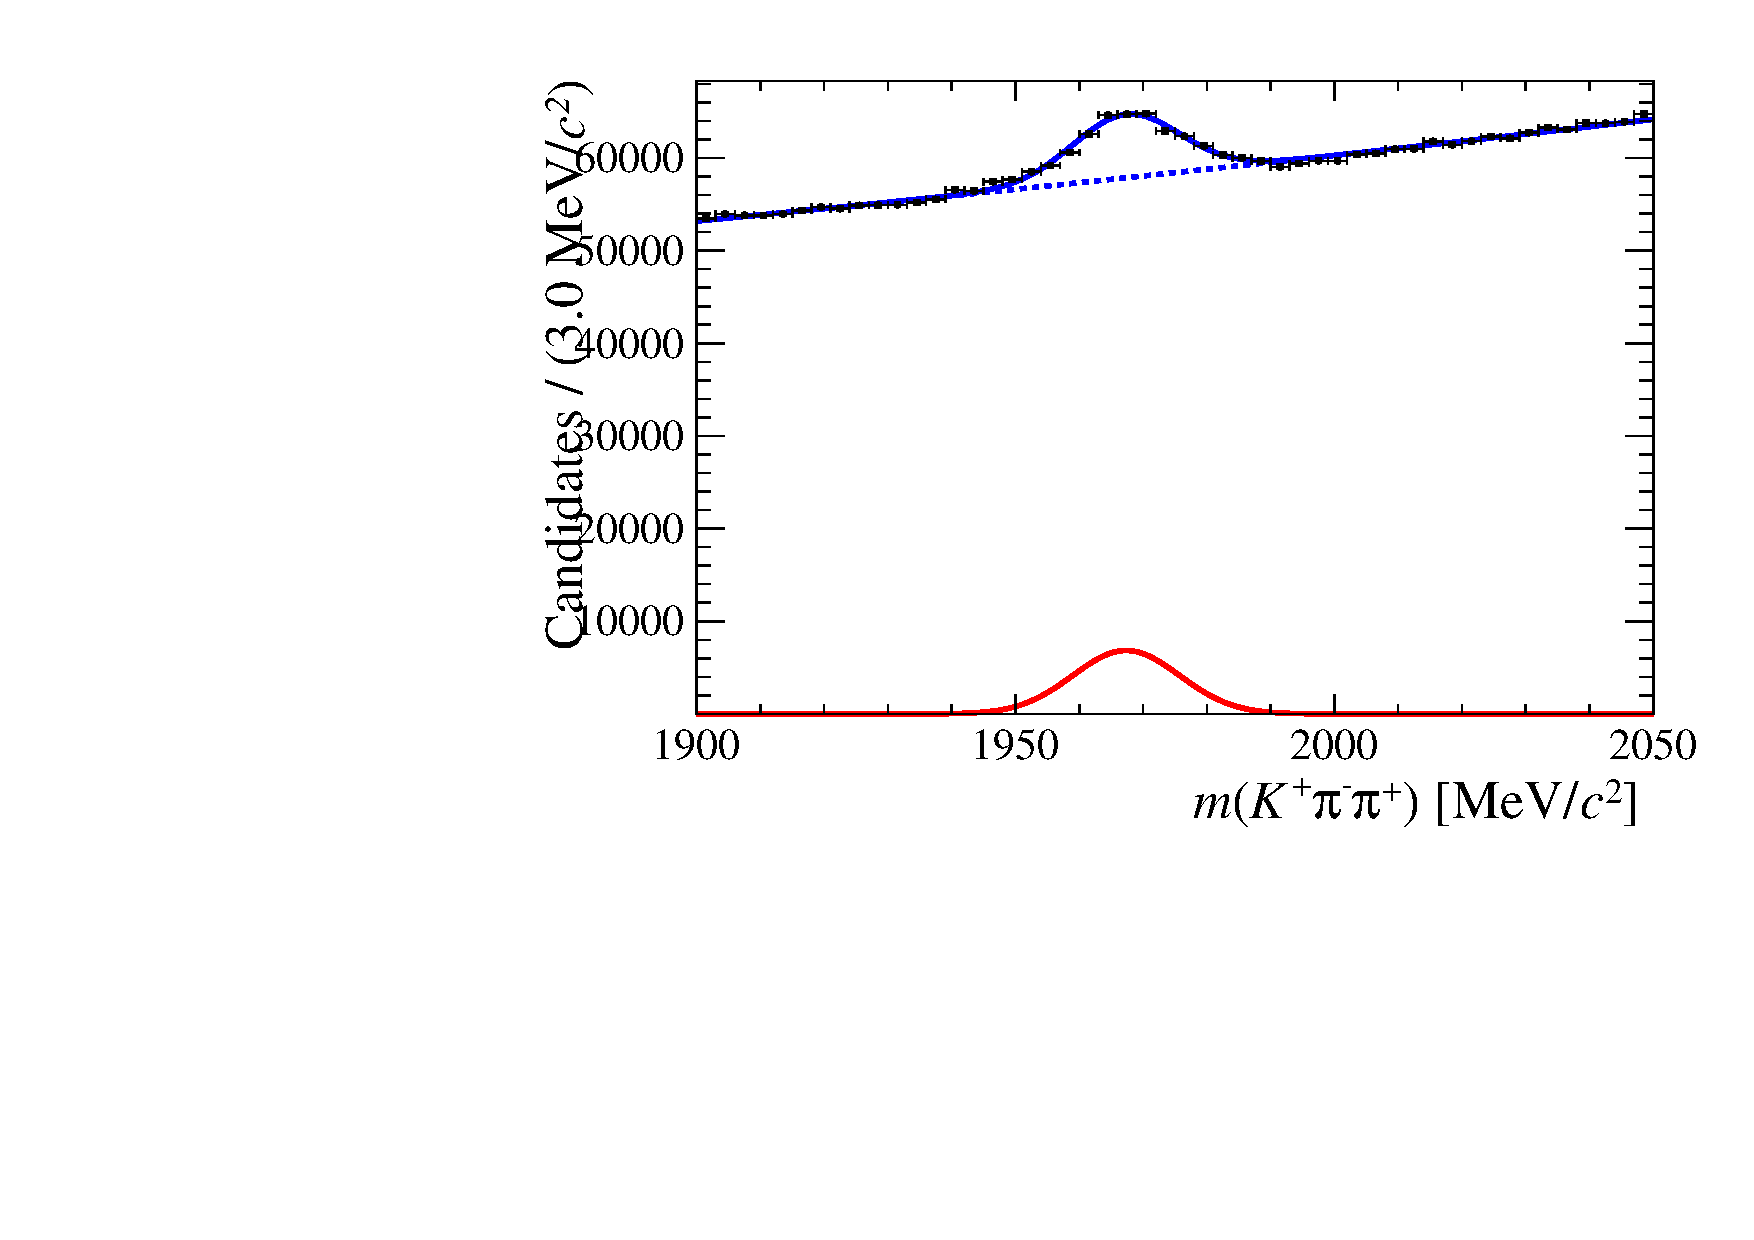
\includegraphics[width=1.0\textwidth]{figs/Selection/Fit_Data_Bs02DsPi_Ds2KPiPi_2016_MagDown_PreSel.pdf}
%       \caption{\decay{\Dsp}{\Kp\pim\pip} MagDown}
%    \end{subfigure}
%    \begin{subfigure}[t]{0.4\textwidth}
%       \centering
%       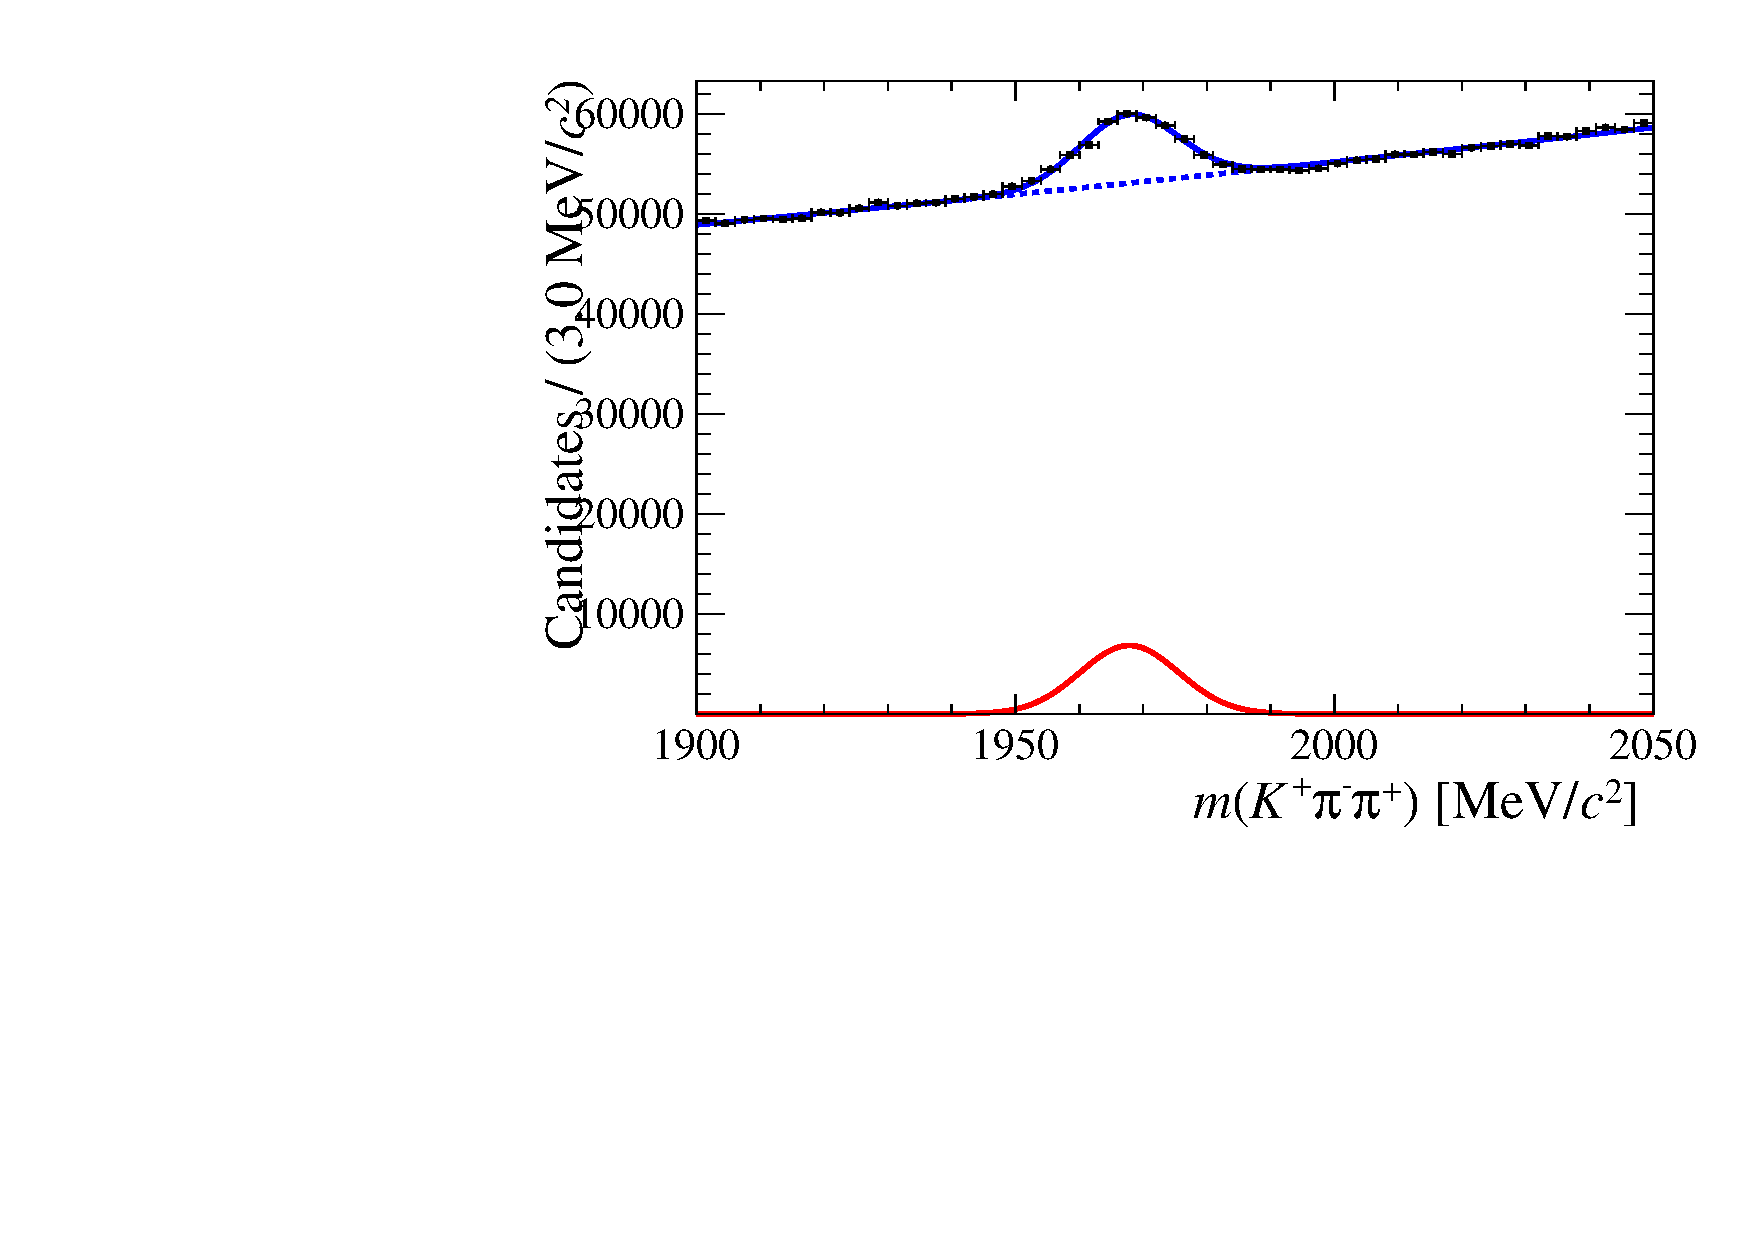
\includegraphics[width=1.0\textwidth]{figs/Selection/Fit_Data_Bs02DsPi_Ds2KPiPi_2016_MagUp_PreSel.pdf}
%       \caption{\decay{\Dsp}{\Kp\pim\pip} MagUp}
%    \end{subfigure}
%    \caption{Unbinned maximum likelihood fit to \decay{\Bs}{\jpsi\phiz} (top) and \decay{\Bsb}{\Dsp\pim} (bottom three rows) candidates. These distributions correspond to just the 2016 data samples. Slight discrepancies are observed as a result of the simplified fit model in the top two plots.}
%    \label{fig:mvatrainingsamples}
% \end{figure}


% %%%%%%%%%%%%%%%%%%%%%%%%%%%%%%%%%%%%%%%%%%%%%%%%%%%%%%%%%%
% \begin{table}[!h]
%    \centering
%       \begin{tabular}{ll S[table-format=6.0(4)] S[table-format=6.0(4)] S[table-format=7.0(4)]}
%          \hline
%          Mode                       & Year   & {MagDown}          & {MagUp}           & {Total} \\ 
%          \hline                                                
%          \decay{\phiz}{\Kp\Km}      & 2011   & 3190 \pm 170     &   2120 \pm 140  &    \\
%                                     & 2012   & 5800 \pm 200     &   5540 \pm 200  &     \\
%                                     & 2015   & 2240 \pm 110     &   1640 \pm 100  &     \\
%                                     & 2016   & 11200 \pm 300    &   11100 \pm 300 & 42830 \pm 600    \\
%          \hline                                                
%          \decay{\Dsp}{\Kp\Km\pip}   & 2011   & 97100  \pm 500   & 68600  \pm 400  &     \\
%                                     & 2012   & 216600 \pm 800   & 212800 \pm 800  &     \\
%                                     & 2015   & 68600  \pm 400   & 43400  \pm 300  &     \\
%                                     & 2016   & 321400 \pm 900   & 310800 \pm 900  & 1339300 \pm 1900    \\
%          \hline                                                
%          \decay{\Dsp}{\pip\pim\pip} & 2011   & 24300 \pm 500    &   17100 \pm 400 &      \\
%                                     & 2012   & 57700 \pm 800    &   56500 \pm 900 &     \\
%                                     & 2015   & 20400 \pm 500    &   13100 \pm 400 &     \\
%                                     & 2016   & 99200 \pm 1200   &  92100 \pm 1200 & 380400 \pm 2300    \\
%          \hline                                                
%          \decay{\Dsp}{\Kp\pim\pip}  & 2011   & 13200 \pm 600    & 9500  \pm 400   &     \\
%                                     & 2012   & 29300 \pm 900    & 29300 \pm 900   &     \\
%                                     & 2015   & 10000 \pm 500    & 6200  \pm 400   &     \\
%                                     & 2016   & 47800 \pm 1200   & 44200 \pm 1100  & 189500 \pm 2300    \\
%          \hline
%       \end{tabular}
%       \caption{Yields of the samples used to train data-driven MVAs. The total yields are summed over all years and both magnet polarities.}
%       \label{table:mva_training_yields}
   
% \end{table}
% %%%%%%%%%%%%%%%%%%%%%%%%%%%%%%%%%%%%%%%%%%%%%%%%%%%%%%%%%%

\subsubsection{Input variables}


%% Discussion of input variables
The MVA method is trained using a large set of variables chosen to help discriminate between the signals of interest and combinations of unrelated tracks. These variables include the properties of the \Kpm or \pipm decay products as well as those of the \phiz or \Dsp candidate itself. Many of the quantities are the same as those previously defined in Section.~\ref{sec:selectionrequirements}. The additional parameters relate to the track quality and particle identification information and are defined as follows:

\begin{description}
\item \textbf{Track matching quality, $\chi^{2}_{\text{TRKMATCH}}$}: this parameter is an key component of the pattern recognition software that matches the \velo and tracking station track sections together to form \emph{long} tracks. It quantifies the quality of the track matching; incorrect combinations of track sections can have larger $\chi^{2}_{\text{TRKMATCH}}$ values than true tracks.  

\item \textbf{\velo track quality, $\chi^{2}_{\text{TRKVELO}}$}: this quantifies the quality of the track fit using just the hits in the \velo. Incorrect combinations of hits are likely to have higher values of $\chi^{2}_{\text{TRKVELO}}$ than true tracks.  


\item \textbf{Kaon, proton, pion and ghost probabilities, ProbNN$x$ ($x\in[K,\pi,\proton,\text{ghost}]$)}: these variables are an alternative form of \emph{Particle Identification} variables in addition to those already discussed in Section~\ref{sec:pidrequirements}. Each ProbNN$x$ variable acts as the probability for the reconstructed track to be of the species $x$. These variables are the responses of Artificial Neural Networks trained to differentiate between the various particle types using a large number of inputs from different sub-detectors. The trainings use simulated samples of signal and background decays and have been retuned between Run~I and Run~II to reflect the difference in the detector configuration. These variables improve the performance over the variables discussed in Section~\ref{sec:pidrequirements} by using input from all PID sub-detectors and exploiting any correlations.   
 Four of the available ProbNN$x$ variables are used in this analysis. Three of these identify kaons, protons and pions. The last aims to identify ghost tracks, similar to the $P_{\text{Ghost}}$ variable already discussed. 
\end{description}

The variables used in the \phiz and \Dsp meson MVAs are listed in Table~\ref{tab:mvavars}. 
%Some of the variables are input into the MVA training algorithm as their logarithm, rather than the variable directly. These variables tend to be rapidly increasing in at certain values, so using the logarithm aids visualisation. 
A total of 24 and 35 variables are used in the \phiz and \Dsp MVAs respectively.

When training the \phiz meson MVA, the flight distance significance is not included as an input variable. This MVA is used to select both \phiz and \Dzb mesons which are likely to have different flight distance significance distributions as a result of their different lifetimes. 
%The \Dsp MVA includes the flight distance significance as these mesons decay displaced from their production vertex.


\begin{table}[h]
   \centering
      \begin{tabular}{ l l l c c}

         \hline
         Particle       & Description                    & Quantity                             & \Dsp MVA      & \phiz MVA    \\    
         \hline
         \phiz/\Dsp     & Momentum                       &  \ptot                               & \checkmark    & \checkmark   \\  
                        & Transverse Momentum            &  \pt                                 & \checkmark    & \checkmark   \\  
                        & Vertex quality                 &  $\log_{10}(\chi^{2}_{\text{VXT}})$  & \checkmark    & \checkmark   \\  
                        & Impact parameter significance  &  $\log_{10}(\chi^{2}_{\text{IP}})$   & \checkmark    & \checkmark   \\    
                        & Flight distance significance   &  $\log_{10}(\chi^{2}_{\text{FD}})$   & \checkmark    & -            \\    
         \hline
         \Kpm           & Momentum                       &  \ptot                               & \checkmark    & \checkmark   \\  
                        & Transverse momentum            &  \pt                                 & \checkmark    & \checkmark   \\ 
                        & Longitudinal momentum          &  \pz                                 & \checkmark    & -            \\
                        & Impact parameter significance  &  $\log_{10}(\chi^{2}_{\text{IP}})$   & \checkmark    & \checkmark   \\    
                        & Track quality                  &  $\chi^{2}_{\text{TRK}}$             & \checkmark    & \checkmark   \\    
                        & Velo track quality             &  $\chi^{2}_{\text{TRKVELO}}$         & \checkmark    & -            \\    
                        & Track matching quality         &  $\chi^{2}_{\text{TRKMATCH}}$        & \checkmark    & \checkmark   \\    
                        & Kaon probability               &  ProbNNk                             & \checkmark    & \checkmark   \\    
                        & Proton probability             &  ProbNNp                             & \checkmark    & \checkmark   \\    
                        & Pion probability               &  ProbNNpi                            & \checkmark    & \checkmark   \\    
                        & Ghost probability              &  ProbNNghost                         & \checkmark    & \checkmark   \\    
         \hline
      \end{tabular}
   
   \caption{Discriminating variables used to train the \phiz and \Dsp MVAs. Poorly discriminating variables are removed from the \phiz MVA to prevent overtraining. The flight distance significance is remove as the MVA is applied to both \phiz and \Dzb candidates.}
   \label{tab:mvavars}
\end{table}
 
%The variables used in the \Dsp MVA are also listed in Table~\ref{tab:mvavars}. 
%These are largely very similar to those used for the \phiz meson MVA, however it also includes the \Dsp meson's flight distance significance as, unlike the \phiz meson, the \Dsp meson decays displaced from its production vertex. 
%A total of 35 variables are used in these MVAs.



% \begin{table}[h]
%    \centering
%       \begin{tabular}{ l l l}

%          \hline
%          Particle       & Description                    & Quantity                          \\    
%          \hline
%          \Dsp           & Momentum                       &  \ptot                            \\  
%                         & Transverse Momentum            &  \pt                              \\  
%                         & Vertex quality                 &  $\log_{10}(\chi^{2}_{\text{VXT}})$    \\  
%                         & Impact parameter significance  &  $\log_{10}(\chi^{2}_{\text{IP}})$     \\    
%                         & Flight distance significance   &  $\log_{10}(\chi^{2}_{\text{FD}})$     \\    
%          \hline
%          \Kpm, \pipm    & Momentum                       &  \ptot                            \\  
%                         & Transverse momentum            &  \pt                              \\
%                         & Impact parameter significance  &  $\log_{10}(\chi^{2}_{\text{IP}})$     \\    
%                         & Track quality                  &  $\chi^{2}_{\text{TRK}}$          \\    
%                         & Velo track quality             &  $\chi^{2}_{\text{TRKVELO}}$      \\    
%                         & Track matching quality         &  $\chi^{2}_{\text{TRKMATCH}}$     \\    
%                         & Kaon probability               &  ProbNNk                          \\    
%                         & Proton probability             &  ProbNNp                          \\    
%                         & Pion probability               &  ProbNNpi                         \\    
%                         & Ghost probability              &  ProbNNghost                      \\    
%          \hline
%       \end{tabular}
   
%    \caption{Discriminating variables used to train the \Dsp MVAs.}
%    \label{tab:mvavars_ds}
% \end{table}


When training the MVA methods, the variables are ranked according to their discrimination power. 
It is found that the kaon particle identification variable and various $\log_{10}(\chi^{2}_{\text{IP}})$ variables are the most discriminating as detailed in Appendix~\ref{sec:App_MVA_input}.
%Examples of these ranking are shown for the Run~II, \decay{\phiz}{\Kp\Km} MVA and Run~II, \decay{\Dsp}{\Kp\Km\pip} MVA in Table~\ref{tab:mvarank_dsandphi}. 
%It can be seen that for both the \Dsp and \phiz meson MVAs that the kaon particle identification variable and various $\log_{10}(\chi^{2}_{\text{IP}})$ variables are the most discriminating.

% \begin{table}[h]
% \centering
% \scalebox{1.0}{
% \begin{tabular}{ c l c | c l c}

% \hline 

% \multicolumn{3}{c|}{\decay{\Dsp}{\Kp\Km\pip}}                 & \multicolumn{3}{c}{\decay{\phiz}{\Kp\Km}}                       \\
% Rank & Variable                             & Importance (\%) & Rank & Variable                           & Importance (\%)      \\
% \hline
%  1 & \Kp ProbNNk                            & $7.6$ &  1 & \Kp ProbNNk                                & $6.0$\\
%  2 & \Km ProbNNk                            & $6.0$ &  2 & \phiz $\log_{10}(\chi^{2}_{\text{IP}})$    & $6.0$\\
%  3 & \Kp $\log_{10}(\chi^{2}_{\text{IP}})$  & $5.5$ &  3 & \Km $\log_{10}(\chi^{2}_{\text{IP}})$      & $6.0$\\
%  4 & \pip $\log_{10}(\chi^{2}_{\text{IP}})$ & $5.0$ &  4 & \phiz $\log_{10}(\chi^{2}_{\text{VTX}})$   & $5.8$\\
%  5 & \Kp \ptot                              & $4.3$ &  5 & \Km ProbNNpi                               & $5.8$\\
%  6 & \Dsp $\log_{10}(\chi^{2}_{\text{IP}})$ & $4.1$ &  6 & \Kp $\log_{10}(\chi^{2}_{\text{IP}})$      & $5.8$\\
%  7 & \pip \pt                               & $4.0$ &  7 & \Kp ProbNNghost                            & $5.4$\\
%  8 & \Kp \pt                                & $3.9$ &  8 & \Km ProbNNk                                & $5.4$\\
%  9 & \pip ProbNNpi                          & $3.9$ &  9 & \Kp $\chi^{2}_{\text{TRK}}$                & $5.6$\\
% 10 & \Dsp $\log_{10}(\chi^{2}_{\text{FD}})$ & $3.8$ & 10 & \Km $\chi^{2}_{\text{TRK}}$                & $5.2$\\
% 11 & \Km $\log_{10}(\chi^{2}_{\text{IP}})$  & $3.7$ & 11 & \Kp ProbNNpi                               & $5.2$\\
% 12 & \Dsp $\log_{10}(\chi^{2}_{\text{VTX}})$& $3.0$ & 12 & \Km ProbNNghost                            & $5.0$\\
% 13 & \Km \ptot                              & $2.8$ & 13 & \Kp ProbNNp                                & $4.5$\\
% 14 & \Kp ProbNNp                            & $2.8$ & 14 & \Km ProbNNp                                & $4.4$\\
% 15 & \Km ProbNNp                            & $2.7$ & 15 & \Kp $\chi^{2}_{\text{TRKMATCH}}$           & $4.3$\\
% % 16 & \pip ProbNNghost                   & $2.623$ & 16 & \Km $\chi^{2}_{\text{TRKMATCH}}$     & $3.977\times 10^{-2}$\\
% % 17 & \Kp ProbNNghost                    & $2.593$ & 17 & \Km \pt                              & $3.437\times 10^{-2}$\\
% % 18 & \Dsp \pt                           & $2.543$ & 18 & \Kp \pt                              & $3.012\times 10^{-2}$\\
% % 19 & \Kp ProbNNpi                       & $2.525$ & 19 & \phiz PT                             & $2.400\times 10^{-2}$\\
% % 20 & \Km \pt                            & $2.355$ & 20 & \phiz P                              & $1.792\times 10^{-2}$\\
% % 21 & \Dsp \ptot                         & $2.327$ & 21 & \Km \pz                              & $1.397\times 10^{-2}$\\
% % 22 & \Km ProbNNpi                       & $2.226$ & 22 & \Km \ptot                            & $1.387\times 10^{-2}$\\
% % 23 & \pip \ptot                         & $2.083$ & 23 & \Kp \pz                              & $1.245\times 10^{-2}$\\
% % 24 & \pip ProbNNp                       & $1.849$ & 24 & \Kp \ptot                            & $1.218\times 10^{-2}$\\
% % 25 & \pip ProbNNk                       & $1.793$ \\
% % 26 & \Km ProbNNghost                    & $1.607$ \\
% % 27 & \pip $\chi^{2}_{\text{TRKVELO}}$   & $1.589$ \\
% % 28 & \Km $\chi^{2}_{\text{TRK}}$        & $1.588$ \\
% % 29 & \pip $\chi^{2}_{\text{TRKMATCH}}$  & $1.548$ \\
% % 30 & \Kp $\chi^{2}_{\text{TRK}}$        & $1.522$ \\
% % 31 & \Km $\chi^{2}_{\text{TRKMATCH}}$   & $1.442$ \\
% % 32 & \pip $\chi^{2}_{\text{TRK}}$       & $1.433$ \\
% % 33 & \Kp $\chi^{2}_{\text{TRKVELO}}$    & $1.184$ \\
% % 34 & \Kp $\chi^{2}_{\text{TRKMATCH}}$   & $1.176$ \\
% % 35 & \Km $\chi^{2}_{\text{TRKVELO}}$    & $8.818\times10^{-3}$ \\
% \hline
% \end{tabular}
% }
% \caption{Ranking of variables for the 15 highest ranked variables used to train the \decay{\Dsp}{\Kp\Km\pip} (left) and \decay{\phiz}{\Kp\Km} (right) Run~II MVAs.}
% \label{tab:mvarank_dsandphi}
% \end{table}


% %%%%%%%%%%%%%%%%%%%%%%%%%%%%%%%%%%%%%%%%%%%%%%%%%%%%%%%%%%
% \begin{figure}[!h]
%    \centering
%    \begin{subfigure}[t]{0.22\textwidth}
%       \centering
%       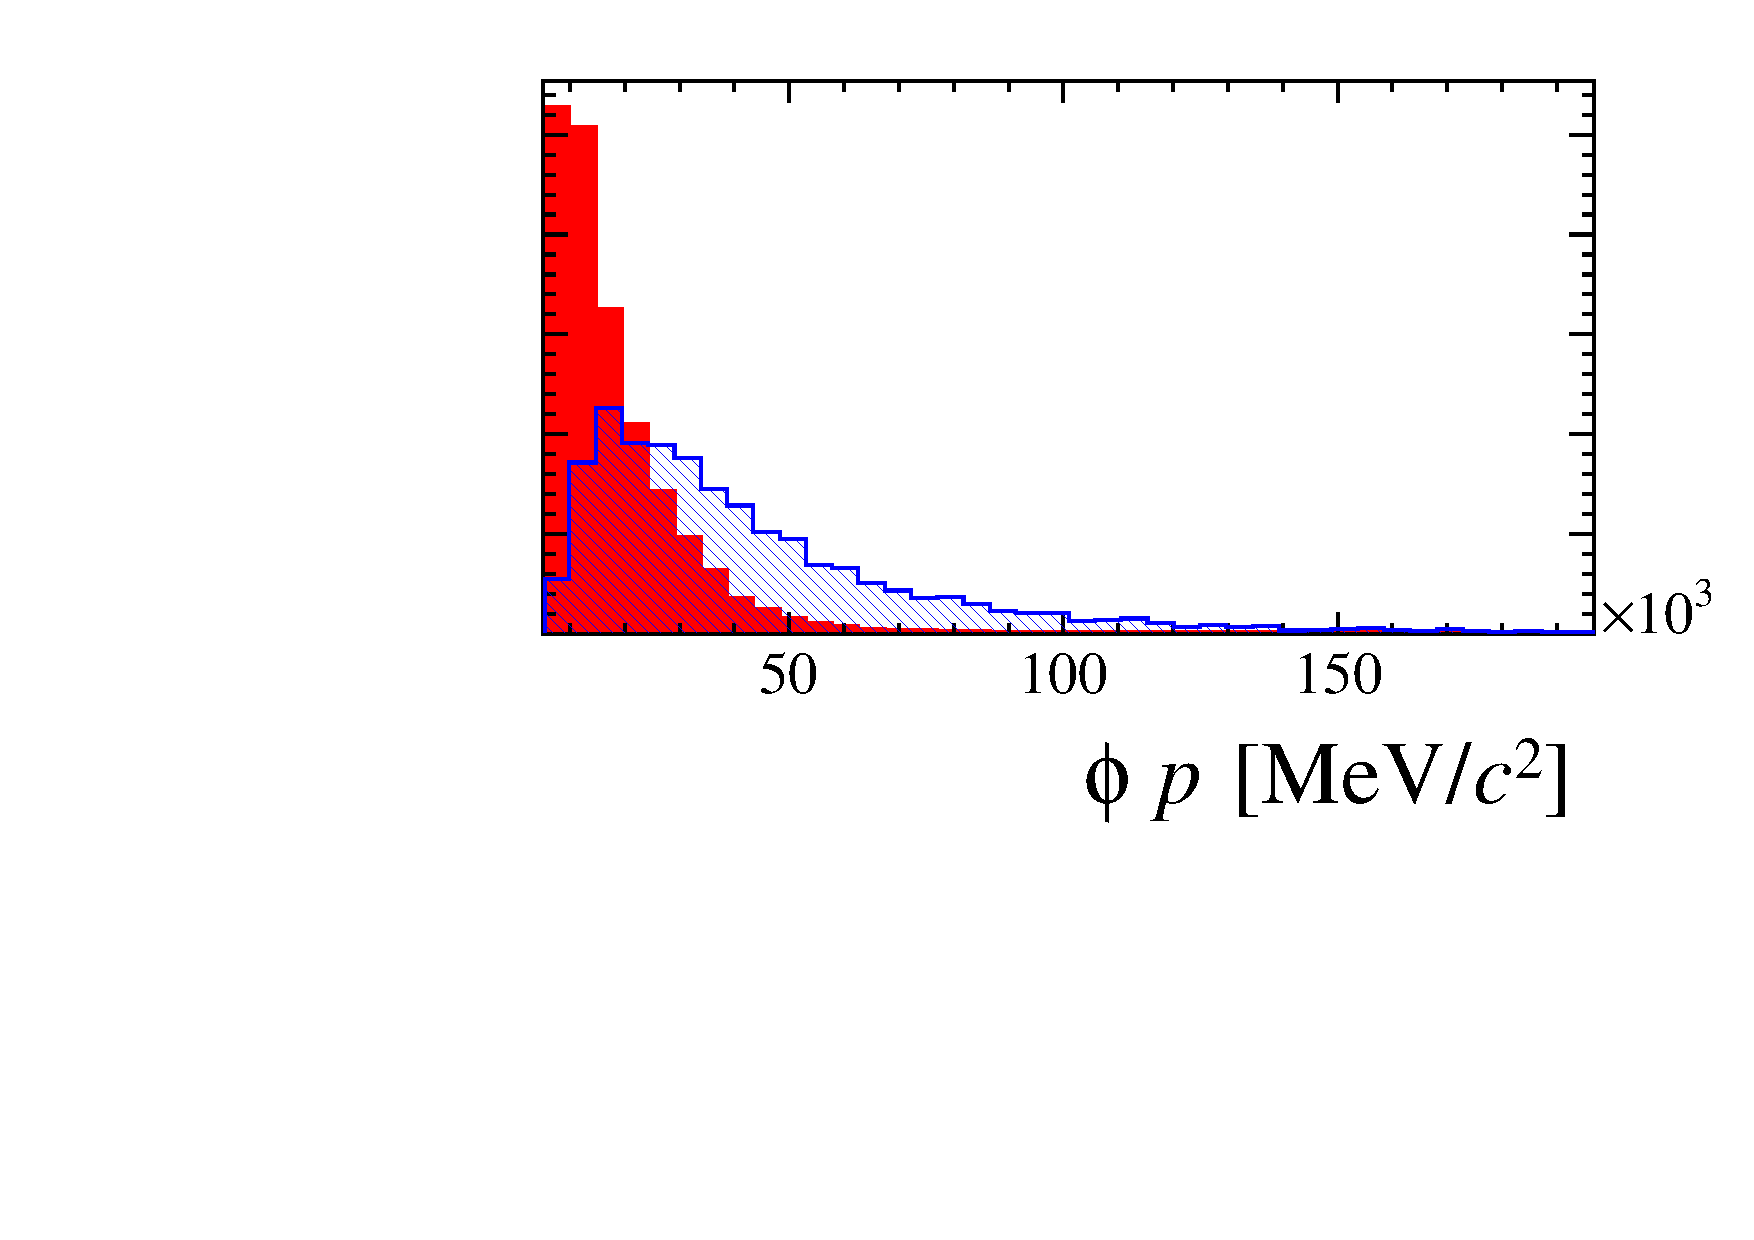
\includegraphics[width=1.0\textwidth]{figs/Selection/Phi_BDT_Var_Ds2KKPi_Phi_P.pdf}
%    \end{subfigure}
%    \begin{subfigure}[t]{0.22\textwidth}
%       \centering
%       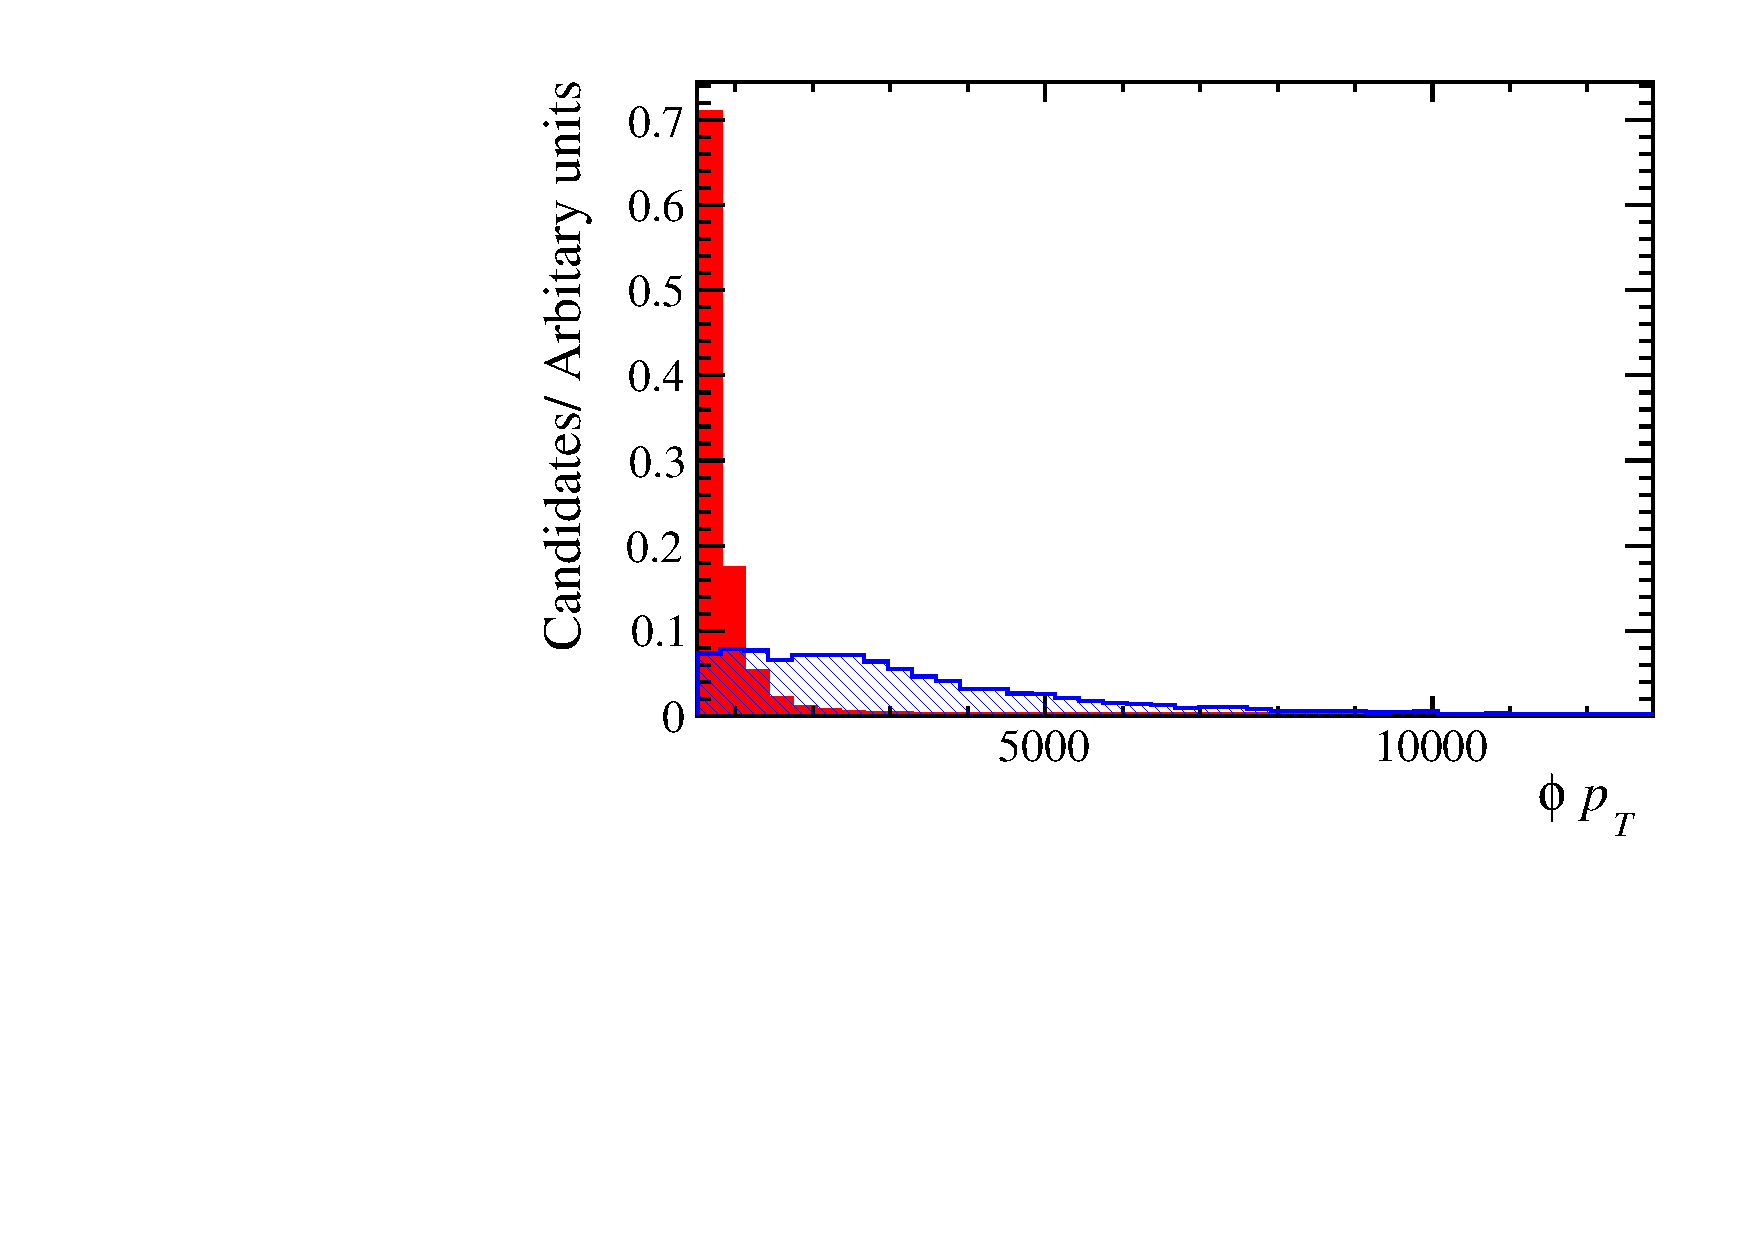
\includegraphics[width=1.0\textwidth]{figs/Selection/Phi_BDT_Var_Ds2KKPi_Phi_PT.pdf}
%    \end{subfigure}
%    \begin{subfigure}[t]{0.22\textwidth}
%       \centering
%       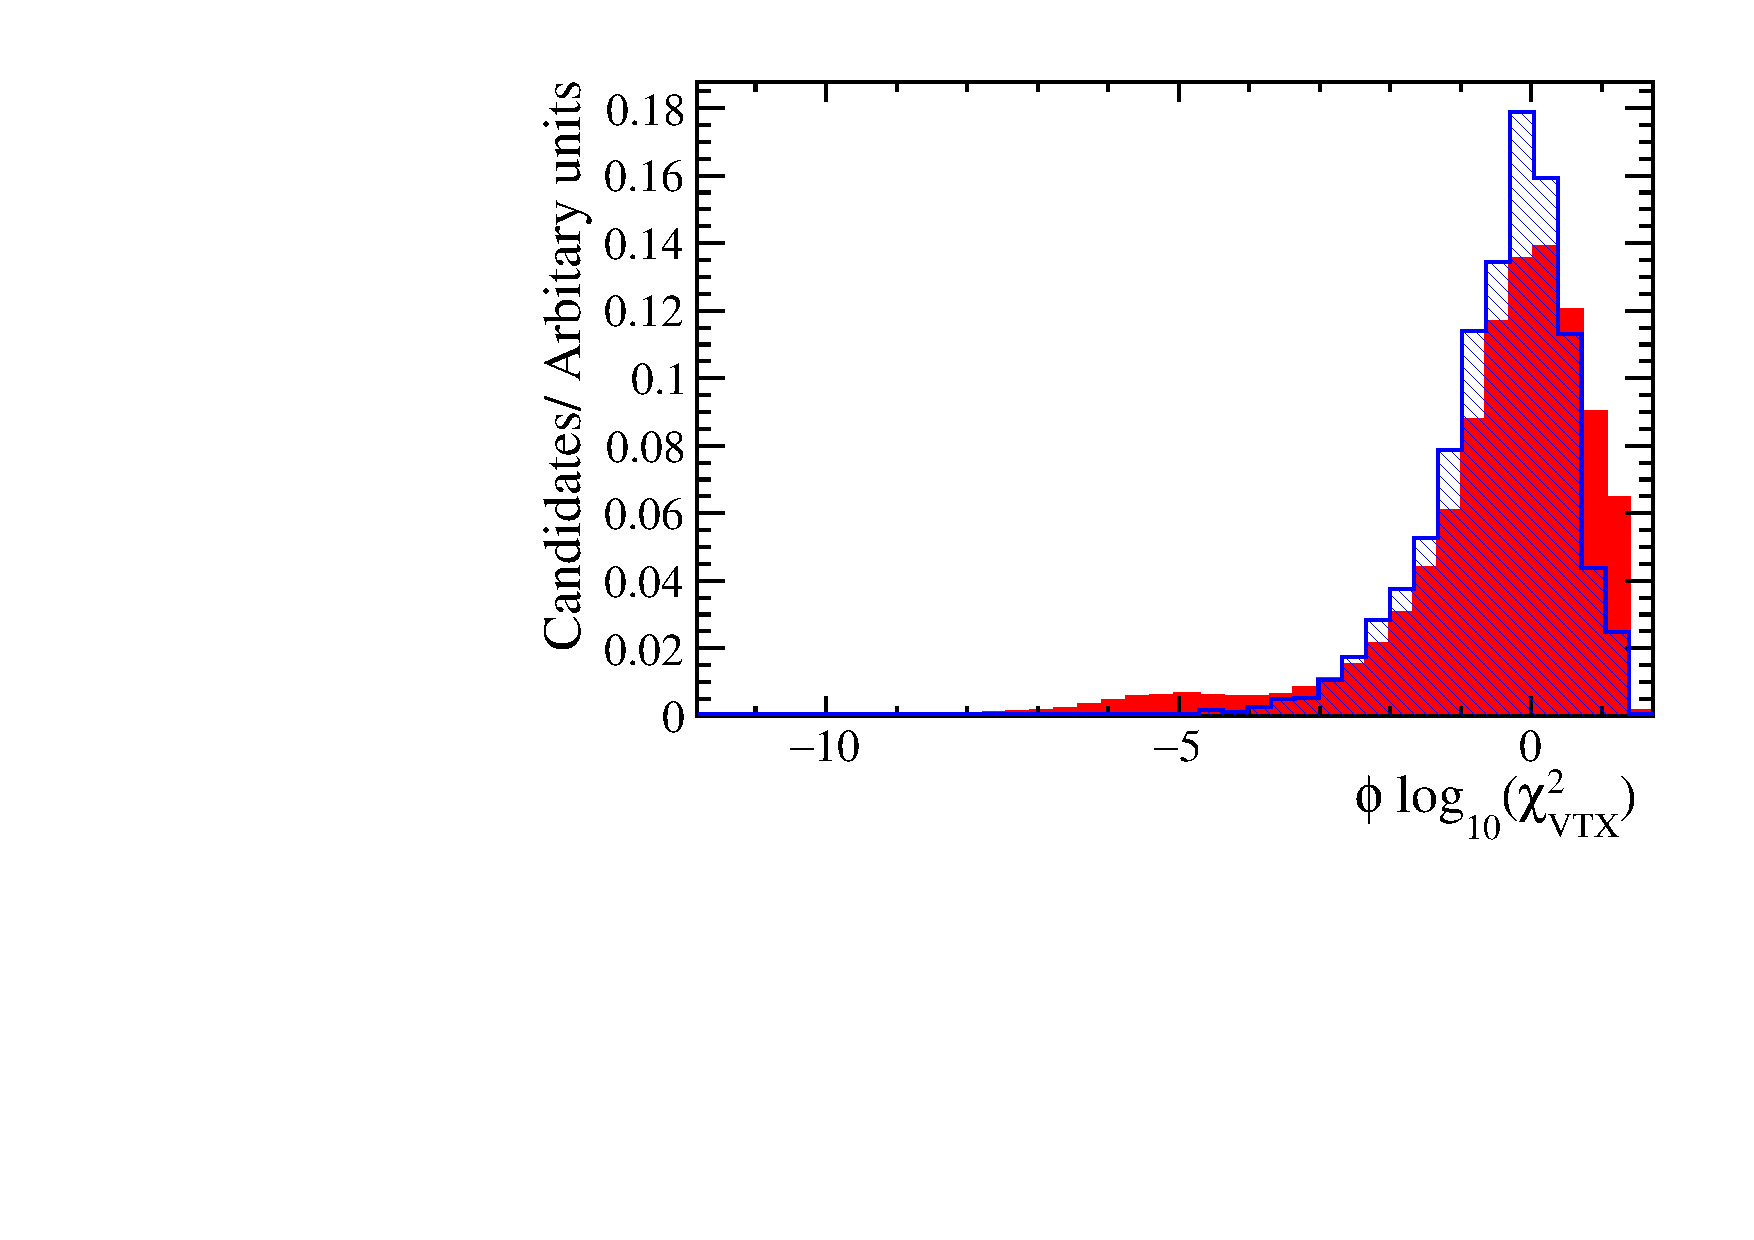
\includegraphics[width=1.0\textwidth]{figs/Selection/Phi_BDT_Var_Ds2KKPi_log10_Phi_ENDVERTEX_CHI2.pdf}
%    \end{subfigure}
%    \begin{subfigure}[t]{0.22\textwidth}
%       \centering
%       \includegraphics[width=1.0\textwidth]{figs/Selection/Phi_BDT_Var_Ds2KKPi_log10_Phi_IPCHI2_OWNPV.pdf}
%    \end{subfigure}
%    \begin{subfigure}[t]{0.22\textwidth}
%       \centering
%       \includegraphics[width=1.0\textwidth]{figs/Selection/Phi_BDT_Var_Ds2KKPi_Phi_K0_P.pdf}
%    \end{subfigure}
%    \begin{subfigure}[t]{0.22\textwidth}
%       \centering
%       \includegraphics[width=1.0\textwidth]{figs/Selection/Phi_BDT_Var_Ds2KKPi_Phi_K1_P.pdf}
%    \end{subfigure}
%    \begin{subfigure}[t]{0.22\textwidth}
%       \centering
%       \includegraphics[width=1.0\textwidth]{figs/Selection/Phi_BDT_Var_Ds2KKPi_Phi_K0_PT.pdf}
%    \end{subfigure}
%    \begin{subfigure}[t]{0.22\textwidth}
%       \centering
%       \includegraphics[width=1.0\textwidth]{figs/Selection/Phi_BDT_Var_Ds2KKPi_Phi_K1_PT.pdf}
%    \end{subfigure}
%    \begin{subfigure}[t]{0.22\textwidth}
%       \centering
%       \includegraphics[width=1.0\textwidth]{figs/Selection/Phi_BDT_Var_Ds2KKPi_Phi_K0_PZ.pdf}
%    \end{subfigure}
%    \begin{subfigure}[t]{0.22\textwidth}
%       \centering
%       \includegraphics[width=1.0\textwidth]{figs/Selection/Phi_BDT_Var_Ds2KKPi_Phi_K1_PZ.pdf}
%    \end{subfigure}
%    \begin{subfigure}[t]{0.22\textwidth}
%       \centering
%       \includegraphics[width=1.0\textwidth]{figs/Selection/Phi_BDT_Var_Ds2KKPi_log10_Phi_K0_IPCHI2_OWNPV.pdf}
%    \end{subfigure}
%    \begin{subfigure}[t]{0.22\textwidth}
%       \centering
%       \includegraphics[width=1.0\textwidth]{figs/Selection/Phi_BDT_Var_Ds2KKPi_log10_Phi_K1_IPCHI2_OWNPV.pdf}
%    \end{subfigure}
%    \begin{subfigure}[t]{0.22\textwidth}
%       \centering
%       \includegraphics[width=1.0\textwidth]{figs/Selection/Phi_BDT_Var_Ds2KKPi_Phi_K0_MC15TuneV1_ProbNNk.pdf}
%    \end{subfigure}
%    \begin{subfigure}[t]{0.22\textwidth}
%       \centering
%       \includegraphics[width=1.0\textwidth]{figs/Selection/Phi_BDT_Var_Ds2KKPi_Phi_K1_MC15TuneV1_ProbNNk.pdf}
%    \end{subfigure}
%    \begin{subfigure}[t]{0.22\textwidth}
%       \centering
%       \includegraphics[width=1.0\textwidth]{figs/Selection/Phi_BDT_Var_Ds2KKPi_Phi_K0_MC15TuneV1_ProbNNp.pdf}
%    \end{subfigure}
%    \begin{subfigure}[t]{0.22\textwidth}
%       \centering
%       \includegraphics[width=1.0\textwidth]{figs/Selection/Phi_BDT_Var_Ds2KKPi_Phi_K1_MC15TuneV1_ProbNNp.pdf}
%    \end{subfigure}
%    \begin{subfigure}[t]{0.22\textwidth}
%       \centering
%       \includegraphics[width=1.0\textwidth]{figs/Selection/Phi_BDT_Var_Ds2KKPi_Phi_K0_MC15TuneV1_ProbNNpi.pdf}
%    \end{subfigure}
%    \begin{subfigure}[t]{0.22\textwidth}
%       \centering
%       \includegraphics[width=1.0\textwidth]{figs/Selection/Phi_BDT_Var_Ds2KKPi_Phi_K1_MC15TuneV1_ProbNNpi.pdf}
%    \end{subfigure}
%    \begin{subfigure}[t]{0.22\textwidth}
%       \centering
%       \includegraphics[width=1.0\textwidth]{figs/Selection/Phi_BDT_Var_Ds2KKPi_Phi_K0_MC15TuneV1_ProbNNghost.pdf}
%    \end{subfigure}
%    \begin{subfigure}[t]{0.22\textwidth}
%       \centering
%       \includegraphics[width=1.0\textwidth]{figs/Selection/Phi_BDT_Var_Ds2KKPi_Phi_K1_MC15TuneV1_ProbNNghost.pdf}
%    \end{subfigure}
%    \begin{subfigure}[t]{0.22\textwidth}
%       \centering
%       \includegraphics[width=1.0\textwidth]{figs/Selection/Phi_BDT_Var_Ds2KKPi_Phi_K0_TRACK_CHI2NDOF.pdf}
%    \end{subfigure}
%    \begin{subfigure}[t]{0.22\textwidth}
%       \centering
%       \includegraphics[width=1.0\textwidth]{figs/Selection/Phi_BDT_Var_Ds2KKPi_Phi_K1_TRACK_CHI2NDOF.pdf}
%    \end{subfigure}
%    \begin{subfigure}[t]{0.22\textwidth}
%       \centering
%       \includegraphics[width=1.0\textwidth]{figs/Selection/Phi_BDT_Var_Ds2KKPi_Phi_K0_TRACK_MatchCHI2.pdf}
%    \end{subfigure}
%    \begin{subfigure}[t]{0.22\textwidth}
%       \centering
%       \includegraphics[width=1.0\textwidth]{figs/Selection/Phi_BDT_Var_Ds2KKPi_Phi_K1_TRACK_MatchCHI2.pdf}
%    \end{subfigure}
%    \caption{Distributions of MVA training variables in the signal (blue) and background (red) samples for the Run~II \decay{\phiz}{\Kp\Km} MVA.}
%    \label{fig:mvatrainingvariables_phi}   
% \end{figure}
% %%%%%%%%%%%%%%%%%%%%%%%%%%%%%%%%%%%%%%%%%%%%%%%%%%%%%%%%%%



% %%%%%%%%%%%%%%%%%%%%%%%%%%%%%%%%%%%%%%%%%%%%%%%%%%%%%%%%%%
% \begin{figure}[!h]
%    \centering
%    \begin{subfigure}[t]{0.22\textwidth}
%       \centering
%       \includegraphics[width=1.0\textwidth]{figs/Selection/Ds_BDT_Var_Ds2KKPi_D_P.pdf}
%    \end{subfigure}
%    \begin{subfigure}[t]{0.22\textwidth}
%       \centering
%       \includegraphics[width=1.0\textwidth]{figs/Selection/Ds_BDT_Var_Ds2KKPi_D_PT.pdf}
%    \end{subfigure}
%    \begin{subfigure}[t]{0.22\textwidth}
%       \centering
%       \includegraphics[width=1.0\textwidth]{figs/Selection/Ds_BDT_Var_Ds2KKPi_log10_D_ENDVERTEX_CHI2.pdf}
%    \end{subfigure}
%    \begin{subfigure}[t]{0.22\textwidth}
%       \centering
%       \includegraphics[width=1.0\textwidth]{figs/Selection/Ds_BDT_Var_Ds2KKPi_log10_D_IPCHI2_OWNPV.pdf}
%    \end{subfigure}
%    \begin{subfigure}[t]{0.22\textwidth}
%       \centering
%       \includegraphics[width=1.0\textwidth]{figs/Selection/Ds_BDT_Var_Ds2KKPi_log10_D_FDCHI2_OWNPV.pdf}
%    \end{subfigure}
%    \begin{subfigure}[t]{0.22\textwidth}
%       \centering
%       \includegraphics[width=1.0\textwidth]{figs/Selection/Ds_BDT_Var_Ds2KKPi_D_K0_P.pdf}
%    \end{subfigure}
%    \begin{subfigure}[t]{0.22\textwidth}
%       \centering
%       \includegraphics[width=1.0\textwidth]{figs/Selection/Ds_BDT_Var_Ds2KKPi_D_K1_P.pdf}
%    \end{subfigure}
%    \begin{subfigure}[t]{0.22\textwidth}
%       \centering
%       \includegraphics[width=1.0\textwidth]{figs/Selection/Ds_BDT_Var_Ds2KKPi_D_P_P.pdf}
%    \end{subfigure}
%    \begin{subfigure}[t]{0.22\textwidth}
%       \centering
%       \includegraphics[width=1.0\textwidth]{figs/Selection/Ds_BDT_Var_Ds2KKPi_D_K0_PT.pdf}
%    \end{subfigure}
%    \begin{subfigure}[t]{0.22\textwidth}
%       \centering
%       \includegraphics[width=1.0\textwidth]{figs/Selection/Ds_BDT_Var_Ds2KKPi_D_K1_PT.pdf}
%    \end{subfigure}
%    \begin{subfigure}[t]{0.22\textwidth}
%       \centering
%       \includegraphics[width=1.0\textwidth]{figs/Selection/Ds_BDT_Var_Ds2KKPi_D_P_PT.pdf}
%    \end{subfigure}
%    \begin{subfigure}[t]{0.22\textwidth}
%       \centering
%       \includegraphics[width=1.0\textwidth]{figs/Selection/Ds_BDT_Var_Ds2KKPi_log10_D_K0_IPCHI2_OWNPV.pdf}
%    \end{subfigure}
%    \begin{subfigure}[t]{0.22\textwidth}
%       \centering
%       \includegraphics[width=1.0\textwidth]{figs/Selection/Ds_BDT_Var_Ds2KKPi_log10_D_K1_IPCHI2_OWNPV.pdf}
%    \end{subfigure}
%    \begin{subfigure}[t]{0.22\textwidth}
%       \centering
%       \includegraphics[width=1.0\textwidth]{figs/Selection/Ds_BDT_Var_Ds2KKPi_log10_D_P_IPCHI2_OWNPV.pdf}
%    \end{subfigure}
%    \begin{subfigure}[t]{0.22\textwidth}
%       \centering
%       \includegraphics[width=1.0\textwidth]{figs/Selection/Ds_BDT_Var_Ds2KKPi_D_K0_MC15TuneV1_ProbNNk.pdf}
%    \end{subfigure}
%    \begin{subfigure}[t]{0.22\textwidth}
%       \centering
%       \includegraphics[width=1.0\textwidth]{figs/Selection/Ds_BDT_Var_Ds2KKPi_D_K1_MC15TuneV1_ProbNNk.pdf}
%    \end{subfigure}
%    \begin{subfigure}[t]{0.22\textwidth}
%       \centering
%       \includegraphics[width=1.0\textwidth]{figs/Selection/Ds_BDT_Var_Ds2KKPi_D_P_MC15TuneV1_ProbNNk.pdf}
%    \end{subfigure}
%    \begin{subfigure}[t]{0.22\textwidth}
%       \centering
%       \includegraphics[width=1.0\textwidth]{figs/Selection/Ds_BDT_Var_Ds2KKPi_D_K0_MC15TuneV1_ProbNNp.pdf}
%    \end{subfigure}
%    \begin{subfigure}[t]{0.22\textwidth}
%       \centering
%       \includegraphics[width=1.0\textwidth]{figs/Selection/Ds_BDT_Var_Ds2KKPi_D_K1_MC15TuneV1_ProbNNp.pdf}
%    \end{subfigure}
%    \begin{subfigure}[t]{0.22\textwidth}
%       \centering
%       \includegraphics[width=1.0\textwidth]{figs/Selection/Ds_BDT_Var_Ds2KKPi_D_P_MC15TuneV1_ProbNNp.pdf}
%    \end{subfigure}
%    \begin{subfigure}[t]{0.22\textwidth}
%       \centering
%       \includegraphics[width=1.0\textwidth]{figs/Selection/Ds_BDT_Var_Ds2KKPi_D_K0_MC15TuneV1_ProbNNpi.pdf}
%    \end{subfigure}
%    \begin{subfigure}[t]{0.22\textwidth}
%       \centering
%       \includegraphics[width=1.0\textwidth]{figs/Selection/Ds_BDT_Var_Ds2KKPi_D_K1_MC15TuneV1_ProbNNpi.pdf}
%    \end{subfigure}
%    \begin{subfigure}[t]{0.22\textwidth}
%       \centering
%       \includegraphics[width=1.0\textwidth]{figs/Selection/Ds_BDT_Var_Ds2KKPi_D_P_MC15TuneV1_ProbNNpi.pdf}
%    \end{subfigure}
%    \begin{subfigure}[t]{0.22\textwidth}
%       \centering
%       \includegraphics[width=1.0\textwidth]{figs/Selection/Ds_BDT_Var_Ds2KKPi_D_K0_MC15TuneV1_ProbNNghost.pdf}
%    \end{subfigure}
%    \begin{subfigure}[t]{0.22\textwidth}
%       \centering
%       \includegraphics[width=1.0\textwidth]{figs/Selection/Ds_BDT_Var_Ds2KKPi_D_K1_MC15TuneV1_ProbNNghost.pdf}
%    \end{subfigure}
%    \begin{subfigure}[t]{0.22\textwidth}
%       \centering
%       \includegraphics[width=1.0\textwidth]{figs/Selection/Ds_BDT_Var_Ds2KKPi_D_P_MC15TuneV1_ProbNNghost.pdf}
%    \end{subfigure}
%    \begin{subfigure}[t]{0.22\textwidth}
%       \centering
%       \includegraphics[width=1.0\textwidth]{figs/Selection/Ds_BDT_Var_Ds2KKPi_D_K0_BDT_TRACK_VeloCHI2NDOF.pdf}
%    \end{subfigure}
%    \begin{subfigure}[t]{0.22\textwidth}
%       \centering
%       \includegraphics[width=1.0\textwidth]{figs/Selection/Ds_BDT_Var_Ds2KKPi_D_K1_BDT_TRACK_VeloCHI2NDOF.pdf}
%    \end{subfigure}
%    \begin{subfigure}[t]{0.22\textwidth}
%       \centering
%       \includegraphics[width=1.0\textwidth]{figs/Selection/Ds_BDT_Var_Ds2KKPi_D_P_BDT_TRACK_VeloCHI2NDOF.pdf}
%    \end{subfigure}
%    \begin{subfigure}[t]{0.22\textwidth}
%       \centering
%       \includegraphics[width=1.0\textwidth]{figs/Selection/Ds_BDT_Var_Ds2KKPi_D_K0_TRACK_CHI2NDOF.pdf}
%    \end{subfigure}
%    \begin{subfigure}[t]{0.22\textwidth}
%       \centering
%       \includegraphics[width=1.0\textwidth]{figs/Selection/Ds_BDT_Var_Ds2KKPi_D_K1_TRACK_CHI2NDOF.pdf}
%    \end{subfigure}
%    \begin{subfigure}[t]{0.22\textwidth}
%       \centering
%       \includegraphics[width=1.0\textwidth]{figs/Selection/Ds_BDT_Var_Ds2KKPi_D_P_TRACK_CHI2NDOF.pdf}
%    \end{subfigure}
%    \begin{subfigure}[t]{0.22\textwidth}
%       \centering
%       \includegraphics[width=1.0\textwidth]{figs/Selection/Ds_BDT_Var_Ds2KKPi_D_K0_TRACK_MatchCHI2.pdf}
%    \end{subfigure}
%    \begin{subfigure}[t]{0.22\textwidth}
%       \centering
%       \includegraphics[width=1.0\textwidth]{figs/Selection/Ds_BDT_Var_Ds2KKPi_D_K1_TRACK_MatchCHI2.pdf}
%    \end{subfigure}
%    \begin{subfigure}[t]{0.22\textwidth}
%       \centering
%       \includegraphics[width=1.0\textwidth]{figs/Selection/Ds_BDT_Var_Ds2KKPi_D_P_TRACK_MatchCHI2.pdf}
%    \end{subfigure}
%    \caption{Distributions of MVA training variables in the signal (blue) and background (red) samples for the Run~II \decay{\Dsp}{\Kp\Km\pip} MVA.}
%    \label{fig:mvatrainingvariables_Ds}   
% \end{figure}
% %%%%%%%%%%%%%%%%%%%%%%%%%%%%%%%%%%%%%%%%%%%%%%%%%%%%%%%%%%

\subsubsection{MVA method}
\label{sec:mvamethod}

The MVA training and validation is implemented using the \tmva package, part of the \root framework~\cite{BRUN199781}.
During training, each method uses samples that have been defined to be `signal' and `background' in order to characterise the differences between the two categories. The multidimensional space defined by the input variables is effectively condensed onto a single axis, given by the classifier's response. 
%Typically, high values of the response correspond to `signal'-like events and low values to `background'-like events. 
%This training produces a \emph{weights file} allowing the response to be calculated for other samples. 
A second set of `signal'-like and `background'-like samples are used to blindly validate the training. 
The classifier response is compared in the training and validation samples to demonstrate if the expected separation is reproducible. If not, the method may be \emph{overtrained}; when too few events are used in the training, statistical fluctuations in the distributions can be significant. Differences can be identified that are actually artefacts of the low statistics and not representative of the sample as a whole. This results in the classifier being more discriminatory on the training sample than the validation sample.



In this data-driven MVA approach, the `signal' and `background' training samples are both taken from the relevant \decay{\Bsb}{\Dsp\pim} or \decay{\Bs}{\jpsi\phiz} decay samples. The signal samples are background subtracted, and the background samples use candidates in signal-depleted regions either side of the \Dsp or \phiz invariant mass peak.
Full details of the MVA training procedure and overtraining tests can be found in Appendix~\ref{sec:app_mva_method}.

% In this data-driven approach, the `signal' and `background' samples are both taken from the relevant \decay{\Bsb}{\Dsp\pim} or \decay{\Bs}{\jpsi\phiz} decay samples.
% The signal samples include all events within the background subtraction fit ranges. Each candidate is weighted with the appropriate Gaussian fit component weight as determined by the \sPlot technique. This weight is passed to the \tmva framework when training the methods.
% The background samples are comprised of the sideband regions of the relevant ranges in Fig.~\ref{fig:mvatrainingsamples}. These ranges are defined by $|m(\Kp\Km)-m(\phiz)| > 10 \mevcc$ and $|m(h^{+}h^{-}h^{+})-m(\Dsp)| > 30\mevcc$ for the \phiz and \Dsp MVAs respectively. No weights are used for the background samples as the regions are known to be signal-deficient.



% The MVAs are trained using Gradient Boosted Decision Trees (BDTGs)~\cite{Breiman}. This method was compared to a number of different Boosted Decision Tree (BDT) derivatives and found to be most effective.

% The BDTG method categorises `signal' and `background' candidates by creating consecutive sets of questions called Decision Trees. Each question can have two possible answers and depends on the previous responses. Eventually the answer to a question results in a candidate being classes as `signal' or `background' rather than asking more questions. A definable number of decision trees are used to collectively categorise each candidate; the overall response combines the decisions of all trees. The trees are trained using \emph{boosting}. This means candidates that are most likely to be misclassified are weighted higher, such that the later trees concentrate on these trickier areas.  
% The boosting method utilised in the BDTG method is designed to be more robust and reproducible in noisy situations, for example with limited statistics. 
% The BDTG method is used in training all MVAs.



% %%%%%%%%%%%%%%%%%%%%%%%%%%%%%%%%%%%%%%%%%%%%%%%%%%%%%%%%%%
% \begin{figure}[!h]
%    \centering
%    \begin{subfigure}[t]{0.32\textwidth}
%       \centering
%       \includegraphics[width=1.0\textwidth]{figs/Selection/Phi_BDT_classifier_Run1.pdf}
%       \caption{Run I \decay{\phiz}{\Kp\Km}}
%    \end{subfigure}
%    \begin{subfigure}[t]{0.32\textwidth}
%       \centering
%       \includegraphics[width=1.0\textwidth]{figs/Selection/Phi_BDT_classifier_Run2.pdf}
%       \caption{Run II \decay{\phiz}{\Kp\Km}}
%    \end{subfigure}\\
%    \begin{subfigure}[t]{0.32\textwidth}
%       \centering
%       \includegraphics[width=1.0\textwidth]{figs/Selection/Ds_BDT_classifier_Ds2KKPi_Run1.pdf}
%       \caption{Run I \decay{\Dsp}{\Kp\Km\pip}}
%    \end{subfigure}
%    \begin{subfigure}[t]{0.32\textwidth}
%       \centering
%       \includegraphics[width=1.0\textwidth]{figs/Selection/Ds_BDT_classifier_Ds2KKPi_Run2.pdf}
%       \caption{Run II \decay{\Dsp}{\Kp\Km\pip}}
%    \end{subfigure}\\
%    \begin{subfigure}[t]{0.32\textwidth}
%       \centering
%       \includegraphics[width=1.0\textwidth]{figs/Selection/Ds_BDT_classifier_Ds2PiPiPi_Run1.pdf}
%       \caption{Run I \decay{\Dsp}{\pip\pim\pip}}
%    \end{subfigure}
%    \begin{subfigure}[t]{0.32\textwidth}
%       \centering
%       \includegraphics[width=1.0\textwidth]{figs/Selection/Ds_BDT_classifier_Ds2PiPiPi_Run2.pdf}
%       \caption{Run II \decay{\Dsp}{\pip\pim\pip}}
%    \end{subfigure}\\
%    \begin{subfigure}[t]{0.32\textwidth}
%       \centering
%       \includegraphics[width=1.0\textwidth]{figs/Selection/Ds_BDT_classifier_Ds2KPiPi_Run1.pdf}
%       \caption{Run I \decay{\Dsp}{\Kp\pim\pip}}
%    \end{subfigure}
%    \begin{subfigure}[t]{0.32\textwidth}
%       \centering
%       \includegraphics[width=1.0\textwidth]{figs/Selection/Ds_BDT_classifier_Ds2KPiPi_Run2.pdf}
%       \caption{Run II \decay{\Dsp}{\Kp\pim\pip}}
%    \end{subfigure}\\
%    \caption{MVA classifier response for the eight MVAs trained for both signal (blue) and background (red). The training samples are represented by markers and the validation samples by filled histograms.}
%    \label{fig:mvaclassifierresponses}   
% \end{figure}
% %%%%%%%%%%%%%%%%%%%%%%%%%%%%%%%%%%%%%%%%%%%%%%%%%%%%%%%%%%

% The MVA classifier distributions for each of the eight MVAs trained are shown in Fig.~\ref{fig:mvaclassifierresponses}. This figure shows both the signal and background samples, as well as the training and validation subsamples. Each mode shows a good separation between the signal and background samples. For the majority of the distributions the training and testing samples have almost identical shapes, implying response is reproducible and the method has not overtrained. There are noticeable exceptions, however. The signal training and validation samples tend to show different distributions in the regions where the background distributions are maximal. This effect is likely to be a result of the use of weights in the MVA training. Ideally, the MVA classifier should remain positive across the whole range. The negative values implies that in that range the MVA classifier is correlated to the parameter used to generate the weights: the \phiz or \Dsp mass. As this only affects the range of MVA classifier values that are dominantly `background'-like, it likely this discrepancy is due specifically to presence of weighted background events in the signal sample passed to \tmva.
% This effect is further studied to determine if it results in any systematic uncertainty in the MVA efficiencies as discussed in Sections~\ref{sec:B2DsKK_systuncertainy} and~\ref{sec:B2DsPhi_systuncertainy}. In all cases the discrepancies are far below the range of values that selection requirements are placed. 


\subsubsection{MVA efficiency}
\label{sec:selection_MVA_eff}


The efficiencies of the MVAs that select \Dsp and \phiz meson in the signal decays are obtained from the data using validation samples of \decay{\Bs}{\jpsi\phiz} and \decay{\Bsb}{\Dsp\pim} decays. Additionally, a sample of \decay{\Bp}{\Dzb\pip} decays is used to calculate the efficiency of \decay{\Dzb}{\Kp\Km} decays in the normalisation channel. The efficiency calculation takes into account the kinematic differences between the training and signal samples, as well as possible correlations between the \Dsp and \phiz kinematics, by using input from simulation samples. 
The signal MVA response is extracted from the validation samples in four bins of both \pt and $\chi^2_{\text{FD}}$ to account for the difference in the kinematics and geometry of the validation and signal modes. Simulation samples for \decay{\Bp}{\Dsp\phiz} or \decay{\Bp}{\Dsp\Dzb} decays are iterated though in turn, selecting the corresponding MVA response from the appropriate kinematic bins. The per-candidate efficiency is determined by integrating the validation sample \Dsp and \phiz MVA responses ($x$,$y$) above the required cut values
\begin{equation}
\varepsilon_{\text{event}} = \int\limits_{\text{cut}_{\phiz}}^{1} f(x) dx \times  \int\limits_{\text{cut}_{\Dsp}}^{1} g(y) dy
\label{eq:mva_eff}
\end{equation}
where $f(x)$ and $g(y)$ represent the weighted MVA classifier output for the \phiz and \Dsp MVAs respectively, and $\text{cut}_{\phiz}$ and $\text{cut}_{\Dsp}$ represent the chosen MVA cut value.
The total efficiency for each mode is given by the sum of the per-candidate efficiencies within the relevant simulation sample. The values obtained for \decay{\Bp}{\Dsp\Kp\Km} and \decay{\Bp}{\Dsp\phiz} decays are discussed in Sec.~\ref{sec:B2DsKK_eff_from_calib} and Sec.~\ref{sec:B2DsPhi_eff_from_calib} respectively.

%The \decay{\phiz}{\Kp\Km} MVA is also used to select the \Kp\Km pair in \decay{\Bp}{\Dsp\Kp\Km} decays. Due to the similar topologies of \decay{\Bp}{\Dsp\Kp\Km} and \decay{\Bp}{\Dsp\phiz} decays, the \Kp\Km pair share lots of similarities to the \decay{\phiz}{\Kp\Km} counterparts. One obvious difference is the invariant mass of the pair, as the \decay{\Bp}{\Dsp\Kp\Km} decays includes a much larger phase-space. In training the MVA this could lead to the selection being non-optimal for \decay{\Bp}{\Dsp\Kp\Km} decays at high $m(\Kp\Km)$. However, when determining the efficiency of the selection using these same \decay{\Bs}{\jpsi\phi} decays these differences could lead to bias. Instead, calibration samples are used to correct for the imperfect modelling of the particle identification in the \decay{\Bp}{\Dsp\Kp\Km} simulation samples. These corrected simulations are then used to obtain the variations in the MVA efficiencies as a function of the phase-space position, in particular of the $m(\Kp\Km)$ invariant mass as discussed in Section~\ref{sec:B2DsKK_effcorrection}.


\subsubsection{MVA optimisation}

The selection criteria for each of the BDTG classifiers are determined by optimising a figure of merit (FOM)~\cite{Punzi:2003bu}, 
\begin{equation}
\text{FOM}= \frac{\epsilon_{s}}{(\frac{a}{2} + \sqrt{N_{\text{BKG}}})}
\end{equation}
with $a=5$, where $\epsilon_{s}$ is the signal efficiency and $N_{\text{BKG}}$ is the number of background candidates determined from fits to data, calculated in the signal region. This figure of merit is chosen as it depends only on the signal efficiency rather than the absolute number of expected signal events. The parameter $a$ defines the number of standard deviations corresponding to a one-sided Gaussian test, here chosen to be five to correspond to the significance required for an observation.
The signal efficiency is calculated for the relevant mode and MVA requirement values using the data-driven technique in the previous subsection. 
The optimisation is performed in two dimensions, one for each of the \phiz and \Dsp MVAs. This is performed separately for the three different \Dsp decay modes. The results of the optimisation can be found in Appendix~\ref{sec:app_mva_optimisation}. 

% %%%%%%%%%%%%%%%%%%%%%%%%%%%%%%%%%%%%%%%%%%%%%%%%%%%%%%%%%%
% \begin{figure}[!h]
%    \centering
%    \begin{subfigure}[t]{0.4\textwidth}
%       \centering
%       \includegraphics[width=1.0\textwidth]{figs/Selection/Ds2KKPi_BDTG_punzi_Run1_cont.pdf}
%       \caption{Run I \decay{\Dsp}{\Kp\Km\pip}}
%    \end{subfigure}
%    \begin{subfigure}[t]{0.4\textwidth}
%       \centering
%       \includegraphics[width=1.0\textwidth]{figs/Selection/Ds2KKPi_BDTG_punzi_Run2_cont.pdf}
%       \caption{Run II \decay{\Dsp}{\Kp\Km\pip}}
%    \end{subfigure}\\
%    \begin{subfigure}[t]{0.4\textwidth}
%       \centering
%       \includegraphics[width=1.0\textwidth]{figs/Selection/Ds2PiPiPi_BDTG_punzi_Run1_cont.pdf}
%       \caption{Run I \decay{\Dsp}{\pip\pim\pip}}
%    \end{subfigure}
%    \begin{subfigure}[t]{0.4\textwidth}
%       \centering
%       \includegraphics[width=1.0\textwidth]{figs/Selection/Ds2PiPiPi_BDTG_punzi_Run2_cont.pdf}
%       \caption{Run II \decay{\Dsp}{\pip\pim\pip}}
%    \end{subfigure}\\
%    \begin{subfigure}[t]{0.4\textwidth}
%       \centering
%       \includegraphics[width=1.0\textwidth]{figs/Selection/Ds2KPiPi_BDTG_punzi_Run1_cont.pdf}
%       \caption{Run I \decay{\Dsp}{\Kp\pim\pip}}
%    \end{subfigure}
%    \begin{subfigure}[t]{0.4\textwidth}
%       \centering
%       \includegraphics[width=1.0\textwidth]{figs/Selection/Ds2KPiPi_BDTG_punzi_Run2_cont.pdf}
%       \caption{Run II \decay{\Dsp}{\Kp\pim\pip}}
%    \end{subfigure}\\
%    \caption{FOM versus MVA requirements.}
%    \label{fig:mvaoptmisation}   
% \end{figure}
% %%%%%%%%%%%%%%%%%%%%%%%%%%%%%%%%%%%%%%%%%%%%%%%%%%%%%%%%%%

% The optimal values are selected separately for each of the modes and tabulated in Table~\ref{table:mvarequirementvalues}.

% \begin{table}[!h]
% \centering
% \begin{tabular}{ l l  c  c  }

% \hline
% Period   & \Dsp decay mode               & \Dsp requirement & \phiz/\Dzb requirement \\ 
% \hline
% Run I    & \decay{\Dsp}{\Kp\Km\pip}      & 0.5 & 0.8 \\
%          & \decay{\Dsp}{\pip\pim\pip}    & 0.3 & 0.8 \\
%          & \decay{\Dsp}{\Kp\pim\pip}     & 0.2 & 0.8 \\ 
% \hline
% Run II   & \decay{\Dsp}{\Kp\Km\pip}      & 0.5 & 0.8 \\
%          & \decay{\Dsp}{\pip\pim\pip}    & 0.2 & 0.8 \\
%          & \decay{\Dsp}{\Kp\pim\pip}     & 0.2 & 0.8 \\                                      
% \hline
% \end{tabular}
% \caption{Optimised MVA cuts for the different \Dsp decay modes and datasets. }
% \label{table:mvarequirementvalues}

% \end{table}

\subsection{Impact parameter requirements}
\label{sec:selection_IPCHI2}
The data-driven MVAs target the selection of \phiz and \Dsp candidates, removing a significant background contribution. However it is possible to further purify the selection by making requirements on the \Bp candidates formed from the combination of the \Dsp and \phiz mesons. This helps to remove possible backgrounds coming from the incorrect combination of two unrelated mesons. Requirements are placed on the impact parameter significance $\chi^{2}_{\text{IP}}$ to help ensure that the different components of the decay chain have a topology consistent with those desired.

The \Bp meson candidate is required to be consistent with originating at the PV by requiring $\chi^2_{\text{IP}} < 10$. This helps to remove background as unrelated combinations of \Dsp and \phiz mesons will not necessarily point back towards the PV.
Additionally, the opposite requirement is made of the \Dsp meson, $\chi^2_{\text{IP}} > 10$, to reduce charm meson backgrounds where the charm is produced promptly at the PV.
The distributions of the impact parameter requirements for the signal and normalisation samples can be found in Appendix~\ref{sec:app_sel_IPchi2}.
%It is possible for \Dsp mesons to be produced promptly at the PV rather than in a \Bp-meson decay and this requirement helps to remove those candidates.



% %%%%%%%%%%%%%%%%%%%%%%%%%%%%%%%%%%%%%%%%%%%%%%%%%%%%%%%%%%
% \begin{figure}[!h]
%    \centering
%    \begin{subfigure}[t]{0.32\textwidth}
%       \centering
%       \includegraphics[width=1.0\textwidth]{figs/Selection/Data_MC_Comparison_Var_2_B2DsPhi_Ds2KKPi.pdf}
%       \caption{\decay{\Dsp}{\Kp\Km\pip}}
%    \end{subfigure}
%    \begin{subfigure}[t]{0.32\textwidth}
%       \centering
%       \includegraphics[width=1.0\textwidth]{figs/Selection/Data_MC_Comparison_Var_2_B2DsPhi_Ds2PiPiPi.pdf}
%       \caption{\decay{\Dsp}{\pip\pim\pip}}
%    \end{subfigure}
%    \begin{subfigure}[t]{0.32\textwidth}
%       \centering
%       \includegraphics[width=1.0\textwidth]{figs/Selection/Data_MC_Comparison_Var_2_B2DsPhi_Ds2KPiPi.pdf}
%       \caption{\decay{\Dsp}{\Kp\pim\pip}}
%    \end{subfigure}\\
%    \caption{The \Bp meson $\chi^{2}_{\text{IP}}$ distributions for \decay{\Bp}{\Dsp\phiz} candidates in data (black) and simulation (red) after the MVA selection. Candidates within the range $4900 < m(\Dsp\phiz) < 5900 \mevcc$ are included in these figures. Candidates to the left of the vertical line are retained.}
%    \label{fig:ipchi2dist_signal_B}   
% \end{figure}
% %%%%%%%%%%%%%%%%%%%%%%%%%%%%%%%%%%%%%%%%%%%%%%%%%%%%%%%%%%

% %%%%%%%%%%%%%%%%%%%%%%%%%%%%%%%%%%%%%%%%%%%%%%%%%%%%%%%%%%
% \begin{figure}[!h]
%    \centering
%    \begin{subfigure}[t]{0.32\textwidth}
%       \centering
%       \includegraphics[width=1.0\textwidth]{figs/Selection/Data_MC_Comparison_Var_1_B2DsPhi_Ds2KKPi.pdf}
%       \caption{\decay{\Dsp}{\Kp\Km\pip}}
%    \end{subfigure}
%    \begin{subfigure}[t]{0.32\textwidth}
%       \centering
%       \includegraphics[width=1.0\textwidth]{figs/Selection/Data_MC_Comparison_Var_1_B2DsPhi_Ds2PiPiPi.pdf}
%       \caption{\decay{\Dsp}{\pip\pim\pip}}
%    \end{subfigure}
%    \begin{subfigure}[t]{0.32\textwidth}
%       \centering
%       \includegraphics[width=1.0\textwidth]{figs/Selection/Data_MC_Comparison_Var_1_B2DsPhi_Ds2KPiPi.pdf}
%       \caption{\decay{\Dsp}{\Kp\pim\pip}}
%    \end{subfigure}\\
%    \caption{The \Dsp meson $\chi^{2}_{\text{IP}}$ distributions for \decay{\Bp}{\Dsp\phiz} candidates in data (black) and simulation (red) after the MVA selection. Candidates within the range $4900 < m(\Dsp\phiz) < 5900 \mevcc$ are included in these figures. Candidates to the right of the vertical line are retained.}
%    \label{fig:ipchi2dist_signal_D}   
% \end{figure}
% %%%%%%%%%%%%%%%%%%%%%%%%%%%%%%%%%%%%%%%%%%%%%%%%%%%%%%%%%%

% The distributions for the \Bp and \Dsp meson impact parameter significance is shown in Figs.~\ref{fig:ipchi2dist_signal_B} and~\ref{fig:ipchi2dist_signal_D} respectively for \decay{\Bp}{\Dsp\phiz} candidates. The requirement values are represented by vertical lines. Small peaks can be observed at low \Dsp meson impact parameter significance, corresponding to \Dsp mesons that originated at the PV. 
% As a cross-check, the same distributions are produced for the normalisation channel, \decay{\Bp}{\Dsp\Dzb}. 
% As there are plentiful numbers of events, only those within $20\mevcc$ of the \Bp mass are included. The normalisation sample has a very high purity so this effectively isolates these decays in data. This comparison of data and simulation distributions is shown in Fig.~\ref{fig:ipchi2dist_normalisation}.

% %%%%%%%%%%%%%%%%%%%%%%%%%%%%%%%%%%%%%%%%%%%%%%%%%%%%%%%%%%
% \begin{figure}[!h]
%    \centering
%    \begin{subfigure}[t]{0.32\textwidth}
%       \centering
%       \includegraphics[width=1.0\textwidth]{figs/Selection/Data_MC_Comparison_Var_1_B2DsD0_Ds2KKPi.pdf}
%       \caption{\decay{\Dsp}{\Kp\Km\pip}}
%    \end{subfigure}
%    \begin{subfigure}[t]{0.32\textwidth}
%       \centering
%       \includegraphics[width=1.0\textwidth]{figs/Selection/Data_MC_Comparison_Var_1_B2DsD0_Ds2PiPiPi.pdf}
%       \caption{\decay{\Dsp}{\pip\pim\pip}}
%    \end{subfigure}
%    \begin{subfigure}[t]{0.32\textwidth}
%       \centering
%       \includegraphics[width=1.0\textwidth]{figs/Selection/Data_MC_Comparison_Var_1_B2DsD0_Ds2KPiPi.pdf}
%       \caption{\decay{\Dsp}{\Kp\pim\pip}}
%    \end{subfigure}\\
%    \begin{subfigure}[t]{0.32\textwidth}
%       \centering
%       \includegraphics[width=1.0\textwidth]{figs/Selection/Data_MC_Comparison_Var_2_B2DsD0_Ds2KKPi.pdf}
%       \caption{\decay{\Dsp}{\Kp\Km\pip}}
%    \end{subfigure}
%    \begin{subfigure}[t]{0.32\textwidth}
%       \centering
%       \includegraphics[width=1.0\textwidth]{figs/Selection/Data_MC_Comparison_Var_2_B2DsD0_Ds2PiPiPi.pdf}
%       \caption{\decay{\Dsp}{\pip\pim\pip}}
%    \end{subfigure}
%    \begin{subfigure}[t]{0.32\textwidth}
%       \centering
%       \includegraphics[width=1.0\textwidth]{figs/Selection/Data_MC_Comparison_Var_2_B2DsD0_Ds2KPiPi.pdf}
%       \caption{\decay{\Dsp}{\Kp\pim\pip}}
%    \end{subfigure}\\
%    \caption{The \Bp and \Dsp meson $\chi^{2}_{\text{IP}}$ distributions for \decay{\Bp}{\Dsp\Dzb} candidates in data (black) and simulation (red). Candidates within the range $|m(\Dsp\phiz) - m(\Bp)| < 20 \mevcc$ are included in these figures, effectively isolating the normalisation events in data.}
%    \label{fig:ipchi2dist_normalisation}   
% \end{figure}
% %%%%%%%%%%%%%%%%%%%%%%%%%%%%%%%%%%%%%%%%%%%%%%%%%%%%%%%%%%



% Small shifts are observed in the $\chi^{2}_{\text{IP}}$ distributions. These differences are studied as a source of systematic uncertainty as discussed in Sections~\ref{sec:B2DsKK_systuncertainy} and \ref{sec:B2DsPhi_systuncertainy}.


% \section{Multiple candidates}
% \label{sec:multiplecandidates}

% Signal and normalisation candidates are constructed by combining five of the large number of tracks in each event in different combinations. It is possible that after the many steps of selection have been performed, that there are still multiple candidates reconstructed in a single event. It is, of course, possible that there are more than one \B meson decays in a single event. Indeed production via \bquark\bquarkbar pairs would lead to two \B hadrons in the same event. However both the singal and normalisation channels searched for here have relatively small branching fractions, therefore the probability for both \Bp mesons to decay the same final state is low. 
% The rate of multiple candidates is studied for each of the samples after passing through the full selection. The run and event number of each candidate is compared, and the number of events that contain more than one candidate is divided by the total number of candidates to produce a rate. These are tabulated in Table~\ref{table:multiplecandidates}.
% \begin{table}[!h]
% \centering
% \begin{tabular}{ l l c }

% \hline
% \Bp decay mode          & \Dsp decay mode                & Multiple candidate rate     \\ 
% \hline
% \decay{\Bp}{\Dsp\phiz}  & \decay{\Dsp}{\Kp\Km\pip}       & 0.33\%                      \\
%                         & \decay{\Dsp}{\pip\pim\pip}     & 0.46\%                      \\
%                         & \decay{\Dsp}{\Kp\pim\pip}      & 0.00\%                      \\
% \hline
% \decay{\Bp}{\Dsp\Dzb}   & \decay{\Dsp}{\Kp\Km\pip}       & 0.27\%                      \\
%                         & \decay{\Dsp}{\pip\pim\pip}     & 0.11\%                      \\
%                         & \decay{\Dsp}{\Kp\pim\pip}      & 0.17\%                      \\
% \hline
% \decay{\Bp}{\Dsp\Kp\Km} & \decay{\Dsp}{\Kp\Km\pip}       & 0.25\%                      \\
% \hline
% \decay{\Bp}{\Dsp\Dzb}   & \decay{\Dsp}{\Kp\Km\pip}       & 0.21\%                      \\
% \hline
% \end{tabular}
% \caption{Multiple candidate rates for signal and normalisation decays.}
% \label{table:multiplecandidates}

% \end{table}
% The rates of multiple candidates are sufficiently low that no attempt is made to remove them.


\section{Invariant mass distributions}
\label{sec:invarinantmassdistros}

\subsection{Refitting the decay chain}
\label{sec:decaytreefitter}

The yields of \Bp meson candidates for the signal and normalisation channels are determined from fits to the \Bp meson invariant mass, the exact details of which will be in Chapters~\ref{ch:B2DsKK} and \ref{ch:B2DsPhi}.
Two variants of invariant mass are available, the \emph{raw} \Bp meson invariant mass is calculated from the Lorentz sum of the \Dsp and \phiz (or \Dzb) candidates, or a \emph{refit} \Bp meson invariant mass in which kinematic and topological constraints improve the precision. The mass of the \Dsp (and \Dzb) meson is constrained to the known value. Additionally, the momentum vector of the \Bp meson is constrained to be parallel to the line between the primary interaction and the \Bp-meson decay vertex. 
This is implemented with the Decay Tree Fitter algorithm \cite{Hulsbergen:2005pu}. 



% The yields of \Bp meson candidates for the signal and normalisation channels are determined from fits to the \Bp meson invariant mass, the exact details of which will be in Chapters~\ref{ch:B2DsKK} and \ref{ch:B2DsPhi}.
% Two variants of invariant mass are available, the \emph{raw} \Bp meson invariant mass is calculated from the Lorentz sum of the \Dsp and \phiz (or \Dzb) candidates.
% A \emph{refit} \Bp meson invariant mass is also available. This improves the precision of the mass measurements by adding kinematic or topological constraints in a fit to the whole decay chain. 
% The mass of the \Dsp  (and \Dzb) meson is constrained to the known value. Additionally, the momentum vector of the \Bp meson is constrained to be parallel to the line between the primary interaction and the \Bp-meson decay vertex. 
% This is implemented with the Decay Tree Fitter algorithm \cite{Hulsbergen:2005pu}. 
% For genuine signal and normalisation decays the resolution is improved.
% Background candidates have different topologies and will be randomly shifted up or down in invariant mass, leading to a similar combinatorial distribution.    


% It is possible to recalculate all kinematic distributions for the components of the decay chain with these constraints applied, for example the momentum of the decay products. 
% However, the gain for broad distributions is minimal so the \emph{raw} variables are used in the MVAs. 

% The search for \decay{\Bp}{\Dsp\Kp\Km} decays involves determining the phase-space distribution of candidates in both simulations and data using the two-body masses $m^{2}(\Dsp\Km)$ and $m^{2}(\Kp\Km)$. These are determined using the decay product 4-vectors calculated with the \Bp meson mass constrained in addition to the \Dsp mass and \Bp flight direction. This ensures the candidates are found within the kinematically allowed region of the two dimensional $m^{2}(\Dsp\Km)$ vs. $m^{2}(\Kp\Km)$ space.

% In the search for \decay{\Bp}{\Dsp\phiz} decays an angle, $\theta_{K}$, is used to split candidates into two categories. This angle is determined using the \emph{refit} 4-vectors calculated using the \Dsp mass and \Bp flight direction constraints. This improves the separation power as opposed to using the \emph{raw} 4-vectors.  






\subsection{\Dsp, \phiz and \Dzb invariant mass distributions}

The \Dsp and \phiz meson invariant mass distributions for \decay{\Bp}{\Dsp\phiz} and \decay{\Bp}{\Dsp\Dzb} candidates passing the full selection requirements are shown in Figs.~\ref{fig:d_phi_mass_signal} and~\ref{fig:d_phi_mass_normlaisation} respectively. 
%The same distributions for the normalisation channel \decay{\Bp}{\Dsp\Dzb} are shown in Fig.~\ref{fig:d_phi_mass_normlaisation}. 
The purity of the \decay{\Dsp}{\pip\pim\pip} and \decay{\Dsp}{\Kp\pim\pip} decays are significantly lower than the \decay{\Dsp}{\Kp\Km\pip} mode as a result of the smaller branching fractions for these modes. 


%%%%%%%%%%%%%%%%%%%%%%%%%%%%%%%%%%%%%%%%%%%%%%%%%%%%%%%%%%
\begin{figure}[!h]
   \centering
   \begin{subfigure}[t]{1.0\textwidth}
   \centering
     \begin{subfigure}[t]{0.35\textwidth}
        \centering
        \includegraphics[width=1.0\textwidth]{figs/Selection/Phimass_KKPi_B2DsPhi.pdf}
     \end{subfigure}
     \begin{subfigure}[t]{0.35\textwidth}
        \centering
        \includegraphics[width=1.0\textwidth]{figs/Selection/Dmass_KKPi_B2DsPhi.pdf}
     \end{subfigure}
     \caption{\decay{\Bp}{(\decay{\Dsp}{\Kp\Km\pip})\phiz}}
   \end{subfigure}   
   \begin{subfigure}[t]{1.0\textwidth}
   \centering
     \begin{subfigure}[t]{0.35\textwidth}
        \centering
        \includegraphics[width=1.0\textwidth]{figs/Selection/Phimass_PiPiPi_B2DsPhi.pdf}
     \end{subfigure}
     \begin{subfigure}[t]{0.35\textwidth}
        \centering
        \includegraphics[width=1.0\textwidth]{figs/Selection/Dmass_PiPiPi_B2DsPhi.pdf}
     \end{subfigure}
     \caption{\decay{\Bp}{(\decay{\Dsp}{\pip\pim\pip})\phiz}}
   \end{subfigure}   
   \begin{subfigure}[t]{1.0\textwidth}
   \centering
     \begin{subfigure}[t]{0.35\textwidth}
        \centering
        \includegraphics[width=1.0\textwidth]{figs/Selection/Phimass_KPiPi_B2DsPhi.pdf}
     \end{subfigure}
     \begin{subfigure}[t]{0.35\textwidth}
        \centering
        \includegraphics[width=1.0\textwidth]{figs/Selection/Dmass_KPiPi_B2DsPhi.pdf}
     \end{subfigure}
     \caption{\decay{\Bp}{(\decay{\Dsp}{\Kp\pim\pip})\phiz}}
   \end{subfigure}
   \caption{The \phiz (left) and \Dsp (right) invariant mass distributions for signal \decay{\Bp}{\Dsp\phiz} candidates passing the selection requirements. The inner and outer $m(\Kp\Km)$ ranges, as defined in Chapter~\ref{ch:B2DsPhi}, are represented by the blue and red vertical lines respectively. The \Dsp mass cut is not applied when producing the \phiz mass distribution, and vice versa.}
   \label{fig:d_phi_mass_signal}   
\end{figure}
%%%%%%%%%%%%%%%%%%%%%%%%%%%%%%%%%%%%%%%%%%%%%%%%%%%%%%%%%%
%%%%%%%%%%%%%%%%%%%%%%%%%%%%%%%%%%%%%%%%%%%%%%%%%%%%%%%%%%
\begin{figure}[!h]
   \centering
   \begin{subfigure}[t]{1.0\textwidth}
   \centering
     \begin{subfigure}[t]{0.35\textwidth}
        \centering
        \includegraphics[width=1.0\textwidth]{figs/Selection/Phimass_KKPi_B2DsD0.pdf}
     \end{subfigure}
     \begin{subfigure}[t]{0.35\textwidth}
        \centering
        \includegraphics[width=1.0\textwidth]{figs/Selection/Dmass_KKPi_B2DsD0.pdf}
     \end{subfigure}
     \caption{\decay{\Bp}{(\decay{\Dsp}{\Kp\Km\pip})\Dzb}}
   \end{subfigure}   
   \begin{subfigure}[t]{1.0\textwidth}
   \centering
     \begin{subfigure}[t]{0.35\textwidth}
        \centering
        \includegraphics[width=1.0\textwidth]{figs/Selection/Phimass_PiPiPi_B2DsD0.pdf}
     \end{subfigure}
     \begin{subfigure}[t]{0.35\textwidth}
        \centering
        \includegraphics[width=1.0\textwidth]{figs/Selection/Dmass_PiPiPi_B2DsD0.pdf}
     \end{subfigure}
     \caption{\decay{\Bp}{(\decay{\Dsp}{\pip\pim\pip})\Dzb}}
   \end{subfigure}   
   \begin{subfigure}[t]{1.0\textwidth}
   \centering
     \begin{subfigure}[t]{0.35\textwidth}
        \centering
        \includegraphics[width=1.0\textwidth]{figs/Selection/Phimass_KPiPi_B2DsD0.pdf}
     \end{subfigure}
     \begin{subfigure}[t]{0.35\textwidth}
        \centering
        \includegraphics[width=1.0\textwidth]{figs/Selection/Dmass_KPiPi_B2DsD0.pdf}
     \end{subfigure}
     \caption{\decay{\Bp}{(\decay{\Dsp}{\Kp\pim\pip})\Dzb}}
   \end{subfigure}
   \caption{The \Dzb (left) and \Dsp (right) invariant mass distributions for normalisation \decay{\Bp}{\Dsp\Dzb} candidates passing the selection requirements. The \Dsp mass cut is not applied when producing the \Dzb mass distribution, and vice versa.}
   \label{fig:d_phi_mass_normlaisation}   
\end{figure}
%%%%%%%%%%%%%%%%%%%%%%%%%%%%%%%%%%%%%%%%%%%%%%%%%%%%%%%%%%
Requirements are placed in the invariant masses of the \Dsp, \phiz and \Dzb candidates to isolate the signal decays. The requirements are listed in Table~\ref{table:masscuts} and represented in Figs.~\ref{fig:d_phi_mass_signal} and~\ref{fig:d_phi_mass_normlaisation} by red vertical lines. The \phiz meson requirement is wider than those for the \Dsp and \Dzb mesons even though the width is clearly narrower. The \decay{\Bp}{\Dsp\phiz} candidates are further split into two categories as detailed in Chapter~\ref{ch:B2DsPhi}, therefore the sidebands either side of the \phiz meson are retained.

\begin{table}[!h]
\centering
\begin{tabular}{ c c c }

\hline
Particle          & Requirement (\mevcc)                   & FWHM (\mevcc)  \\
\hline
\Dsp              & $|m(h^{+}h^{-}h^{+})-m(\Dsp)| < 25 $  &   15    \\
\Dzb              & $|m(\Kp\Km)-m(\Dzb)| < 25 $           &   15    \\
\phiz             & $|m(\Kp\Km)-m(\phiz)| < 40 $          &    5   \\
\hline
\end{tabular}
\caption{Invariant mass requirements applied to all candidates, along with the full width at half maximum (FWHM) for reference.}
\label{table:masscuts}

\end{table}



The distribution of \Dsp and \Kp\Km invariant masses for \decay{\Bp}{\Dsp\Kp\Km} and the corresponding \decay{\Bp}{\Dsp\Dzb} candidates are shown in Fig.~\ref{fig:d_KK_mass}.

%%%%%%%%%%%%%%%%%%%%%%%%%%%%%%%%%%%%%%%%%%%%%%%%%%%%%%%%%%
\begin{figure}[!h]
   \centering
   \begin{subfigure}[t]{1.0\textwidth}
      \centering
      \begin{subfigure}[t]{0.40\textwidth}
         \centering
         \includegraphics[width=1.0\textwidth]{figs/Selection/Phimass_KKPi_B2DsKK.pdf}
      \end{subfigure}
      \begin{subfigure}[t]{0.40\textwidth}
         \centering
         \includegraphics[width=1.0\textwidth]{figs/Selection/Dmass_KKPi_B2DsKK.pdf}
      \end{subfigure}
         \caption{Signal \decay{\Bp}{\Dsp\Kp\Km} decays}
   \end{subfigure} 
   \begin{subfigure}[t]{1.0\textwidth}
      \centering
      \begin{subfigure}[t]{0.40\textwidth}
         \centering
         \includegraphics[width=1.0\textwidth]{figs/Selection/Phimass_KKPi_B2DsD0.pdf}
      \end{subfigure}
      \begin{subfigure}[t]{0.40\textwidth}
         \centering
         \includegraphics[width=1.0\textwidth]{figs/Selection/Dmass_KKPi_B2DsD0.pdf}
      \end{subfigure}
      \caption{Normalisation \decay{\Bp}{\Dsp\Dzb} decays}
   \end{subfigure}
   \caption{The \Kp\Km (left) and \Dsp (right) invariant mass distributions for \decay{\Bp}{\Dsp\Kp\Km} and \decay{\Bp}{\Dsp\Dzb} candidates passing the selection requirements. The lower two plots correspond to the data removed by the normalisation channel veto, removed in the region of the depleted bin around 1800\mevcc in the top left figure.}
   \label{fig:d_KK_mass}   
\end{figure}
%%%%%%%%%%%%%%%%%%%%%%%%%%%%%%%%%%%%%%%%%%%%%%%%%%%%%%%%%%

\subsection{\Bp invariant mass distribution}

The \Bp invariant mass distribution for the normalisation mode is shown in Fig.~\ref{fig:norm_selection}. The distribution of candidates is shown with the different aspects of the selection applied. It can be seen that the level of combinatorial background that is present accross the whole mass range dramatically decreases as the different selection criteria are applied. Additionally, it is clear the size of the normalisation channel decreases as the selection is applied, but only reduces to around half of the original size..


%%%%%%%%%%%%%%%%%%%%%%%%%%%%%%%%%%%%%%%%%%%%%%%%%%%%%%%%%%
\begin{figure}[!h]
    \centering
        \includegraphics[width=0.7\textwidth]{figs/Selection/Normalisation_with_sel_B2DsD0.pdf}
    \caption{Invariant mass of normalisation candidates for various selection steps. The final fit uses the last sample. Peaking background from $\decay{\Bp}{D_{s}^{(*)+}\bar{D}^{(*)0}}$ decays is visible around 5100\mevcc.}
    \label{fig:norm_selection}   
\end{figure}
%%%%%%%%%%%%%%%%%%%%%%%%%%%%%%%%%%%%%%%%%%%%%%%%%%%%%%%%%%


